\documentclass{book}
%~~~~~~~~~~Ориентация~~~~~~~~~~
% \usepackage[landscape]{geometry} % Ландшафтная ориентация всего документа
\usepackage{lscape} % Ландшафтная ориентация отдельных страниц (переворачивает страницу)
% \usepackage{pdflscape} % Ландшафтная ориентация отдельных страниц (не переворачивает страницу)
	% \begin{landscape}
	% ...
	% \end{landscape}

%~~~~~~~~~~Математика~~~~~~~~~~
\usepackage{amsmath,amsthm,amssymb}
% \usepackage[warn]{mathtext} % русские буквы в формулах, с предупреждением

%~~~~~~~~~~Текст~~~~~~~~~~
\usepackage{verse}
\usepackage[utf8]{inputenc} % кодовая страница документа
\usepackage[T2A]{fontenc} % внутренняя кодировка TeX
\usepackage[english, russian]{babel} % локализация и переносы
\usepackage[babel]{csquotes} % вставка кавычек
\usepackage{lettrine} % Буквица
\usepackage{indentfirst} % русский стиль: отступ первого абзаца раздела
\usepackage{anyfontsize} % решает проблему с размером шрифтов
\usepackage{soul} % Разряженный текст \so{} и подчеркивание \ul{}
\usepackage{soulutf8} % Поддержка UTF8 в soul
\usepackage{ulem} % Зачеркивание

%~~~~~~~~~~Графика~~~~~~~~~~
\usepackage{graphicx} % Работа с графикой \includegraphics{}
	\graphicspath{{Samosbrosy/}{Nonslide/}{Slide/}{Bowline/}{Buhty/}{Hook/}{Leather/}{Hitch/}{Shnurovka/}{Utolsh/}} % Папки с иллюстрациями
\usepackage{svg} % Работа с SVG
	\svgsetup{inkscapearea=page,inkscapepath=svgdir}
\usepackage[most]{tcolorbox} % Рамки вокруг рисунков
	\tcbset{boxrule=0.4pt,drop lifted shadow=black,valign=center}
\usepackage{float} % плавающие объекты
\usepackage{wrapfig} % Обтекание картинок текстом
\usepackage[labelformat=simple]{subfig}
% 	\renewcommand{\thesubfigure}{\relax} % без меток на подписях
	\renewcommand{\thesubfigure}{\asbuk{subfigure}.} % метка subfigure: "(а)" вместо дефолтного "а"
\usepackage[justification=centering]{caption} % Центрирует многострочные подписи к рисункам
	\DeclareCaptionLabelFormat{cont}{#1~#2~(\asbuk{ContinuedFloat})}
\usepackage{color,colortbl,xcolor,transparent} % работа с цветом
	\definecolor{BlueGreen}{RGB}{49,152,255} % цвета ссылок
	\definecolor{Violet}{RGB}{120,80,120}
\usepackage{titlepic} % Логотип на титульной странице

%~~~~~~~~~~Разное~~~~~~~~~~
% \usepackage{ifthen} % Включаем логику \ifthenelse{условие проверки}{если НЕ истина}{если истина}
\usepackage{epigraph} % Вставка эпиграфа
\usepackage{qrcode} % Поддержка QR-code
\usepackage[section,above,below]{placeins} % указывает \FloatBarrier перед каждым \section автоматически
\usepackage{afterpage} % вставить барьер сразу после начала новой страницы
\usepackage{flafter} % помещает флоат ПОСЛЕ первой ссылки на него
\usepackage[
	type={CC},
	modifier={by-nc-sa},
	version={4.0},
	]{doclicense} % Лицензия

%~~~~~~~~~~Таблицы~~~~~~~~~~
\usepackage{array} % работа с таблицами
\usepackage{booktabs} % возможность набирать красивые таблицы

%~~~~~~~~~~Оглавление~~~~~~~~~~
% \usepackage{tocloft}
% 	\cftsetindents{section}{0.2in}{0.2in}
% 	\cftsetindents{section}{0.4in}{0.2in}
% 	\cftsetindents{subsection}{0.6in}{0.2in}
% 	\cftsetindents{paragraph}{0.8in}{0.2in}
% 	\setcounter{tocdepth}{4} % Уровень оглавления, где n=0 это chapter, 1 это chapter и section, 2 это chapter, section, и section, 3 это chapter, section, section и subsection, 4 это chapter, section, section, subsection и paragraph
% 	\setcounter{secnumdepth}{0}

%~~~~~~~~~~Библиография~~~~~~~~~~
\usepackage[round,sort,numbers]{natbib}
\bibliographystyle{unsrt} % Стиль библиографии
	\makeatletter
	\renewcommand{\@biblabel}[1]{#1.} % Заменяем библиографию с квадратных скобок на точку
	\makeatother

%~~~~~~~~~~Колонтитулы~~~~~~~~~~
\usepackage[Sonny]{fncychap} % Варианты: Sonny, Lenny, Glenn, Conny, Rejne, Bjarne, Bjornstrup

%~~~~~~~~~~Водяные знаки~~~~~~~~~~
% \usepackage{draftwatermark} % Водяные знаки на странице
% 	\SetWatermarkText {\shortstack{Ознакомительная версия}} % Текст водяного знака
% 	\SetWatermarkScale {0.45} % Масштабирование
% 	\SetWatermarkLightness {0.9} % Насыщенность
% 	\SetWatermarkAngle{55} % Угол наклона

%~~~~~~~~~~Ссылки~~~~~~~~~~
\usepackage[
	unicode=true,
	colorlinks=true,
	urlcolor=BlueGreen,
	linkcolor=Violet,
	citecolor=Violet]{hyperref}

\pdfsuppresswarningpagegroup=1                       % Убирает множественные предупреждения pdf

\title{Узлы \\ и принципы их вязания}                % Заголовок
\date{}                                              % Убирает дату. Для вставки даты - закомментировать
\author{Дедиков Андрей Викторович}
\titlepic{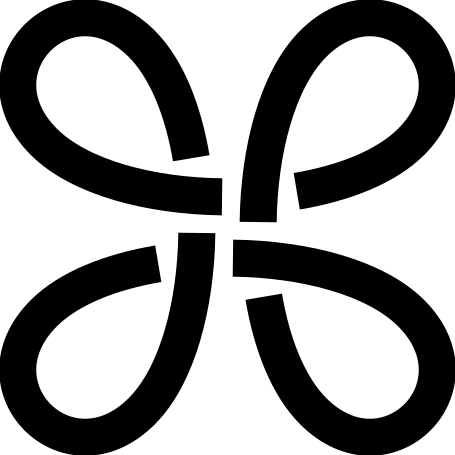
\includegraphics{logo.png}}

\begin{document}                      % начало документа

\maketitle

\tableofcontents

\newcounter{KnotNoName}\setcounter{KnotNoName}{0}
\newcounter{LoopNoName}\setcounter{LoopNoName}{0}
\newcounter{HitchNoName}\setcounter{HitchNoName}{0}
\newcounter{GachnyNoName}\setcounter{GachnyNoName}{0}
\newcounter{SamosbrosNoName}\setcounter{SamosbrosNoName}{0}
\newcounter{SheepshankNoName}\setcounter{SheepshankNoName}{0}

\chapter*{Введение}

\epigraph{\textit{There's a lot of virtue \\in a round turn}}{}

\lettrine[lines=3,loversize=0.2,nindent=4pt,slope=0pt]{З}{} адача этой книги состоит не в простом перечислении всех возможных или, наоборот, каких-то особенных узлов, как в большинстве подобных книг. Количество узлов (или их систем) бесконечно. Четкую грань между узлом и системой, состоящей из нескольких узлов, на мой взгляд, провести достаточно проблематично. Предлагаю рассматривать каждый узел как систему элементов, то есть более простых узлов.

Если раньше, в силу понятных причин, основными \enquote{изобретателями} узлов были моряки, то теперь это, конечно же альпинисты.

%TODO Добавить простые узлы.

Эти простые узлы, в свою очередь, состоят из еще более простых элементов.

Кроме того, любой узел можно усложнить. Существует несколько способов:

\begin{itemize}
	\item Шлаг на опоре с одного конца.
	\item Шлаг на опоре с обоих концов.
	\item Развернуть часть шлагов в другую сторону.
	\item Зафиксировать ходовой конец.
	\begin{itemize}
		\item На опоре.
		\item На коренном конце.
		\item В самом узле.
	\end{itemize}
	\item Использовать сразу несколько способов.
	\item Совместить вместе разные узлы.
\end{itemize}

Рисунки достаточно схематичны. Это сделано специально, именно для того, чтобы показать не внешний вид завязанного узла, а внутреннюю логику его построения.

Особое место в классификации узлов занимает их название. В разных источниках можно встретить как разные названия одного и того же узла, так и разные узлы под одним названием, даже у уважаемых авторов, таких как Л.Н. Скрягин\citep{Skryagin}, И.В. Балабанов\citep{Balabanov}, Clifford W. Ashley\citep{Ashley}, и Geoffrey Budworth\citep{Budworth} и других.

Чтобы было понятно, о чем речь, нужно последовать опыту древних китайских мудрецов. Перед философскими диспутами они сначала договаривались о терминах и определениях, чтобы говорить об одном и том же, а не каждый о своем.

Различия колышек и штыков. И то, и другое начинается с

\part{Виды узлов}

\chapter{Узлы одним концом}

\lettrine[lines=3,loversize=0.2,nindent=-3pt,slope=-3pt]{У}{} злы, завязанные одним концом троса, могут использоваться в разных целях. Например, для утолщения троса, предохранения его от расплетания прядей, формирования затягивающихся и незатягивающихся петель, а также для привязывания троса к чему-либо. Кроме того, существует масса декоративных вариантов, как плоских, так и объемных.

\section{Узлы для утолщения троса}

\section{Простые}

Обычно вяжутся на конце троса для предотвращения продергивания через блок или предотвращения расплетания прядей на концах многопрядных тросов.

\subsection{Простой узел}

\begin{figure}[H]\centering
	\subfloat[Левый]{\label{ris:Single_Knot_left}
	\tcbox[enhanced jigsaw,colframe=black,opacityframe=0.5,opacityback=0.5]
		{\centering
			\includesvg[width=0.33\linewidth]{Utolsh/Single_1}}
		}
\hfil
	\subfloat[Правый]{\label{ris:Single_Knot_right}
	\tcbox[enhanced jigsaw,colframe=black,opacityframe=0.5,opacityback=0.5]
		{\centering
			\includesvg[width=0.33\linewidth]{Utolsh/Single}}
		}
	\caption{Простой узел.}\label{ris:Single_Knot}
\end{figure}

Overhand, Simple, Single, Thumb, Common, Ordinary Knot. Русские названия - Калач, Обыкновенный узел.

Принцип Зеркалирования.

\subsection{Пожарная лестница}

\begin{figure}[H]\centering
	\subfloat[Завязывание]{\label{ris:Fire-Escape_1}
	\tcbox[enhanced jigsaw,colframe=black,opacityframe=0.5,opacityback=0.5]
		{\centering
			\includesvg[width=0.45\linewidth]{Utolsh/Fire-Escape}}
		}
\end{figure}
% \vfill
\begin{figure}[H]\centering
	\subfloat[Результат]{\label{ris:Fire-Escape_2}
	\tcbox[enhanced jigsaw,colframe=black,opacityframe=0.5,opacityback=0.5]
		{\centering
			\includesvg[width=0.7\linewidth]{Utolsh/Fire-Escape_1}}
		}
	\caption{Пожарная лестница.}\label{ris:Fire-Escape}
\end{figure}

Fire-Escape или Philadelphia Knot. Пожарная лестница, Шкентель с мусингами. Вязка этого узла начинается с формирования калышек, заведенных друг за друга. У вас получится некое подобие бухты. Ходовой конец пропустите внутрь нее. Медленно, без рывков, тяните за ходовой конец троса. По мере его вытягивания будут завязываться простые узлы. Их число будет соответствовать числу сделанных калышек, а расстояние между ними - длине их окружности.

\subsection{Бисерный узел}

\begin{figure}[H]\centering
	\begin{minipage}{1\linewidth}
		\begin{center}
			\tcbox[enhanced jigsaw,colframe=black,opacityframe=0.5,opacityback=0.5]
			{\includesvg[width=0.3\linewidth]{Utolsh/Bead_Knot}}
		\end{center}
	\end{minipage}
\caption{Бисерный узел}
	\label{ris:Bead_Knot}
\end{figure}

Bead Knot.

\subsection{True-Lover’s Knot}

\begin{figure}[H]\centering
	\begin{minipage}{1\linewidth}
		\begin{center}
			\tcbox[enhanced jigsaw,colframe=black,opacityframe=0.5,opacityback=0.5]
			{\includesvg[width=0.23\linewidth]{Utolsh/True-Lover_Knot}}
		\end{center}
	\end{minipage}
\caption{True-Lover’s Knot}
	\label{ris:True-Lover_Knot}
\end{figure}

Узел настоящих любовников.

\addtocounter{KnotNoName}{1}

\subsection{Узел без названия \arabic{KnotNoName}}

\begin{figure}[H]\centering
	\begin{minipage}{1\linewidth}
		\begin{center}
			\tcbox[enhanced jigsaw,colframe=black,opacityframe=0.5,opacityback=0.5]
			{\includesvg[width=0.25\linewidth]{Utolsh/KnotNoName_18}}
		\end{center}
	\end{minipage}
\caption{Узел без названия \arabic{KnotNoName}}
	\label{ris:KnotNoName_18}
\end{figure}

\addtocounter{KnotNoName}{1}

\subsection{Узел без названия \arabic{KnotNoName}}

\begin{figure}[H]\centering
	\begin{minipage}{1\linewidth}
		\begin{center}
			\tcbox[enhanced jigsaw,colframe=black,opacityframe=0.5,opacityback=0.5]
			{\includesvg[width=0.28\linewidth]{Utolsh/KnotNoName_3}}
		\end{center}
	\end{minipage}
\caption{Узел без названия \arabic{KnotNoName}}
	\label{ris:KnotNoName_3}
\end{figure}

\subsection{Королевский узел}

\begin{figure}[H]\centering
	\subfloat[Завязывание]{\label{ris:Tweenie_sposob}
	\tcbox[enhanced jigsaw,colframe=black,opacityframe=0.5,opacityback=0.5]
		{\centering
			\includesvg[width=0.33\linewidth]{Utolsh/Tweenie}}
		}
\hfil
	\subfloat[Результат]{\label{ris:Tweenie_rez}
	\tcbox[enhanced jigsaw,colframe=black,opacityframe=0.5,opacityback=0.5]
		{\centering
			\includesvg[width=0.33\linewidth]{Utolsh/Tweenie_1}}
		}
	\caption{Королевский узел.}\label{ris:Tweenie}
\end{figure}

Другое название - Tweenie.

\subsection{Апокрифический узел}

\begin{figure}[H]\centering
	\begin{minipage}{1\linewidth}
		\begin{center}
			\tcbox[enhanced jigsaw,colframe=black,opacityframe=0.5,opacityback=0.5]
			{\centering{\includesvg[width=0.35\linewidth]{Utolsh/Apokrif}}}
		\end{center}
	\end{minipage}
\caption{Апокрифический узел.}
	\label{ris:Apokrif}
\end{figure}

\subsection{Двойной Простой узел}

Double Overhand Knot, Blood Knot. Кровавый узел, Капуцин, Косичка стопорная, Двойной простой, среди альпинистов известен так же как БеК (бескарабинный).

\begin{figure}[H]\centering
	\subfloat[Первый вариант]{\label{ris:Double_Knot_1}
	\tcbox[enhanced jigsaw,colframe=black,opacityframe=0.5,opacityback=0.5]
		{\centering
			\includesvg[width=0.39\linewidth]{Utolsh/Double}}
		}
\hfil
	\subfloat[Первый способ вязки]{\label{ris:Double_Knot_sposob_1}
	\tcbox[enhanced jigsaw,colframe=black,opacityframe=0.5,opacityback=0.5]
		{\centering
			\includesvg[width=0.39\linewidth]{Utolsh/Double_1}}
		}
\end{figure}
% \vfill
\begin{figure}[H]\centering
	\subfloat[Второй вариант]{\label{ris:Double_Knot_2}
	\tcbox[enhanced jigsaw,colframe=black,opacityframe=0.5,opacityback=0.5,height=3cm]
		{\centering
			\includesvg[width=0.3\linewidth]{Utolsh/Double_3}}
		}
\hfil
	\subfloat[Второй способ вязки]{\label{ris:Double_Knot_sposob_2}
	\tcbox[enhanced jigsaw,colframe=black,opacityframe=0.5,opacityback=0.5,height=3cm]
		{\centering
			\includesvg[width=0.3\linewidth]{Utolsh/Double_2}}
		}
	\caption{Двойной Простой узел.}\label{ris:Double_Knot}
\end{figure}

При затягивании узел трансформируется. Особенно хорошо это видно при большом количество шлагов. Если потянуть в разные стороны ходовой и коренной концы, внешняя петля узла начинает свиваться, образуя несколько витков. Причем направление свивания будет противоположным направлению, в котором делались шлаги. Витков, охватывающих шлаги снаружи, получится тем больше, чем больше было сделано дополнительных шлагов. Перед окончательным затягиванием узла надо убедиться, что витки получились ровными, плотно прилегают, но не налезают друг на друга.

\subsection{Тройной Простой узел}

\begin{figure}[H]\centering
	\subfloat[Тройной]{\label{ris:Triple_Knot_1}
	\tcbox[enhanced jigsaw,colframe=black,opacityframe=0.5,opacityback=0.5,height=3cm]
		{\centering
			\includesvg[width=0.34\linewidth]{Utolsh/Triple_1}}
		}
\hfil
	\subfloat[Четверной]{\label{ris:Triple_Knot_2}
	\tcbox[enhanced jigsaw,colframe=black,opacityframe=0.5,opacityback=0.5,height=3cm]
		{\centering
			\includesvg[width=0.39\linewidth]{Utolsh/Triple_2}}
		}
\end{figure}

Threefold Overhand Knot, Triple Overhand Knot. Кровавый узел. Больше трех шлагов (четверной и далее) - Multiple Overhand Knot, другое название French Knot.

Можно завязать несколькими различными способами. Два из них представлены на рисунках \ref{ris:Double_Knot_sposob_1} и \ref{ris:Double_Knot_sposob_2}. Завязывая Простой узел (рис.~\ref{ris:Single_Knot}), делаем несколько дополнительных шлагов ходовым концом, чтобы получить тройной (и более) узел. Иногда отдельно выделяют третий способ вязки, но он является просто развитием первого способа.

\begin{figure}[H]\centering
	\subfloat[Завязывание]{\label{ris:Triple_Knot_sposob_1}
	\tcbox[enhanced jigsaw,colframe=black,opacityframe=0.5,opacityback=0.5,height=2.5cm]
		{\centering
			\includesvg[width=0.36\linewidth]{Utolsh/Triple_3}}
		}
\hfil
	\subfloat[Завязывание]{\label{ris:Triple_Knot_sposob_2}
	\tcbox[enhanced jigsaw,colframe=black,opacityframe=0.5,opacityback=0.5,height=2.5cm]
		{\centering
			\includesvg[width=0.36\linewidth]{Utolsh/Triple_4}}
		}
	\caption{Тройной Простой узел.}\label{ris:Triple_Knot}
\end{figure}

\subsection{Long Three-Ply Knot}

\begin{figure}[H]\centering
	\subfloat[Завязывание]{\label{ris:Long_Three-Ply_Knot_1}
	\tcbox[enhanced jigsaw,colframe=black,opacityframe=0.5,opacityback=0.5,height=3.5cm]
		{\centering
			\includesvg[width=0.33\linewidth]{Utolsh/Long_Three-Ply_Knot}}
		}
\hfil
	\subfloat[Завязывание]{\label{ris:Long_Three-Ply_Knot_2}
	\tcbox[enhanced jigsaw,colframe=black,opacityframe=0.5,opacityback=0.5,height=3.5cm]
		{\centering
			\includesvg[width=0.41\linewidth]{Utolsh/Long_Three-Ply_Knot_1}}
		}
\end{figure}
% \vfill
\begin{figure}[H]\centering
	\subfloat[Результат]{\label{ris:Long_Three-Ply_Knot_3}
	\tcbox[enhanced jigsaw,colframe=black,opacityframe=0.5,opacityback=0.5]
		{\centering
			\includesvg[width=0.5\linewidth]{Utolsh/Long_Three-Ply_Knot_2}}
		}
	\caption{Long Three-Ply Knot.}\label{ris:Long_Three-Ply_Knot}
\end{figure}

На рисунке \ref{ris:Long_Three-Ply_Knot_2} стрелками обозначены направления, в которых начнут скручиваться внешние петли при затягивании узла. Как и в Двойном Простом узле (рис.~\ref{ris:Double_Knot_2}), в процессе затягивания необходимо контролировать правильность и ровность прилегания витков.

\subsection{Восьмерка}

\begin{figure}[H]\centering
	\begin{minipage}{1\linewidth}
		\begin{center}
			\tcbox[enhanced jigsaw,colframe=black,opacityframe=0.5,opacityback=0.5]
			{\centering{\includesvg[width=0.3\linewidth]{Utolsh/Figure-Of-Eight}}}
		\end{center}
	\end{minipage}
\caption{Восьмерка}
	\label{ris:Figure-Of-Eight}
\end{figure}

Figure-Of-Eight Knot, Flemish Knot, Савойский узел.

\subsection{Юферсный узел}

\begin{figure}[H]\centering
	\subfloat[Первая схема]{\label{ris:Long_Three-Ply_Knot_1}
	\tcbox[enhanced jigsaw,colframe=black,opacityframe=0.5,opacityback=0.5,height=3.5cm]
		{\centering
			\includesvg[width=0.33\linewidth]{Utolsh/Ufers}}
		}
\hfil
	\subfloat[Вторая схема]{\label{ris:Long_Three-Ply_Knot_2}
	\tcbox[enhanced jigsaw,colframe=black,opacityframe=0.5,opacityback=0.5,height=3.5cm]
		{\centering
			\includesvg[width=0.33\linewidth]{Utolsh/Ufers_3}}
		}
\end{figure}
% \vfill
\begin{figure}[H]\centering
	\subfloat[Способ вязки из Простого узла (рис.~\ref{ris:Single_Knot})]{\label{ris:Ufers_sposob_1}
	\tcbox[enhanced jigsaw,colframe=black,opacityframe=0.5,opacityback=0.5,height=3.5cm]
		{\centering
			\includesvg[width=0.33\linewidth]{Utolsh/Ufers_1}}
		}
\hfil
	\subfloat[Способ вязки из Восьмерки (рис.~\ref{ris:Figure-Of-Eight})]{\label{ris:Ufers_sposob_2}
	\tcbox[enhanced jigsaw,colframe=black,opacityframe=0.5,opacityback=0.5,height=3.5cm]
		{\centering
			\includesvg[width=0.33\linewidth]{Utolsh/Ufers_2}}
		}
	\caption{Юферсный узел.}\label{ris:Ufers}
\end{figure}

Simple Lanyard Knot. Две схемы одного и того же узла.

\addtocounter{KnotNoName}{1}

\subsection{Узел без названия \arabic{KnotNoName}}

% FIXME Охотничий?

\begin{figure}[H]\centering
	\subfloat[Первая схема]{\label{ris:KnotNoName_5_1}
	\tcbox[enhanced jigsaw,colframe=black,opacityframe=0.5,opacityback=0.5,height=3.5cm]
		{\centering
			\includesvg[width=0.33\linewidth]{Utolsh/KnotNoName_5}}
		}
\hfil
	\subfloat[Вторая схема]{\label{ris:KnotNoName_5_2}
	\tcbox[enhanced jigsaw,colframe=black,opacityframe=0.5,opacityback=0.5,height=3.5cm]
		{\centering
			\includesvg[width=0.33\linewidth]{Utolsh/KnotNoName_5_1}}
		}
	\caption{Узел без названия \arabic{KnotNoName}.}\label{ris:KnotNoName_5}
\end{figure}

Так же как и на рис.~\ref{ris:Ufers} две схемы одного и того же узла.

\addtocounter{KnotNoName}{1}

\subsection{Узел без названия \arabic{KnotNoName}}

\begin{figure}[H]\centering
	\begin{minipage}{1\linewidth}
		\begin{center}
			\tcbox[enhanced jigsaw,colframe=black,opacityframe=0.5,opacityback=0.5]
			{\centering{\includesvg[width=0.4\linewidth]{Utolsh/KnotNoName_6}}}
		\end{center}
	\end{minipage}
\caption{Узел без названия \arabic{KnotNoName}.}
	\label{ris:KnotNoName_6}
\end{figure}

\addtocounter{KnotNoName}{1}

\subsection{Узел без названия \arabic{KnotNoName}}

%FIXME сделать узел для связывания двух тросов (рисунок внутри svg-файла)

\begin{figure}[H]\centering
	\begin{minipage}{1\linewidth}
		\begin{center}
			\tcbox[enhanced jigsaw,colframe=black,opacityframe=0.5,opacityback=0.5]
			{\centering{\includesvg[width=0.5\linewidth]{Utolsh/KnotNoName_7}}}
		\end{center}
	\end{minipage}
\caption{Узел без названия \arabic{KnotNoName}.}
	\label{ris:KnotNoName_7}
\end{figure}

\subsection{Филадельфийская лестница}

\begin{figure}[H]\centering
	\subfloat[Завязывание]{\label{ris:Continuous_Figure-of-Eight_1}
	\tcbox[enhanced jigsaw,colframe=black,opacityframe=0.5,opacityback=0.5,height=2.5cm]
		{\centering
			\includesvg[width=0.33\linewidth]{Utolsh/Continuous_Figure-of-Eight}}
		}
\end{figure}
% \vfill
\begin{figure}[H]\centering
	\subfloat[Результат]{\label{ris:Continuous_Figure-of-Eight_2}
	\tcbox[enhanced jigsaw,colframe=black,opacityframe=0.5,opacityback=0.5,height=2.5cm]
		{\centering
			\includesvg[width=0.5\linewidth]{Utolsh/Continuous_Figure-of-Eight_1}}
		}
	\caption{Филадельфийская лестница.}\label{ris:Continuous_Figure-of-Eight}
\end{figure}

Chain of Figure-Of-Eight Knots, Continuous Figure-of-Eight knot.

\subsection{Intermediate Knot}

% FIXME Девятка?

\begin{figure}[H]\centering
	\begin{minipage}{1\linewidth}
		\begin{center}
			\tcbox[enhanced jigsaw,colframe=black,opacityframe=0.5,opacityback=0.5]
			{\centering{\includesvg[width=0.5\linewidth]{Utolsh/Intermediate}}}
		\end{center}
	\end{minipage}
\caption{Intermediate Knot.}
	\label{ris:Intermediate}
\end{figure}

\subsection{Стивидорный узел}

\begin{figure}[H]\centering
	\begin{minipage}{1\linewidth}
		\begin{center}
			\tcbox[enhanced jigsaw,colframe=black,opacityframe=0.5,opacityback=0.5]
			{\centering{\includesvg[width=0.6\linewidth]{Utolsh/Stevedore}}}
		\end{center}
	\end{minipage}
\caption{Стивидорный узел.}
	\label{ris:Stevedore}
\end{figure}

Stevedore Knot.

\subsection{Многократная Восьмерка}

\begin{figure}[H]\centering
	\subfloat[Первый вариант]{\label{ris:Double_Figure-Of-Eight_1}
	\tcbox[enhanced jigsaw,colframe=black,opacityframe=0.5,opacityback=0.5,height=3.5cm]
		{\centering
			\includesvg[width=0.33\linewidth]{Utolsh/Double_Figure-Of-Eight}}
		}
\hfil
	\subfloat[Второй вариант]{\label{ris:Double_Figure-Of-Eight_2}
	\tcbox[enhanced jigsaw,colframe=black,opacityframe=0.5,opacityback=0.5,height=3.5cm]
		{\centering
			\includesvg[width=0.33\linewidth]{Utolsh/Double_Figure-Of-Eight_1}}
		}
\end{figure}
% \vfill
\begin{figure}[H]\centering
	\subfloat[Третий вариант]{\label{ris:Double_Figure-Of-Eight_3}
	\tcbox[enhanced jigsaw,colframe=black,opacityframe=0.5,opacityback=0.5,height=3.5cm]
		{\centering
			\includesvg[width=0.33\linewidth]{Utolsh/Double_Figure-Of-Eight_2}}
		}
\hfil
	\subfloat[Четвертый вариант]{\label{ris:Double_Figure-Of-Eight_4}
	\tcbox[enhanced jigsaw,colframe=black,opacityframe=0.5,opacityback=0.5,height=3.5cm]
		{\centering
			\includesvg[width=0.33\linewidth]{Utolsh/Double_Figure-Of-Eight_3}}
		}
	\caption{Многократная Восьмерка.}\label{ris:Double_Figure-Of-Eight}
\end{figure}

Double Figure-Of-Eight Knot. Многократная восьмерка, Косичка.

\subsection{Multiple Figure-Of-Eight Knot}

\begin{figure}[H]\centering
	\begin{minipage}{1\linewidth}
		\begin{center}
			\tcbox[enhanced jigsaw,colframe=black,opacityframe=0.5,opacityback=0.5]
			{\centering{\includesvg[width=0.7\linewidth]{Utolsh/Multiple_Figure-Of-Eight}}}
		\end{center}
	\end{minipage}
\caption{Multiple Figure-Of-Eight Knot.}
	\label{ris:Multiple_Figure-Of-Eight}
\end{figure}

Multiple Figure-Of-Eight Knot. Варианты вязки такие же как и у Многократной восьмерки (рис.~\ref{ris:Double_Figure-Of-Eight}).

\subsection{Стопорный узел Голдобина}

\begin{figure}[H]\centering
	\begin{minipage}{1\linewidth}
		\begin{center}
			\tcbox[enhanced jigsaw,colframe=black,opacityframe=0.5,opacityback=0.5]
			{\centering{\includesvg[width=0.35\linewidth]{Utolsh/Goldobin}}}
		\end{center}
	\end{minipage}
\caption{Стопорный узел Голдобина.}
	\label{ris:Goldobin}
\end{figure}

% TODO см. Anchor Bend Variant or Double Oysterman’s Knot???

Две петли и два шлага.\footnote{На этот узел в 1988 году Вениамином Федоровичем Голдобиным получено авторское свидетельство \href{http://patents.su/2-1434012-stopornyjj-uzel-goldobina.html}{№ SU 1434012}} Три петли и три шлага еще больше увеличат размер узла.

\subsection{Развязывающийся простой узел}

\begin{figure}[H]\centering
	\begin{minipage}{1\linewidth}
		\begin{center}
			\tcbox[enhanced jigsaw,colframe=black,opacityframe=0.5,opacityback=0.5]
			{\centering{\includesvg[width=0.5\linewidth]{Utolsh/Slip_Knot}}}
		\end{center}
	\end{minipage}
\caption{Развязывающийся простой узел.}
	\label{ris:Slip_Knot}
\end{figure}

Slip Knot. Фактически, это Арбор или Simple Noose (рис.~\ref{ris:Arbor}). Отличие только в назначении узлов. Арбор - затягивающаяся петля, которая скользит по коренному концу, а Развязывающийся простой узел служит для утолщения троса с возможностью быстрого развязывания. В связи с этим коренной конец у него тот, который в Арборе является ходовым. Кроме того, это еще и Slipped Half Hitch (рис.~\ref{ris:Slipped_Half_Hitch}), который используется для привязывания к опоре. В принципе, таким образом можно использовать любую быстроразвязывающуюся петлю (см. рис.~\ref{ris:Slip_Figure-Of-Eight})

\subsection{Устричный узел}

\begin{figure}[H]\centering
	\subfloat[Завязывание]{\label{ris:Oysterman_1}
	\tcbox[enhanced jigsaw,colframe=black,opacityframe=0.5,opacityback=0.5,height=3.5cm]
		{\centering
			\includesvg[width=0.39\linewidth]{Utolsh/Oysterman}}
		}
\hfil
	\subfloat[Результат]{\label{ris:Oysterman_2}
	\tcbox[enhanced jigsaw,colframe=black,opacityframe=0.5,opacityback=0.5,height=3.5cm]
		{\centering
			\includesvg[width=0.27\linewidth]{Utolsh/Oysterman_1}}
		}
	\caption{Устричный узел.}\label{ris:Oysterman}
\end{figure}

Oysterman’s Stopper Knot, Ashley’s Stopper Knot. Вяжется из Развязывающегося простого узла (рис.~\ref{ris:Arbor}).

\addtocounter{KnotNoName}{1}

\subsection{Узел без названия \arabic{KnotNoName}}

\begin{figure}[H]\centering
	\subfloat[Завязывание]{\label{ris:KnotNoName_4_1}
	\tcbox[enhanced jigsaw,colframe=black,opacityframe=0.5,opacityback=0.5,height=3.5cm]
		{\centering
			\includesvg[width=0.38\linewidth]{Utolsh/KnotNoName_4}}
		}
\hfil
	\subfloat[Результат]{\label{ris:KnotNoName_4_2}
	\tcbox[enhanced jigsaw,colframe=black,opacityframe=0.5,opacityback=0.5,height=3.5cm]
		{\centering
			\includesvg[width=0.38\linewidth]{Utolsh/KnotNoName_4_1}}
		}
	\caption{Узел без названия \arabic{KnotNoName}.}\label{ris:KnotNoName_4}
\end{figure}

Как и Устричный узел (рис.~\ref{ris:Oysterman}), этот узел на основе Развязывающегося простого узла (рис.~\ref{ris:Arbor}).

\subsection{Развязывающаяся восьмерка}

\begin{figure}[H]\centering
	\begin{minipage}{1\linewidth}
		\begin{center}
			\tcbox[enhanced jigsaw,colframe=black,opacityframe=0.5,opacityback=0.5]
			{\centering{\includesvg[width=0.4\linewidth]{Utolsh/Slip_Figure-Of-Eight}}}
		\end{center}
	\end{minipage}
\caption{Развязывающаяся восьмерка.}
	\label{ris:Slip_Figure-Of-Eight}
\end{figure}

Slip Figure-Of-Eight Knot. Используется так же как Развязывающийся простой узел (рис.~\ref{ris:Slip_Knot})

\subsection{Стратим}

\begin{figure}[H]\centering
	\subfloat[Первый вариант]{\label{ris:Stratim_1}
	\tcbox[enhanced jigsaw,colframe=black,opacityframe=0.5,opacityback=0.5]
		{\centering
			\includesvg[width=0.38\linewidth]{Utolsh/Stratim}}
		}
\hfil
	\subfloat[Второй вариант]{\label{ris:Stratim_2}
	\tcbox[enhanced jigsaw,colframe=black,opacityframe=0.5,opacityback=0.5]
		{\centering
			\includesvg[width=0.38\linewidth]{Utolsh/Stratim_1}}
		}
	\caption{Стратим.}\label{ris:Stratim}
\end{figure}


\section{Легости}

В гражданском и речном флотах так называется бросательный конец.

\subsection{Францисканский узел}

\begin{figure}[H]\centering
	\begin{minipage}{1\linewidth}
		\begin{center}
			\tcbox[enhanced jigsaw,colframe=black,opacityframe=0.5,opacityback=0.5]
			{\centering{\includesvg[width=0.5\linewidth]{Utolsh/Francisk}}}
		\end{center}
	\end{minipage}
\caption{Францисканский узел.}
	\label{ris:Francisk}
\end{figure}

Он же Капуцин.

\subsection{Norfolk-to-Washington}

\begin{figure}[H]\centering
	\begin{minipage}{1\linewidth}
		\begin{center}
			\tcbox[enhanced jigsaw,colframe=black,opacityframe=0.5,opacityback=0.5]
			{\centering{\includesvg[width=0.65\linewidth]{Utolsh/Norfolk-to-Washington}}}
		\end{center}
	\end{minipage}
\caption{Norfolk-to-Washington.}
	\label{ris:Norfolk-to-Washington}
\end{figure}

\subsection{Boat Heaving Line Knot}

\begin{figure}[H]\centering
	\begin{minipage}{1\linewidth}
		\begin{center}
			\tcbox[enhanced jigsaw,colframe=black,opacityframe=0.5,opacityback=0.5]
			{\centering{\includesvg[width=0.8\linewidth]{Utolsh/Heaving_Line_Knot}}}
		\end{center}
	\end{minipage}
\caption{Boat Heaving Line Knot.}
	\label{ris:Heaving_Line_Knot}
\end{figure}

\subsection{Hangman’s Knot}

\begin{figure}[H]\centering
	\begin{minipage}{1\linewidth}
		\begin{center}
			\tcbox[enhanced jigsaw,colframe=black,opacityframe=0.5,opacityback=0.5]
			{\centering{\includesvg[width=0.8\linewidth]{Utolsh/Hangman_Knot}}}
		\end{center}
	\end{minipage}
\caption{Hangman’s Knot.}
	\label{ris:Hangman_Knot}
\end{figure}

\subsection{Over-and-Under Heaving Line Knot}

\begin{figure}[H]\centering
	\begin{minipage}{1\linewidth}
		\begin{center}
			\tcbox[enhanced jigsaw,colframe=black,opacityframe=0.5,opacityback=0.5]
			{\centering{\includesvg[width=0.8\linewidth]{Utolsh/Over-and-Under}}}
		\end{center}
	\end{minipage}
\caption{Over-and-Under Heaving Line Knot.}
	\label{ris:Over-and-Under}
\end{figure}

\subsection{Двойной Францисканский узел}

\begin{figure}[H]\centering
	\begin{minipage}{1\linewidth}
		\begin{center}
			\tcbox[enhanced jigsaw,colframe=black,opacityframe=0.5,opacityback=0.5]
			{\centering{\includesvg[width=0.5\linewidth]{Utolsh/Double_Francisk}}}
		\end{center}
	\end{minipage}
\caption{Двойной Францисканский узел.}
	\label{ris:Double_Francisk}
\end{figure}

Двойной Капуцин.



\section{Декоративные}

\addtocounter{KnotNoName}{1}

\subsection{Узел без названия \arabic{KnotNoName}}

\begin{figure}[H]\centering
	\subfloat[Завязывание]{\label{ris:KnotNoName_9_1}
	\tcbox[enhanced jigsaw,colframe=black,opacityframe=0.5,opacityback=0.5,height=5cm]
		{\centering
			\includesvg[width=0.31\linewidth]{Utolsh/KnotNoName_9_1}}
		}
\hfil
	\subfloat[Результат]{\label{ris:KnotNoName_9_2}
	\tcbox[enhanced jigsaw,colframe=black,opacityframe=0.5,opacityback=0.5,height=5cm]
		{\centering
			\includesvg[width=0.35\linewidth]{Utolsh/KnotNoName_9}}
		}
	\caption{Узел без названия \arabic{KnotNoName}.}\label{ris:KnotNoName_9}
\end{figure}

\subsection{Трехпетельный узел}

\begin{figure}[H]\centering
	\subfloat[Завязывание]{\label{ris:TriplLoop_1}
	\tcbox[enhanced jigsaw,colframe=black,opacityframe=0.5,opacityback=0.5,height=4cm]
		{\centering
			\includesvg[width=0.38\linewidth]{Utolsh/TriplLoop}}
		}
\hfil
	\subfloat[Завязывание]{\label{ris:TriplLoop_2}
	\tcbox[enhanced jigsaw,colframe=black,opacityframe=0.5,opacityback=0.5,height=4cm]
		{\centering
			\includesvg[width=0.26\linewidth]{Utolsh/TriplLoop_2}}
		}
\end{figure}
% \vfill
\begin{figure}[H]\centering
	\subfloat[Результат]{\label{ris:TriplLoop_3}
	\tcbox[enhanced jigsaw,colframe=black,opacityframe=0.5,opacityback=0.5]
		{\centering
			\includesvg[width=0.33\linewidth]{Utolsh/TriplLoop_1}}
		}
	\caption{Трехпетельный узел.}\label{ris:TriplLoop}
\end{figure}

Three-Ply Knot. Результат похож на Устричный узел (рис.~\ref{ris:Oysterman}).

\subsection{Кордовый узел}

\begin{figure}[H]\centering
	\begin{minipage}{1\linewidth}
		\begin{center}
			\tcbox[enhanced jigsaw,colframe=black,opacityframe=0.5,opacityback=0.5]
			{\centering{\includesvg[width=0.35\linewidth]{Utolsh/Kord}}}
		\end{center}
	\end{minipage}
\caption{Кордовый узел.}
	\label{ris:Kord}
\end{figure}

One-Cord Knot.

\subsection{Японский венценосный узел}

\begin{figure}[H]\centering
	\begin{minipage}{1\linewidth}
		\begin{center}
			\tcbox[enhanced jigsaw,colframe=black,opacityframe=0.5,opacityback=0.5]
			{\centering{\includesvg[width=0.35\linewidth]{Utolsh/Japan}}}
		\end{center}
	\end{minipage}
\caption{Японский венценосный узел.}
	\label{ris:Japan}
\end{figure}

Другое название - Узел успеха.

\subsection{Узел Анны Богемской}

\begin{figure}[H]\centering
	\begin{minipage}{1\linewidth}
		\begin{center}
			\tcbox[enhanced jigsaw,colframe=black,opacityframe=0.5,opacityback=0.5]
			{\centering{\includesvg[width=0.35\linewidth]{Utolsh/Bogemia}}}
		\end{center}
	\end{minipage}
\caption{Узел Анны Богемской.}
	\label{ris:Bogemia}
\end{figure}

\subsection{Стопорный узел Шамова}

% TODO Наверняка он есть еще где-нибудь (в декоративных)!

\begin{figure}[H]\centering
	\subfloat[Завязывание]{\label{ris:Shamov_1}
	\tcbox[enhanced jigsaw,colframe=black,opacityframe=0.5,opacityback=0.5,height=4.5cm]
		{\centering
			\includesvg[width=0.33\linewidth]{Utolsh/Shamov}}
		}
\hfil
	\subfloat[Результат]{\label{ris:Shamov_2}
	\tcbox[enhanced jigsaw,colframe=black,opacityframe=0.5,opacityback=0.5,height=4.5cm]
		{\centering
			\includesvg[width=0.33\linewidth]{Utolsh/Shamov_1}}
		}
	\caption{Стопорный узел Шамова.}\label{ris:Shamov}
\end{figure}

Узел описан в книге А.П. Шамова \enquote{Способы и схемы вязки узлов и их применение в туристической практике}\citep{Shamov}.

\addtocounter{KnotNoName}{1}

\subsection{Узел без названия \arabic{KnotNoName}}

\begin{figure}[H]\centering
	\begin{minipage}{1\linewidth}
		\begin{center}
			\tcbox[enhanced jigsaw,colframe=black,opacityframe=0.5,opacityback=0.5]
			{\centering{\includesvg[width=0.35\linewidth]{Utolsh/KnotNoName_10}}}
		\end{center}
	\end{minipage}
\caption{Узел без названия \arabic{KnotNoName}.}
	\label{ris:KnotNoName_10}
\end{figure}

При затягивании получится петля из Плоского узла, похожая на Carrick Loop (рис.~\ref{ris:Carrick_Loop}).

\subsection{Четырехпетельный узел}

\begin{figure}[H]\centering
	\subfloat[Завязывание]{\label{ris:FourLoop_1_1}
	\tcbox[enhanced jigsaw,colframe=black,opacityframe=0.5,opacityback=0.5,height=4.5cm]
		{\centering
			\includesvg[width=0.34\linewidth]{Utolsh/FourLoop_2}}
		}
\hfil
	\subfloat[Результат]{\label{ris:FourLoop_1_2}
	\tcbox[enhanced jigsaw,colframe=black,opacityframe=0.5,opacityback=0.5,height=4.5cm]
		{\centering
			\includesvg[width=0.32\linewidth]{Utolsh/FourLoop_3}}
		}
	\caption{Четырехпетельный узел.}\label{ris:FourLoop}
\end{figure}

Four-Ply Knot.

\subsection{Четырехпетельный узел 2}

\begin{figure}[H]\centering
	\subfloat[Завязывание]{\label{ris:FourLoop_2_1}
	\tcbox[enhanced jigsaw,colframe=black,opacityframe=0.5,opacityback=0.5,height=4.5cm]
		{\centering
			\includesvg[width=0.4\linewidth]{Utolsh/FourLoop}}
		}
\hfil
	\subfloat[Результат]{\label{ris:FourLoop_2_2}
	\tcbox[enhanced jigsaw,colframe=black,opacityframe=0.5,opacityback=0.5,height=4.5cm]
		{\centering
			\includesvg[width=0.32\linewidth]{Utolsh/FourLoop_1}}
		}
	\caption{Четырехпетельный узел 2.}\label{ris:FourLoop_2}
\end{figure}

Double Three-Ply Knot.

\subsection{Наполеон}

\begin{figure}[H]\centering
	\begin{minipage}{1\linewidth}
		\begin{center}
			\tcbox[enhanced jigsaw,colframe=black,opacityframe=0.5,opacityback=0.5]
			{\centering{\includesvg[width=0.35\linewidth]{Utolsh/Napoleon}}}
		\end{center}
	\end{minipage}
\caption{Наполеон.}
\label{ris:Napoleon}
\end{figure}

\subsection{Китайский ткацкий узел}

\begin{figure}[H]\centering
	\begin{minipage}{1\linewidth}
		\begin{center}
			\tcbox[enhanced jigsaw,colframe=black,opacityframe=0.5,opacityback=0.5]
			{\centering{\includesvg[width=0.4\linewidth]{Utolsh/Chinese_tkach}}}
		\end{center}
	\end{minipage}
\caption{Китайский ткацкий узел.}
\label{ris:Chinese_tkach}
\end{figure}

% TODO нарисовать способ вязки

Five-Strand French Sinnet.

\addtocounter{KnotNoName}{1}

\subsection{Узел без названия \arabic{KnotNoName}}

\begin{figure}[H]\centering
	\begin{minipage}{1\linewidth}
		\begin{center}
			\tcbox[enhanced jigsaw,colframe=black,opacityframe=0.5,opacityback=0.5]
			{\centering{\includesvg[width=0.35\linewidth]{Utolsh/KnotNoName_1}}}
		\end{center}
	\end{minipage}
\caption{Узел без названия \arabic{KnotNoName}.}
\label{ris:KnotNoName_1}
\end{figure}

\addtocounter{KnotNoName}{1}

\subsection{Узел без названия \arabic{KnotNoName}}

\begin{figure}[H]\centering
	\begin{minipage}{1\linewidth}
		\begin{center}
			\tcbox[enhanced jigsaw,colframe=black,opacityframe=0.5,opacityback=0.5]
			{\centering{\includesvg[width=0.35\linewidth]{Utolsh/KnotNoName_8}}}
		\end{center}
	\end{minipage}
\caption{Узел без названия \arabic{KnotNoName}.}
\label{ris:KnotNoName_8}
\end{figure}

\addtocounter{KnotNoName}{1}

\subsection{Узел без названия \arabic{KnotNoName}}

\begin{figure}[H]\centering
	\begin{minipage}{1\linewidth}
		\begin{center}
			\tcbox[enhanced jigsaw,colframe=black,opacityframe=0.5,opacityback=0.5]
			{\centering{\includesvg[width=0.3\linewidth]{Utolsh/KnotNoName_2}}}
		\end{center}
	\end{minipage}
\caption{Узел без названия \arabic{KnotNoName}.}
\label{ris:KnotNoName_2}
\end{figure}

\addtocounter{KnotNoName}{1}

\subsection{Узел без названия \arabic{KnotNoName}}

\begin{figure}[H]\centering
	\begin{minipage}{1\linewidth}
		\begin{center}
			\tcbox[enhanced jigsaw,colframe=black,opacityframe=0.5,opacityback=0.5]
			{\centering{\includesvg[width=0.5\linewidth]{Utolsh/KnotNoName_16}}}
		\end{center}
	\end{minipage}
\caption{Узел без названия \arabic{KnotNoName}.}
\label{ris:KnotNoName_16}
\end{figure}

\subsection{Terminal Knot}

\begin{figure}[H]\centering
	\begin{minipage}{1\linewidth}
		\begin{center}
			\tcbox[enhanced jigsaw,colframe=black,opacityframe=0.5,opacityback=0.5]
			{\centering{\includesvg[width=0.35\linewidth]{Utolsh/Decorative_Terminal}}}
		\end{center}
	\end{minipage}
\caption{Terminal Knot.}
\label{ris:Decorative_Terminal}
\end{figure}

\subsection{Decorative Terminal Knot}

\begin{figure}[H]\centering
	\begin{minipage}{1\linewidth}
		\begin{center}
			\tcbox[enhanced jigsaw,colframe=black,opacityframe=0.5,opacityback=0.5]
			{\centering{\includesvg[width=0.35\linewidth]{Utolsh/Decorative_Terminal_1}}}
		\end{center}
	\end{minipage}
\caption{Terminal Knot.}
\label{ris:Decorative_Terminal_1}
\end{figure}

\subsection{Quatrefoil}

\begin{figure}[H]\centering
	\subfloat[Завязывание]{\label{ris:Quatrefoil_1}
	\tcbox[enhanced jigsaw,colframe=black,opacityframe=0.5,opacityback=0.5,height=5.5cm]
		{\centering
			\includesvg[width=0.3\linewidth]{Utolsh/Quatrefoil}}
		}
\hfil
	\subfloat[Результат]{\label{ris:Quatrefoil_2}
	\tcbox[enhanced jigsaw,colframe=black,opacityframe=0.5,opacityback=0.5,height=5.5cm]
		{\centering
			\includesvg[width=0.3\linewidth]{Utolsh/Quatrefoil_1}}
		}
	\caption{Quatrefoil.}\label{ris:Quatrefoil}
\end{figure}

\subsection{Cinquefoil}

\begin{figure}[H]\centering
	\begin{minipage}{1\linewidth}
		\begin{center}
			\tcbox[enhanced jigsaw,colframe=black,opacityframe=0.5,opacityback=0.5]
			{\centering{\includesvg[width=0.5\linewidth]{Utolsh/Cinquefoil}}}
		\end{center}
	\end{minipage}
\caption{Cinquefoil.}
\label{ris:Cinquefoil}
\end{figure}

\subsection{Двойной Устричный узел}

\begin{figure}[H]\centering
	\begin{minipage}{1\linewidth}
		\begin{center}
			\tcbox[enhanced jigsaw,colframe=black,opacityframe=0.5,opacityback=0.5]
			{\centering{\includesvg[width=0.5\linewidth]{Utolsh/Double_Oysterman}}}
		\end{center}
	\end{minipage}
\caption{Двойной Устричный узел.}
\label{ris:Double_Oysterman}
\end{figure}

Double Oysterman’s Knot.

\subsection{Настоящий Двойной Устричный узел}

\begin{figure}[H]\centering
	\begin{minipage}{1\linewidth}
		\begin{center}
			\tcbox[enhanced jigsaw,colframe=black,opacityframe=0.5,opacityback=0.5]
			{\centering{\includesvg[width=0.5\linewidth]{Utolsh/Truly_Double_Oysterman}}}
		\end{center}
	\end{minipage}
\caption{Настоящий Двойной Устричный узел.}
\label{ris:Truly_Double_Oysterman}
\end{figure}

Truly Double Oysterman’s Knot.

\subsection{Двойной Трехпетельный узел}

\begin{figure}[H]\centering
	\begin{minipage}{1\linewidth}
		\begin{center}
			\tcbox[enhanced jigsaw,colframe=black,opacityframe=0.5,opacityback=0.5]
			{\centering{\includesvg[width=0.4\linewidth]{Utolsh/Double_Three-Ply_Knot}}}
		\end{center}
	\end{minipage}
\caption{Двойной Трехпетельный узел.}
\label{ris:Double_Three-Ply_Knot}
\end{figure}

Double Three-Ply Knot.


\section{Голова турка} \label{chapter_Turk-Head}

\subsection{Two-Bight One-Lead Turk’s-Head}

\begin{figure}[H]\centering
	\begin{minipage}{1\linewidth}
		\begin{center}
			\tcbox[enhanced jigsaw,colframe=black,opacityframe=0.5,opacityback=0.5]
			{\centering{\includesvg[width=0.3\linewidth]{Utolsh/Turk-Head_1}}}
		\end{center}
	\end{minipage}
\caption{Two-Bight One-Lead Turk’s-Head.}
\label{ris:Turk-Head_1}
\end{figure}

Самая маленькая Голова Турка.

\subsection{Two-Bight Two-Lead Turk’s-Head}

\begin{figure}[H]\centering
	\begin{minipage}{1\linewidth}
		\begin{center}
			\tcbox[enhanced jigsaw,colframe=black,opacityframe=0.5,opacityback=0.5]
			{\centering{\includesvg[width=0.3\linewidth]{Utolsh/Turk-Head_2}}}
		\end{center}
	\end{minipage}
\caption{Two-Bight Two-Lead Turk’s-Head.}
\label{ris:Turk-Head_2}
\end{figure}

\subsection{Two-Bight Three-Lead Turk’s-Head}

\begin{figure}[H]\centering
	\begin{minipage}{1\linewidth}
		\begin{center}
			\tcbox[enhanced jigsaw,colframe=black,opacityframe=0.5,opacityback=0.5]
			{\centering{\includesvg[width=0.4\linewidth]{Utolsh/Turk-Head_3}}}
		\end{center}
	\end{minipage}
\caption{Two-Bight Three-Lead Turk’s-Head.}
\label{ris:Turk-Head_3}
\end{figure}

\subsection{Three-Bight Four-Lead triangular Turk’s-Head}

\begin{figure}[H]\centering
	\begin{minipage}{1\linewidth}
		\begin{center}
			\tcbox[enhanced jigsaw,colframe=black,opacityframe=0.5,opacityback=0.5]
			{\centering{\includesvg[width=0.45\linewidth]{Utolsh/Turk-Head_4}}}
		\end{center}
	\end{minipage}
\caption{Three-Bight Four-Lead triangular Turk’s-Head.}
\label{ris:Turk-Head_4}
\end{figure}

\subsection{Three-Bight Five-Lead Turk’s-Head}

\begin{figure}[H]\centering
	\begin{minipage}{1\linewidth}
		\begin{center}
			\tcbox[enhanced jigsaw,colframe=black,opacityframe=0.5,opacityback=0.5]
			{\centering{\includesvg[width=0.6\linewidth]{Utolsh/Turk-Head_5}}}
		\end{center}
	\end{minipage}
\caption{Three-Bight Five-Lead Turk’s-Head.}
\label{ris:Turk-Head_5}
\end{figure}

\subsection{Four-Bight Five-Lead Turk’s-Head}

% TODO Проверить схему

\begin{figure}[H]\centering
	\begin{minipage}{1\linewidth}
		\begin{center}
			\tcbox[enhanced jigsaw,colframe=black,opacityframe=0.5,opacityback=0.5]
			{\centering{\includesvg[width=0.45\linewidth]{Utolsh/Turk-Head_6}}}
		\end{center}
	\end{minipage}
\caption{Four-Bight Five-Lead Turk’s-Head.}
\label{ris:Turk-Head_6}
\end{figure}

\subsection{Four-Bight Six-Lead Turk’s-Head}

\begin{figure}[H]\centering
	\begin{minipage}{1\linewidth}
		\begin{center}
			\tcbox[enhanced jigsaw,colframe=black,opacityframe=0.5,opacityback=0.5]
			{\centering{\includesvg[width=0.5\linewidth]{Utolsh/Turk-Head_7}}}
		\end{center}
	\end{minipage}
\caption{Four-Bight Six-Lead Turk’s-Head.}
\label{ris:Turk-Head_7}
\end{figure}

\subsection{Eight-Lead Three-Bight Turk’s-Head}

\begin{figure}[H]\centering
	\begin{minipage}{1\linewidth}
		\begin{center}
			\tcbox[enhanced jigsaw,colframe=black,opacityframe=0.5,opacityback=0.5]
			{\centering{\includesvg[width=0.6\linewidth]{Utolsh/Turk-Head_8}}}
		\end{center}
	\end{minipage}
\caption{Eight-Lead Three-Bight Turk’s-Head.}
\label{ris:Turk-Head_8}
\end{figure}

Toggle-Shaped Knot.



\section{Косички и маты}

\subsection{На основе Простого узла}

\begin{figure}[H]\centering
	\subfloat[Завязывание]{\label{ris:Single_braid_1}
	\tcbox[enhanced jigsaw,colframe=black,opacityframe=0.5,opacityback=0.5,height=2.5cm]
		{\centering
			\includesvg[width=0.33\linewidth]{Utolsh/Single_braid}}
		}
\hfil
	\subfloat[Завязывание]{\label{ris:Single_braid_2}
	\tcbox[enhanced jigsaw,colframe=black,opacityframe=0.5,opacityback=0.5,height=2.5cm]
		{\centering
			\includesvg[width=0.33\linewidth]{Utolsh/Single_braid_1}}
		}
\end{figure}
% \vfill
\begin{figure}[H]\centering
	\subfloat[Результат]{\label{ris:Single_braid_3}
	\tcbox[enhanced jigsaw,colframe=black,opacityframe=0.5,opacityback=0.5]
		{\centering
			\includesvg[width=0.33\linewidth]{Utolsh/Single_braid_2}}
		}
	\caption{Косичка на основе Простого узла (рис.~\ref{ris:Single_Knot}).}\label{ris:Single_braid}
\end{figure}

\subsection{На основе Восьмерки}

\begin{figure}[H]\centering
	\subfloat[Завязывание]{\label{ris:Figure-Of-Eight_braid_1}
	\tcbox[enhanced jigsaw,colframe=black,opacityframe=0.5,opacityback=0.5,height=2.5cm]
		{\centering
			\includesvg[width=0.33\linewidth]{Utolsh/Figure-Of-Eight_braid}}
		}
\hfil
	\subfloat[Результат]{\label{ris:Figure-Of-Eight_braid_2}
	\tcbox[enhanced jigsaw,colframe=black,opacityframe=0.5,opacityback=0.5,height=2.5cm]
		{\centering
			\includesvg[width=0.33\linewidth]{Utolsh/Figure-Of-Eight_braid_1}}
		}
	\caption{Косичка на основе Восьмерки (рис.~\ref{ris:Figure-Of-Eight}).}\label{ris:Figure-Of-Eight_braid}
\end{figure}

\subsection{Двойная косичка из Простого узла}

\begin{figure}[H]\centering
	\subfloat[Завязывание]{\label{ris:Double_Single_braid_1}
	\tcbox[enhanced jigsaw,colframe=black,opacityframe=0.5,opacityback=0.5]
		{\centering
			\includesvg[width=0.35\linewidth]{Utolsh/Double_Single_braid}}
		}
\end{figure}
% \vfill
\begin{figure}[H]\centering
	\subfloat[Результат]{\label{ris:Double_Single_braid_2}
	\tcbox[enhanced jigsaw,colframe=black,opacityframe=0.5,opacityback=0.5]
		{\centering
			\includesvg[width=0.6\linewidth]{Utolsh/Double_Single_braid_1}}
		}
	\caption{Двойная косичка из Простого узла.}\label{ris:Double_Single_braid}
\end{figure}

Double Twist Braid Knot based on an Overhand Knot.

\subsection{Двойная косичка из Восьмерки}

\begin{figure}[H]\centering
	\subfloat[Завязывание]{\label{ris:Double_Figure-Of-Eight_braid_1}
	\tcbox[enhanced jigsaw,colframe=black,opacityframe=0.5,opacityback=0.5]
		{\centering
			\includesvg[width=0.45\linewidth]{Utolsh/Double_Figure-Of-Eight_braid}}
		}
\end{figure}
% \vfill
\begin{figure}[H]\centering
	\subfloat[Результат]{\label{ris:Double_Figure-Of-Eight_braid_2}
	\tcbox[enhanced jigsaw,colframe=black,opacityframe=0.5,opacityback=0.5]
		{\centering
			\includesvg[width=0.65\linewidth]{Utolsh/Double_Figure-Of-Eight_braid_1}}
		}
	\caption{Двойная косичка из Восьмерки.}\label{ris:Double_Figure-Of-Eight_braid}
\end{figure}

\subsection{Five-Lead Flat-Sinnet Terminal Knot}

\begin{figure}[H]\centering
	\subfloat[Завязывание]{\label{ris:Five-Lead_Flat-Sinnet_Terminal_Knot_1_1}
	\tcbox[enhanced jigsaw,colframe=black,opacityframe=0.5,opacityback=0.5,height=2.5cm]
		{\centering
			\includesvg[width=0.3\linewidth]{Utolsh/Five-Lead_Flat-Sinnet_Terminal_Knot}}
		}
\hfil
	\subfloat[Завязывание]{\label{ris:Five-Lead_Flat-Sinnet_Terminal_Knot_1_2}
	\tcbox[enhanced jigsaw,colframe=black,opacityframe=0.5,opacityback=0.5,height=2.5cm]
		{\centering
			\includesvg[width=0.45\linewidth]{Utolsh/Five-Lead_Flat-Sinnet_Terminal_Knot_1}}
		}
\end{figure}
% \vfill
\begin{figure}[H]\centering
	\subfloat[Завязывание]{\label{ris:Five-Lead_Flat-Sinnet_Terminal_Knot_1_3}
	\tcbox[enhanced jigsaw,colframe=black,opacityframe=0.5,opacityback=0.5]
		{\centering
			\includesvg[width=0.5\linewidth]{Utolsh/Five-Lead_Flat-Sinnet_Terminal_Knot_1_1}}
		}
\end{figure}
% \vfill
\begin{figure}[H]\centering
	\subfloat[Завязывание]{\label{ris:Five-Lead_Flat-Sinnet_Terminal_Knot_1_4}
	\tcbox[enhanced jigsaw,colframe=black,opacityframe=0.5,opacityback=0.5]
		{\centering
			\includesvg[width=0.55\linewidth]{Utolsh/Five-Lead_Flat-Sinnet_Terminal_Knot_1_2}}
		}
\end{figure}
% \vfill
\begin{figure}[H]\centering
	\subfloat[Завязывание]{\label{ris:Five-Lead_Flat-Sinnet_Terminal_Knot_1_5}
	\tcbox[enhanced jigsaw,colframe=black,opacityframe=0.5,opacityback=0.5]
		{\centering
			\includesvg[width=0.6\linewidth]{Utolsh/Five-Lead_Flat-Sinnet_Terminal_Knot_1_3}}
		}
\end{figure}
% \vfill
\begin{figure}[H]\centering
	\subfloat[Результат]{\label{ris:Five-Lead_Flat-Sinnet_Terminal_Knot_1_6}
	\tcbox[enhanced jigsaw,colframe=black,opacityframe=0.5,opacityback=0.5]
		{\centering
			\includesvg[width=0.65\linewidth]{Utolsh/Five-Lead_Flat-Sinnet_Terminal_Knot_1_4}}
		}
	\caption{Five-Lead Flat-Sinnet Terminal Knot.}\label{ris:Five-Lead_Flat-Sinnet_Terminal_Knot_1}
\end{figure}

\subsection{Five-Lead Flat-Sinnet Terminal Knot 2}

\begin{figure}[H]\centering
	\subfloat[Завязывание]{\label{ris:Five-Lead_Flat-Sinnet_Terminal_Knot_2_1}
	\tcbox[enhanced jigsaw,colframe=black,opacityframe=0.5,opacityback=0.5]
		{\centering
			\includesvg[width=0.3\linewidth]{Utolsh/Five-Lead_Flat-Sinnet_Terminal_Knot_2}}
		}
\end{figure}
% \vfill
\begin{figure}[H]\centering
	\subfloat[Завязывание]{\label{ris:Five-Lead_Flat-Sinnet_Terminal_Knot_2_2}
	\tcbox[enhanced jigsaw,colframe=black,opacityframe=0.5,opacityback=0.5]
		{\centering
			\includesvg[width=0.45\linewidth]{Utolsh/Five-Lead_Flat-Sinnet_Terminal_Knot_2_1}}
		}
\end{figure}
% \vfill
\begin{figure}[H]\centering
	\subfloat[Завязывание]{\label{ris:Five-Lead_Flat-Sinnet_Terminal_Knot_2_3}
	\tcbox[enhanced jigsaw,colframe=black,opacityframe=0.5,opacityback=0.5]
		{\centering
			\includesvg[width=0.5\linewidth]{Utolsh/Five-Lead_Flat-Sinnet_Terminal_Knot_2_2}}
		}
\end{figure}
% \vfill
\begin{figure}[H]\centering
	\subfloat[Завязывание]{\label{ris:Five-Lead_Flat-Sinnet_Terminal_Knot_2_4}
	\tcbox[enhanced jigsaw,colframe=black,opacityframe=0.5,opacityback=0.5]
		{\centering
			\includesvg[width=0.55\linewidth]{Utolsh/Five-Lead_Flat-Sinnet_Terminal_Knot_2_3}}
		}
\end{figure}
% \vfill
\begin{figure}[H]\centering
	\subfloat[Результат]{\label{ris:Five-Lead_Flat-Sinnet_Terminal_Knot_2_5}
	\tcbox[enhanced jigsaw,colframe=black,opacityframe=0.5,opacityback=0.5]
		{\centering
			\includesvg[width=0.65\linewidth]{Utolsh/Five-Lead_Flat-Sinnet_Terminal_Knot_2_4}}
		}
	\caption{Five-Lead Flat-Sinnet Terminal Knot 2.}\label{ris:Five-Lead_Flat-Sinnet_Terminal_Knot_2}
\end{figure}

\subsection{Flat Lanyard Knot на базе Five-Strand French Sinnet}

\begin{figure}[H]\centering
	\subfloat[Завязывание]{\label{ris:Flat_Lanyard_Five-Strand_French_Sinnet_1}
	\tcbox[enhanced jigsaw,colframe=black,opacityframe=0.5,opacityback=0.5,height=3cm]
		{\centering
			\includesvg[width=0.29\linewidth]{Utolsh/Flat_Lanyard_Five-Strand_French_Sinnet_1}}
		}
\hfil
	\subfloat[Завязывание]{\label{ris:Flat_Lanyard_Five-Strand_French_Sinnet_2}
	\tcbox[enhanced jigsaw,colframe=black,opacityframe=0.5,opacityback=0.5,height=3cm]
		{\centering
			\includesvg[width=0.32\linewidth]{Utolsh/Flat_Lanyard_Five-Strand_French_Sinnet_2}}
		}
\end{figure}
% \vfill
\begin{figure}[H]\centering
	\subfloat[Завязывание]{\label{ris:Flat_Lanyard_Five-Strand_French_Sinnet_3}
	\tcbox[enhanced jigsaw,colframe=black,opacityframe=0.5,opacityback=0.5]
		{\centering
			\includesvg[width=0.4\linewidth]{Utolsh/Flat_Lanyard_Five-Strand_French_Sinnet_3}}
		}
\end{figure}
% \vfill
\begin{figure}[H]\centering
	\subfloat[Завязывание]{\label{ris:Flat_Lanyard_Five-Strand_French_Sinnet_4}
	\tcbox[enhanced jigsaw,colframe=black,opacityframe=0.5,opacityback=0.5]
		{\centering
			\includesvg[width=0.45\linewidth]{Utolsh/Flat_Lanyard_Five-Strand_French_Sinnet_4}}
		}
\end{figure}
% \vfill
\begin{figure}[H]\centering
	\subfloat[Результат]{\label{ris:Flat_Lanyard_Five-Strand_French_Sinnet_5}
	\tcbox[enhanced jigsaw,colframe=black,opacityframe=0.5,opacityback=0.5]
		{\centering
			\includesvg[width=0.5\linewidth]{Utolsh/Flat_Lanyard_Five-Strand_French_Sinnet_5}}
		}
	\caption{Flat Lanyard Knot на базе Китайского ткацкого узла (рис.~\ref{ris:Chinese_tkach}).}\label{ris:Five-Lead_Flat-Flat_Lanyard_Five-Strand_French_Sinnet}
\end{figure}

\subsection{Two-Plane Knot}

\begin{figure}[H]\centering
	\subfloat[Первый вариант]{\label{ris:Two-Plane_Knot_1_1}
	\tcbox[enhanced jigsaw,colframe=black,opacityframe=0.5,opacityback=0.5]
		{\centering
			\includesvg[width=0.35\linewidth]{Utolsh/Two-Plane_Knot}}
		}
\hfil
	\subfloat[Второй вариант]{\label{ris:Two-Plane_Knot_1_2}
	\tcbox[enhanced jigsaw,colframe=black,opacityframe=0.5,opacityback=0.5]
		{\centering
			\includesvg[width=0.35\linewidth]{Utolsh/Two-Plane_Knot_1}}
		}
	\caption{Two-Plane Knot.}\label{ris:Two-Plane_Knot}
\end{figure}

\subsection{Two-Plane Knot 2}

\begin{figure}[H]\centering
	\subfloat[Первый вариант]{\label{ris:Two-Plane_Knot_2_1}
	\tcbox[enhanced jigsaw,colframe=black,opacityframe=0.5,opacityback=0.5]
		{\centering
			\includesvg[width=0.35\linewidth]{Utolsh/Two-Plane_Knot_3}}
		}
\hfil
	\subfloat[Второй вариант]{\label{ris:Two-Plane_Knot_2_2}
	\tcbox[enhanced jigsaw,colframe=black,opacityframe=0.5,opacityback=0.5]
		{\centering
			\includesvg[width=0.35\linewidth]{Utolsh/Two-Plane_Knot_2}}
		}
	\caption{Two-Plane Knot.}\label{ris:Two-Plane_Knot_2}
\end{figure}

\subsection{Rectangular Knot}

\begin{figure}[H]\centering
	\begin{minipage}{1\linewidth}
		\begin{center}
			\tcbox[enhanced jigsaw,colframe=black,opacityframe=0.5,opacityback=0.5]
			{\centering{\includesvg[width=0.5\linewidth]{Utolsh/Rectangular_Knot}}}
		\end{center}
	\end{minipage}
\caption{Rectangular Knot.}
\label{ris:Rectangular_Knot}
\end{figure}

Прямоугольный узел.

\subsection{Larger Rectangular Knot}

\begin{figure}[H]\centering
	\begin{minipage}{1\linewidth}
		\begin{center}
			\tcbox[enhanced jigsaw,colframe=black,opacityframe=0.5,opacityback=0.5]
			{\centering{\includesvg[width=0.7\linewidth]{Utolsh/larger_Rectangular_Knot}}}
		\end{center}
	\end{minipage}
\caption{Larger Rectangular Knot.}
\label{ris:larger_Rectangular_Knot}
\end{figure}

\subsection{Rectangular Two-Plane Lanyard Knot}

\begin{figure}[H]\centering
	\begin{minipage}{1\linewidth}
		\begin{center}
			\tcbox[enhanced jigsaw,colframe=black,opacityframe=0.5,opacityback=0.5]
			{\centering{\includesvg[width=0.65\linewidth]{Utolsh/Rectangular_Two-Plane}}}
		\end{center}
	\end{minipage}
\caption{Rectangular Two-Plane Lanyard Knot.}
\label{ris:Rectangular_Two-Plane}
\end{figure}

\subsection{Pentagon in Two Planes}

\begin{figure}[H]\centering
	\begin{minipage}{1\linewidth}
		\begin{center}
			\tcbox[enhanced jigsaw,colframe=black,opacityframe=0.5,opacityback=0.5]
			{\centering{\includesvg[width=0.55\linewidth]{Utolsh/Pentagon_Two_Planes}}}
		\end{center}
	\end{minipage}
\caption{Pentagon in Two Planes.}
\label{ris:Pentagon_Two_Planes}
\end{figure}

\addtocounter{KnotNoName}{1}

\subsection{Узел без названия \arabic{KnotNoName}}

\begin{figure}[H]\centering
	\subfloat[Первый вариант]{\label{ris:KnotNoName_14_1}
	\tcbox[enhanced jigsaw,colframe=black,opacityframe=0.5,opacityback=0.5]
		{\centering
			\includesvg[width=0.5\linewidth]{Utolsh/KnotNoName_14}}
		}
\end{figure}
% \vfill
\begin{figure}[H]\centering
	\subfloat[Второй вариант]{\label{ris:KnotNoName_14_2}
	\tcbox[enhanced jigsaw,colframe=black,opacityframe=0.5,opacityback=0.5]
		{\centering
			\includesvg[width=0.5\linewidth]{Utolsh/KnotNoName_14_1}}
		}
	\caption{Узел без названия \arabic{KnotNoName}.}\label{ris:KnotNoName_14}
\end{figure}

\subsection{Symmetrical Chinese Button}

\begin{figure}[H]\centering
	\subfloat[Первый вариант]{\label{ris:Symmetrical_Chinese_Button_1}
	\tcbox[enhanced jigsaw,colframe=black,opacityframe=0.5,opacityback=0.5,height=5cm]
		{\centering
			\includesvg[width=0.32\linewidth]{Utolsh/Eight-Part_Button_1}}
		}
\hfil
	\subfloat[Второй вариант]{\label{ris:Symmetrical_Chinese_Button_2}
	\tcbox[enhanced jigsaw,colframe=black,opacityframe=0.5,opacityback=0.5,height=5cm]
		{\centering
			\includesvg[width=0.34\linewidth]{Utolsh/Eight-Part_Button}}
		}
	\caption{Two-Plane Knot.}\label{ris:Symmetrical_Chinese_Button}
\end{figure}

Eight-Part Button, Pajama Knot.

Можно завязать Chinese Button Two-Ply (doubled), Three-Ply (triple).

\subsection{Турецкий узел}

\begin{figure}[H]\centering
	\subfloat[Первый вариант]{\label{ris:Turk-Head_001_1}
	\tcbox[enhanced jigsaw,colframe=black,opacityframe=0.5,opacityback=0.5,height=5cm]
		{\centering
			\includesvg[width=0.34\linewidth]{Utolsh/Turk-Head_001}}
		}
\hfil
	\subfloat[Второй вариант]{\label{ris:Turk-Head_001_2}
	\tcbox[enhanced jigsaw,colframe=black,opacityframe=0.5,opacityback=0.5,height=5cm]
		{\centering
			\includesvg[width=0.32\linewidth]{Utolsh/Turk-Head_002}}
		}
	\caption{Турецкий узел.}\label{ris:Turk-Head_001}
\end{figure}

Основа для Турецкой оплетки – Головы турка.

\subsection{Double Chinese Button}

\begin{figure}[H]\centering
	\subfloat[Первый вариант]{\label{ris:Double_Chinese_Button_1}
	\tcbox[enhanced jigsaw,colframe=black,opacityframe=0.5,opacityback=0.5,height=5cm]
		{\centering
			\includesvg[width=0.34\linewidth]{Utolsh/Eight-Part_Button_2}}
		}
\hfil
	\subfloat[Второй вариант]{\label{ris:Double_Chinese_Button_2}
	\tcbox[enhanced jigsaw,colframe=black,opacityframe=0.5,opacityback=0.5,height=5cm]
		{\centering
			\includesvg[width=0.32\linewidth]{Utolsh/Eight-Part_Button_3}}
		}
	\caption{Double Chinese Button.}\label{ris:Double_Chinese_Button}
\end{figure}

Double Eight-Part Button, Chinese Button Two-Ply (doubled). Аналогичным образом можно завязать Three-Ply (triple).

\subsection{Two-Ply Eight-Part Button}

\begin{figure}[H]\centering
	\begin{minipage}{1\linewidth}
		\begin{center}
			\tcbox[enhanced jigsaw,colframe=black,opacityframe=0.5,opacityback=0.5]
			{\centering{\includesvg[width=0.45\linewidth]{Utolsh/Two-Ply_Eight-Part_Button}}}
		\end{center}
	\end{minipage}
\caption{Two-Ply Eight-Part Button.}
\label{ris:Two-Ply_Eight-Part_Button}
\end{figure}

Second Chinese Button.

\subsection{Chinese Button 2}

\begin{figure}[H]\centering
	\begin{minipage}{1\linewidth}
		\begin{center}
			\tcbox[enhanced jigsaw,colframe=black,opacityframe=0.5,opacityback=0.5]
			{\centering{\includesvg[width=0.4\linewidth]{Utolsh/Chinese_Button_2}}}
		\end{center}
	\end{minipage}
\caption{Chinese Button 2.}
\label{ris:Chinese_Button_2}
\end{figure}

Больше первого (рис.~\ref{ris:Symmetrical_Chinese_Button}), но не симметричен.

\addtocounter{KnotNoName}{1}

\subsection{Узел без названия \arabic{KnotNoName}}

\begin{figure}[H]\centering
	\begin{minipage}{1\linewidth}
		\begin{center}
			\tcbox[enhanced jigsaw,colframe=black,opacityframe=0.5,opacityback=0.5]
			{\centering{\includesvg[width=0.4\linewidth]{Utolsh/KnotNoName_11}}}
		\end{center}
	\end{minipage}
\caption{Узел без названия \arabic{KnotNoName}.}
\label{ris:KnotNoName_11}
\end{figure}

\addtocounter{KnotNoName}{1}

\subsection{Узел без названия \arabic{KnotNoName}}

\begin{figure}[H]\centering
	\begin{minipage}{1\linewidth}
		\begin{center}
			\tcbox[enhanced jigsaw,colframe=black,opacityframe=0.5,opacityback=0.5]
			{\centering{\includesvg[width=0.5\linewidth]{Utolsh/KnotNoName_12}}}
		\end{center}
	\end{minipage}
\caption{Узел без названия \arabic{KnotNoName}.}
\label{ris:KnotNoName_12}
\end{figure}

\addtocounter{KnotNoName}{1}

\subsection{Узел без названия \arabic{KnotNoName}}

\begin{figure}[H]\centering
	\begin{minipage}{1\linewidth}
		\begin{center}
			\tcbox[enhanced jigsaw,colframe=black,opacityframe=0.5,opacityback=0.5]
			{\centering{\includesvg[width=0.5\linewidth]{Utolsh/KnotNoName_13}}}
		\end{center}
	\end{minipage}
\caption{Узел без названия \arabic{KnotNoName}.}
\label{ris:KnotNoName_13}
\end{figure}

\addtocounter{KnotNoName}{1}

\subsection{Узел без названия \arabic{KnotNoName}}

\begin{figure}[H]\centering
	\begin{minipage}{1\linewidth}
		\begin{center}
			\tcbox[enhanced jigsaw,colframe=black,opacityframe=0.5,opacityback=0.5]
			{\centering{\includesvg[width=0.6\linewidth]{Utolsh/KnotNoName_17}}}
		\end{center}
	\end{minipage}
\caption{Узел без названия \arabic{KnotNoName}.}
\label{ris:KnotNoName_17}
\end{figure}

\subsection{Six-Bight rim}

\begin{figure}[H]\centering
	\begin{minipage}{1\linewidth}
		\begin{center}
			\tcbox[enhanced jigsaw,colframe=black,opacityframe=0.5,opacityback=0.5]
			{\centering{\includesvg[width=0.5\linewidth]{Utolsh/Six-Bight_rim}}}
		\end{center}
	\end{minipage}
\caption{Six-Bight rim.}
\label{ris:Six-Bight_rim}
\end{figure}

Six-Bight rim and a Three–Bight center is not a Turk’s-Head.

\subsection{Flat Oblong Toggle}

\begin{figure}[H]\centering
	\begin{minipage}{1\linewidth}
		\begin{center}
			\tcbox[enhanced jigsaw,colframe=black,opacityframe=0.5,opacityback=0.5]
			{\centering{\includesvg[width=0.45\linewidth]{Utolsh/Flat_Oblong_Toggle}}}
		\end{center}
	\end{minipage}
\caption{Flat Oblong Toggle.}
\label{ris:Flat_Oblong_Toggle}
\end{figure}

\subsection{Oblong Knot}

\begin{figure}[H]\centering
	\begin{minipage}{1\linewidth}
		\begin{center}
			\tcbox[enhanced jigsaw,colframe=black,opacityframe=0.5,opacityback=0.5]
			{\centering{\includesvg[width=0.6\linewidth]{Utolsh/Oblong_Knot}}}
		\end{center}
	\end{minipage}
\caption{Oblong Knot.}
\label{ris:Oblong_Knot}
\end{figure}

\subsection{Square Knot}

\begin{figure}[H]\centering
	\begin{minipage}{1\linewidth}
		\begin{center}
			\tcbox[enhanced jigsaw,colframe=black,opacityframe=0.5,opacityback=0.5]
			{\centering{\includesvg[width=0.49\linewidth]{Utolsh/Square_Knot}}}
		\end{center}
	\end{minipage}
\caption{Square Knot.}
\label{ris:Square_Knot}
\end{figure}

\subsection{Square Knot with snug bights around the edges}

\begin{figure}[H]\centering
	\begin{minipage}{1\linewidth}
		\begin{center}
			\tcbox[enhanced jigsaw,colframe=black,opacityframe=0.5,opacityback=0.5]
			{\centering{\includesvg[width=0.55\linewidth]{Utolsh/Square_Knot_with_snug}}}
		\end{center}
	\end{minipage}
\caption{Square Knot with snug bights around the edges.}
\label{ris:Square_Knot_with_snug}
\end{figure}

\subsection{Elliptical Knot}

\begin{figure}[H]\centering
	\begin{minipage}{1\linewidth}
		\begin{center}
			\tcbox[enhanced jigsaw,colframe=black,opacityframe=0.5,opacityback=0.5]
			{\centering{\includesvg[width=0.5\linewidth]{Utolsh/Elliptical_Knot}}}
		\end{center}
	\end{minipage}
\caption{Elliptical Knot.}
\label{ris:Elliptical_Knot}
\end{figure}

\subsection{Elliptical Flat-Topped Knot}

\begin{figure}[H]\centering
	\begin{minipage}{1\linewidth}
		\begin{center}
			\tcbox[enhanced jigsaw,colframe=black,opacityframe=0.5,opacityback=0.5]
			{\centering{\includesvg[width=0.5\linewidth]{Utolsh/Elliptical_Flat-Topped_Knot}}}
		\end{center}
	\end{minipage}
\caption{Elliptical Flat-Topped Knot.}
\label{ris:Elliptical_Flat-Topped_Knot}
\end{figure}

\subsection{Triangular Knot}

\begin{figure}[H]\centering
	\begin{minipage}{1\linewidth}
		\begin{center}
			\tcbox[enhanced jigsaw,colframe=black,opacityframe=0.5,opacityback=0.5]
			{\centering{\includesvg[width=0.5\linewidth]{Utolsh/Triangular_Knot}}}
		\end{center}
	\end{minipage}
\caption{Triangular Knot.}
\label{ris:Triangular_Knot}
\end{figure}

\subsection{Triangular Knot with snug bights around the edges}

\begin{figure}[H]\centering
	\begin{minipage}{1\linewidth}
		\begin{center}
			\tcbox[enhanced jigsaw,colframe=black,opacityframe=0.5,opacityback=0.5]
			{\centering{\includesvg[width=0.55\linewidth]{Utolsh/Triangular_Knot_with_snug}}}
		\end{center}
	\end{minipage}
\caption{Triangular Knot with snug bights around the edges.}
\label{ris:Triangular_Knot_with_snug}
\end{figure}

\subsection{Flattened Cylindroid Toggle}

\begin{figure}[H]\centering
	\begin{minipage}{1\linewidth}
		\begin{center}
			\tcbox[enhanced jigsaw,colframe=black,opacityframe=0.5,opacityback=0.5]
			{\centering{\includesvg[width=0.8\linewidth]{Utolsh/Flattened_Cylindroid_Toggle}}}
		\end{center}
	\end{minipage}
\caption{Flattened Cylindroid Toggle.}
\label{ris:Flattened_Cylindroid_Toggle}
\end{figure}

\subsection{Upright Cylindroid Toggle}

\begin{figure}[H]\centering
	\begin{minipage}{1\linewidth}
		\begin{center}
			\tcbox[enhanced jigsaw,colframe=black,opacityframe=0.5,opacityback=0.5]
			{\centering{\includesvg[width=0.8\linewidth]{Utolsh/Upright_Cylindroid_Toggle}}}
		\end{center}
	\end{minipage}
\caption{Upright Cylindroid Toggle.}
\label{ris:Upright_Cylindroid_Toggle}
\end{figure}

\subsection{Circular Flat-Topped Knot}

\begin{figure}[H]\centering
	\begin{minipage}{1\linewidth}
		\begin{center}
			\tcbox[enhanced jigsaw,colframe=black,opacityframe=0.5,opacityback=0.5]
			{\centering{\includesvg[width=0.5\linewidth]{Utolsh/Circular_Flat-Topped_Knot}}}
		\end{center}
	\end{minipage}
\caption{Circular Flat-Topped Knot.}
\label{ris:Circular_Flat-Topped_Knot}
\end{figure}

\subsection{Узел на основе Chinese Butterfly knot}

%TODO Найти этот Chinese Butterfly knot

\begin{figure}[H]\centering
	\begin{minipage}{1\linewidth}
		\begin{center}
			\tcbox[enhanced jigsaw,colframe=black,opacityframe=0.5,opacityback=0.5]
			{\centering{\includesvg[width=0.5\linewidth]{Utolsh/Chinese_Butterfly_knot_based}}}
		\end{center}
	\end{minipage}
\caption{Узел на основе Chinese Butterfly knot.}
\label{ris:Chinese_Butterfly_knot_based}
\end{figure}

\subsection{Butterfly knot in triangular form}

\begin{figure}[H]\centering
	\begin{minipage}{1\linewidth}
		\begin{center}
			\tcbox[enhanced jigsaw,colframe=black,opacityframe=0.5,opacityback=0.5]
			{\centering{\includesvg[width=0.5\linewidth]{Utolsh/Triangular_Butterfly_knot}}}
		\end{center}
	\end{minipage}
\caption{Butterfly knot in triangular form.}
\label{ris:Triangular_Butterfly_knot}
\end{figure}

\subsection{Button Knot (handsomest)}

\begin{figure}[H]\centering
	\begin{minipage}{1\linewidth}
		\begin{center}
			\tcbox[enhanced jigsaw,colframe=black,opacityframe=0.5,opacityback=0.5]
			{\centering{\includesvg[width=0.5\linewidth]{Utolsh/Button_Knot}}}
		\end{center}
	\end{minipage}
\caption{Button Knot (handsomest).}
\label{ris:Button_Knot}
\end{figure}

\subsection{Knot with diagonal texture}

\begin{figure}[H]\centering
	\begin{minipage}{1\linewidth}
		\begin{center}
			\tcbox[enhanced jigsaw,colframe=black,opacityframe=0.5,opacityback=0.5]
			{\centering{\includesvg[width=0.75\linewidth]{Utolsh/Knot_with_diagonal_texture}}}
		\end{center}
	\end{minipage}
\caption{Knot with diagonal texture.}
\label{ris:Knot_with_diagonal_texture}
\end{figure}

Узел с диагонвльной структурой.

\addtocounter{KnotNoName}{1}

\subsection{Узел без названия \arabic{KnotNoName}}

\begin{figure}[H]\centering
	\begin{minipage}{1\linewidth}
		\begin{center}
			\tcbox[enhanced jigsaw,colframe=black,opacityframe=0.5,opacityback=0.5]
			{\centering{\includesvg[width=0.75\linewidth]{Utolsh/KnotNoName_15}}}
		\end{center}
	\end{minipage}
\caption{Узел без названия \arabic{KnotNoName}.}
\label{ris:KnotNoName_15}
\end{figure}

В зависимости от затягивания получается два разных варианта – вертикально-горизонтальный или диагональный.

\subsection{Circle in Two Planes}

\begin{figure}[H]\centering
	\begin{minipage}{1\linewidth}
		\begin{center}
			\tcbox[enhanced jigsaw,colframe=black,opacityframe=0.5,opacityback=0.5]
			{\centering{\includesvg[width=0.8\linewidth]{Utolsh/Circle_Two_Planes}}}
		\end{center}
	\end{minipage}
\caption{Circle in Two Planes.}
\label{ris:Circle_Two_Planes}
\end{figure}


\chapter{Узлы для привязывания к опоре}

\section{Простые}

Трос можно привязать к чему-нибудь или связать несколько предметов между собой.

\subsection{Single or Simple Hitch}

\begin{figure}[H]\centering
	\begin{minipage}{1\linewidth}
		\begin{center}
			\tcbox[enhanced jigsaw,colframe=black,opacityframe=0.5,opacityback=0.5]
			{\centering{\includesvg[width=0.3\linewidth]{Hitch/Single_or_Simple_Hitch}}}
		\end{center}
	\end{minipage}
\caption{Single or Simple Hitch.}
\label{ris:Single_or_Simple_Hitch}
\end{figure}

\subsection{Slippery Hitch}

\begin{figure}[H]\centering
	\subfloat[Первый вариант]{\label{ris:Slippery_Hitch_1}
	\tcbox[enhanced jigsaw,colframe=black,opacityframe=0.5,opacityback=0.5]
		{\centering
			\includesvg[width=0.3\linewidth]{Hitch/Slippery_Hitch}}
		}
\hfil
	\subfloat[Второй вариант]{\label{ris:Slippery_Hitch_2}
	\tcbox[enhanced jigsaw,colframe=black,opacityframe=0.5,opacityback=0.5]
		{\centering
			\includesvg[width=0.3\linewidth]{Hitch/Slippery_Hitch_1}}
		}
\hfil
	\subfloat[Третий вариант]{\label{ris:Slippery_Hitch_3}
	\tcbox[enhanced jigsaw,colframe=black,opacityframe=0.5,opacityback=0.5]
		{\centering
			\includesvg[width=0.3\linewidth]{Hitch/Slippery_Hitch_2}}
		}
	\caption{Slippery Hitch. Три варианта.}\label{ris:Slippery_Hitch}
\end{figure}

Slippery Pin Hitch. Вариант \ref{ris:Slippery_Hitch_1} самый надежный, \ref{ris:Slippery_Hitch_3} - легче всего развязывается.

\subsection{Slippery turn}

\begin{figure}[H]\centering
	\begin{minipage}{1\linewidth}
		\begin{center}
			\tcbox[enhanced jigsaw,colframe=black,opacityframe=0.5,opacityback=0.5]
			{\centering{\includesvg[width=0.3\linewidth]{Hitch/Slippery_turn}}}
		\end{center}
	\end{minipage}
\caption{Slippery turn.}
\label{ris:Slippery_turn}
\end{figure}

\subsection{Single turn and Single Hitch}

\begin{figure}[H]\centering
	\begin{minipage}{1\linewidth}
		\begin{center}
			\tcbox[enhanced jigsaw,colframe=black,opacityframe=0.5,opacityback=0.5]
			{\centering{\includesvg[width=0.3\linewidth]{Hitch/Single_turn_and_Single_Hitch}}}
		\end{center}
	\end{minipage}
\caption{Single turn and Single Hitch.}
\label{ris:Single_turn_and_Single_Hitch}
\end{figure}

\subsection{Double Single Hitch}

\begin{figure}[H]\centering
	\begin{minipage}{1\linewidth}
		\begin{center}
			\tcbox[enhanced jigsaw,colframe=black,opacityframe=0.5,opacityback=0.5]
			{\centering{\includesvg[width=0.3\linewidth]{Hitch/Double_Single_Hitch}}}
		\end{center}
	\end{minipage}
\caption{Double Single Hitch.}
\label{ris:Double_Single_Hitch}
\end{figure}

\subsection{Right-hand turn}

\begin{figure}[H]\centering
	\begin{minipage}{1\linewidth}
		\begin{center}
			\tcbox[enhanced jigsaw,colframe=black,opacityframe=0.5,opacityback=0.5]
			{\centering{\includesvg[width=0.3\linewidth]{Hitch/right-hand_turn}}}
		\end{center}
	\end{minipage}
\caption{Right-hand turn.}
\label{ris:right-hand_turn}
\end{figure}

\subsection{Left-hand turn}

\begin{figure}[H]\centering
	\begin{minipage}{1\linewidth}
		\begin{center}
			\tcbox[enhanced jigsaw,colframe=black,opacityframe=0.5,opacityback=0.5]
			{\centering{\includesvg[width=0.3\linewidth]{Hitch/left-hand_turn}}}
		\end{center}
	\end{minipage}
\caption{Left-hand turn.}
\label{ris:left-hand_turn}
\end{figure}

\subsection{Make fast}

%FIXME Посмотреть!!! (contra, “Cast off”) - команды

\begin{figure}[H]\centering
	\begin{minipage}{1\linewidth}
		\begin{center}
			\tcbox[enhanced jigsaw,colframe=black,opacityframe=0.5,opacityback=0.5]
			{\centering{\includesvg[width=0.3\linewidth]{Hitch/Make_fast}}}
		\end{center}
	\end{minipage}
\caption{Make fast.}
\label{ris:Make_fast}
\end{figure}

\subsection{Double make fast}

\begin{figure}[H]\centering
	\begin{minipage}{1\linewidth}
		\begin{center}
			\tcbox[enhanced jigsaw,colframe=black,opacityframe=0.5,opacityback=0.5]
			{\centering{\includesvg[width=0.3\linewidth]{Hitch/Double_make_fast}}}
		\end{center}
	\end{minipage}
\caption{Double make fast.}
\label{ris:Double_make_fast}
\end{figure}

\subsection{Anti-Galligan Hitch}

\begin{figure}[H]\centering
	\begin{minipage}{1\linewidth}
		\begin{center}
			\tcbox[enhanced jigsaw,colframe=black,opacityframe=0.5,opacityback=0.5]
			{\centering{\includesvg[width=0.3\linewidth]{Hitch/Anti-Galligan_Hitch}}}
		\end{center}
	\end{minipage}
\caption{Anti-Galligan Hitch.}
\label{ris:Anti-Galligan_Hitch}
\end{figure}

\subsection{Фаловый узел}

\begin{figure}[H]\centering
	\begin{minipage}{1\linewidth}
		\begin{center}
			\tcbox[enhanced jigsaw,colframe=black,opacityframe=0.5,opacityback=0.5]
			{\centering{\includesvg[width=0.3\linewidth]{Hitch/Cleat_hitch}}}
		\end{center}
	\end{minipage}
\caption{Фаловый узел.}
\label{ris:Cleat_hitch}
\end{figure}

Другое название - Кнехтовый узел. По-английски - Cleat hitch.

\subsection{Кнехтовый с петелькой}

\begin{figure}[H]\centering
	\begin{minipage}{1\linewidth}
		\begin{center}
			\tcbox[enhanced jigsaw,colframe=black,opacityframe=0.5,opacityback=0.5]
			{\centering{\includesvg[width=0.3\linewidth]{Hitch/Cleat_hitch_with_bight}}}
		\end{center}
	\end{minipage}
\caption{Кнехтовый с петелькой.}
\label{ris:Cleat_hitch_with_bight}
\end{figure}

\subsection{Швартовочный узел со стопорным узлом}

\begin{figure}[H]\centering
	\begin{minipage}{1\linewidth}
		\begin{center}
			\tcbox[enhanced jigsaw,colframe=black,opacityframe=0.5,opacityback=0.5]
			{\centering{\includesvg[width=0.5\linewidth]{Hitch/Cleat_hitch_with_stop}}}
		\end{center}
	\end{minipage}
\caption{Швартовочный узел со стопорным узлом.}
\label{ris:Cleat_hitch_with_stop}
\end{figure}

\subsection{Lighterman’s Hitch}

\begin{figure}[H]\centering
	\subfloat[Завязывание]{\label{ris:Lightermans_Hitch_metod_1}
	\tcbox[enhanced jigsaw,colframe=black,opacityframe=0.5,opacityback=0.5]
		{\centering
			\includesvg[width=0.3\linewidth]{Hitch/Lightermans_Hitch}}
		}
\hfil
	\subfloat[Завязывание]{\label{ris:Lightermans_Hitch_metod_2}
	\tcbox[enhanced jigsaw,colframe=black,opacityframe=0.5,opacityback=0.5]
		{\centering
			\includesvg[width=0.3\linewidth]{Hitch/Lightermans_Hitch_1}}
		}
\hfil
	\subfloat[Первый вариант]{\label{ris:Lightermans_Hitch_1}
	\tcbox[enhanced jigsaw,colframe=black,opacityframe=0.5,opacityback=0.5]
		{\centering
			\includesvg[width=0.32\linewidth]{Hitch/Lightermans_Hitch_2}}
		}
\hfil
	\subfloat[Второй вариант]{\label{ris:Lightermans_Hitch_2}
	\tcbox[enhanced jigsaw,colframe=black,opacityframe=0.5,opacityback=0.5]
		{\centering
			\includesvg[width=0.32\linewidth]{Hitch/Lightermans_Hitch_3}}
		}
	\caption{Lighterman’s Hitch.}\label{ris:Lightermans_Hitch}
\end{figure}

\subsection{Half Hitch}

\begin{figure}[H]\centering
	\begin{minipage}{1\linewidth}
		\begin{center}
			\tcbox[enhanced jigsaw,colframe=black,opacityframe=0.5,opacityback=0.5]
			{\centering{\includesvg[width=0.35\linewidth]{Hitch/Half_Hitch}}}
		\end{center}
	\end{minipage}
\caption{Half Hitch.}
\label{ris:Half_Hitch}
\end{figure}

Простой полуштык, Самозатягивающийся узел. В данном варианте безопасен, только если маркой прихватить ходовой конец к коренному как на рис.~\ref{ris:Half_Hitch_seized}. Полуузел, является основой для вязки многих других узлов.

\subsection{Seized Half Hitch}

\begin{figure}[H]\centering
	\begin{minipage}{1\linewidth}
		\begin{center}
			\tcbox[enhanced jigsaw,colframe=black,opacityframe=0.5,opacityback=0.5]
			{\centering{\includesvg[width=0.35\linewidth]{Hitch/Half_Hitch_seized}}}
		\end{center}
	\end{minipage}
\caption{Seized Half Hitch.}
\label{ris:Half_Hitch_seized}
\end{figure}

\subsection{Half Hitched Half Hitch}

\begin{figure}[H]\centering
	\begin{minipage}{1\linewidth}
		\begin{center}
			\tcbox[enhanced jigsaw,colframe=black,opacityframe=0.5,opacityback=0.5]
			{\centering{\includesvg[width=0.35\linewidth]{Hitch/Half_Hitched_Half_Hitch}}}
		\end{center}
	\end{minipage}
\caption{Half Hitched Half Hitch.}
\label{ris:Half_Hitched_Half_Hitch}
\end{figure}

Самозатягивающийся узел с полуштыком.

\subsection{Two Half Hitches}

\begin{figure}[H]\centering
	\subfloat[Правильный]{\label{ris:Two_Half_Hitches_1}
	\tcbox[enhanced jigsaw,colframe=black,opacityframe=0.5,opacityback=0.5]
		{\centering
			\includesvg[width=0.33\linewidth]{Hitch/Two_Half_Hitches}}
		}
\hfil
	\subfloat[Перевернутый]{\label{ris:Two_Half_Hitches_2}
	\tcbox[enhanced jigsaw,colframe=black,opacityframe=0.5,opacityback=0.5]
		{\centering
			\includesvg[width=0.33\linewidth]{Hitch/Two_Half_Hitches_1}}
		}
	\caption{Two Half Hitches.}\label{ris:Two_Half_Hitches}
\end{figure}

Слева – правильно завязанный; справа – перевернутый, неправильный (Reverse Hitches). Разница в том, какой узел образуют полуузлы. Или Clove Hitch (рис.~\ref{ris:Clove_Hitch}) или Cow Hitch (рис.~\ref{ris:Cow_Hitch}). Другие названия - Простой штык, Two Half или Lighterman's Hitch (странно, Lighterman's Hitch другой).

\subsection{Slipped Half Hitch}

\begin{figure}[H]\centering
	\begin{minipage}{1\linewidth}
		\begin{center}
			\tcbox[enhanced jigsaw,colframe=black,opacityframe=0.5,opacityback=0.5]
			{\centering{\includesvg[width=0.35\linewidth]{Hitch/Slipped_Half_Hitch}}}
		\end{center}
	\end{minipage}
\caption{Slipped Half Hitch.}
\label{ris:Slipped_Half_Hitch}
\end{figure}

Он же Шлюпочный, Шлаг с петлей.

\subsection{Round Turn and Half Hitch}

\begin{figure}[H]\centering
	\begin{minipage}{1\linewidth}
		\begin{center}
			\tcbox[enhanced jigsaw,colframe=black,opacityframe=0.5,opacityback=0.5]
			{\centering{\includesvg[width=0.35\linewidth]{Hitch/Round_Turn_and_Half_Hitch}}}
		\end{center}
	\end{minipage}
\caption{Round Turn and Half Hitch.}
\label{ris:Round_Turn_and_Half_Hitch}
\end{figure}

Полуштык со шлагом.

\subsection{Round Turn and Two Half Hitches}

\begin{figure}[H]\centering
	\begin{minipage}{1\linewidth}
		\begin{center}
			\tcbox[enhanced jigsaw,colframe=black,opacityframe=0.5,opacityback=0.5]
			{\centering{\includesvg[width=0.35\linewidth]{Hitch/Round_Turn_and_Two_Half_Hitches}}}
		\end{center}
	\end{minipage}
\caption{Round Turn and Two Half Hitches.}
\label{ris:Round_Turn_and_Two_Half_Hitches}
\end{figure}

Простой штык со шлагом.

\subsection{Two Round Turns and Two Half Hitches}

\begin{figure}[H]\centering
	\begin{minipage}{1\linewidth}
		\begin{center}
			\tcbox[enhanced jigsaw,colframe=black,opacityframe=0.5,opacityback=0.5]
			{\centering{\includesvg[width=0.35\linewidth]{Hitch/Two_Round_Turns_and_Two_Half_Hitches}}}
		\end{center}
	\end{minipage}
\caption{Two Round Turns and Two Half Hitches.}
\label{ris:Two_Round_Turns_and_Two_Half_Hitches}
\end{figure}

Простой штык с двумя шлагами.

\subsection{Two round turns}

\begin{figure}[H]\centering
	\begin{minipage}{1\linewidth}
		\begin{center}
			\tcbox[enhanced jigsaw,colframe=black,opacityframe=0.5,opacityback=0.5]
			{\centering{\includesvg[width=0.35\linewidth]{Hitch/Two_round_turns}}}
		\end{center}
	\end{minipage}
\caption{Two round turns.}
\label{ris:Two_round_turns}
\end{figure}

Пенберти, Penberthy. Один из основных узлов! Наряду с Cow Hitch (рис.~\ref{ris:Cow_Hitch}), Стременем (рис.~\ref{ris:Clove_Hitch}) и Простым узлом (рис.~\ref{ris:Single_Knot}).

% TODO Если этот узел вязать вокруг более толстой веревки и сделать больше шлагов (4-5), потом связать концы, например, Шкотовым узлом, то получится Penberthy-Pierson (Valdôtain Tress) (рис.~\ref{ris:VT}). Penberthy Knot. Нарисовать! Это уже к “схватывающим”... До этого была привязка к чему-то жесткому. Теперь к основной веревке, “перилам”, то есть к относительно мягкой основе.

\subsection{Two round turns (seized)}

\begin{figure}[H]\centering
	\begin{minipage}{1\linewidth}
		\begin{center}
			\tcbox[enhanced jigsaw,colframe=black,opacityframe=0.5,opacityback=0.5]
			{\centering{\includesvg[width=0.35\linewidth]{Hitch/Two_round_turns_seized}}}
		\end{center}
	\end{minipage}
\caption{Two round turns (seized).}
\label{ris:Two_round_turns_seized}
\end{figure}

\subsection{Single Pass Hitch}

\begin{figure}[H]\centering
	\begin{minipage}{1\linewidth}
		\begin{center}
			\tcbox[enhanced jigsaw,colframe=black,opacityframe=0.5,opacityback=0.5]
			{\centering{\includesvg[width=0.35\linewidth]{Hitch/Single_Pass_Hitch}}}
		\end{center}
	\end{minipage}
\caption{Single Pass Hitch.}
\label{ris:Single_Pass_Hitch}
\end{figure}

\subsection{Fisherman’s Bend}

\begin{figure}[H]\centering
	\begin{minipage}{1\linewidth}
		\begin{center}
			\tcbox[enhanced jigsaw,colframe=black,opacityframe=0.5,opacityback=0.5]
			{\centering{\includesvg[width=0.35\linewidth]{Hitch/Fishermans_Bend}}}
		\end{center}
	\end{minipage}
\caption{Fisherman’s Bend.}
\label{ris:Fishermans_Bend}
\end{figure}

or Bucket Hitch, Gaff Topsail Halyard bend. Полуштык рыбацкий.

\subsection{Fisherman’s Bend with two hitches}

\begin{figure}[H]\centering
	\begin{minipage}{1\linewidth}
		\begin{center}
			\tcbox[enhanced jigsaw,colframe=black,opacityframe=0.5,opacityback=0.5]
			{\centering{\includesvg[width=0.35\linewidth]{Hitch/Fishermans_Bend_with_two_hitches}}}
		\end{center}
	\end{minipage}
\caption{Fisherman’s Bend with two hitches.}
\label{ris:Fishermans_Bend_with_two_hitches}
\end{figure}

\subsection{Backhanded Hitch 2}

%TODO Выяснить почему такое название!

\begin{figure}[H]\centering
	\begin{minipage}{1\linewidth}
		\begin{center}
			\tcbox[enhanced jigsaw,colframe=black,opacityframe=0.5,opacityback=0.5]
			{\centering{\includesvg[width=0.35\linewidth]{Hitch/Backhanded_Hitch_2}}}
		\end{center}
	\end{minipage}
\caption{Backhanded Hitch 2.}
\label{ris:Backhanded_Hitch_2}
\end{figure}

Обратный штык.

\subsection{Мачтовый штык}

\begin{figure}[H]\centering
	\begin{minipage}{1\linewidth}
		\begin{center}
			\tcbox[enhanced jigsaw,colframe=black,opacityframe=0.5,opacityback=0.5]
			{\centering{\includesvg[width=0.35\linewidth]{Hitch/Machtovy}}}
		\end{center}
	\end{minipage}
\caption{Мачтовый штык.}
\label{ris:Machtovy}
\end{figure}

Комбинация двух узлов – Выбленочный (рис.~\ref{ris:Clove_Hitch}) и Простой штык (рис.~\ref{ris:Two_Half_Hitches}).

\subsection{Half Hitch восьмеркой}

\begin{figure}[H]\centering
	\begin{minipage}{1\linewidth}
		\begin{center}
			\tcbox[enhanced jigsaw,colframe=black,opacityframe=0.5,opacityback=0.5]
			{\centering{\includesvg[width=0.35\linewidth]{Hitch/Half_Hitch_8}}}
		\end{center}
	\end{minipage}
\caption{Half Hitch восьмеркой.}
\label{ris:Half_Hitch_8}
\end{figure}

Почти тоже самое, что и Half Hitch на рис.~\ref{ris:Half_Hitch}, но ходовой конец обходит коренной в обратном направлении, восьмеркой.

\subsection{Figure-Eight Hitch}

\begin{figure}[H]\centering
	\begin{minipage}{1\linewidth}
		\begin{center}
			\tcbox[enhanced jigsaw,colframe=black,opacityframe=0.5,opacityback=0.5]
			{\centering{\includesvg[width=0.35\linewidth]{Hitch/Figure-Eight_Hitch}}}
		\end{center}
	\end{minipage}
\caption{Figure-Eight Hitch.}
\label{ris:Figure-Eight_Hitch}
\end{figure}

\subsection{Slipped Figure-Eight Hitch}

\begin{figure}[H]\centering
	\begin{minipage}{1\linewidth}
		\begin{center}
			\tcbox[enhanced jigsaw,colframe=black,opacityframe=0.5,opacityback=0.5]
			{\centering{\includesvg[width=0.35\linewidth]{Hitch/Slipped_Figure-Eight_Hitch}}}
		\end{center}
	\end{minipage}
\caption{Slipped Figure-Eight Hitch.}
\label{ris:Slipped_Figure-Eight_Hitch}
\end{figure}

\subsection{Еще восьмерка}

\begin{figure}[H]\centering
	\begin{minipage}{1\linewidth}
		\begin{center}
			\tcbox[enhanced jigsaw,colframe=black,opacityframe=0.5,opacityback=0.5]
			{\centering{\includesvg[width=0.35\linewidth]{Hitch/Figure-Eight_2}}}
		\end{center}
	\end{minipage}
\caption{Еще восьмерка.}
\label{ris:Figure-Eight_2}
\end{figure}

Как и предыдущая на рис.~\ref{ris:Slipped_Figure-Eight_Hitch}, Быстроразвязывающаяся вяжется так же.

\subsection{Timber Hitch}

\begin{figure}[H]\centering
	\begin{minipage}{1\linewidth}
		\begin{center}
			\tcbox[enhanced jigsaw,colframe=black,opacityframe=0.5,opacityback=0.5]
			{\centering{\includesvg[width=0.35\linewidth]{Hitch/Timber_Hitch}}}
		\end{center}
	\end{minipage}
\caption{Timber Hitch.}
\label{ris:Timber_Hitch}
\end{figure}

Lumberman’s Knot, Countryman’s Knot. Удавка (плотницкий штык), Узел Циммермана.

\subsection{Клинч из Timber Hitch}

\begin{figure}[H]\centering
	\begin{minipage}{1\linewidth}
		\begin{center}
			\tcbox[enhanced jigsaw,colframe=black,opacityframe=0.5,opacityback=0.5]
			{\centering{\includesvg[width=0.35\linewidth]{Hitch/Clinch_2}}}
		\end{center}
	\end{minipage}
\caption{Клинч из Timber Hitch.}
\label{ris:Clinch_2}
\end{figure}

\subsection{Figure-Eight Timber Hitch}

\begin{figure}[H]\centering
	\begin{minipage}{1\linewidth}
		\begin{center}
			\tcbox[enhanced jigsaw,colframe=black,opacityframe=0.5,opacityback=0.5]
			{\centering{\includesvg[width=0.35\linewidth]{Hitch/Figure-Eight_Timber_Hitch}}}
		\end{center}
	\end{minipage}
\caption{Figure-Eight Timber Hitch.}
\label{ris:Figure-Eight_Timber_Hitch}
\end{figure}

Удавка восьмеркой. В принципе, разница только в направлении обматывания коренного конца ходовым.

\subsection{Клинч}

%FIXME Шпульковый узел?

\begin{figure}[H]\centering
	\begin{minipage}{1\linewidth}
		\begin{center}
			\tcbox[enhanced jigsaw,colframe=black,opacityframe=0.5,opacityback=0.5]
			{\centering{\includesvg[width=0.35\linewidth]{Hitch/Clinch}}}
		\end{center}
	\end{minipage}
\caption{Клинч.}
\label{ris:Clinch}
\end{figure}

\subsection{Killick hitch}

\begin{figure}[H]\centering
	\begin{minipage}{1\linewidth}
		\begin{center}
			\tcbox[enhanced jigsaw,colframe=black,opacityframe=0.5,opacityback=0.5]
			{\centering{\includesvg[width=0.35\linewidth]{Hitch/Killick_hitch}}}
		\end{center}
	\end{minipage}
\caption{Killick Hitch.}
\label{ris:Killick_hitch}
\end{figure}

Удавка с полуштыками, лесной, бревенчатый (Timber Hitch and Half Hitches).

\subsection{Series of Half Hitches and stopped end}

\begin{figure}[H]\centering
	\begin{minipage}{1\linewidth}
		\begin{center}
			\tcbox[enhanced jigsaw,colframe=black,opacityframe=0.5,opacityback=0.5]
			{\centering{\includesvg[width=0.35\linewidth]{Hitch/series_of_Half_Hitches_and_stopped_end}}}
		\end{center}
	\end{minipage}
\caption{Series of Half Hitches and stopped end.}
\label{ris:series_of_Half_Hitches_and_stopped_end}
\end{figure}

\subsection{Figure-Eight Hitch and round turn}

\begin{figure}[H]\centering
	\begin{minipage}{1\linewidth}
		\begin{center}
			\tcbox[enhanced jigsaw,colframe=black,opacityframe=0.5,opacityback=0.5]
			{\centering{\includesvg[width=0.35\linewidth]{Hitch/Figure-Eight_Hitch_and_round_turn}}}
		\end{center}
	\end{minipage}
\caption{Figure-Eight Hitch and round turn.}
\label{ris:Figure-Eight_Hitch_and_round_turn}
\end{figure}

\subsection{Clove Hitch}

\begin{figure}[H]\centering
	\begin{minipage}{1\linewidth}
		\begin{center}
			\tcbox[enhanced jigsaw,colframe=black,opacityframe=0.5,opacityback=0.5]
			{\centering{\includesvg[width=0.35\linewidth]{Hitch/Clove_Hitch}}}
		\end{center}
	\end{minipage}
\caption{Clove Hitch.}
\label{ris:Clove_Hitch}
\end{figure}

Выбленочный узел, Стремя.

\subsection{Cow Hitch}

\begin{figure}[H]\centering
	\begin{minipage}{1\linewidth}
		\begin{center}
			\tcbox[enhanced jigsaw,colframe=black,opacityframe=0.5,opacityback=0.5]
			{\centering{\includesvg[width=0.35\linewidth]{Hitch/Cow_Hitch}}}
		\end{center}
	\end{minipage}
\caption{Cow Hitch.}
\label{ris:Cow_Hitch}
\end{figure}

Lanyard Hitch. Running Eye (без использования Eye). Коровий узел, Привязочный узел, Ларк, Талрепный, Тросовый талреп, Фриволите, Рымный, Коушный, Глухая петля, Глухой узел, Бирочный узел.

\subsection{Cow Hitch Variant}

\begin{figure}[H]\centering
	\begin{minipage}{1\linewidth}
		\begin{center}
			\tcbox[enhanced jigsaw,colframe=black,opacityframe=0.5,opacityback=0.5]
			{\centering{\includesvg[width=0.35\linewidth]{Hitch/Cow_Hitch_Variant}}}
		\end{center}
	\end{minipage}
\caption{Cow Hitch Variant.}
\label{ris:Cow_Hitch_Variant}
\end{figure}

\subsection{Pedigree Cow Hitch}

\begin{figure}[H]\centering
	\begin{minipage}{1\linewidth}
		\begin{center}
			\tcbox[enhanced jigsaw,colframe=black,opacityframe=0.5,opacityback=0.5]
			{\centering{\includesvg[width=0.35\linewidth]{Hitch/Pedigree_Cow_Hitch}}}
		\end{center}
	\end{minipage}
\caption{Pedigree Cow Hitch.}
\label{ris:Pedigree_Cow_Hitch}
\end{figure}

В переводе - Племенной, породистый узел.

\subsection{Pedigree Cow Hitch 2}

\begin{figure}[H]\centering
	\begin{minipage}{1\linewidth}
		\begin{center}
			\tcbox[enhanced jigsaw,colframe=black,opacityframe=0.5,opacityback=0.5]
			{\centering{\includesvg[width=0.35\linewidth]{Hitch/Pedigree_Cow_Hitch_2}}}
		\end{center}
	\end{minipage}
\caption{Pedigree Cow Hitch 2.}
\label{ris:Pedigree_Cow_Hitch_2}
\end{figure}

\subsection{Горизонт}

\begin{figure}[H]\centering
	\begin{minipage}{1\linewidth}
		\begin{center}
			\tcbox[enhanced jigsaw,colframe=black,opacityframe=0.5,opacityback=0.5]
			{\centering{\includesvg[width=0.35\linewidth]{Hitch/Horizon}}}
		\end{center}
	\end{minipage}
\caption{Горизонт.}
\label{ris:Horizon}
\end{figure}

Он же Петельный узел.

\subsection{Running Eye Hitch}

\begin{figure}[H]\centering
	\begin{minipage}{1\linewidth}
		\begin{center}
			\tcbox[enhanced jigsaw,colframe=black,opacityframe=0.5,opacityback=0.5]
			{\centering{\includesvg[width=0.45\linewidth]{Hitch/Running_Eye_Hitch}}}
		\end{center}
	\end{minipage}
\caption{Running Eye Hitch.}
\label{ris:Running_Eye_Hitch}
\end{figure}

Running Eye (рис.~\ref{ris:Running_Eye}), который использован для привязывания к опоре.

\subsection{Long Running Eye}

\begin{figure}[H]\centering
	\begin{minipage}{1\linewidth}
		\begin{center}
			\tcbox[enhanced jigsaw,colframe=black,opacityframe=0.5,opacityback=0.5]
			{\centering{\includesvg[width=0.35\linewidth]{Hitch/Long_Running_Eye}}}
		\end{center}
	\end{minipage}
\caption{Long Running Eye.}
\label{ris:Long_Running_Eye}
\end{figure}

Cow Hitch (рис.~\ref{ris:Cow_Hitch}), концы которого зафиксированы маркой.

\subsection{Strap or Bale Sling Hitch}

\begin{figure}[H]\centering
	\begin{minipage}{1\linewidth}
		\begin{center}
			\tcbox[enhanced jigsaw,colframe=black,opacityframe=0.5,opacityback=0.5]
			{\centering{\includesvg[width=0.35\linewidth]{Hitch/Bale_Sling_Hitch}}}
		\end{center}
	\end{minipage}
\caption{Strap or Bale Sling Hitch.}
\label{ris:Bale_Sling_Hitch}
\end{figure}

Тот же Cow Hitch (рис.~\ref{ris:Cow_Hitch}), но вяжется в середине, а не на конце. Самый безопасный из всех, так как не имеет концов, которые могут развязаться.

\subsection{Strap and Becket Hitch}

\begin{figure}[H]\centering
	\begin{minipage}{1\linewidth}
		\begin{center}
			\tcbox[enhanced jigsaw,colframe=black,opacityframe=0.5,opacityback=0.5]
			{\centering{\includesvg[width=0.5\linewidth]{Hitch/Strap_and_Becket_Hitch}}}
		\end{center}
	\end{minipage}
\caption{Strap and Becket Hitch.}
\label{ris:Strap_and_Becket_Hitch}
\end{figure}

\subsection{Kellig Hitch}

\begin{figure}[H]\centering
	\subfloat[Завязывание]{\label{ris:Kellig_Hitch_1}
	\tcbox[enhanced jigsaw,colframe=black,opacityframe=0.5,opacityback=0.5,height=5cm]
		{\centering
			\includesvg[width=0.3\linewidth]{Hitch/Kellig_Hitch_1}}
		}
\hfil
	\subfloat[Результат]{\label{ris:Kellig_Hitch_2}
	\tcbox[enhanced jigsaw,colframe=black,opacityframe=0.5,opacityback=0.5,height=5cm]
		{\centering
			\includesvg[width=0.3\linewidth]{Hitch/Kellig_Hitch}}
		}
	\caption{Kellig Hitch.}\label{ris:Kellig_Hitch}
\end{figure}

Другое название Slingstone Hitch.

\subsection{Double Strap Hitch}

\begin{figure}[H]\centering
	\subfloat[Первый вариант]{\label{ris:Double_Strap_Hitch_1}
	\tcbox[enhanced jigsaw,colframe=black,opacityframe=0.5,opacityback=0.5,height=5cm]
		{\centering
			\includesvg[width=0.33\linewidth]{Hitch/Double_Ring_Hitch}}
		}
\hfil
	\subfloat[Второй вариант]{\label{ris:Double_Strap_Hitch_2}
	\tcbox[enhanced jigsaw,colframe=black,opacityframe=0.5,opacityback=0.5,height=5cm]
		{\centering
			\includesvg[width=0.33\linewidth]{Hitch/Double_Strap_Hitch}}
		}
	\caption{Double Strap Hitch.}\label{ris:Double_Strap_Hitch}
\end{figure}

Он же Double Ring Hitch, Двойной Ларк.

% TODO Может, разделить на разные?

\subsection{Knotted Strap Hitch}

\begin{figure}[H]\centering
	\begin{minipage}{1\linewidth}
		\begin{center}
			\tcbox[enhanced jigsaw,colframe=black,opacityframe=0.5,opacityback=0.5]
			{\centering{\includesvg[width=0.35\linewidth]{Hitch/Knotted_Strap_Hitch}}}
		\end{center}
	\end{minipage}
\caption{Knotted Strap Hitch.}
\label{ris:Knotted_Strap_Hitch}
\end{figure}

Узел обычно не развязывают, им закрепляют клешни крабов и лобстеров.

\subsection{Гафельный узел}

\begin{figure}[H]\centering
	\begin{minipage}{1\linewidth}
		\begin{center}
			\tcbox[enhanced jigsaw,colframe=black,opacityframe=0.5,opacityback=0.5]
			{\centering{\includesvg[width=0.35\linewidth]{Hitch/Gaff_Topsail_Halyard_Bend}}}
		\end{center}
	\end{minipage}
\caption{Гафельный узел.}
\label{ris:Gaff_Topsail_Halyard_Bend}
\end{figure}

Gaff Topsail Halyard Bend.

\subsection{Studding-Sail Bend}

\begin{figure}[H]\centering
	\begin{minipage}{1\linewidth}
		\begin{center}
			\tcbox[enhanced jigsaw,colframe=black,opacityframe=0.5,opacityback=0.5]
			{\centering{\includesvg[width=0.35\linewidth]{Hitch/Studding-Sail_Bend}}}
		\end{center}
	\end{minipage}
\caption{Studding-Sail Bend.}
\label{ris:Studding-Sail_Bend}
\end{figure}

Лисельный (Лисельный фаловый) узел.

\subsection{Topsail Halyard Bend}

\begin{figure}[H]\centering
	\subfloat[Первый вариант]{\label{ris:Topsail_Halyard_Bend_1}
	\tcbox[enhanced jigsaw,colframe=black,opacityframe=0.5,opacityback=0.5]
		{\centering
			\includesvg[width=0.33\linewidth]{Hitch/Topsail_Halyard_Bend}}
		}
\hfil
	\subfloat[Второй вариант]{\label{ris:Topsail_Halyard_Bend_2}
	\tcbox[enhanced jigsaw,colframe=black,opacityframe=0.5,opacityback=0.5]
		{\centering
			\includesvg[width=0.33\linewidth]{Hitch/Topsail_Halyard_Bend_1}}
		}
	\caption{Topsail Halyard Bend.}\label{ris:Topsail_Halyard_Bend}
\end{figure}

Фаловый (Топовый фаловый) узел.

\addtocounter{HitchNoName}{1}

\subsection{Hitch без названия \arabic{HitchNoName}}

\begin{figure}[H]\centering
	\subfloat[Первый вариант]{\label{ris:Hitch_noname_3_1}
	\tcbox[enhanced jigsaw,colframe=black,opacityframe=0.5,opacityback=0.5]
		{\centering
			\includesvg[width=0.33\linewidth]{Hitch/Hitch_noname_3}}
		}
\hfil
	\subfloat[Второй вариант]{\label{ris:Hitch_noname_3_2}
	\tcbox[enhanced jigsaw,colframe=black,opacityframe=0.5,opacityback=0.5]
		{\centering
			\includesvg[width=0.33\linewidth]{Hitch/Hitch_noname_3_1}}
		}
	\caption{Hitch без названия \arabic{HitchNoName}.}\label{ris:Hitch_noname_3}
\end{figure}

\subsection{Clinging Clara}

\begin{figure}[H]\centering
	\begin{minipage}{1\linewidth}
		\begin{center}
			\tcbox[enhanced jigsaw,colframe=black,opacityframe=0.5,opacityback=0.5]
			{\centering{\includesvg[width=0.35\linewidth]{Hitch/Clinging_Clara}}}
		\end{center}
	\end{minipage}
\caption{Clinging Clara.}
\label{ris:Clinging_Clara}
\end{figure}

\addtocounter{HitchNoName}{1}

\subsection{Hitch без названия \arabic{HitchNoName}}

\begin{figure}[H]\centering
	\begin{minipage}{1\linewidth}
		\begin{center}
			\tcbox[enhanced jigsaw,colframe=black,opacityframe=0.5,opacityback=0.5]
			{\centering{\includesvg[width=0.35\linewidth]{Hitch/Hitch_noname_2}}}
		\end{center}
	\end{minipage}
\caption{Hitch без названия \arabic{HitchNoName}.}
\label{ris:Hitch_noname_2}
\end{figure}

\addtocounter{HitchNoName}{1}

\subsection{Hitch без названия \arabic{HitchNoName}}

\begin{figure}[H]\centering
	\begin{minipage}{1\linewidth}
		\begin{center}
			\tcbox[enhanced jigsaw,colframe=black,opacityframe=0.5,opacityback=0.5]
			{\centering{\includesvg[width=0.35\linewidth]{Hitch/Hitch_noname_4}}}
		\end{center}
	\end{minipage}
\caption{Hitch без названия \arabic{HitchNoName}.}
\label{ris:Hitch_noname_4}
\end{figure}

\subsection{Snug Hitch}

\begin{figure}[H]\centering
	\begin{minipage}{1\linewidth}
		\begin{center}
			\tcbox[enhanced jigsaw,colframe=black,opacityframe=0.5,opacityback=0.5]
			{\centering{\includesvg[width=0.35\linewidth]{Hitch/Snug_Hitch}}}
		\end{center}
	\end{minipage}
\caption{Snug Hitch.}
\label{ris:Snug_Hitch}
\end{figure}

\subsection{Picket-Line Hitch}

\begin{figure}[H]\centering
	\begin{minipage}{1\linewidth}
		\begin{center}
			\tcbox[enhanced jigsaw,colframe=black,opacityframe=0.5,opacityback=0.5]
			{\centering{\includesvg[width=0.35\linewidth]{Hitch/Picket-Line_Hitch}}}
		\end{center}
	\end{minipage}
\caption{Picket-Line Hitch.}
\label{ris:Picket-Line_Hitch}
\end{figure}

Пикетный узел. Начало Four-Bight Three-Lead Turk’s-Head.% TODO (рис.~\ref{ris:Turk-Head).

\subsection{Ground line hitch}

\begin{figure}[H]\centering
	\subfloat[Обычный]{\label{ris:Ground_line_hitch_1}
	\tcbox[enhanced jigsaw,colframe=black,opacityframe=0.5,opacityback=0.5,height=4.5cm]
		{\centering
			\includesvg[width=0.32\linewidth]{Hitch/Ground_line_hitch}}
		}
\hfil
	\subfloat[Скользящий]{\label{ris:Ground_line_hitch_2}
	\tcbox[enhanced jigsaw,colframe=black,opacityframe=0.5,opacityback=0.5,height=4.5cm]
		{\centering
			\includesvg[width=0.46\linewidth]{Hitch/Ground_line_hitch_0}}
		}
	\caption{Ground line hitch.}\label{ris:Ground_line_hitch}
\end{figure}

Зеркальный вариант Picket-Line Hitch (рис.~\ref{ris:Picket-Line_Hitch}).

\subsection{Щучий узел}

\begin{figure}[H]\centering
	\subfloat[Обычный]{\label{ris:Schuchy_1_1}
	\tcbox[enhanced jigsaw,colframe=black,opacityframe=0.5,opacityback=0.5]
		{\centering
			\includesvg[width=0.33\linewidth]{Hitch/Schuchy}}
		}
\end{figure}
% \vfill
\begin{figure}[H]\centering
	\subfloat[Скользящий вариант 1]{\label{ris:Schuchy_1_2}
	\tcbox[enhanced jigsaw,colframe=black,opacityframe=0.5,opacityback=0.5]
		{\centering
			\includesvg[width=0.39\linewidth]{Hitch/Schuchy_0}}
		}
\hfil
	\subfloat[Скользящий вариант 2]{\label{ris:Schuchy_1_3}
	\tcbox[enhanced jigsaw,colframe=black,opacityframe=0.5,opacityback=0.5]
		{\centering
			\includesvg[width=0.39\linewidth]{Hitch/Schuchy_0_1}}
		}
	\caption{Щучий узел.}\label{ris:Schuchy}
\end{figure}

\subsection{СССР}

\begin{figure}[H]\centering
	\begin{minipage}{1\linewidth}
		\begin{center}
			\tcbox[enhanced jigsaw,colframe=black,opacityframe=0.5,opacityback=0.5]
			{\centering{\includesvg[width=0.4\linewidth]{Hitch/SSSR}}}
		\end{center}
	\end{minipage}
\caption{СССР.}
\label{ris:SSSR}
\end{figure}

Если Щучий узел вязать с дополнительным шлагом на опоре, получится узел, по внешнему виду похожий на аббревиатуру СССР.

\subsection{По мотивам Щучьего узла}

\begin{figure}[H]\centering
	\subfloat[Обычный]{\label{ris:Schuchy_2_1}
	\tcbox[enhanced jigsaw,colframe=black,opacityframe=0.5,opacityback=0.5]
		{\centering
			\includesvg[width=0.33\linewidth]{Hitch/Schuchy_2}}
		}
\end{figure}
% \vfill
\begin{figure}[H]\centering
	\subfloat[Скользящий вариант 1]{\label{ris:Schuchy_2_2}
	\tcbox[enhanced jigsaw,colframe=black,opacityframe=0.5,opacityback=0.5,height=3cm]
		{\centering
			\includesvg[width=0.39\linewidth]{Hitch/Schuchy_2_0}}
		}
\hfil
	\subfloat[Скользящий вариант 2]{\label{ris:Schuchy_2_3}
	\tcbox[enhanced jigsaw,colframe=black,opacityframe=0.5,opacityback=0.5,height=3cm]
		{\centering
			\includesvg[width=0.39\linewidth]{Hitch/Schuchy_2_0_1}}
		}
	\caption{Узел по мотивам Щучьего узла.}\label{ris:Schuchy_2}
\end{figure}

Ходовой конец идет не снаружи узла, а внутри шлагов.

\subsection{Jam Hitch}

\begin{figure}[H]\centering
	\subfloat[Обычный]{\label{ris:Jam_Hitch_1}
	\tcbox[enhanced jigsaw,colframe=black,opacityframe=0.5,opacityback=0.5,height=3cm]
		{\centering
			\includesvg[width=0.3\linewidth]{Hitch/Jam_Hitch_1}}
		}
\hfil
	\subfloat[Скользящий вариант]{\label{ris:Jam_Hitch_2}
	\tcbox[enhanced jigsaw,colframe=black,opacityframe=0.5,opacityback=0.5,height=3cm]
		{\centering
			\includesvg[width=0.42\linewidth]{Hitch/Jam_Hitch}}
		}
	\caption{Jam Hitch.}\label{ris:Jam_Hitch}
\end{figure}

%(структурно похож на Butcher’s Knots and Binder Knots).
Реверс Rolling Hitch 1 (рис.~\ref{ris:Rolling_Hitch}).

\subsection{Magnus Hitch}

\begin{figure}[H]\centering
	\subfloat[Обычный]{\label{ris:Magnus_Hitch_1}
	\tcbox[enhanced jigsaw,colframe=black,opacityframe=0.5,opacityback=0.5,height=3cm]
		{\centering
			\includesvg[width=0.3\linewidth]{Hitch/Magnus_Hitch_0}}
		}
\hfil
	\subfloat[Скользящий вариант]{\label{ris:Magnus_Hitch_2}
	\tcbox[enhanced jigsaw,colframe=black,opacityframe=0.5,opacityback=0.5,height=3cm]
		{\centering
			\includesvg[width=0.42\linewidth]{Hitch/Magnus_Hitch}}
		}
	\caption{Magnus Hitch.}\label{ris:Magnus_Hitch}
\end{figure}

% № 1736
Схватывающий косой австрийский. Линьковая намотка - разновидность узла Прусика.

\subsection{Magnus Hitch Revers}

\begin{figure}[H]\centering
	\subfloat[Обычный]{\label{ris:Magnus_Hitch_Revers_1}
	\tcbox[enhanced jigsaw,colframe=black,opacityframe=0.5,opacityback=0.5,height=3cm]
		{\centering
			\includesvg[width=0.3\linewidth]{Hitch/Magnus_Hitch_Revers_1}}
		}
\hfil
	\subfloat[Скользящий вариант]{\label{ris:Magnus_Hitch_Revers_2}
	\tcbox[enhanced jigsaw,colframe=black,opacityframe=0.5,opacityback=0.5,height=3cm]
		{\centering
			\includesvg[width=0.42\linewidth]{Hitch/Magnus_Hitch_Revers}}
		}
	\caption{Magnus Hitch Revers.}\label{ris:Magnus_Hitch_Revers}
\end{figure}

\subsection{Magnus Hitch Revers 2}

\begin{figure}[H]\centering
	\subfloat[Обычный]{\label{ris:Magnus_Hitch_Revers_2_1}
	\tcbox[enhanced jigsaw,colframe=black,opacityframe=0.5,opacityback=0.5,height=3cm]
		{\centering
			\includesvg[width=0.3\linewidth]{Hitch/Magnus_Hitch_Revers_2_1}}
		}
\hfil
	\subfloat[Скользящий вариант]{\label{ris:Magnus_Hitch_Revers_2_2}
	\tcbox[enhanced jigsaw,colframe=black,opacityframe=0.5,opacityback=0.5,height=3cm]
		{\centering
			\includesvg[width=0.42\linewidth]{Hitch/Magnus_Hitch_Revers_2}}
		}
	\caption{Magnus Hitch Revers 2.}\label{ris:Magnus_Hitch_Revers_2}
\end{figure}

По сравнению с Magnus Hitch и Magnus Hitch Revers коренной и ходовой концы поменялись местами.

\subsection{Rolling Hitch}

\begin{figure}[H]\centering
	\subfloat[Вид спереди]{\label{ris:Rolling_Hitch_0_1}
	\tcbox[enhanced jigsaw,colframe=black,opacityframe=0.5,opacityback=0.5,height=4cm]
		{\centering
			\includesvg[width=0.32\linewidth]{Hitch/Rolling_Hitch_1}}
		}
\hfil
	\subfloat[Вид сзади]{\label{ris:Rolling_Hitch_0_2}
	\tcbox[enhanced jigsaw,colframe=black,opacityframe=0.5,opacityback=0.5,height=4cm]
		{\centering
			\includesvg[width=0.36\linewidth]{Hitch/Rolling_Hitch_1_1}}
		}
\hfil
	\subfloat[Скользящий вариант]{\label{ris:Rolling_Hitch_0_3}
	\tcbox[enhanced jigsaw,colframe=black,opacityframe=0.5,opacityback=0.5]
		{\centering
			\includesvg[width=0.42\linewidth]{Hitch/Rolling_Hitch_1_0}}
		}
	\caption{Rolling Hitch 1.}\label{ris:Rolling_Hitch}
\end{figure}

% № 1735? № 1734?
Ранее - Magnus Hitch (Magner’s or Magness) Hitch, Mooring Hitch. Задвижной штык, мачтовый штык, Выбленочный со шлагом. Не соскальзывает вниз.

\subsection{Линьковая намотка 2}

\begin{figure}[H]\centering
	\begin{minipage}{1\linewidth}
		\begin{center}
			\tcbox[enhanced jigsaw,colframe=black,opacityframe=0.5,opacityback=0.5]
			{\centering{\includesvg[width=0.45\linewidth]{Hitch/Linkovaya_namotka_2}}}
		\end{center}
	\end{minipage}
\caption{Линьковая намотка 2.}
\label{ris:Linkovaya_namotka_2}
\end{figure}

Зеркальное отражение Rolling Hitch (рис.~\ref{ris:Rolling_Hitch}).

\subsection{Rolling Hitch со шлагом}

\begin{figure}[H]\centering
	\subfloat[Завязывание]{\label{ris:Rolling_Hitch_shlag_1}
	\tcbox[enhanced jigsaw,colframe=black,opacityframe=0.5,opacityback=0.5]
		{\centering
			\includesvg[width=0.33\linewidth]{Hitch/Rolling_Hitch_1_2}}
		}
\end{figure}
% \vfill
\begin{figure}[H]\centering
	\subfloat[Шлаг влево]{\label{ris:Rolling_Hitch_shlag_2}
	\tcbox[enhanced jigsaw,colframe=black,opacityframe=0.5,opacityback=0.5,height=4.5cm]
		{\centering
			\includesvg[width=0.33\linewidth]{Hitch/Rolling_Hitch_1_2_1}}
		}
\hfil
	\subfloat[Шлаг вправо]{\label{ris:Rolling_Hitch_shlag_3}
	\tcbox[enhanced jigsaw,colframe=black,opacityframe=0.5,opacityback=0.5,height=4.5cm]
		{\centering
			\includesvg[width=0.33\linewidth]{Hitch/Rolling_Hitch_1_2_2}}
		}
	\caption{Rolling Hitch со шлагом.}\label{ris:Rolling_Hitch_shlag}
\end{figure}

\subsection{Rolling Hitch 2}

\begin{figure}[H]\centering
	\subfloat[Обычный]{\label{ris:Rolling_Hitch_2_1}
	\tcbox[enhanced jigsaw,colframe=black,opacityframe=0.5,opacityback=0.5,height=4cm]
		{\centering
			\includesvg[width=0.33\linewidth]{Hitch/Rolling_Hitch_2}}
		}
\hfil
	\subfloat[Скользящий]{\label{ris:Rolling_Hitch_2_2}
	\tcbox[enhanced jigsaw,colframe=black,opacityframe=0.5,opacityback=0.5,height=4cm]
		{\centering
			\includesvg[width=0.42\linewidth]{Hitch/Rolling_Hitch_2_0}}
		}
	\caption{Rolling Hitch 2.}\label{ris:Rolling_Hitch_2}
\end{figure}

Плоский штык.

\subsection{Видоизмененный плоский штык}

\begin{figure}[H]\centering
	\begin{minipage}{1\linewidth}
		\begin{center}
			\tcbox[enhanced jigsaw,colframe=black,opacityframe=0.5,opacityback=0.5]
			{\centering{\includesvg[width=0.45\linewidth]{Hitch/Plosky_hitch}}}
		\end{center}
	\end{minipage}
\caption{Видоизмененный плоский штык.}
\label{ris:Plosky_hitch}
\end{figure}

\subsection{Буйрепный узел}

\begin{figure}[H]\centering
	\begin{minipage}{1\linewidth}
		\begin{center}
			\tcbox[enhanced jigsaw,colframe=black,opacityframe=0.5,opacityback=0.5]
			{\centering{\includesvg[width=0.35\linewidth]{Hitch/Buoyrope}}}
		\end{center}
	\end{minipage}
\caption{Буйрепный узел.}
\label{ris:Buoyrope}
\end{figure}

Выбленочный узел (рис.~\ref{ris:Clove_Hitch}), коренной конец которого зафиксирован маркой на опоре.

\subsection{Buoy Rope Hitch}

\begin{figure}[H]\centering
	\begin{minipage}{1\linewidth}
		\begin{center}
			\tcbox[enhanced jigsaw,colframe=black,opacityframe=0.5,opacityback=0.5]
			{\centering{\includesvg[width=0.45\linewidth]{Hitch/Buoy_Rope_Hitch}}}
		\end{center}
	\end{minipage}
\caption{Buoy Rope Hitch.}
\label{ris:Buoy_Rope_Hitch}
\end{figure}

\addtocounter{HitchNoName}{1}

\subsection{Hitch без названия \arabic{HitchNoName}}

\begin{figure}[H]\centering
	\begin{minipage}{1\linewidth}
		\begin{center}
			\tcbox[enhanced jigsaw,colframe=black,opacityframe=0.5,opacityback=0.5]
			{\centering{\includesvg[width=0.4\linewidth]{Hitch/Hitch_noname_12}}}
		\end{center}
	\end{minipage}
\caption{Hitch без названия \arabic{HitchNoName}.}
\label{ris:Hitch_noname_12}
\end{figure}

\addtocounter{HitchNoName}{1}

\subsection{Hitch без названия \arabic{HitchNoName}}

\begin{figure}[H]\centering
	\subfloat[Завязывание]{\label{ris:Hitch_noname_5_1}
	\tcbox[enhanced jigsaw,colframe=black,opacityframe=0.5,opacityback=0.5,height=4.5cm]
		{\centering
			\includesvg[width=0.32\linewidth]{Hitch/Hitch_noname_5_1}}
		}
\hfil
	\subfloat[Результат]{\label{ris:Hitch_noname_5_2}
	\tcbox[enhanced jigsaw,colframe=black,opacityframe=0.5,opacityback=0.5,height=4.5cm]
		{\centering
			\includesvg[width=0.34\linewidth]{Hitch/Hitch_noname_5}}
		}
	\caption{Hitch без названия \arabic{HitchNoName}.}\label{ris:Hitch_noname_5}
\end{figure}

\addtocounter{HitchNoName}{1}

\subsection{Hitch без названия \arabic{HitchNoName}}

\begin{figure}[H]\centering
	\subfloat[Завязывание]{\label{ris:Hitch_noname_9_1}
	\tcbox[enhanced jigsaw,colframe=black,opacityframe=0.5,opacityback=0.5,height=4.5cm]
		{\centering
			\includesvg[width=0.32\linewidth]{Hitch/Hitch_noname_9_1}}
		}
\hfil
	\subfloat[Результат]{\label{ris:Hitch_noname_9_2}
	\tcbox[enhanced jigsaw,colframe=black,opacityframe=0.5,opacityback=0.5,height=4.5cm]
		{\centering
			\includesvg[width=0.34\linewidth]{Hitch/Hitch_noname_9}}
		}
	\caption{Hitch без названия \arabic{HitchNoName}.}\label{ris:Hitch_noname_9}
\end{figure}

\addtocounter{HitchNoName}{1}

\subsection{Hitch без названия \arabic{HitchNoName}}

\begin{figure}[H]\centering
	\subfloat[Завязывание]{\label{ris:Hitch_noname_6_1}
	\tcbox[enhanced jigsaw,colframe=black,opacityframe=0.5,opacityback=0.5,height=4.5cm]
		{\centering
			\includesvg[width=0.32\linewidth]{Hitch/Hitch_noname_6_1}}
		}
\hfil
	\subfloat[Результат]{\label{ris:Hitch_noname_6_2}
	\tcbox[enhanced jigsaw,colframe=black,opacityframe=0.5,opacityback=0.5,height=4.5cm]
		{\centering
			\includesvg[width=0.34\linewidth]{Hitch/Hitch_noname_6}}
		}
	\caption{Hitch без названия \arabic{HitchNoName}.}\label{ris:Hitch_noname_6}
\end{figure}

\addtocounter{HitchNoName}{1}

\subsection{Hitch без названия \arabic{HitchNoName}}

\begin{figure}[H]\centering
	\subfloat[Завязывание]{\label{ris:Hitch_noname_7_1}
	\tcbox[enhanced jigsaw,colframe=black,opacityframe=0.5,opacityback=0.5,height=4.5cm]
		{\centering
			\includesvg[width=0.32\linewidth]{Hitch/Hitch_noname_7_1}}
		}
\hfil
	\subfloat[Результат]{\label{ris:Hitch_noname_7_2}
	\tcbox[enhanced jigsaw,colframe=black,opacityframe=0.5,opacityback=0.5,height=4.5cm]
		{\centering
			\includesvg[width=0.34\linewidth]{Hitch/Hitch_noname_7}}
		}
	\caption{Hitch без названия \arabic{HitchNoName}.}\label{ris:Hitch_noname_7}
\end{figure}

\addtocounter{HitchNoName}{1}

\subsection{Hitch без названия \arabic{HitchNoName}}

\begin{figure}[H]\centering
	\begin{minipage}{1\linewidth}
		\begin{center}
			\tcbox[enhanced jigsaw,colframe=black,opacityframe=0.5,opacityback=0.5]
			{\centering{\includesvg[width=0.45\linewidth]{Hitch/Hitch_noname_8}}}
		\end{center}
	\end{minipage}
\caption{Hitch без названия \arabic{HitchNoName}.}
\label{ris:Hitch_noname_8}
\end{figure}

\addtocounter{HitchNoName}{1}

\subsection{Hitch без названия \arabic{HitchNoName}}

\begin{figure}[H]\centering
	\begin{minipage}{1\linewidth}
		\begin{center}
			\tcbox[enhanced jigsaw,colframe=black,opacityframe=0.5,opacityback=0.5]
			{\centering{\includesvg[width=0.35\linewidth]{Hitch/Hitch_noname_10}}}
		\end{center}
	\end{minipage}
\caption{Hitch без названия \arabic{HitchNoName}.}
\label{ris:Hitch_noname_10}
\end{figure}

\subsection{Ossel hitch}

\begin{figure}[H]\centering
	\begin{minipage}{1\linewidth}
		\begin{center}
			\tcbox[enhanced jigsaw,colframe=black,opacityframe=0.5,opacityback=0.5]
			{\centering{\includesvg[width=0.35\linewidth]{Hitch/Ossel_hitch}}}
		\end{center}
	\end{minipage}
\caption{Ossel hitch.}
\label{ris:Ossel_hitch}
\end{figure}

\subsection{Backhanded Hitch}

\begin{figure}[H]\centering
	\subfloat[Вид сзади]{\label{ris:Backhanded_Hitch_0_1}
	\tcbox[enhanced jigsaw,colframe=black,opacityframe=0.5,opacityback=0.5]
		{\centering
			\includesvg[width=0.33\linewidth]{Hitch/Backhanded_Hitch}}
		}
\hfil
	\subfloat[Вид спереди]{\label{ris:Backhanded_Hitch_0_2}
	\tcbox[enhanced jigsaw,colframe=black,opacityframe=0.5,opacityback=0.5]
		{\centering
			\includesvg[width=0.33\linewidth]{Hitch/Backhanded_Hitch_0}}
		}
	\caption{Backhanded Hitch.}\label{ris:Backhanded_Hitch}
\end{figure}

\addtocounter{HitchNoName}{1}

\subsection{Hitch без названия \arabic{HitchNoName}}

\begin{figure}[H]\centering
	\begin{minipage}{1\linewidth}
		\begin{center}
			\tcbox[enhanced jigsaw,colframe=black,opacityframe=0.5,opacityback=0.5]
			{\centering{\includesvg[width=0.35\linewidth]{Hitch/Backhanded_Hitch_1}}}
		\end{center}
	\end{minipage}
\caption{Hitch без названия \arabic{HitchNoName}.}
\label{ris:Backhanded_Hitch_1}
\end{figure}

Штык без названия, по мотивам Backhanded Hitch.

\addtocounter{HitchNoName}{1}

\subsection{Hitch без названия \arabic{HitchNoName}}

\begin{figure}[H]\centering
	\begin{minipage}{1\linewidth}
		\begin{center}
			\tcbox[enhanced jigsaw,colframe=black,opacityframe=0.5,opacityback=0.5]
			{\centering{\includesvg[width=0.35\linewidth]{Hitch/Backhanded_Hitch_1_1}}}
		\end{center}
	\end{minipage}
\caption{Hitch без названия \arabic{HitchNoName}.}
\label{ris:Backhanded_Hitch_motiv}
\end{figure}

Штык без названия, по мотивам Backhanded Hitch.

\subsection{Vibration-proof Hitch}

\begin{figure}[H]\centering
	\subfloat[Первый вариант]{\label{ris:Vibration-proof_Hitch_1}
	\tcbox[enhanced jigsaw,colframe=black,opacityframe=0.5,opacityback=0.5]
		{\centering
			\includesvg[width=0.33\linewidth]{Hitch/Vibration-proof_Hitch_1}}
		}
\hfil
	\subfloat[Второй вариант]{\label{ris:Vibration-proof_Hitch_2}
	\tcbox[enhanced jigsaw,colframe=black,opacityframe=0.5,opacityback=0.5]
		{\centering
			\includesvg[width=0.33\linewidth]{Hitch/Vibration-proof_Hitch}}
		}
	\caption{Vibration-proof Hitch.}\label{ris:Vibration-proof_Hitch}
\end{figure}

Узел, противостоящий вибрации.

\addtocounter{HitchNoName}{1}

\subsection{Hitch без названия \arabic{HitchNoName}}

\begin{figure}[H]\centering
	\begin{minipage}{1\linewidth}
		\begin{center}
			\tcbox[enhanced jigsaw,colframe=black,opacityframe=0.5,opacityback=0.5]
			{\centering{\includesvg[width=0.35\linewidth]{Hitch/Hitch_noname_11}}}
		\end{center}
	\end{minipage}
\caption{Hitch без названия \arabic{HitchNoName}.}
\label{ris:Hitch_noname_11}
\end{figure}

\subsection{Шахтерский узел}

\begin{figure}[H]\centering
	\begin{minipage}{1\linewidth}
		\begin{center}
			\tcbox[enhanced jigsaw,colframe=black,opacityframe=0.5,opacityback=0.5]
			{\centering{\includesvg[width=0.35\linewidth]{Hitch/Slack_Line_Hitch}}}
		\end{center}
	\end{minipage}
\caption{Шахтерский узел.}
\label{ris:Shahtersky_Hitch}
\end{figure}

По английски - Slack Line Hitch.

\addtocounter{HitchNoName}{1}

\subsection{Hitch без названия \arabic{HitchNoName}}

\begin{figure}[H]\centering
	\begin{minipage}{1\linewidth}
		\begin{center}
			\tcbox[enhanced jigsaw,colframe=black,opacityframe=0.5,opacityback=0.5]
			{\centering{\includesvg[width=0.35\linewidth]{Hitch/Hitch_noname_15}}}
		\end{center}
	\end{minipage}
\caption{Hitch без названия \arabic{HitchNoName}.}
\label{ris:Hitch_noname_15}
\end{figure}

\subsection{Качельный узел}

\begin{figure}[H]\centering
	\subfloat[Завязывание]{\label{ris:Kachelny_1}
	\tcbox[enhanced jigsaw,colframe=black,opacityframe=0.5,opacityback=0.5]
		{\centering
			\includesvg[width=0.34\linewidth]{Hitch/Kachelny_1}}
		}
\hfil
	\subfloat[Результат]{\label{ris:Kachelny_2}
	\tcbox[enhanced jigsaw,colframe=black,opacityframe=0.5,opacityback=0.5]
		{\centering
			\includesvg[width=0.34\linewidth]{Hitch/Kachelny}}
		}
	\caption{Качельный узел.}\label{ris:Kachelny}
\end{figure}

Hitch из Clove Hitch (рис.~\ref{ris:Clove_Hitch}).

\subsection{Studding-Sail Halyard Strap}

\begin{figure}[H]\centering
	\begin{minipage}{1\linewidth}
		\begin{center}
			\tcbox[enhanced jigsaw,colframe=black,opacityframe=0.5,opacityback=0.5]
			{\centering{\includesvg[width=0.35\linewidth]{Hitch/Studding-Sail_Halyard_Strap}}}
		\end{center}
	\end{minipage}
\caption{Studding-Sail Halyard Strap.}
\label{ris:Studding-Sail_Halyard_Strap}
\end{figure}

На веревке вяжут какой-нибудь узел для утолщения и просовывают в веревочную петлю. Петля и веревка обходят обвязываемую опору с разных сторон. Петля дополнительно посредине скрепляется маркой.

\subsection{Buntline Hitch}

\begin{figure}[H]\centering
	\subfloat[Первый вариант]{\label{ris:Buntline_Hitch_1}
	\tcbox[enhanced jigsaw,colframe=black,opacityframe=0.5,opacityback=0.5]
		{\centering
			\includesvg[width=0.34\linewidth]{Hitch/Buntline_Hitch}}
		}
\hfil
	\subfloat[Второй вариант]{\label{ris:Buntline_Hitch_2}
	\tcbox[enhanced jigsaw,colframe=black,opacityframe=0.5,opacityback=0.5]
		{\centering
			\includesvg[width=0.34\linewidth]{Hitch/Buntline_Hitch_1}}
		}
	\caption{Buntline Hitch.}\label{ris:Buntline_Hitch}
\end{figure}

%TODO Лисельный галсовый узел?

\enquote{Gordingstek} (нем.). Узел Бык-горденя, Бычий стопор, Штык перевернутый. По сути, это Clove Hitch (рис.~\ref{ris:Clove_Hitch}) завязанный вокруг коренного конца и образующий скользящую петлю.

На обоих рисунках один и тот же узел.

\subsection{Slipped Buntline Hitch}

\begin{figure}[H]\centering
	\begin{minipage}{1\linewidth}
		\begin{center}
			\tcbox[enhanced jigsaw,colframe=black,opacityframe=0.5,opacityback=0.5]
			{\centering{\includesvg[width=0.35\linewidth]{Hitch/Slipped_Buntline_Hitch}}}
		\end{center}
	\end{minipage}
\caption{Slipped Buntline Hitch.}
\label{ris:Slipped_Buntline_Hitch}
\end{figure}

\subsection{Lobster Buoy Hitch}

\begin{figure}[H]\centering
	\begin{minipage}{1\linewidth}
		\begin{center}
			\tcbox[enhanced jigsaw,colframe=black,opacityframe=0.5,opacityback=0.5]
			{\centering{\includesvg[width=0.35\linewidth]{Hitch/Lobster_Buoy_Hitch}}}
		\end{center}
	\end{minipage}
\caption{Lobster Buoy Hitch.}
\label{ris:Lobster_Buoy_Hitch}
\end{figure}

А это Cow Hitch (рис.~\ref{ris:Cow_Hitch}) завязанный вокруг коренного конца и образующий скользящую петлю. Заключительный шлаг ходовым концом делается со стороны опоры, в противном случае получится перевернутый Two Half Hitches (рис.~\ref{ris:Two_Half_Hitches_2}).

\subsection{Топовый шкотовый узел}

\begin{figure}[H]\centering
	\begin{minipage}{1\linewidth}
		\begin{center}
			\tcbox[enhanced jigsaw,colframe=black,opacityframe=0.5,opacityback=0.5]
			{\centering{\includesvg[width=0.35\linewidth]{Hitch/Top_shkot}}}
		\end{center}
	\end{minipage}
\caption{Топовый шкотовый узел.}
\label{ris:Top_shkot}
\end{figure}

Зеркальное отображение Buntline Hitch (рис.~\ref{ris:Buntline_Hitch_2}).

\subsection{Бегущий простой узел}

\begin{figure}[H]\centering
	\begin{minipage}{1\linewidth}
		\begin{center}
			\tcbox[enhanced jigsaw,colframe=black,opacityframe=0.5,opacityback=0.5]
			{\centering{\includesvg[width=0.6\linewidth]{Hitch/Simple_sliding}}}
		\end{center}
	\end{minipage}
\caption{Бегущий простой узел.}
\label{ris:Simple_sliding}
\end{figure}

\subsection{Slip Noose Hitch}

\begin{figure}[H]\centering
	\begin{minipage}{1\linewidth}
		\begin{center}
			\tcbox[enhanced jigsaw,colframe=black,opacityframe=0.5,opacityback=0.5]
			{\centering{\includesvg[width=0.6\linewidth]{Hitch/Slip_Noose_Hitch}}}
		\end{center}
	\end{minipage}
\caption{Slip Noose Hitch.}
\label{ris:Slip_Noose_Hitch}
\end{figure}

Быстроразвязывающийся Бегущий простой узел (рис.~\ref{ris:Simple_sliding}).

\subsection{Причальный узел}

\begin{figure}[H]\centering
	\begin{minipage}{1\linewidth}
		\begin{center}
			\tcbox[enhanced jigsaw,colframe=black,opacityframe=0.5,opacityback=0.5]
			{\centering{\includesvg[width=0.6\linewidth]{Slide/Prichalny}}}
		\end{center}
	\end{minipage}
\caption{Причальный узел.}
\label{ris:Prichalny}
\end{figure}

По английски - Mooring hitch. В качестве просто затягивающейся петли приведен как Швартовочная петля на рисунке \ref{ris:Shvartovochnaya}.

\subsection{Decorative loop Hitch}

\begin{figure}[H]\centering
	\begin{minipage}{1\linewidth}
		\begin{center}
			\tcbox[enhanced jigsaw,colframe=black,opacityframe=0.5,opacityback=0.5]
			{\centering{\includesvg[width=0.65\linewidth]{Hitch/Decorative_loop_hitch}}}
		\end{center}
	\end{minipage}
\caption{Decorative loop Hitch.}
\label{ris:Decorative_loop_hitch}
\end{figure}

Штык из Декоративной петли 2 (рис.~\ref{ris:Decorative_loop_2}, Одностороння). %TODO Добавить ссылку

\subsection{Шлюпочный узел}

\begin{figure}[H]\centering
	\begin{minipage}{1\linewidth}
		\begin{center}
			\tcbox[enhanced jigsaw,colframe=black,opacityframe=0.5,opacityback=0.5]
			{\centering{\includesvg[width=0.4\linewidth]{Hitch/Shlupochny}}}
		\end{center}
	\end{minipage}
\caption{Шлюпочный узел.}
\label{ris:Shlupochny}
\end{figure}

Другое название - Лавковый узел.

\addtocounter{HitchNoName}{1}

\subsection{Hitch без названия \arabic{HitchNoName}}

\begin{figure}[H]\centering
	\begin{minipage}{1\linewidth}
		\begin{center}
			\tcbox[enhanced jigsaw,colframe=black,opacityframe=0.5,opacityback=0.5]
			{\centering{\includesvg[width=0.4\linewidth]{Hitch/Hitch_noname}}}
		\end{center}
	\end{minipage}
\caption{Hitch Без названия \arabic{HitchNoName}.}
\label{ris:Hitch_noname}
\end{figure}

\subsection{Hitch без названия \arabic{HitchNoName}, быстроразвязывающийся вариант}

\begin{figure}[H]\centering
	\begin{minipage}{1\linewidth}
		\begin{center}
			\tcbox[enhanced jigsaw,colframe=black,opacityframe=0.5,opacityback=0.5]
			{\centering{\includesvg[width=0.4\linewidth]{Hitch/Hitch_noname_1}}}
		\end{center}
	\end{minipage}
\caption{Hitch Без названия \arabic{HitchNoName}, быстроразвязывающийся вариант.}
\label{ris:Hitch_noname_slipped}
\end{figure}

\subsection{Hitch to a double line}

\begin{figure}[H]\centering
	\begin{minipage}{1\linewidth}
		\begin{center}
			\tcbox[enhanced jigsaw,colframe=black,opacityframe=0.5,opacityback=0.5]
			{\centering{\includesvg[width=0.3\linewidth]{Hitch/Hitch_to_a_double_line}}}
		\end{center}
	\end{minipage}
\caption{Hitch to a double line.}
\label{ris:Hitch_to_a_double_line}
\end{figure}

\subsection{Single-hitched Clove Hitch}

\begin{figure}[H]\centering
	\subfloat[Первый вариант]{\label{ris:single-hitched_Clove_Hitch_1}
	\tcbox[enhanced jigsaw,colframe=black,opacityframe=0.5,opacityback=0.5,height=4cm]
		{\centering
			\includesvg[width=0.36\linewidth]{Hitch/single-hitched_Clove_Hitch}}
		}
\hfil
	\subfloat[Второй вариант]{\label{ris:single-hitched_Clove_Hitch_2}
	\tcbox[enhanced jigsaw,colframe=black,opacityframe=0.5,opacityback=0.5,height=4cm]
		{\centering
			\includesvg[width=0.32\linewidth]{Hitch/single-hitched_Clove_Hitch_1}}
		}
	\caption{Single-hitched Clove Hitch.}\label{ris:single-hitched_Clove_Hitch}
\end{figure}

Clove Hitch с одним дополнительным шлагом.

\subsection{Hitch Series}

\begin{figure}[H]\centering
	\begin{minipage}{1\linewidth}
		\begin{center}
			\tcbox[enhanced jigsaw,colframe=black,opacityframe=0.5,opacityback=0.5]
			{\centering{\includesvg[width=0.4\linewidth]{Hitch/Hitch_Series}}}
		\end{center}
	\end{minipage}
\caption{Hitch Series.}
\label{ris:Hitch_Series}
\end{figure}

Cow Hitch с двумя дополнительными шлагами.

\addtocounter{HitchNoName}{1}

\subsection{Hitch без названия \arabic{HitchNoName}}

\begin{figure}[H]\centering
	\begin{minipage}{1\linewidth}
		\begin{center}
			\tcbox[enhanced jigsaw,colframe=black,opacityframe=0.5,opacityback=0.5]
			{\centering{\includesvg[width=0.35\linewidth]{Hitch/Hitch_noname_13}}}
		\end{center}
	\end{minipage}
\caption{Hitch без названия \arabic{HitchNoName}.}
\label{ris:Hitch_noname_13}
\end{figure}

Не скользит при смене направления нагрузки.

\subsection{Camel Hitch}

\begin{figure}[H]\centering
	\begin{minipage}{1\linewidth}
		\begin{center}
			\tcbox[enhanced jigsaw,colframe=black,opacityframe=0.5,opacityback=0.5]
			{\centering{\includesvg[width=0.4\linewidth]{Hitch/Camel_Hitch}}}
		\end{center}
	\end{minipage}
\caption{Camel Hitch.}
\label{ris:Camel_Hitch}
\end{figure}

Верблюжий узел (Кэмел). Не только не скользит при смене направления нагрузки, но и можно легко развязать под нагрузкой.

\subsection{Reef  Hitch}

\begin{figure}[H]\centering
	\begin{minipage}{1\linewidth}
		\begin{center}
			\tcbox[enhanced jigsaw,colframe=black,opacityframe=0.5,opacityback=0.5]
			{\centering{\includesvg[width=0.4\linewidth]{Hitch/Reef_Pendant_Hitch}}}
		\end{center}
	\end{minipage}
\caption{Reef Pendant Hitch.}
\label{ris:Reef_Pendant_Hitch}
\end{figure}

\subsection{Arboreal Hitch}

\begin{figure}[H]\centering
	\begin{minipage}{1\linewidth}
		\begin{center}
			\tcbox[enhanced jigsaw,colframe=black,opacityframe=0.5,opacityback=0.5]
			{\centering{\includesvg[width=0.33\linewidth]{Hitch/Arboreal_Hitch}}}
		\end{center}
	\end{minipage}
\caption{Arboreal Hitch.}
\label{ris:Arboreal_Hitch}
\end{figure}

Tree Surgeon’s Knot.

\subsection{Steeplejack’s Hitch}

\begin{figure}[H]\centering
	\subfloat[Первый вариант]{\label{ris:Steeplejacks_Hitch_1}
	\tcbox[enhanced jigsaw,colframe=black,opacityframe=0.5,opacityback=0.5,height=3.5cm]
		{\centering
			\includesvg[width=0.36\linewidth]{Hitch/Steeplejacks_Hitch}}
		}
\hfil
	\subfloat[Второй вариант]{\label{ris:Steeplejacks_Hitch_2}
	\tcbox[enhanced jigsaw,colframe=black,opacityframe=0.5,opacityback=0.5,height=3.5cm]
		{\centering
			\includesvg[width=0.36\linewidth]{Hitch/Steeplejacks_Hitch_1}}
		}
	\caption{Steeplejack’s Hitch.}\label{ris:Steeplejacks_Hitch}
\end{figure}

Верхолазный узел. На один шлаг больше, чем в Rolling Hitch (соответственно, слева узел, основанный на Rolling Hitch 1, справа - на Rolling Hitch 2). Петля безопасности. см. Schwabich - узлы отличаются как Cow Hitch и Clove Hitch.

\subsection{A tail block stopped in the rigging}

\begin{figure}[H]\centering
	\subfloat[Первый вариант]{\label{ris:A_tail_block_stopped_in_the_rigging_1}
	\tcbox[enhanced jigsaw,colframe=black,opacityframe=0.5,opacityback=0.5]
		{\centering
			\includesvg[width=0.38\linewidth]{Hitch/A_tail_block_stopped_in_the_rigging}}
		}
\hfil
	\subfloat[Второй вариант]{\label{ris:A_tail_block_stopped_in_the_rigging_2}
	\tcbox[enhanced jigsaw,colframe=black,opacityframe=0.5,opacityback=0.5]
		{\centering
			\includesvg[width=0.38\linewidth]{Hitch/A_tail_block_stopped_in_the_rigging_1}}
		}
	\caption{A tail block stopped in the rigging.}\label{ris:A_tail_block_stopped_in_the_rigging}
\end{figure}

\subsection{A tail block hitched, dogged and hitched}

\begin{figure}[H]\centering
	\subfloat[Первый вариант]{\label{ris:A_tail_block_hitched_dogged_and_hitched_1}
	\tcbox[enhanced jigsaw,colframe=black,opacityframe=0.5,opacityback=0.5]
		{\centering
			\includesvg[width=0.5\linewidth]{Hitch/A_tail_block_hitched_dogged_and_hitched}}
		}
\end{figure}
% \vfill
\begin{figure}[H]\centering
	\subfloat[Второй вариант]{\label{ris:A_tail_block_hitched_dogged_and_hitched_2}
	\tcbox[enhanced jigsaw,colframe=black,opacityframe=0.5,opacityback=0.5]
		{\centering
			\includesvg[width=0.5\linewidth]{Hitch/A_tail_block_hitched_dogged_and_hitched_1}}
		}
	\caption{A tail block hitched, dogged and hitched.}\label{ris:A_tail_block_hitched_dogged_and_hitched}
\end{figure}

Стопорный узел (Stopper hitch).

\subsection{Midshipman’s Hitch}

\begin{figure}[H]\centering
	\subfloat[Обычный]{\label{ris:Midshipmans_Hitch_1}
	\tcbox[enhanced jigsaw,colframe=black,opacityframe=0.5,opacityback=0.5,height=3.5cm]
		{\centering
			\includesvg[width=0.3\linewidth]{Hitch/Midshipmans_Hitch}}
		}
\hfil
	\subfloat[Скользящий]{\label{ris:Midshipmans_Hitch_2}
	\tcbox[enhanced jigsaw,colframe=black,opacityframe=0.5,opacityback=0.5,height=3.5cm]
		{\centering
			\includesvg[width=0.42\linewidth]{Hitch/Midshipmans_Hitch_1}}
		}
	\caption{Midshipman’s Hitch.}\label{ris:Midshipmans_Hitch}
\end{figure}

Средиземноморский.

%TODO Внимательно почитать в интернете!!!

Регулируемая петля. ABOK \#  1855, p 310. Taut-line hitch (Toss, Brion (1998), The Complete Rigger's Apprentice, Camden: International Marine, pp. 54–55), Adjustable hitch, Rigger's hitch, Tent-line hitch, Tent hitch.

\subsection{Hitched Midshipman’s Hitch}

\begin{figure}[H]\centering
	\subfloat[С маркой]{\label{ris:Midshipmans_Hitch_hitched_1}
	\tcbox[enhanced jigsaw,colframe=black,opacityframe=0.5,opacityback=0.5,height=2.5cm]
		{\centering
			\includesvg[width=0.35\linewidth]{Hitch/Midshipmans_Hitch_hitched}}
		}
\hfil
	\subfloat[С маркой и петлей]{\label{ris:Midshipmans_Hitch_hitched_2}
	\tcbox[enhanced jigsaw,colframe=black,opacityframe=0.5,opacityback=0.5,height=2.5cm]
		{\centering
			\includesvg[width=0.35\linewidth]{Hitch/Midshipmans_Hitch_hitched_1}}
		}
\end{figure}
% \vfill
\begin{figure}[H]\centering
	\subfloat[Обычный]{\label{ris:Midshipmans_Hitch_hitched_3}
	\tcbox[enhanced jigsaw,colframe=black,opacityframe=0.5,opacityback=0.5,height=2.5cm]
		{\centering
			\includesvg[width=0.35\linewidth]{Hitch/Midshipmans_Hitch_hitched_2_1}}
		}
\hfil
	\subfloat[Обычный с петлей]{\label{ris:Midshipmans_Hitch_hitched_4}
	\tcbox[enhanced jigsaw,colframe=black,opacityframe=0.5,opacityback=0.5,height=2.5cm]
		{\centering
			\includesvg[width=0.35\linewidth]{Hitch/Midshipmans_Hitch_hitched_2}}
		}
	\caption{Hitched Midshipman’s Hitch.}\label{ris:Midshipmans_Hitch_hitched}
\end{figure}

\subsection{Spong Knot}

\begin{figure}[H]\centering
	\begin{minipage}{1\linewidth}
		\begin{center}
			\tcbox[enhanced jigsaw,colframe=black,opacityframe=0.5,opacityback=0.5]
			{\centering{\includesvg[width=0.4\linewidth]{Hitch/Spong_Knot}}}
		\end{center}
	\end{minipage}
\caption{Spong Knot.}
\label{ris:Spong_Knot}
\end{figure}

\subsection{Double tail block}

\begin{figure}[H]\centering
	\begin{minipage}{1\linewidth}
		\begin{center}
			\tcbox[enhanced jigsaw,colframe=black,opacityframe=0.5,opacityback=0.5]
			{\centering{\includesvg[width=0.35\linewidth]{Hitch/Double_tail_block}}}
		\end{center}
	\end{minipage}
\caption{Double tail block.}
\label{ris:Double_tail_block}
\end{figure}

На обоих концах вяжут Халф Хитчи, потом основной канат оплетается ими (в одну сторону, но с противоположными твистами). Может быть гораздо длиннее, чем на рисунке. Концы можно связать Рифовым узлом. У г-на Эшли в петлю одет гак.

\subsection{Single strap for a well pipe}

\begin{figure}[H]\centering
	\begin{minipage}{1\linewidth}
		\begin{center}
			\tcbox[enhanced jigsaw,colframe=black,opacityframe=0.5,opacityback=0.5]
			{\centering{\includesvg[width=0.45\linewidth]{Hitch/Single_strap_for_a_well_pipe}}}
		\end{center}
	\end{minipage}
\caption{Single strap for a well pipe.}
\label{ris:Single_strap_for_a_well_pipe}
\end{figure}

\subsection{Single strap to a telephone pole}

\begin{figure}[H]\centering
	\begin{minipage}{1\linewidth}
		\begin{center}
			\tcbox[enhanced jigsaw,colframe=black,opacityframe=0.5,opacityback=0.5]
			{\centering{\includesvg[width=0.5\linewidth]{Hitch/Single_strap_to_a_telephone_pole}}}
		\end{center}
	\end{minipage}
\caption{Single strap to a telephone pole.}
\label{ris:Single_strap_to_a_telephone_pole}
\end{figure}

\subsection{Prusik Knot}

\begin{figure}[H]\centering
	\begin{minipage}{1\linewidth}
		\begin{center}
			\tcbox[enhanced jigsaw,colframe=black,opacityframe=0.5,opacityback=0.5]
			{\centering{\includesvg[width=0.35\linewidth]{Hitch/Prusik_Knot}}}
		\end{center}
	\end{minipage}
\caption{Prusik Knot.}
\label{ris:Prusik_Knot}
\end{figure}

Пруссик (схватывающий узел), Prusik Knot (Prusik Knot four-coil, “четырехвитковый”), изобрел Карл Пруссик. Основывается на Cow Hitch (рис.~\ref{ris:Cow_Hitch}).

\subsection{Обратный Prusik}

\begin{figure}[H]\centering
	\begin{minipage}{1\linewidth}
		\begin{center}
			\tcbox[enhanced jigsaw,colframe=black,opacityframe=0.5,opacityback=0.5]
			{\centering{\includesvg[width=0.35\linewidth]{Hitch/Prusik_Revers}}}
		\end{center}
	\end{minipage}
\caption{Обратный Prusik.}
\label{ris:Prusik_Revers}
\end{figure}

\subsection{Taut-line Hitch}

\begin{figure}[H]\centering
	\begin{minipage}{1\linewidth}
		\begin{center}
			\tcbox[enhanced jigsaw,colframe=black,opacityframe=0.5,opacityback=0.5]
			{\centering{\includesvg[width=0.35\linewidth]{Hitch/Taut-line_Hitch}}}
		\end{center}
	\end{minipage}
\caption{Taut-line Hitch.}
\label{ris:Taut-line_Hitch}
\end{figure}

Узел, аналогичный Пруссику (рис.~\ref{ris:Prusik_Knot}), но основанный на Clove Hitch (рис.~\ref{ris:Clove_Hitch}).

\subsection{Double Prusik Knot}

\begin{figure}[H]\centering
	\begin{minipage}{1\linewidth}
		\begin{center}
			\tcbox[enhanced jigsaw,colframe=black,opacityframe=0.5,opacityback=0.5]
			{\centering{\includesvg[width=0.35\linewidth]{Hitch/Double_Prusik_Knot}}}
		\end{center}
	\end{minipage}
\caption{Double Prusik Knot.}
\label{ris:Double_Prusik_Knot}
\end{figure}

Double Prusik Knot (Prusik Knot six-coil, \enquote{шестивитковый}). Если не концы, а петля - Double strap for hoisting a spar at middle length, см. Bale Sling Hitch (рис.~\ref{ris:Bale_Sling_Hitch}).

\subsection{Двойной обратный Prusik}

\begin{figure}[H]\centering
	\begin{minipage}{1\linewidth}
		\begin{center}
			\tcbox[enhanced jigsaw,colframe=black,opacityframe=0.5,opacityback=0.5]
			{\centering{\includesvg[width=0.35\linewidth]{Hitch/Double_Revers_Prusik}}}
		\end{center}
	\end{minipage}
\caption{Двойной обратный Prusik.}
\label{ris:Double_Revers_Prusik}
\end{figure}

\subsection{Double Taut-line Hitch}

\begin{figure}[H]\centering
	\begin{minipage}{1\linewidth}
		\begin{center}
			\tcbox[enhanced jigsaw,colframe=black,opacityframe=0.5,opacityback=0.5]
			{\centering{\includesvg[width=0.35\linewidth]{Hitch/Double_Taut-line_Hitch}}}
		\end{center}
	\end{minipage}
\caption{Taut-line Hitch.}
\label{ris:Double_Taut-line_Hitch}
\end{figure}

Узел, аналогичный Double Prusik Knot (рис.~\ref{ris:Prusik_Knot}), но основанный на Clove Hitch (рис.~\ref{ris:Clove_Hitch}).

\subsection{Неравнобокий Prusik Knot}

\begin{figure}[H]\centering
	\subfloat[Классический, основан на Cow Hitch (рис.~\ref{ris:Cow_Hitch})]{\label{ris:Neravnoboky_Prusik_Knot_1}
	\tcbox[enhanced jigsaw,colframe=black,opacityframe=0.5,opacityback=0.5,height=3.5cm]
		{\centering
			\includesvg[width=0.3\linewidth]{Hitch/Neravnoboky_Prusik_Knot}}
		}
\hfil
	\subfloat[Основан на Clove Hitch (рис.~\ref{ris:Clove_Hitch})]{\label{ris:Neravnoboky_Prusik_Knot_2}
	\tcbox[enhanced jigsaw,colframe=black,opacityframe=0.5,opacityback=0.5,height=3.5cm]
		{\centering
			\includesvg[width=0.4\linewidth]{Hitch/Midshipmans_Hitch_hitched_1}}
		}
	\caption{Неравнобокий Prusik Knot.}\label{ris:Neravnoboky_Prusik_Knot}
\end{figure}

\subsection{Schwabich}

\begin{figure}[H]\centering
	\subfloat[Классический, основан на Cow Hitch (рис.~\ref{ris:Cow_Hitch})]{\label{ris:Schwabich_1}
	\tcbox[enhanced jigsaw,colframe=black,opacityframe=0.5,opacityback=0.5]
		{\centering
			\includesvg[width=0.3\linewidth]{Hitch/Schwabich}}
		}
\hfil
	\subfloat[Основан на Clove Hitch (рис.~\ref{ris:Clove_Hitch})]{\label{ris:Schwabich_2}
	\tcbox[enhanced jigsaw,colframe=black,opacityframe=0.5,opacityback=0.5]
		{\centering
			\includesvg[width=0.3\linewidth]{Hitch/Schwabich_1}}
		}
	\caption{Schwabich.}\label{ris:Schwabich}
\end{figure}

\subsection{Schwab}

\begin{figure}[H]\centering
	\subfloat[Классический, основан на Cow Hitch (рис.~\ref{ris:Cow_Hitch})]{\label{ris:Schwab_1}
	\tcbox[enhanced jigsaw,colframe=black,opacityframe=0.5,opacityback=0.5]
		{\centering
			\includesvg[width=0.33\linewidth]{Hitch/Schwab}}
		}
\hfil
	\subfloat[Основан на Clove Hitch (рис.~\ref{ris:Clove_Hitch})]{\label{ris:Schwab_2}
	\tcbox[enhanced jigsaw,colframe=black,opacityframe=0.5,opacityback=0.5]
		{\centering
			\includesvg[width=0.33\linewidth]{Hitch/Schwab_1}}
		}
	\caption{Schwab.}\label{ris:Schwab}
\end{figure}

\subsection{Prusik Around Carabiner}

\begin{figure}[H]\centering
	\begin{minipage}{1\linewidth}
		\begin{center}
			\tcbox[enhanced jigsaw,colframe=black,opacityframe=0.5,opacityback=0.5]
			{\centering{\includesvg[width=0.35\linewidth]{Hitch/Prusik_Around_Carabiner}}}
		\end{center}
	\end{minipage}
\caption{Prusik Around Carabiner.}
\label{ris:Prusik_Around_Carabiner}
\end{figure}

Карабинный узел, Схватывающий (Пруссик) с карабином.

\subsection{Carabiner Prusik}

\begin{figure}[H]\centering
	\begin{minipage}{1\linewidth}
		\begin{center}
			\tcbox[enhanced jigsaw,colframe=black,opacityframe=0.5,opacityback=0.5]
			{\centering{\includesvg[width=0.35\linewidth]{Hitch/Carabiner_Prusik}}}
		\end{center}
	\end{minipage}
\caption{Carabiner Prusik.}
\label{ris:Carabiner_Prusik}
\end{figure}

\subsection{Blake's Hitch}

\begin{figure}[H]\centering
	\subfloat[Первый вариант]{\label{ris:Blakes_Hitch_1}
	\tcbox[enhanced jigsaw,colframe=black,opacityframe=0.5,opacityback=0.5]
		{\centering
			\includesvg[width=0.33\linewidth]{Hitch/Blakes_Hitch}}
		}
\hfil
	\subfloat[Второй вариант]{\label{ris:Blakes_Hitch_2}
	\tcbox[enhanced jigsaw,colframe=black,opacityframe=0.5,opacityback=0.5]
		{\centering
			\includesvg[width=0.33\linewidth]{Hitch/Blakes_Hitch_1}}
		}
	\caption{Blake's Hitch.}\label{ris:Blakes_Hitch}
\end{figure}

Блэккнот или узел Блэйка. Гафельный узел (рис.~\ref{ris:Gaff_Topsail_Halyard_Bend}) с дополнительными шлагами.

\subsection{Nodo Bellunese}

\begin{figure}[H]\centering
	\begin{minipage}{1\linewidth}
		\begin{center}
			\tcbox[enhanced jigsaw,colframe=black,opacityframe=0.5,opacityback=0.5]
			{\centering{\includesvg[width=0.4\linewidth]{Hitch/Nodo_Bellunese}}}
		\end{center}
	\end{minipage}
\caption{Nodo Bellunese.}
\label{ris:Nodo_Bellunese}
\end{figure}

\subsection{Prohaska Knots Single Rope}

\begin{figure}[H]\centering
	\begin{minipage}{1\linewidth}
		\begin{center}
			\tcbox[enhanced jigsaw,colframe=black,opacityframe=0.5,opacityback=0.5]
			{\centering{\includesvg[width=0.4\linewidth]{Hitch/Prohaska_Knots_Single_Rope}}}
		\end{center}
	\end{minipage}
\caption{Prohaska Knots Single Rope.}
\label{ris:Prohaska_Knots_Single_Rope}
\end{figure}

Альтернатива Blake's Hitch - одинарный узел Прохаска. Лучше держит на мокрой и обледенелой веревке за счет нижней (подгибающей перильную веревку) части. Работает в широком диапазоне соотношения диаметров перильной и схватывающей веревки.

\subsection{Prohaska Knots Double Rope}

\begin{figure}[H]\centering
	\begin{minipage}{1\linewidth}
		\begin{center}
			\tcbox[enhanced jigsaw,colframe=black,opacityframe=0.5,opacityback=0.5]
			{\centering{\includesvg[width=0.5\linewidth]{Hitch/Prohaska_Knots_Double_Rope}}}
		\end{center}
	\end{minipage}
\caption{Prohaska Knots Double Rope.}
\label{ris:Prohaska_Knots_Double_Rope}
\end{figure}

\subsection{Косичка}

\begin{figure}[H]\centering
	\begin{minipage}{1\linewidth}
		\begin{center}
			\tcbox[enhanced jigsaw,colframe=black,opacityframe=0.5,opacityback=0.5]
			{\centering{\includesvg[width=0.7\linewidth]{Hitch/Kosichka}}}
		\end{center}
	\end{minipage}
\caption{Косичка.}
\label{ris:Kosichka}
\end{figure}

На рисунке концы узла схвачены маркой. Вместо этого можно их связать как угодно.

\subsection{Cross-gartering}

\begin{figure}[H]\centering
	\subfloat[Первый вариант]{\label{ris:cross-gartering_1}
	\tcbox[enhanced jigsaw,colframe=black,opacityframe=0.5,opacityback=0.5]
		{\centering
			\includesvg[width=0.5\linewidth]{Hitch/cross-gartering}}
		}
\end{figure}
% \vfill
\begin{figure}[H]\centering
	\subfloat[Второй вариант]{\label{ris:cross-gartering_2}
	\tcbox[enhanced jigsaw,colframe=black,opacityframe=0.5,opacityback=0.5]
		{\centering
			\includesvg[width=0.65\linewidth]{Hitch/cross-gartering_1}}
		}
	\caption{Cross-gartering.}\label{ris:cross-gartering}
\end{figure}

\subsection{French Prusik}

\begin{figure}[H]\centering
	\begin{minipage}{1\linewidth}
		\begin{center}
			\tcbox[enhanced jigsaw,colframe=black,opacityframe=0.5,opacityback=0.5]
			{\centering{\includesvg[width=0.45\linewidth]{Hitch/French_Prusik}}}
		\end{center}
	\end{minipage}
\caption{French Prusik.}
\label{ris:French_Prusik}
\end{figure}

\addtocounter{HitchNoName}{1}

\subsection{Hitch без названия \arabic{HitchNoName}}

\begin{figure}[H]\centering
	\begin{minipage}{1\linewidth}
		\begin{center}
			\tcbox[enhanced jigsaw,colframe=black,opacityframe=0.5,opacityback=0.5]
			{\centering{\includesvg[width=0.85\linewidth]{Hitch/Hitch_noname_14}}}
		\end{center}
	\end{minipage}
\caption{Hitch без названия \arabic{HitchNoName}.}
\label{ris:Hitch_noname_14}
\end{figure}

\subsection{Israeli French Prusik}

\begin{figure}[H]\centering
	\subfloat[Завязывание]{\label{ris:Israeli_French_Prusik_1}
	\tcbox[enhanced jigsaw,colframe=black,opacityframe=0.5,opacityback=0.5]
		{\centering
			\includesvg[width=0.6\linewidth]{Hitch/Israeli_French_Prusik_1}}
		}
\end{figure}
% \vfill
\begin{figure}[H]\centering
	\subfloat[Результат]{\label{ris:Israeli_French_Prusik_2}
	\tcbox[enhanced jigsaw,colframe=black,opacityframe=0.5,opacityback=0.5]
		{\centering
			\includesvg[width=0.6\linewidth]{Hitch/Israeli_French_Prusik}}
		}
	\caption{Israeli French Prusik.}\label{ris:Israeli_French_Prusik}
\end{figure}

\subsection{Hedden Knot}

\begin{figure}[H]\centering
	\begin{minipage}{1\linewidth}
		\begin{center}
			\tcbox[enhanced jigsaw,colframe=black,opacityframe=0.5,opacityback=0.5]
			{\centering{\includesvg[width=0.55\linewidth]{Hitch/Hedden_Knot}}}
		\end{center}
	\end{minipage}
\caption{Hedden Knot.}
\label{ris:Hedden_Knot}
\end{figure}

Kreutzklem (нем.).

\subsection{Heddon Knot}

\begin{figure}[H]\centering
	\begin{minipage}{1\linewidth}
		\begin{center}
			\tcbox[enhanced jigsaw,colframe=black,opacityframe=0.5,opacityback=0.5]
			{\centering{\includesvg[width=0.45\linewidth]{Hitch/Heddon_Knot}}}
		\end{center}
	\end{minipage}
\caption{Heddon Knot.}
\label{ris:Heddon_Knot}
\end{figure}

\subsection{Double Heddon Knot}

\begin{figure}[H]\centering
	\begin{minipage}{1\linewidth}
		\begin{center}
			\tcbox[enhanced jigsaw,colframe=black,opacityframe=0.5,opacityback=0.5]
			{\centering{\includesvg[width=0.5\linewidth]{Hitch/Double_Heddon_Knot}}}
		\end{center}
	\end{minipage}
\caption{Double Heddon Knot.}
\label{ris:Double_Heddon_Knot}
\end{figure}

\subsection{Обмоточный узел}

\begin{figure}[H]\centering
	\begin{minipage}{1\linewidth}
		\begin{center}
			\tcbox[enhanced jigsaw,colframe=black,opacityframe=0.5,opacityback=0.5]
			{\centering{\includesvg[width=0.7\linewidth]{Hitch/Obmotochny}}}
		\end{center}
	\end{minipage}
\caption{Обмоточный узел.}
\label{ris:Obmotochny}
\end{figure}

Double strap for hoisting a spar or hooking a tackle. Австрийский схватывающий (или обратный схватывающий?) узел (Узел Маршара, Французский прусик, Французский блокер, удавка французская, Клемхейст, Klemheist Knot).

\subsection{Арб}

\begin{figure}[H]\centering
	\begin{minipage}{1\linewidth}
		\begin{center}
			\tcbox[enhanced jigsaw,colframe=black,opacityframe=0.5,opacityback=0.5]
			{\centering{\includesvg[width=0.75\linewidth]{Hitch/Arb}}}
		\end{center}
	\end{minipage}
\caption{Арб.}
\label{ris:Arb}
\end{figure}

Карабинный узел Бахмана.

\subsection{Bachmann Ring Knot}

\begin{figure}[H]\centering
	\begin{minipage}{1\linewidth}
		\begin{center}
			\tcbox[enhanced jigsaw,colframe=black,opacityframe=0.5,opacityback=0.5]
			{\centering{\includesvg[width=0.75\linewidth]{Hitch/Bachmann_Ring_Knot}}}
		\end{center}
	\end{minipage}
\caption{Bachmann Ring Knot.}
\label{ris:Bachmann_Ring_Knot}
\end{figure}

По итальянски - Nodo FB-Anello или Sviluppo nodi FB.

\subsection{Nodo FB-asola}

\begin{figure}[H]\centering
	\begin{minipage}{1\linewidth}
		\begin{center}
			\tcbox[enhanced jigsaw,colframe=black,opacityframe=0.5,opacityback=0.5]
			{\centering{\includesvg[width=0.75\linewidth]{Hitch/Nodo_FB-asola}}}
		\end{center}
	\end{minipage}
\caption{Nodo FB-asola.}
\label{ris:Nodo_FB-asola}
\end{figure}

По итальянски - Nodo FB-Asola (Buttonhole), он же Nodo FB-asola semplice (Simple Buttonhole). Свободные концы можно связать. Получится петля. В нее, кстати, можно защелкнуть карабин.

\subsection{Klemheist Knot}

\begin{figure}[H]\centering
	\begin{minipage}{1\linewidth}
		\begin{center}
			\tcbox[enhanced jigsaw,colframe=black,opacityframe=0.5,opacityback=0.5]
			{\centering{\includesvg[width=0.9\linewidth]{Hitch/Klemheist_Knot}}}
		\end{center}
	\end{minipage}
\caption{Klemheist Knot.}
\label{ris:Klemheist_Knot}
\end{figure}

\subsection{Cheater Knot}

\begin{figure}[H]\centering
	\begin{minipage}{1\linewidth}
		\begin{center}
			\tcbox[enhanced jigsaw,colframe=black,opacityframe=0.5,opacityback=0.5]
			{\centering{\includesvg[width=0.55\linewidth]{Hitch/Cheater_Knot}}}
		\end{center}
	\end{minipage}
\caption{Cheater Knot.}
\label{ris:Cheater_Knot}
\end{figure}

\subsection{Snap Link Twist}

\begin{figure}[H]\centering
	\begin{minipage}{1\linewidth}
		\begin{center}
			\tcbox[enhanced jigsaw,colframe=black,opacityframe=0.5,opacityback=0.5]
			{\centering{\includesvg[width=0.7\linewidth]{Hitch/Snap_Link_Twist}}}
		\end{center}
	\end{minipage}
\caption{Snap Link Twist.}
\label{ris:Snap_Link_Twist}
\end{figure}

\subsection{Bachmann Knot}

\begin{figure}[H]\centering
	\begin{minipage}{1\linewidth}
		\begin{center}
			\tcbox[enhanced jigsaw,colframe=black,opacityframe=0.5,opacityback=0.5]
			{\centering{\includesvg[width=0.9\linewidth]{Hitch/Bachmann_Knot}}}
		\end{center}
	\end{minipage}
\caption{Bachmann Knot.}
\label{ris:Bachmann_Knot}
\end{figure}

Nodo Bachmann. Узел Бахмана (карабинный узел).

\subsection{Bachmann Knot with Turn}

\begin{figure}[H]\centering
	\begin{minipage}{1\linewidth}
		\begin{center}
			\tcbox[enhanced jigsaw,colframe=black,opacityframe=0.5,opacityback=0.5]
			{\centering{\includesvg[width=1\linewidth]{Hitch/Bachmann_Knot_with_Turn}}}
		\end{center}
	\end{minipage}
\caption{Bachmann Knot with Turn.}
\label{ris:Bachmann_Knot_with_Turn}
\end{figure}

Nodo Bachmann+. По немецки - Silverterknoten. Аналогично, свободные концы можно связать. Получится петля. И карабин в нее... Получится Nodo FB-asola completo con nodo e moschettone.

\subsection{Carabiner Knot}

\begin{figure}[H]\centering
	\begin{minipage}{1\linewidth}
		\begin{center}
			\tcbox[enhanced jigsaw,colframe=black,opacityframe=0.5,opacityback=0.5]
			{\centering{\includesvg[width=0.55\linewidth]{Hitch/Carabiner_Knot}}}
		\end{center}
	\end{minipage}
\caption{Carabiner Knot.}
\label{ris:Carabiner_Knot}
\end{figure}

Nodo Moschettone. Bachmann 1947.

\subsection{RBS Knot}

\begin{figure}[H]\centering
	\begin{minipage}{1\linewidth}
		\begin{center}
			\tcbox[enhanced jigsaw,colframe=black,opacityframe=0.5,opacityback=0.5]
			{\centering{\includesvg[width=0.6\linewidth]{Hitch/RBS_Knot}}}
		\end{center}
	\end{minipage}
\caption{RBS Knot.}
\label{ris:RBS_Knot}
\end{figure}

\subsection{Carabiner Hedden}

\begin{figure}[H]\centering
	\subfloat[Оригинальная версия]{\label{ris:Carabiner_Hedden_1}
	\tcbox[enhanced jigsaw,colframe=black,opacityframe=0.5,opacityback=0.5]
		{\centering
			\includesvg[width=0.6\linewidth]{Hitch/Carabiner_Hedden_Original_Version}}
		}
\end{figure}
% \vfill
\begin{figure}[H]\centering
	\subfloat[Модифицированная версия]{\label{ris:Carabiner_Hedden_2}
	\tcbox[enhanced jigsaw,colframe=black,opacityframe=0.5,opacityback=0.5]
		{\centering
			\includesvg[width=0.6\linewidth]{Hitch/Carabiner_Hedden_Modified_Version}}
		}
	\caption{Carabiner Hedden.}\label{ris:Carabiner_Hedden}
\end{figure}

\subsection{Bachmann Ring Knot Hitched}

Nodo FB-anello con mezzo ripasso. Bachmann Ring Knot вариант.

\begin{figure}[H]\centering
	\begin{minipage}{1\linewidth}
		\begin{center}
			\tcbox[enhanced jigsaw,colframe=black,opacityframe=0.5,opacityback=0.5]
			{\centering{\includesvg[width=0.85\linewidth]{Hitch/Bachmann_Ring_Knot_Hitched}}}
		\end{center}
	\end{minipage}
\caption{Bachmann Ring Knot Hitched.}
\label{ris:Bachmann_Ring_Knot_Hitched}
\end{figure}

\subsection{Bachmann Knot Hitched}

\begin{figure}[H]\centering
	\begin{minipage}{1\linewidth}
		\begin{center}
			\tcbox[enhanced jigsaw,colframe=black,opacityframe=0.5,opacityback=0.5]
			{\centering{\includesvg[width=1\linewidth]{Hitch/Bachmann_Knot_Hitched}}}
		\end{center}
	\end{minipage}
\caption{Bachmann Knot Hitched.}
\label{ris:Bachmann_Knot_Hitched}
\end{figure}

Nodo Bachmann+ con mezzo ripasso.

\subsection{Крестостан}

\begin{figure}[H]\centering
	\begin{minipage}{1\linewidth}
		\begin{center}
			\tcbox[enhanced jigsaw,colframe=black,opacityframe=0.5,opacityback=0.5]
			{\centering{\includesvg[width=0.4\linewidth]{Hitch/Krestostan}}}
		\end{center}
	\end{minipage}
\caption{Крестостан.}
\label{ris:Krestostan}
\end{figure}

Перекрестный самозатягивающийся узел. То же самое, что и Carabiner Hedden (рис.~\ref{ris:Carabiner_Hedden}), но без карабина.

\subsection{Martin}

\begin{figure}[H]\centering
	\begin{minipage}{1\linewidth}
		\begin{center}
			\tcbox[enhanced jigsaw,colframe=black,opacityframe=0.5,opacityback=0.5]
			{\centering{\includesvg[width=0.4\linewidth]{Hitch/Martin}}}
		\end{center}
	\end{minipage}
\caption{Martin.}
\label{ris:Martin}
\end{figure}

\subsection{Todd Kramer (TK)}

\begin{figure}[H]\centering
	\begin{minipage}{1\linewidth}
		\begin{center}
			\tcbox[enhanced jigsaw,colframe=black,opacityframe=0.5,opacityback=0.5]
			{\centering{\includesvg[width=0.45\linewidth]{Hitch/Todd_Kramer}}}
		\end{center}
	\end{minipage}
\caption{Todd Kramer (TK).}
\label{ris:Todd_Kramer}
\end{figure}

\subsection{Helical Knot}

\begin{figure}[H]\centering
	\subfloat[Первый вариант]{\label{ris:Helical_Knot_1}
	\tcbox[enhanced jigsaw,colframe=black,opacityframe=0.5,opacityback=0.5]
		{\centering
			\includesvg[width=0.5\linewidth]{Hitch/Helical_Knot}}
		}
\hfil
	\subfloat[Второй вариант]{\label{ris:Helical_Knot_2}
	\tcbox[enhanced jigsaw,colframe=black,opacityframe=0.5,opacityback=0.5]
		{\centering
			\includesvg[width=0.5\linewidth]{Hitch/Helical_Knot_1}}
		}
\end{figure}
% \vfill
\begin{figure}[H]\centering
	\subfloat[Третий вариант]{\label{ris:Helical_Knot_2}
	\tcbox[enhanced jigsaw,colframe=black,opacityframe=0.5,opacityback=0.5]
		{\centering
			\includesvg[width=0.5\linewidth]{Hitch/Helical_Knot_2}}
		}
\hfil
	\subfloat[Четвертый вариант]{\label{ris:Helical_Knot_2}
	\tcbox[enhanced jigsaw,colframe=black,opacityframe=0.5,opacityback=0.5]
		{\centering
			\includesvg[width=0.5\linewidth]{Hitch/Helical_Knot_3}}
		}
	\caption{Helical Knot.}\label{ris:Helical_Knot}
\end{figure}

Четыре варианта. У всех концы связаны Булинем (Шкотовым узлом).

\subsection{Knut}

\begin{figure}[H]\centering
	\begin{minipage}{1\linewidth}
		\begin{center}
			\tcbox[enhanced jigsaw,colframe=black,opacityframe=0.5,opacityback=0.5]
			{\centering{\includesvg[width=0.45\linewidth]{Hitch/Knut}}}
		\end{center}
	\end{minipage}
\caption{Knut.}
\label{ris:Knut}
\end{figure}

\subsection{Icicle}

\begin{figure}[H]\centering
	\begin{minipage}{1\linewidth}
		\begin{center}
			\tcbox[enhanced jigsaw,colframe=black,opacityframe=0.5,opacityback=0.5]
			{\centering{\includesvg[width=0.45\linewidth]{Hitch/Icicle}}}
		\end{center}
	\end{minipage}
\caption{Icicle.}
\label{ris:Icicle}
\end{figure}

\subsection{Olivier Peron Caillet (OPC)}

\begin{figure}[H]\centering
	\begin{minipage}{1\linewidth}
		\begin{center}
			\tcbox[enhanced jigsaw,colframe=black,opacityframe=0.5,opacityback=0.5]
			{\centering{\includesvg[width=0.45\linewidth]{Hitch/OPC}}}
		\end{center}
	\end{minipage}
\caption{Olivier Peron Caillet (OPC).}
\label{ris:OPC}
\end{figure}

\subsection{Machard}

\begin{figure}[H]\centering
	\begin{minipage}{1\linewidth}
		\begin{center}
			\tcbox[enhanced jigsaw,colframe=black,opacityframe=0.5,opacityback=0.5]
			{\centering{\includesvg[width=0.5\linewidth]{Hitch/Machard}}}
		\end{center}
	\end{minipage}
\caption{Machard.}
\label{ris:Machard}
\end{figure}

Autoblock, Французский схватывающий узел, Автоблок.

\subsection{Marlatt Knot}

\begin{figure}[H]\centering
	\begin{minipage}{1\linewidth}
		\begin{center}
			\tcbox[enhanced jigsaw,colframe=black,opacityframe=0.5,opacityback=0.5]
			{\centering{\includesvg[width=0.6\linewidth]{Hitch/Marlatt_Knot}}}
		\end{center}
	\end{minipage}
\caption{Marlatt Knot.}
\label{ris:Marlatt_Knot}
\end{figure}

\subsection{Distel Knot}

\begin{figure}[H]\centering
	\begin{minipage}{1\linewidth}
		\begin{center}
			\tcbox[enhanced jigsaw,colframe=black,opacityframe=0.5,opacityback=0.5]
			{\centering{\includesvg[width=0.5\linewidth]{Hitch/Distel_Knot}}}
		\end{center}
	\end{minipage}
\caption{Distel Knot.}
\label{ris:Distel_Knot}
\end{figure}

Узел Дистела. Узел, основанный на узле Schwab (рис.~\ref{ris:Schwab}). На концах завязаны петли и в них продет карабин. Петли могут быть завязаны по-разному, в данном случае - Дубовая петля (рис.~\ref{ris:Dubovaya_loop}).

\subsection{Valdôtain Tress (VT)}

\begin{figure}[H]\centering
	\begin{minipage}{1\linewidth}
		\begin{center}
			\tcbox[enhanced jigsaw,colframe=black,opacityframe=0.5,opacityback=0.5]
			{\centering{\includesvg[width=0.5\linewidth]{Hitch/VT}}}
		\end{center}
	\end{minipage}
\caption{Valdôtain Tress (VT).}
\label{ris:VT}
\end{figure}

\subsection{Simple Buttonhole}

\begin{figure}[H]\centering
	\begin{minipage}{1\linewidth}
		\begin{center}
			\tcbox[enhanced jigsaw,colframe=black,opacityframe=0.5,opacityback=0.5]
			{\centering{\includesvg[width=0.5\linewidth]{Hitch/Simple_Buttonhole}}}
		\end{center}
	\end{minipage}
\caption{Simple Buttonhole.}
\label{ris:Simple_Buttonhole}
\end{figure}

\subsection{Extended French Prusik Knot}

\begin{figure}[H]\centering
	\begin{minipage}{1\linewidth}
		\begin{center}
			\tcbox[enhanced jigsaw,colframe=black,opacityframe=0.5,opacityback=0.5]
			{\centering{\includesvg[width=0.95\linewidth]{Hitch/Extended_French_Prusik_Knot}}}
		\end{center}
	\end{minipage}
\caption{Extended French Prusik Knot.}
\label{ris:Extended_French_Prusik_Knot}
\end{figure}

\subsection{Cross-Lashed Sling}

\begin{figure}[H]\centering
	\subfloat[Завязывание]{\label{ris:Cross-Lashed_Sling_1}
	\tcbox[enhanced jigsaw,colframe=black,opacityframe=0.5,opacityback=0.5]
		{\centering
			\includesvg[width=0.8\linewidth]{Hitch/Cross-Lashed_Sling_2}}
		}
\hfil
	\subfloat[Завязывание]{\label{ris:Cross-Lashed_Sling_2}
	\tcbox[enhanced jigsaw,colframe=black,opacityframe=0.5,opacityback=0.5]
		{\centering
			\includesvg[width=0.8\linewidth]{Hitch/Cross-Lashed_Sling_1}}
		}
\end{figure}
% \vfill
\begin{figure}[H]\centering
	\subfloat[Результат]{\label{ris:Cross-Lashed_Sling_2}
	\tcbox[enhanced jigsaw,colframe=black,opacityframe=0.5,opacityback=0.5]
		{\centering
			\includesvg[width=0.8\linewidth]{Hitch/Cross-Lashed_Sling}}
		}
	\caption{Cross-Lashed Sling.}\label{ris:Cross-Lashed_Sling}
\end{figure}

Chi-Fi Knot.

\subsection{Mariner’s Knot}

\begin{figure}[H]\centering
	\begin{minipage}{1\linewidth}
		\begin{center}
			\tcbox[enhanced jigsaw,colframe=black,opacityframe=0.5,opacityback=0.5]
			{\centering{\includesvg[width=0.75\linewidth]{Hitch/Mariners_Knot}}}
		\end{center}
	\end{minipage}
\caption{Mariner’s Knot.}
\label{ris:Mariners_Knot}
\end{figure}

Маринер.

\subsection{Garda Knot}

\begin{figure}[H]\centering
	\subfloat[Первый вариант]{\label{ris:Garda_Knot_1}
	\tcbox[enhanced jigsaw,colframe=black,opacityframe=0.5,opacityback=0.5,height=9cm]
		{\centering
			\includesvg[width=0.3\linewidth]{Hitch/Garda_Knot}}
		}
\hfil
	\subfloat[Второй вариант]{\label{ris:Garda_Knot_2}
	\tcbox[enhanced jigsaw,colframe=black,opacityframe=0.5,opacityback=0.5,height=9cm]
		{\centering
			\includesvg[width=0.42\linewidth]{Hitch/Garda_Knot_1}}
		}
	\caption{Garda Knot.}\label{ris:Garda_Knot}
\end{figure}

Alpine Clutch. Петля Гарда, Реми. По сути - Single Hitch (рис.~\ref{ris:Single_or_Simple_Hitch}).

\subsection{UIAA}

\begin{figure}[H]\centering
	\subfloat[Завязывание]{\label{ris:UIAA_1}
	\tcbox[enhanced jigsaw,colframe=black,opacityframe=0.5,opacityback=0.5,height=8cm]
		{\centering
			\includesvg[width=0.3\linewidth]{Hitch/UIAA_1}}
		}
\hfil
	\subfloat[Результат]{\label{ris:UIAA_2}
	\tcbox[enhanced jigsaw,colframe=black,opacityframe=0.5,opacityback=0.5,height=8cm]
		{\centering
			\includesvg[width=0.3\linewidth]{Hitch/UIAA}}
		}
	\caption{UIAA.}\label{ris:UIAA}
\end{figure}

UIAA\footnote{Международный Союз Альпинистских Ассоциаций}, в практике советского альпинизма назывался \enquote{узел пожарника}. Другие названия - полустремя, узел Баумгартнера, Munter Friction Hitch.

\subsection{Обратный UIAA}

\begin{figure}[H]\centering
	\begin{minipage}{1\linewidth}
		\begin{center}
			\tcbox[enhanced jigsaw,colframe=black,opacityframe=0.5,opacityback=0.5]
			{\centering{\includesvg[width=0.45\linewidth]{Hitch/UIAA_revers}}}
		\end{center}
	\end{minipage}
\caption{Обратный UIAA.}
\label{ris:UIAA_revers}
\end{figure}

\subsection{Двойной UIAA}

\begin{figure}[H]\centering
	\begin{minipage}{1\linewidth}
		\begin{center}
			\tcbox[enhanced jigsaw,colframe=black,opacityframe=0.5,opacityback=0.5]
			{\centering{\includesvg[width=0.45\linewidth]{Hitch/Double_UIAA}}}
		\end{center}
	\end{minipage}
\caption{Двойной UIAA.}
\label{ris:Double_UIAA}
\end{figure}

Double UIAA, Double Munter Friction Hitch.

\subsection{UIAA для тонкой веревки}

\begin{figure}[H]\centering
	\begin{minipage}{1\linewidth}
		\begin{center}
			\tcbox[enhanced jigsaw,colframe=black,opacityframe=0.5,opacityback=0.5]
			{\centering{\includesvg[width=0.6\linewidth]{Hitch/UIAA_thin_rope}}}
		\end{center}
	\end{minipage}
\caption{UIAA для тонкой веревки.}
\label{ris:UIAA_thin_rope}
\end{figure}

\subsection{UIAA + два полуштыка}

\begin{figure}[H]\centering
	\begin{minipage}{1\linewidth}
		\begin{center}
			\tcbox[enhanced jigsaw,colframe=black,opacityframe=0.5,opacityback=0.5]
			{\centering{\includesvg[width=0.8\linewidth]{Hitch/UIAA_+_2_hitches}}}
		\end{center}
	\end{minipage}
\caption{UIAA + два полуштыка.}
\label{ris:UIAA_+_2_hitches}
\end{figure}

\subsection{UIAA + Мул}

%TODO Нарисовать МУЛ отдельно

\begin{figure}[H]\centering
	\subfloat[Завязывание]{\label{ris:UIAA_+_Mul_1}
	\tcbox[enhanced jigsaw,colframe=black,opacityframe=0.5,opacityback=0.5]
		{\centering
			\includesvg[width=0.7\linewidth]{Hitch/UIAA_+_Mul}}
		}
\hfil
	\subfloat[Завязывание]{\label{ris:UIAA_+_Mul_2}
	\tcbox[enhanced jigsaw,colframe=black,opacityframe=0.5,opacityback=0.5]
		{\centering
			\includesvg[width=0.7\linewidth]{Hitch/UIAA_+_Mul_1}}
		}
\end{figure}
% \vfill
\begin{figure}[H]\centering
	\subfloat[Результат]{\label{ris:UIAA_+_Mul_3}
	\tcbox[enhanced jigsaw,colframe=black,opacityframe=0.5,opacityback=0.5]
		{\centering
			\includesvg[width=0.8\linewidth]{Hitch/UIAA_+_Mul_2}}
		}
	\caption{UIAA + Мул.}\label{ris:UIAA_+_Mul}
\end{figure}


\section{Самосбросы}

Это особая группа узлов, обладающих уникальными свойствами. В отличие от обычных быстроразвязывающихся узлов они еще и охватывают предмет таким образом, что после развязывания не нужно протягивать вокруг опоры ходовой конец, который может быть достаточно длинным и его может там защемить. Такую обвязку можно сравнить с человеческой кистью. То есть - разжал пальцы, отпустил, и удерживаемый предмет упал.

Но к вязанию таких узлов нужно относиться с особой тщательностью. Практически все они очень легко развязывваются. Однако, легкость развязывания не только преимущество, но и недостаток этих узлов. Существует постоянная опасность случайно дернуть за ходовой конец и тем самым развязать узел.

\subsection{Ведерный узел}

Простейший самосброс.

\begin{figure}[H]\centering
	\subfloat[Завязывание]{\label{ris:Vederny_1_1}
	\tcbox[enhanced jigsaw,colframe=black,opacityframe=0.5,opacityback=0.5]
		{\centering
			\includesvg[width=0.35\linewidth]{Samosbrosy/Vederny_1}}
		}
\hfil
	\subfloat[Результат]{\label{ris:Vederny_1_2}
	\tcbox[enhanced jigsaw,colframe=black,opacityframe=0.5,opacityback=0.5]
		{\centering
			\includesvg[width=0.35\linewidth]{Samosbrosy/Vederny_2}}
		}
	\caption{Ведерный узел.}\label{ris:Vederny_1}
\end{figure}

\subsection{Ведерный Усовершенствованный}

\begin{figure}[H]\centering
	\subfloat[Одинарный]{\label{ris:Vederny_2_1}
	\tcbox[enhanced jigsaw,colframe=black,opacityframe=0.5,opacityback=0.5,height=6cm]
		{\centering
			\includesvg[width=0.3\linewidth]{Samosbrosy/Vederny_2_1}}
		}
\hfil
	\subfloat[Двойной]{\label{ris:Vederny_2_2}
	\tcbox[enhanced jigsaw,colframe=black,opacityframe=0.5,opacityback=0.5,height=6cm]
		{\centering
			\includesvg[width=0.3\linewidth]{Samosbrosy/Vederny_2_2}}
		}
\hfil
	\subfloat[Двойной со шлагом]{\label{ris:Vederny_2_3}
	\tcbox[enhanced jigsaw,colframe=black,opacityframe=0.5,opacityback=0.5]
		{\centering
			\includesvg[width=0.33\linewidth]{Samosbrosy/Vederny_2_3}}
		}
	\caption{Усовершенствованный Ведерный узел.}\label{ris:Vederny_2}
\end{figure}

Уменьшить легкость развязывания, особенно на толстых опорах, можно увеличив силу трения при выдергивании ходового конца. Для этого просто нужно уменьшить диаметр петли, в которую он проходит, перекрутив ее один или несколько раз, либо последнюю петлю делать более длинной и обвязывать ее штыком, простым узлом или хотя бы шлагом вокруг коренного конца в качестве предохранителя. Привести завязанный таким образом узел в боевое состояние перед сбросом совсем не сложно.

\subsection{Гачный самосброс}

\begin{figure}[H]\centering
	\begin{minipage}{1\linewidth}
		\begin{center}
			\tcbox[enhanced jigsaw,colframe=black,opacityframe=0.5,opacityback=0.5]
			{\centering{\includesvg[width=0.45\linewidth]{Samosbrosy/Hitch_to_the_eye_of_a_hook_1}}}
		\end{center}
	\end{minipage}
\caption{Гачный самосброс.}
\label{ris:Gachny_samosbros}
\end{figure}

Самосброс на базе Hitch to the eye of a hook. Проушина крюка должна быть определенного размера, в идеале - чуть больше двух диаметров троса.

\subsection{Самосброс из Быстроразвязывающегося Простого узла}

Узел вяжется из Быстроразвязывающегося Простого узла. Он оборачивается вокруг опоры, проходит внутрь образованного коренным концом простого узла и фиксируется ходовым концом. Среди самосбросов этот узел уникален тем, что он не обязательно должен плотно охватывать опору, то есть может свободно свисать на достаточно длинных петлях.

\begin{figure}[H]\centering
	\subfloat[Завязывание]{\label{ris:Arbor_samosbros_1_1}
	\tcbox[enhanced jigsaw,colframe=black,opacityframe=0.5,opacityback=0.5,height=6cm]
		{\centering
			\includesvg[width=0.33\linewidth]{Samosbrosy/Arbor_samosbros_1}}
		}
\hfil
	\subfloat[Результат]{\label{ris:Arbor_samosbros_1_2}
	\tcbox[enhanced jigsaw,colframe=black,opacityframe=0.5,opacityback=0.5,height=6cm]
		{\centering
			\includesvg[width=0.33\linewidth]{Samosbrosy/Arbor_samosbros_2}}
		}
\end{figure}

Можно фиксировать петлю и другим концом (при этом коренной становится ходовым, а ходовой коренным), но получившийся узел при затягивании перекашивается и теряет свою уникальную особенность свободного свисания.

\begin{figure}[H]\centering
	\subfloat[Завязывание]{\label{ris:Arbor_samosbros_2_1}
	\tcbox[enhanced jigsaw,colframe=black,opacityframe=0.5,opacityback=0.5,height=6cm]
		{\centering
			\includesvg[width=0.31\linewidth]{Samosbrosy/Arbor_samosbros_3}}
		}
\hfil
	\subfloat[Результат]{\label{ris:Arbor_samosbros_2_2}
	\tcbox[enhanced jigsaw,colframe=black,opacityframe=0.5,opacityback=0.5,height=6cm]
		{\centering
			\includesvg[width=0.35\linewidth]{Samosbrosy/Arbor_samosbros_4}}
		}
	\caption{Самосброс из Быстроразвязывающегося Простого узла.}\label{ris:Arbor_samosbros}
\end{figure}

\subsection{Привязной узел}

\begin{figure}[H]\centering
	\subfloat[Завязывание]{\label{ris:CavvySavvy_1}
	\tcbox[enhanced jigsaw,colframe=black,opacityframe=0.5,opacityback=0.5]
		{\centering
			\includesvg[width=0.3\linewidth]{Samosbrosy/CavvySavvy}}
		}
\hfil
	\subfloat[Результат]{\label{ris:CavvySavvy_2}
	\tcbox[enhanced jigsaw,colframe=black,opacityframe=0.5,opacityback=0.5]
		{\centering
			\includesvg[width=0.3\linewidth]{Samosbrosy/CavvySavvy_1}}
		}
	\caption{Привязной узел.}\label{ris:CavvySavvy}
\end{figure}

На сайте \href{https://cavvysavvy.tsln.com/blog/knots-tying-horse/}{CavvySavvy.com} есть вот такой узел. Там его предлагают использовать для привязывания лошадей к коновязи. По своим свойствам это тоже самосборос.

\subsection{Heather Smith Thomas}

В статье, опубликованной Heather Smith Thomas в журнале \href{http://eclectic-horseman.com/}{Eclectic Horseman Magazine} этот узел тоже предлагается использовать для привязывания лошадей к коновязи. По своим свойствам это тоже самосборос.

\begin{figure}[H]\centering
	\begin{minipage}{1\linewidth}
		\begin{center}
			\tcbox[enhanced jigsaw,colframe=black,opacityframe=0.5,opacityback=0.5]
			{\centering{\includesvg[width=0.38\linewidth]{Samosbrosy/Heather_Smith_Thomas_3}}}
		\end{center}
	\end{minipage}
\caption{Heather Smith Thomas.}
\label{ris:Heather_Smith_Thomas}
\end{figure}

\subsection{Упрощенный Heather Smith Thomas}

На не очень толстой основе твисты на первоначальной петле делать не обязательно.

\begin{figure}[H]\centering
	\subfloat[Завязывание]{\label{ris:Heather_Smith_Thomas_prosto_1}
	\tcbox[enhanced jigsaw,colframe=black,opacityframe=0.5,opacityback=0.5,height=5cm]
		{\centering
			\includesvg[width=0.3\linewidth]{Samosbrosy/Heather_Smith_Thomas}}
		}
\hfil
	\subfloat[Завязывание]{\label{ris:Heather_Smith_Thomas_prosto_2}
	\tcbox[enhanced jigsaw,colframe=black,opacityframe=0.5,opacityback=0.5,height=5cm]
		{\centering
			\includesvg[width=0.3\linewidth]{Samosbrosy/Heather_Smith_Thomas_1}}
		}
\hfil
	\subfloat[Результат]{\label{ris:Heather_Smith_Thomas_prosto_3}
	\tcbox[enhanced jigsaw,colframe=black,opacityframe=0.5,opacityback=0.5]
		{\centering
			\includesvg[width=0.33\linewidth]{Samosbrosy/Heather_Smith_Thomas_2}}
		}
	\caption{Упрощенный Heather Smith Thomas.}\label{ris:Heather_Smith_Thomas_prosto}
\end{figure}

\subsection{Пиратский узел}

Это, пожалуй, самый известный из самосбросов. Его иногда называют разбойничьим. Английские названия - Thief Knot, Draw hitch, Highwayman's Hitch.

Формируется петля, коренной конец оборачивается вокруг опоры и петлей проходит в ранее созданную. Затем ходовой конец оборачивается вокруг опоры и еще одной (третьей) петлей проходит в петлю коренного конца, фиксируя ее и тем самым замыкая весь узел в замок. Таким образом, достаточно легкого рывка за ходовой конец, чтобы узел просто развалился, разошелся по разным сторонам опоры. Нужно отметить, что Пиратский узел на опоре, которая диаметром значительно больше диаметра веревки, может вывернуться и потерять свое зажимное свойство.

\begin{figure}[H]\centering
	\subfloat[Завязывание]{\label{ris:Piratsky_1_1}
	\tcbox[enhanced jigsaw,colframe=black,opacityframe=0.5,opacityback=0.5,height=6.5cm]
		{\centering
			\includesvg[width=0.3\linewidth]{Samosbrosy/Piratsky}}
		}
\hfil
	\subfloat[Завязывание]{\label{ris:Piratsky_1_2}
	\tcbox[enhanced jigsaw,colframe=black,opacityframe=0.5,opacityback=0.5,height=6.5cm]
		{\centering
			\includesvg[width=0.37\linewidth]{Samosbrosy/Piratsky_1}}
		}
\end{figure}

К завязыванию этого и аналогичных ему узлов нужно подходить с особой тщательностью. Формируется петля, коренной конец оборачивается вокруг опоры и петлей проходит в ранее созданную. После этого уже ходовой конец оборачивается вокруг опоры и еще одной (третьей) петлей проходит в петлю коренного конца, фиксируя ее и тем самым замыкая весь узел в замок. Таким образом, достаточно легко потянуть за ходовой конец, чтобы узел просто развалился, разошелся по разным сторонам опоры. Нужно отметить, что Пиратский узел на опоре, которая диаметром значительно больше диаметра веревки, может вывернуться и потерять свое зажимное свойство.

Так как узел несимметричный, то он может быть Левым (Леворуким) и Правым (Праворуким).

\begin{figure}[H]\centering
	\subfloat[Левый]{\label{ris:Piratsky_1_3}
	\tcbox[enhanced jigsaw,colframe=black,opacityframe=0.5,opacityback=0.5]
		{\centering
			\includesvg[width=0.33\linewidth]{Samosbrosy/Piratsky_left}}
		}
\hfil
	\subfloat[Правый]{\label{ris:Piratsky_1_4}
	\tcbox[enhanced jigsaw,colframe=black,opacityframe=0.5,opacityback=0.5]
		{\centering
			\includesvg[width=0.33\linewidth]{Samosbrosy/Piratsky_right}}
		}
	\caption{Пиратский узел.}\label{ris:Piratsky}
\end{figure}

\subsection{Пиратский с перекрутом}

\begin{figure}[H]\centering
	\subfloat[С одиночным перекрутом]{\label{ris:Perekrut_1}
	\tcbox[enhanced jigsaw,colframe=black,opacityframe=0.5,opacityback=0.5,height=6cm]
		{\centering
			\includesvg[width=0.33\linewidth]{Samosbrosy/Perekrut}}
		}
\hfil
	\subfloat[С двойным перекрутом]{\label{ris:Perekrut_2}
	\tcbox[enhanced jigsaw,colframe=black,opacityframe=0.5,opacityback=0.5,height=6cm]
		{\centering
			\includesvg[width=0.35\linewidth]{Samosbrosy/Perekrut_1}}
		}
	\caption{Пиратский с перекрутом.}\label{ris:Perekrut}
\end{figure}

Усовершенствование заключается в том, что из первой петли, по сути являющейся открытой, путем перекручивания формируется закрытая петля. В этой фазе узел становится похож на Half Hitch. Есть два отличия: ходовой конец стал коренным, а коренной - ходовым, да к тому же еще и свернут петлей. Если сделать не один, а несколько твистов, узел в первой фазе вязки станет похож на Удавку (рис.~\ref{ris:Timber_Hitch}. Это особенно актуально на толстых опорах.

\subsection{Пиратский Усовершенствованный}

\begin{figure}[H]\centering
	\subfloat[Завязывание]{\label{ris:Piratsky_3_1}
	\tcbox[enhanced jigsaw,colframe=black,opacityframe=0.5,opacityback=0.5,height=6cm]
		{\centering
			\includesvg[width=0.36\linewidth]{Samosbrosy/Piratsky_4}}
		}
\hfil
	\subfloat[Результат]{\label{ris:Piratsky_3_2}
	\tcbox[enhanced jigsaw,colframe=black,opacityframe=0.5,opacityback=0.5,height=6cm]
		{\centering
			\includesvg[width=0.33\linewidth]{Samosbrosy/Piratsky_5}}
		}
	\caption{Пиратский Усовершенствованный.}\label{ris:Piratsky_3}
\end{figure}

В данном случае ходовой конец проходит внутри петель, более плотно прижимая к опоре коренной конец, тем самым усиливая трение, в связи с чем узел менее склонен к проворачиванию и может быть завязан на более толстых опорах. Завязывать этот узел нужно очень внимательно, тщательно следя за равномерным обжиманием петель. Вытягивание ходового конца для развязывания более трудное, чем у обычного Пиратского узла.

\subsection{Злодейский узел}

\begin{figure}[H]\centering
	\subfloat[Первый вариант]{\label{ris:Zlodeysky_1}
	\tcbox[enhanced jigsaw,colframe=black,opacityframe=0.5,opacityback=0.5,height=5cm]
		{\centering
			\includesvg[width=0.35\linewidth]{Samosbrosy/Zlodeysky}}
		}
\hfil
	\subfloat[Второй вариант]{\label{ris:Zlodeysky_2}
	\tcbox[enhanced jigsaw,colframe=black,opacityframe=0.5,opacityback=0.5,height=5cm]
		{\centering
			\includesvg[width=0.35\linewidth]{Samosbrosy/Zlodeysky_2}}
		}
\hfil
	\subfloat[Третий вариант]{\label{ris:Zlodeysky_3}
	\tcbox[enhanced jigsaw,colframe=black,opacityframe=0.5,opacityback=0.5,height=5cm]
		{\centering
			\includesvg[width=0.35\linewidth]{Samosbrosy/Zlodeysky_1}}
		}
\hfil
	\subfloat[Четвертый вариант]{\label{ris:Zlodeysky_4}
	\tcbox[enhanced jigsaw,colframe=black,opacityframe=0.5,opacityback=0.5,height=5cm]
		{\centering
			\includesvg[width=0.35\linewidth]{Samosbrosy/Zlodeysky_3}}
		}
	\caption{Злодейский узел.}\label{ris:Zlodeysky}
\end{figure}

Практически полная копия Пиратского узла. Только завершающая петля заходит с перекрутом. Существует несколько вариантов. Разница в том, как петли охватывают коренной и ходовой концы. Первый вариант развязывается легче всех, последний - несколько надежнее остальных.

На мой взгляд, первые два варианта вообще можно считать неправильно завязанными. Весь смысл перекрута фиксирующей петли в том, чтобы она сама себя поджимала для более тугого развязывания, тем самым уменьшая риск случайного раздергивания, как в третьем и четвертом вариантах.

Все эти варианты могут быть как Левыми, так и Правыми, то есть фактически получаем восемь разновидностей узла.

\subsection{Пиратский узел 2}

На сайте \href{http://prouzli.ru}{Prouzli.ru} описан вот такой узел. Там его почему-то называют \enquote{Пиратский узел - Самосброс Жукова}. Но настоящий Самосброс Жукова совершенно другой (рис.~\ref{ris:Zhukov}).

\begin{figure}[H]\centering
	\subfloat[Завязывание]{\label{ris:Piratsky_2_1}
	\tcbox[enhanced jigsaw,colframe=black,opacityframe=0.5,opacityback=0.5,height=6.5cm]
		{\centering
			\includesvg[width=0.33\linewidth]{Samosbrosy/Piratsky_2}}
		}
\hfil
	\subfloat[Результат]{\label{ris:Piratsky_2_2}
	\tcbox[enhanced jigsaw,colframe=black,opacityframe=0.5,opacityback=0.5,height=6.5cm]
		{\centering
			\includesvg[width=0.33\linewidth]{Samosbrosy/Piratsky_3}}
		}
	\caption{Пиратский узел 2.}\label{ris:Piratsky_2}
\end{figure}

На мой взгляд, это вариант Tumble Hitch (\ref{ris:Tumble_Hitch}), только ходовой конец вынесен на другую сторону опоры. Последнюю петлю нужно оставлять достаточно длинной, чтобы коренной конец при переменной нагрузке не выдернул ее из замка.

\subsection{Пиратский Усовершенствованный}

\begin{figure}[H]\centering
	\subfloat[Завязывание]{\label{ris:Piratsky_3_1}
	\tcbox[enhanced jigsaw,colframe=black,opacityframe=0.5,opacityback=0.5,height=6cm]
		{\centering
			\includesvg[width=0.38\linewidth]{Samosbrosy/Piratsky_4}}
		}
\hfil
	\subfloat[Результат]{\label{ris:Piratsky_3_2}
	\tcbox[enhanced jigsaw,colframe=black,opacityframe=0.5,opacityback=0.5,height=6cm]
		{\centering
			\includesvg[width=0.33\linewidth]{Samosbrosy/Piratsky_5}}
		}
	\caption{Пиратский Усовершенствованный.}\label{ris:Piratsky_3}
\end{figure}

\subsection{Tumble Hitch}

\begin{figure}[H]\centering
	\subfloat[Завязывание]{\label{ris:Tumble_Hitch_1}
	\tcbox[enhanced jigsaw,colframe=black,opacityframe=0.5,opacityback=0.5,height=6cm]
		{\centering
			\includesvg[width=0.31\linewidth]{Samosbrosy/Tumble_Hitch}}
		}
\hfil
	\subfloat[Завязывание]{\label{ris:Tumble_Hitch_2}
	\tcbox[enhanced jigsaw,colframe=black,opacityframe=0.5,opacityback=0.5,height=6cm]
		{\centering
			\includesvg[width=0.35\linewidth]{Samosbrosy/Tumble_Hitch_1}}
		}
\hfil
	\subfloat[Результат]{\label{ris:Tumble_Hitch_3}
	\tcbox[enhanced jigsaw,colframe=black,opacityframe=0.5,opacityback=0.5]
		{\centering
			\includesvg[width=0.4\linewidth]{Samosbrosy/Tumble_Hitch_2}}
		}
	\caption{Tumble Hitch.}\label{ris:Tumble_Hitch}
\end{figure}

В вольном переводе на русский - Падающая сцепка. Другие названия на английском - Better Highwayman's hitch, Getaway hitch Bank, Robbers Knot или Quick-release knot. Внешне похожий на Пиратский, только петли проходят друг в друга и обжимаются несколько в ином порядке. Но и у этого узла остается проблема случайного раздергивания петель за ходовой конец.

\subsection{Усовершенствованный Tumble Hitch}

\begin{figure}[H]\centering
	\begin{minipage}{1\linewidth}
		\begin{center}
			\tcbox[enhanced jigsaw,colframe=black,opacityframe=0.5,opacityback=0.5]
			{\centering{\includesvg[width=0.4\linewidth]{Samosbrosy/Tumble_Hitch_3}}}
		\end{center}
	\end{minipage}
\caption{Усовершенствованный Tumble Hitch.}
\label{ris:Tumble_Hitch_var}
\end{figure}

Последняя петля ходового конца проходит между предыдущими петлями несколько по другому. Этим достигается наилучшая его фиксация и узел становится менее склонен к случайному развязыванию. Как и Усовершенствованный Пиратский узел (рис.~\ref{ris:Piratsky_3}), этот узел необходимо завязывать тщательно следя за равномерным обжиманием петель.

\subsection{Tumble Hitch с затягивающейся петлей}

\begin{figure}[H]\centering
	\subfloat[Завязывание]{\label{ris:Samosbros_Simple_Noose_1}
	\tcbox[enhanced jigsaw,colframe=black,opacityframe=0.5,opacityback=0.5,height=6.5cm]
		{\centering
			\includesvg[width=0.39\linewidth]{Samosbrosy/Samosbros_Simple_Noose}}
		}
\hfil
	\subfloat[Завязывание]{\label{ris:Samosbros_Simple_Noose_2}
	\tcbox[enhanced jigsaw,colframe=black,opacityframe=0.5,opacityback=0.5,height=6.5cm]
		{\centering
			\includesvg[width=0.39\linewidth]{Samosbrosy/Samosbros_Simple_Noose_1}}
		}
\hfil
	\subfloat[Результат]{\label{ris:Samosbros_Simple_Noose_3}
	\tcbox[enhanced jigsaw,colframe=black,opacityframe=0.5,opacityback=0.5]
		{\centering
			\includesvg[width=0.4\linewidth]{Samosbrosy/Samosbros_Simple_Noose_2}}
		}
	\caption{Tumble Hitch с затягивающейся петлей.}\label{ris:Samosbros_Simple_Noose}
\end{figure}

Если рассматривать самосбросы как системы из нескольких узлов, то можно и далее их видоизменять. В Tumble Hitch и в пиратских узлах, петлю, на которой мы ранее делали твисты, можно заменить, например, на простую затягивающуюся. Затягивающаяся петля более плотно обожмет проходящую в нее петлю, что придаст дополнительную надежность всей системе. Петля может быть и незатягивающейся, ее можно даже заменить железным кольцом или карабином. Допускаю, что в каких-то случаях это может быть оправдано\dots

\addtocounter{SamosbrosNoName}{1}

\subsection{Самосброс без названия \arabic{SamosbrosNoName}}

\begin{figure}[H]\centering
	\subfloat[Завязывание]{\label{ris:Piratsky_4_1}
	\tcbox[enhanced jigsaw,colframe=black,opacityframe=0.5,opacityback=0.5,height=6cm]
		{\centering
			\includesvg[width=0.35\linewidth]{Samosbrosy/Piratsky_6}}
		}
\hfil
	\subfloat[Затягивание]{\label{ris:Piratsky_4_2}
	\tcbox[enhanced jigsaw,colframe=black,opacityframe=0.5,opacityback=0.5,height=6cm]
		{\centering
			\includesvg[width=0.35\linewidth]{Samosbrosy/Piratsky_6_1}}
		}
\hfil
	\subfloat[Результат]{\label{ris:Piratsky_4_3}
	\tcbox[enhanced jigsaw,colframe=black,opacityframe=0.5,opacityback=0.5]
		{\centering
			\includesvg[width=0.38\linewidth]{Samosbrosy/Piratsky_6_2}}
		}
	\caption{Самосброс без названия \arabic{SamosbrosNoName}.}\label{ris:Piratsky_4}
\end{figure}

В последней фазе завязывания нижний шлаг ходового конца, охватывающий коренной конец, нужно подтянуть к верхней фиксирующей петле.

\subsection{Самосброс Жукова}

\begin{figure}[H]\centering
	\subfloat[Завязывание]{\label{ris:Zhukov_1}
	\tcbox[enhanced jigsaw,colframe=black,opacityframe=0.5,opacityback=0.5,height=6.5cm]
		{\centering
			\includesvg[width=0.33\linewidth]{Samosbrosy/Zhukov}}
		}
\hfil
	\subfloat[Завязывание]{\label{ris:Zhukov_2}
	\tcbox[enhanced jigsaw,colframe=black,opacityframe=0.5,opacityback=0.5,height=6.5cm]
		{\centering
			\includesvg[width=0.36\linewidth]{Samosbrosy/Zhukov_1}}
		}
\hfil
	\subfloat[Результат]{\label{ris:Zhukov_3}
	\tcbox[enhanced jigsaw,colframe=black,opacityframe=0.5,opacityback=0.5]
		{\centering
			\includesvg[width=0.39\linewidth]{Samosbrosy/Zhukov_2}}
		}
	\caption{Самосброс Жукова.}\label{ris:Zhukov}
\end{figure}

Оригинальная cамосбросная система, ее изобретатель - Илья Жуков из Балашихи. Узел остроумен, практичен и удивительно удобен. Вязка начинается так же, как и в Пиратском узле, но далее принципиально отличается от него, так как третья петля вообще отсутствует. Фиксация первой петли осуществляется другим способом. Фактически, он представляет из себя удачное сочетание двух узлов - начала пиратского и штыка. Именно штык и является фиксирующим элементом узла. При достаточно хорошо загруженном коренном конце, можно даже использовать сразу оба конца, коренной и ходовой, так как штык будет удерживать петлю тем лучше, чем больше он загружен. В то же время, снятая с коренного конца нагрузка, позволит без всяких проблем распустить всю систему после работы.

Для дополнительной надежности коренным концом можно сделать еще несколько полуштыков вокруг петли ходового конца. В принципе, не обязательно использовать именно штык. Штык придает лаконичность узлу, но тут может подойти любой другой охватывающий узел. Главное условие - чтобы при снятии нагрузки он не оставался сильно затянутым, иначе будет сложно вытащить ходовой конец и распустить узел.

\subsection{Пиратский Таллинский}

\begin{figure}[H]\centering
	\subfloat[Завязывание]{\label{ris:Tallinsky_1}
	\tcbox[enhanced jigsaw,colframe=black,opacityframe=0.5,opacityback=0.5,height=4cm]
		{\centering
			\includesvg[width=0.34\linewidth]{Samosbrosy/Tallinsky}}
		}
\hfil
	\subfloat[Результат]{\label{ris:Tallinsky_2}
	\tcbox[enhanced jigsaw,colframe=black,opacityframe=0.5,opacityback=0.5,height=4cm]
		{\centering
			\includesvg[width=0.38\linewidth]{Samosbrosy/Tallinsky_1}}
		}
	\caption{Пиратский Таллинский.}\label{ris:Tallinsky}
\end{figure}

В порту Таллина моряки раньше вязали такой самосброс и называли его пиратским узлом.

%TODO посмотреть. Похож ли на Шахтерский?

\subsection{Tumble Hitch с затягивающейся петлей}

\begin{figure}[H]\centering
	\subfloat[Завязывание]{\label{ris:Samosbros_Simple_Noose_1}
	\tcbox[enhanced jigsaw,colframe=black,opacityframe=0.5,opacityback=0.5,height=6cm]
		{\centering
			\includesvg[width=0.37\linewidth]{Samosbrosy/Samosbros_Simple_Noose}}
		}
\hfil
	\subfloat[Завязывание]{\label{ris:Samosbros_Simple_Noose_2}
	\tcbox[enhanced jigsaw,colframe=black,opacityframe=0.5,opacityback=0.5,height=6cm]
		{\centering
			\includesvg[width=0.37\linewidth]{Samosbrosy/Samosbros_Simple_Noose_1}}
		}
\hfil
	\subfloat[Результат]{\label{ris:Samosbros_Simple_Noose_3}
	\tcbox[enhanced jigsaw,colframe=black,opacityframe=0.5,opacityback=0.5]
		{\centering
			\includesvg[width=0.37\linewidth]{Samosbrosy/Samosbros_Simple_Noose_2}}
		}
	\caption{Tumble Hitch с затягивающейся петлей.}\label{ris:Samosbros_Simple_Noose}
\end{figure}

Если рассматривать самосбросы как системы из нескольких узлов, то можно и далее их видоизменять. В Tumble Hitch и в пиратских узлах, петлю, на которой мы ранее делали твисты, можно заменить, например, на Simple Noose. Затягивающаяся петля более плотно обожмет проходящую в нее петлю, что придаст дополнительную надежность всей системе. Петля может быть и незатягивающейся, ее можно даже заменить железным кольцом или карабином. Допускаю, что в редких случаях это может быть оправдано...

\subsection{Горизонтальный Самосброс}

\begin{figure}[H]\centering
	\subfloat[Завязывание]{\label{ris:Arbor_fast_samosbros_1_1}
	\tcbox[enhanced jigsaw,colframe=black,opacityframe=0.5,opacityback=0.5,height=5cm]
		{\centering
			\includesvg[width=0.31\linewidth]{Samosbrosy/Arbor_fast_1}}
		}
\hfil
	\subfloat[Результат]{\label{ris:Arbor_fast_samosbros_1_2}
	\tcbox[enhanced jigsaw,colframe=black,opacityframe=0.5,opacityback=0.5,height=5cm]
		{\centering
			\includesvg[width=0.38\linewidth]{Samosbrosy/Arbor_fast_2}}
		}
\hfil
	\subfloat[Одинарный перекрут.]{\label{ris:Arbor_fast_samosbros_1_3}
	\tcbox[enhanced jigsaw,colframe=black,opacityframe=0.5,opacityback=0.5,height=5cm]
		{\centering
			\includesvg[width=0.33\linewidth]{Samosbrosy/Arbor_fast_samosbros_1}}
		}
\hfil
	\subfloat[Двойной перекрут.]{\label{ris:Arbor_fast_samosbros_1_4}
	\tcbox[enhanced jigsaw,colframe=black,opacityframe=0.5,opacityback=0.5,height=5cm]
		{\centering
			\includesvg[width=0.33\linewidth]{Samosbrosy/Arbor_fast_samosbros_2}}
		}
	\caption{Горизонтальный Самосброс.}\label{ris:Arbor_fast_samosbros}
\end{figure}

Самосброс из быстроразвязывающегося Арбора (рис.~\ref{ris:Arbor_fast}). По сравнению с прочими самосбросами, будучи хорошо и аккуратно затянутым, распускается значительно тяжелее.

Специфический узел. Самосбросом его можно назвать только условно, так как будучи хорошо и аккуратно затянутым, распускается очень тяжело. В связи этим его можно использовать на скользких веревках. На обычных веревках при тяге за ходовой конец может вообще не развязаться.

\subsection{Застежка-молния}

\begin{figure}[H]\centering
	\begin{minipage}{1\linewidth}
		\begin{center}
			\tcbox[enhanced jigsaw,colframe=black,opacityframe=0.5,opacityback=0.5]
			{\centering{\includesvg[width=0.8\linewidth]{Samosbrosy/Latching_1}}}
		\end{center}
	\end{minipage}
\caption{Застежка-молния.}
\label{ris:Latching}
\end{figure}

Узел может быть сколь угодно длинным. Его можно использовать для временной фиксации чего-нибудь широкого и мягкого, например, флага или паруса.


\section{Гачные}

Конечно же, можно использовать любую петлю.

\subsection{Hitch to the eye of a hook}

\begin{figure}[H]\centering
	\begin{minipage}{1\linewidth}
		\begin{center}
			\tcbox[enhanced jigsaw,colframe=black,opacityframe=0.5,opacityback=0.5]
			{\centering{\includesvg[width=0.3\linewidth]{Hook/Hitch_to_the_eye_of_a_hook}}}
		\end{center}
	\end{minipage}
\caption{Hitch to the eye of a hook.}
\label{ris:Hitch_to_the_eye_of_a_hook}
\end{figure}

Нужен жесткий трос, например, металлический. Очко крюка должно быть как можно меньше, в идеале - два диаметра троса.

\subsection{Blackwall Hitch}

\begin{figure}[H]\centering
	\begin{minipage}{1\linewidth}
		\begin{center}
			\tcbox[enhanced jigsaw,colframe=black,opacityframe=0.5,opacityback=0.5]
			{\centering{\includesvg[width=0.3\linewidth]{Hook/Blackwall_Hitch}}}
		\end{center}
	\end{minipage}
\caption{Blackwall Hitch.}
\label{ris:Blackwall_Hitch}
\end{figure}

Гачный узел. Он же Single or Simple Hitch (рис.~\ref{ris:Single_or_Simple_Hitch}) и Garda Knot (рис.~\ref{ris:Garda_Knot}).

\subsection{Double Blackwall Hitch}

\begin{figure}[H]\centering
	\begin{minipage}{1\linewidth}
		\begin{center}
			\tcbox[enhanced jigsaw,colframe=black,opacityframe=0.5,opacityback=0.5]
			{\centering{\includesvg[width=0.3\linewidth]{Hook/Double_Blackwall}}}
		\end{center}
	\end{minipage}
\caption{Double Blackwall Hitch.}
\label{ris:Double_Blackwall}
\end{figure}

Гачный узел со шлагом (Двойной).

\subsection{Stunner Hitch}

\begin{figure}[H]\centering
	\begin{minipage}{1\linewidth}
		\begin{center}
			\tcbox[enhanced jigsaw,colframe=black,opacityframe=0.5,opacityback=0.5]
			{\centering{\includesvg[width=0.3\linewidth]{Hook/Stunner_Hitch}}}
		\end{center}
	\end{minipage}
\caption{Stunner Hitch.}
\label{ris:Stunner_Hitch}
\end{figure}

\subsection{Bill Hitch}

\begin{figure}[H]\centering
	\subfloat[Завязывание]{\label{ris:Bill_Hitch_1}
	\tcbox[enhanced jigsaw,colframe=black,opacityframe=0.5,opacityback=0.5,height=6.5cm]
		{\centering
			\includesvg[width=0.35\linewidth]{Hook/Bill_Hitch_1}}
		}
\hfil
	\subfloat[Результат]{\label{ris:Bill_Hitch_2}
	\tcbox[enhanced jigsaw,colframe=black,opacityframe=0.5,opacityback=0.5,height=6.5cm]
		{\centering
			\includesvg[width=0.33\linewidth]{Hook/Bill_Hitch}}
		}
	\caption{Bill Hitch.}\label{ris:Bill_Hitch}
\end{figure}

Becket Hitch, Midshipman's Hitch (из Blackwall Hitch), Гачный.

\subsection{Marlingspike Hitch}

\begin{figure}[H]\centering
	\subfloat[Завязывание]{\label{ris:Marlingspike_Hitch_1}
	\tcbox[enhanced jigsaw,colframe=black,opacityframe=0.5,opacityback=0.5,height=6.5cm]
		{\centering
			\includesvg[width=0.36\linewidth]{Hook/Marlingspike_Hitch}}
		}
\hfil
	\subfloat[Результат]{\label{ris:Marlingspike_Hitch_2}
	\tcbox[enhanced jigsaw,colframe=black,opacityframe=0.5,opacityback=0.5,height=6.5cm]
		{\centering
			\includesvg[width=0.25\linewidth]{Hook/Marlingspike_Hitch_1}}
		}
	\caption{Marlingspike Hitch.}\label{ris:Marlingspike_Hitch}
\end{figure}

Сваечный узел. Из него получается Farmer’s Noose Hitch %TODO (рис.~\ref{ris:Far...}?

\subsection{Single Hook Hitch}

\begin{figure}[H]\centering
	\begin{minipage}{1\linewidth}
		\begin{center}
			\tcbox[enhanced jigsaw,colframe=black,opacityframe=0.5,opacityback=0.5]
			{\centering{\includesvg[width=0.3\linewidth]{Hook/Single_Hook_Hitch}}}
		\end{center}
	\end{minipage}
\caption{Single Hook Hitch.}
\label{ris:Single_Hook_Hitch}
\end{figure}

\subsection{Гачный узел}

\begin{figure}[H]\centering
	\subfloat[Завязывание]{\label{ris:Gachny_1}
	\tcbox[enhanced jigsaw,colframe=black,opacityframe=0.5,opacityback=0.5,height=4cm]
		{\centering
			\includesvg[width=0.36\linewidth]{Hook/Gachny_2}}
		}
\hfil
	\subfloat[Завязывание]{\label{ris:Gachny_2}
	\tcbox[enhanced jigsaw,colframe=black,opacityframe=0.5,opacityback=0.5,height=4cm]
		{\centering
			\includesvg[width=0.36\linewidth]{Hook/Gachny_1}}
		}
\hfil
	\subfloat[Результат]{\label{ris:Gachny_3}
	\tcbox[enhanced jigsaw,colframe=black,opacityframe=0.5,opacityback=0.5]
		{\centering
			\includesvg[width=0.25\linewidth]{Hook/Gachny}}
		}
	\caption{Гачный узел.}\label{ris:Gachny}
\end{figure}

Практически точная копия Fisherman’s Bend (рис.~\ref{ris:Fishermans_Bend}).

\subsection{Racking Hitch}

\begin{figure}[H]\centering
	\subfloat[Завязывание]{\label{ris:Racking_Hitch_1}
	\tcbox[enhanced jigsaw,colframe=black,opacityframe=0.5,opacityback=0.5,height=6cm]
		{\centering
			\includesvg[width=0.5\linewidth]{Hook/Racking_Hitch_1}}
		}
\hfil
	\subfloat[Результат]{\label{ris:Racking_Hitch_2}
	\tcbox[enhanced jigsaw,colframe=black,opacityframe=0.5,opacityback=0.5,height=6cm]
		{\centering
			\includesvg[width=0.25\linewidth]{Hook/Racking_Hitch}}
		}
	\caption{Racking Hitch.}\label{ris:Racking_Hitch}
\end{figure}

\subsection{Cat’s-Paw}

\begin{figure}[H]\centering
	\subfloat[Завязывание]{\label{ris:Cats-Paw_1}
	\tcbox[enhanced jigsaw,colframe=black,opacityframe=0.5,opacityback=0.5,height=6cm]
		{\centering
			\includesvg[width=0.5\linewidth]{Hook/Cats-Paw_1}}
		}
\hfil
	\subfloat[Результат]{\label{ris:Cats-Paw_2}
	\tcbox[enhanced jigsaw,colframe=black,opacityframe=0.5,opacityback=0.5,height=6cm]
		{\centering
			\includesvg[width=0.25\linewidth]{Hook/Cats-Paw}}
		}
	\caption{Cat’s-Paw.}\label{ris:Cats-Paw}
\end{figure}

Кошачья лапа.

\subsection{Single Cat’s-Paw}

\begin{figure}[H]\centering
	\subfloat[Завязывание]{\label{ris:Single_Cats-Paw_1_1}
	\tcbox[enhanced jigsaw,colframe=black,opacityframe=0.5,opacityback=0.5]
		{\centering
			\includesvg[width=0.5\linewidth]{Hook/Single_Cats-Paw_1}}
		}
\hfil
	\subfloat[Результат]{\label{ris:Single_Cats-Paw_1_2}
	\tcbox[enhanced jigsaw,colframe=black,opacityframe=0.5,opacityback=0.5]
		{\centering
			\includesvg[width=0.4\linewidth]{Hook/Single_Cats-Paw}}
		}
	\caption{Single Cat’s-Paw.}\label{ris:Single_Cats-Paw}
\end{figure}

\subsection{Крученый Single Cat’s-Paw}

\begin{figure}[H]\centering
	\subfloat[Завязывание]{\label{ris:Single_Cats-Paw_2_1}
	\tcbox[enhanced jigsaw,colframe=black,opacityframe=0.5,opacityback=0.5]
		{\centering
			\includesvg[width=0.5\linewidth]{Hook/Single_Cats-Paw_2_1}}
		}
\hfil
	\subfloat[Завязывание]{\label{ris:Single_Cats-Paw_2_2}
	\tcbox[enhanced jigsaw,colframe=black,opacityframe=0.5,opacityback=0.5]
		{\centering
			\includesvg[width=0.5\linewidth]{Hook/Single_Cats-Paw_2}}
		}
\hfil
	\subfloat[Результат]{\label{ris:Single_Cats-Paw_3_2}
	\tcbox[enhanced jigsaw,colframe=black,opacityframe=0.5,opacityback=0.5]
		{\centering
			\includesvg[width=0.35\linewidth]{Hook/Single_Cats-Paw_2_2}}
		}
	\caption{Крученый Single Cat’s-Paw.}\label{ris:Single_Cats-Paw_2}
\end{figure}

\subsection{A selvage strap and toggle}

\begin{figure}[H]\centering
	\begin{minipage}{1\linewidth}
		\begin{center}
			\tcbox[enhanced jigsaw,colframe=black,opacityframe=0.5,opacityback=0.5]
			{\centering{\includesvg[width=0.5\linewidth]{Hook/A_selvage_strap_and_toggle}}}
		\end{center}
	\end{minipage}
\caption{A selvage strap and toggle.}
\label{ris:A_selvage_strap_and_toggle}
\end{figure}

% TODO Сделать разные веревки разными цветами

\subsection{Мышеловка}

\begin{figure}[H]\centering
	\begin{minipage}{1\linewidth}
		\begin{center}
			\tcbox[enhanced jigsaw,colframe=black,opacityframe=0.5,opacityback=0.5]
			{\centering{\includesvg[width=0.55\linewidth]{Hook/Myshelovka}}}
		\end{center}
	\end{minipage}
\caption{Мышеловка.}
\label{ris:Myshelovka}
\end{figure}

Используется на относительно тонких канатах и широких гаках.

\subsection{To shorten slings}

\begin{figure}[H]\centering
	\subfloat[Завязывание]{\label{ris:To_shorten_slings_1}
	\tcbox[enhanced jigsaw,colframe=black,opacityframe=0.5,opacityback=0.5]
		{\centering
			\includesvg[width=0.45\linewidth]{Hook/To_shorten_slings_1}}
		}
\hfil
	\subfloat[Результат]{\label{ris:To_shorten_slings_2}
	\tcbox[enhanced jigsaw,colframe=black,opacityframe=0.5,opacityback=0.5]
		{\centering
			\includesvg[width=0.45\linewidth]{Hook/To_shorten_slings}}
		}
	\caption{To shorten slings.}\label{ris:To_shorten_slings}
\end{figure}

\subsection{Crow’s Foot}

\begin{figure}[H]\centering
	\subfloat[Завязывание]{\label{ris:Crows-Foot_1}
	\tcbox[enhanced jigsaw,colframe=black,opacityframe=0.5,opacityback=0.5,height=4cm]
		{\centering
			\includesvg[width=0.37\linewidth]{Hook/Crows-Foot_2}}
		}
\hfil
	\subfloat[Завязывание]{\label{ris:Crows-Foot_2}
	\tcbox[enhanced jigsaw,colframe=black,opacityframe=0.5,opacityback=0.5,height=4cm]
		{\centering
			\includesvg[width=0.42\linewidth]{Hook/Crows-Foot_1}}
		}
\end{figure}
% \vfill
\begin{figure}[H]\centering
	\subfloat[Результат]{\label{ris:Crows-Foot_3}
	\tcbox[enhanced jigsaw,colframe=black,opacityframe=0.5,opacityback=0.5]
		{\centering
			\includesvg[width=0.22\linewidth]{Hook/Crows-Foot}}
		}
	\caption{Crow’s Foot.}\label{ris:Crows-Foot}
\end{figure}

Воронья лапа.

\subsection{Becket Hitch}

\begin{figure}[H]\centering
	\begin{minipage}{1\linewidth}
		\begin{center}
			\tcbox[enhanced jigsaw,colframe=black,opacityframe=0.5,opacityback=0.5]
			{\centering{\includesvg[width=0.55\linewidth]{Hook/Becket_Hitch}}}
		\end{center}
	\end{minipage}
\caption{Becket Hitch.}
\label{ris:Becket_Hitch}
\end{figure}

%TODO шкотовый

\subsection{Double Becket Hitch}

\begin{figure}[H]\centering
	\begin{minipage}{1\linewidth}
		\begin{center}
			\tcbox[enhanced jigsaw,colframe=black,opacityframe=0.5,opacityback=0.5]
			{\centering{\includesvg[width=0.55\linewidth]{Hook/Becket_Double_Hitch}}}
		\end{center}
	\end{minipage}
\caption{Double Becket Hitch.}
\label{ris:Becket_Double_Hitch}
\end{figure}

%TODO брамшкотовый

\subsection{Another Double Becket Hitch}

%TODO нарисовать такие узлы двумя концами

\begin{figure}[H]\centering
	\subfloat[Первый вариант]{\label{ris:Another_Double_Becket_Hitch_1}
	\tcbox[enhanced jigsaw,colframe=black,opacityframe=0.5,opacityback=0.5]
		{\centering
			\includesvg[width=0.55\linewidth]{Hook/Another_Double_Becket_Hitch}}
		}
\end{figure}
% \vfill
\begin{figure}[H]\centering
	\subfloat[Второй вариант]{\label{ris:Another_Double_Becket_Hitch_2}
	\tcbox[enhanced jigsaw,colframe=black,opacityframe=0.5,opacityback=0.5]
		{\centering
			\includesvg[width=0.55\linewidth]{Hook/Another_Double_Becket_Hitch_2}}
		}
	\caption{Another Double Becket Hitch.}\label{ris:Another_Double_Becket_Hitch}
\end{figure}

\subsection{Becket Hitch by Ohrvall}

\begin{figure}[H]\centering
	\begin{minipage}{1\linewidth}
		\begin{center}
			\tcbox[enhanced jigsaw,colframe=black,opacityframe=0.5,opacityback=0.5]
			{\centering{\includesvg[width=0.55\linewidth]{Hook/Becket_Hitch_by_Ohrvall}}}
		\end{center}
	\end{minipage}
\caption{Becket Hitch by Ohrvall.}
\label{ris:Becket_Hitch_by_Ohrvall}
\end{figure}

\subsection{Figure-Eight Hitch}

\begin{figure}[H]\centering
	\begin{minipage}{1\linewidth}
		\begin{center}
			\tcbox[enhanced jigsaw,colframe=black,opacityframe=0.5,opacityback=0.5]
			{\centering{\includesvg[width=0.55\linewidth]{Hook/Figure-Eight_Hitch_hook}}}
		\end{center}
	\end{minipage}
\caption{Figure-Eight Hitch.}
\label{ris:Figure-Eight_Hitch_hook}
\end{figure}

%FIXME (see Leader Loop Hitches)

\subsection{Temporary hitch}

\begin{figure}[H]\centering
	\begin{minipage}{1\linewidth}
		\begin{center}
			\tcbox[enhanced jigsaw,colframe=black,opacityframe=0.5,opacityback=0.5]
			{\centering{\includesvg[width=0.65\linewidth]{Hook/Temporary_hitch}}}
		\end{center}
	\end{minipage}
\caption{Temporary hitch.}
\label{ris:Temporary_hitch}
\end{figure}

\addtocounter{GachnyNoName}{1}

\subsection{Гачный без названия \arabic{GachnyNoName}}

\begin{figure}[H]\centering
	\begin{minipage}{1\linewidth}
		\begin{center}
			\tcbox[enhanced jigsaw,colframe=black,opacityframe=0.5,opacityback=0.5]
			{\centering{\includesvg[width=0.65\linewidth]{Hook/Noname}}}
		\end{center}
	\end{minipage}
\caption{Гачный без названия \arabic{GachnyNoName}.}
\label{ris:Gachny_Noname_1}
\end{figure}

%FIXME (see Клинч)

\subsection{Гинцевый узел}

\begin{figure}[H]\centering
	\begin{minipage}{1\linewidth}
		\begin{center}
			\tcbox[enhanced jigsaw,colframe=black,opacityframe=0.5,opacityback=0.5]
			{\centering{\includesvg[width=0.65\linewidth]{Hook/Gincevy}}}
		\end{center}
	\end{minipage}
\caption{Гинцевый узел.}
\label{ris:Gincevy}
\end{figure}

\subsection{Toggled Bight}

\begin{figure}[H]\centering
	\begin{minipage}{1\linewidth}
		\begin{center}
			\tcbox[enhanced jigsaw,colframe=black,opacityframe=0.5,opacityback=0.5]
			{\centering{\includesvg[width=0.65\linewidth]{Hook/Toggled_Bight}}}
		\end{center}
	\end{minipage}
\caption{Toggled Bight.}
\label{ris:Toggled_Bight}
\end{figure}

\subsection{Toggled Bight 2}

\begin{figure}[H]\centering
	\begin{minipage}{1\linewidth}
		\begin{center}
			\tcbox[enhanced jigsaw,colframe=black,opacityframe=0.5,opacityback=0.5]
			{\centering{\includesvg[width=0.65\linewidth]{Hook/Toggled_Bight_2}}}
		\end{center}
	\end{minipage}
\caption{Toggled Bight 2.}
\label{ris:Toggled_Bight_2}
\end{figure}

\subsection{Toggled Bight with extra turns}

\begin{figure}[H]\centering
	\begin{minipage}{1\linewidth}
		\begin{center}
			\tcbox[enhanced jigsaw,colframe=black,opacityframe=0.5,opacityback=0.5]
			{\centering{\includesvg[width=0.75\linewidth]{Hook/Toggled_Bight_with_extra_turns}}}
		\end{center}
	\end{minipage}
\caption{Toggled Bight with extra turns.}
\label{ris:Toggled_Bight_with_extra_turns}
\end{figure}

\subsection{Slipped and Toggled Becket Hitch}

\begin{figure}[H]\centering
	\begin{minipage}{1\linewidth}
		\begin{center}
			\tcbox[enhanced jigsaw,colframe=black,opacityframe=0.5,opacityback=0.5]
			{\centering{\includesvg[width=0.65\linewidth]{Hook/Slipped_and_Toggled_Becket_Hitch}}}
		\end{center}
	\end{minipage}
\caption{Slipped and Toggled Becket Hitch.}
\label{ris:Slipped_and_Toggled_Becket_Hitch}
\end{figure}

\subsection{Bight and Eye, toggled}

\begin{figure}[H]\centering
	\begin{minipage}{1\linewidth}
		\begin{center}
			\tcbox[enhanced jigsaw,colframe=black,opacityframe=0.5,opacityback=0.5]
			{\centering{\includesvg[width=0.65\linewidth]{Hook/Bight_and_Eye_toggled}}}
		\end{center}
	\end{minipage}
\caption{Bight and Eye, toggled.}
\label{ris:Bight_and_Eye_toggled}
\end{figure}

В принципе, можно использовать любой штык или бенд, например, Round Turn and Two Half Hitches, Rolling Hitch, Fisherman’s Bend, Single Hook Hitch(see Pile Hitch), Clove Hitch, Cow Hitch, Ring Hitch.


\chapter{Петли}

Петли бывают затягивающиеся, незатягивающиеся и гибридные. В затягивающихся петлях коренной конец свободно проскальзывает внутри узла, а ходовой конец зафиксирован. В незатягивающихся оба конца зафиксированы.

Из любой незатягивающейся петли можно сделать затягивающуюся. Для этого петлю нужно вязать вокруг собственного коренного конца. Из любой затягивающейся петли можно сделать ограничиваемую. Кроме того, из любой затягивающейся петли можно сделать двойную затягивающуюся петлю по примеру Double Noose (рис.~\ref{ris:Double_Noose}).

Гибридные петли могут быть нескольких видов:

\begin{itemize}
\item Ограничиваемые. Затягивающиеся петли, у которых можно при вязке узла предварительно ограничить максимальный или минимальный диаметр. Например, Горская петля (рис.~\ref{ris:Gorskaya}).
\item Регулируемые. Незатягивающиеся петли, диаметр которых можно оперативно регулировать. Ходовой конец зафиксирован не жестко, его можно быстро укоротить или удлиннить.
\item Схватывающие или Трансформируемые. Затягивающиеся петли, которые мгновенно можно превратить в незатягивающиеся.
%TODO А есть ли петли, где и коренной и ходовой зафиксированы не жестко?
\end{itemize}

\section{Затягивающиеся петли}

Такие узлы могут называться скользящими или бегущими.

\subsection{Арбор}

Noose, Noose Knot или Simple Noose. Простой узел. Осевой Узел, если завязывается вокруг опоры. Department-Store knot. Если потянуть за коренной конец - узел развяжется. Быстроразвязывающийся Простой узел (рис.~\ref{ris:Single_Knot}).

\begin{figure}[H]\centering
	\subfloat[Завязывание]{\label{ris:Arbor_1}
	\tcbox[enhanced jigsaw,colframe=black,opacityframe=0.5,opacityback=0.5]
		{\centering
			\includesvg[width=0.55\linewidth]{Slide/Arbor}}
		}
\end{figure}
% \vfill
\begin{figure}[H]\centering
	\subfloat[Результат]{\label{ris:Arbor_2}
	\tcbox[enhanced jigsaw,colframe=black,opacityframe=0.5,opacityback=0.5]
		{\centering
			\includesvg[width=0.55\linewidth]{Slide/Arbor_1}}
		}
	\caption{Арбор.}\label{ris:Arbor}
\end{figure}

\subsection{Похожий на Арбор}

\begin{figure}[H]\centering
	\begin{minipage}{1\linewidth}
		\begin{center}
			\tcbox[enhanced jigsaw,colframe=black,opacityframe=0.5,opacityback=0.5]
			{\centering{\includesvg[width=0.55\linewidth]{Slide/Arbor_2}}}
		\end{center}
	\end{minipage}
\caption{Похожий на Арбор.}
\label{ris:Arbor_seems}
\end{figure}

Узел, очень похожий на Арбор, тоже затягивающийся, но не развязывающийся. Принцип узла Хонда (рис.~\ref{ris:Honda}). Именно поэтому завязать его можно только прямым способом.

\subsection{Аркан}

\begin{figure}[H]\centering
	\begin{minipage}{1\linewidth}
		\begin{center}
			\tcbox[enhanced jigsaw,colframe=black,opacityframe=0.5,opacityback=0.5]
			{\centering{\includesvg[width=0.67\linewidth]{Slide/Arkan}}}
		\end{center}
	\end{minipage}
\caption{Аркан.}
\label{ris:Arkan}
\end{figure}

Другие названия - Хонда, лассо.

\subsection{Швартовая (швартовочная) петля}

\begin{figure}[H]\centering
	\begin{minipage}{1\linewidth}
		\begin{center}
			\tcbox[enhanced jigsaw,colframe=black,opacityframe=0.5,opacityback=0.5]
			{\centering{\includesvg[width=0.6\linewidth]{Slide/Shvartovochnaya}}}
		\end{center}
	\end{minipage}
\caption{Швартовая (швартовочная) петля.}
\label{ris:Shvartovochnaya}
\end{figure}

В случае использования в качестве штыка получается Причальный узел (рис.~\ref{ris:Prichalny}).

\subsection{Двойной Арбор}

Он же Близнецы, Сообщающиеся Сосуды.

\begin{figure}[H]\centering
	\subfloat[Двойной Арбор]{\label{ris:Double_arbor_1}
	\tcbox[enhanced jigsaw,colframe=black,opacityframe=0.5,opacityback=0.5,height=6.5cm]
		{\centering
			\includesvg[width=0.35\linewidth]{Slide/Double_arbor}}
		}
\hfil
	\subfloat[Обратный двойной Арбор]{\label{ris:Double_arbor_2}
	\tcbox[enhanced jigsaw,colframe=black,opacityframe=0.5,opacityback=0.5,height=6.5cm]
		{\centering
			\includesvg[width=0.35\linewidth]{Slide/Double_arbor_revers}}
		}
	\caption{Двойной Арбор.}\label{ris:Double_arbor}
\end{figure}

По своим свойствам похож на Tom Fool’s Knot.

\subsection{Цепочка Арбор}

\begin{figure}[H]\centering
	\begin{minipage}{1\linewidth}
		\begin{center}
			\tcbox[enhanced jigsaw,colframe=black,opacityframe=0.5,opacityback=0.5]
			{\centering{\includesvg[width=0.55\linewidth]{Slide/Arbor_tcepochka}}}
		\end{center}
	\end{minipage}
\caption{Цепочка Арбор.}
\label{ris:Arbor_tcepochka}
\end{figure}

\subsection{Handcuff Knot}

\begin{figure}[H]\centering
	\subfloat[Завязывание]{\label{ris:Handcuff_Knot_1}
	\tcbox[enhanced jigsaw,colframe=black,opacityframe=0.5,opacityback=0.5]
		{\centering
			\includesvg[width=0.45\linewidth]{Slide/Handcuff_Knot}}
		}
\end{figure}
% \vfill
\begin{figure}[H]\centering
	\subfloat[Результат]{\label{ris:Handcuff_Knot_2}
	\tcbox[enhanced jigsaw,colframe=black,opacityframe=0.5,opacityback=0.5]
		{\centering
			\includesvg[width=0.5\linewidth]{Slide/Handcuff_Knot_1}}
		}
	\caption{Handcuff Knot.}\label{ris:Handcuff_Knot}
\end{figure}

Наручники, Кандалы, Кандальный узел, Двойной топовый, Незатягивающееся Стремя.

\subsection{Fireman's Chair Knot}

%TODO См. Баранья нога!!!

\begin{figure}[H]\centering
	\subfloat[Завязывание]{\label{ris:Firemans_Chair_Knot_1}
	\tcbox[enhanced jigsaw,colframe=black,opacityframe=0.5,opacityback=0.5]
		{\centering
			\includesvg[width=0.45\linewidth]{Slide/Firemans_Chair_Knot}}
		}
\end{figure}
% \vfill
\begin{figure}[H]\centering
	\subfloat[Результат]{\label{ris:Firemans_Chair_Knot_2}
	\tcbox[enhanced jigsaw,colframe=black,opacityframe=0.5,opacityback=0.5]
		{\centering
			\includesvg[width=0.5\linewidth]{Slide/Firemans_Chair_Knot_1}}
		}
	\caption{Fireman's Chair Knot.}\label{ris:Firemans_Chair_Knot}
\end{figure}

Handcuff Knot с дополнительным шлагом на каждой петле.

\subsection{Tom Fool or Tom Fool's Knot}

Он же Tom Fool's Knot, Дурацкий, Пьяный, Узел Томаса (глупого Томаса) или Узел Дураков. Фактически, обычный Бантик.

\begin{figure}[H]\centering
	\subfloat[Завязывание\\первый вариант]{\label{ris:Tom_Fool_1}
	\tcbox[enhanced jigsaw,colframe=black,opacityframe=0.5,opacityback=0.5]
		{\centering
			\includesvg[width=0.4\linewidth]{Slide/Tom_Fool_or_Tom_Fools_Knot}}
		}
\end{figure}
% \vfill
\begin{figure}[H]\centering
	\subfloat[Результат\\первый вариант]{\label{ris:Tom_Fool_2}
	\tcbox[enhanced jigsaw,colframe=black,opacityframe=0.5,opacityback=0.5]
		{\centering
			\includesvg[width=0.5\linewidth]{Slide/Tom_Fool_or_Tom_Fools_Knot_2}}
		}
\end{figure}
% \vfill
\begin{figure}[H]\centering
	\subfloat[Завязывание\\второй вариант]{\label{ris:Tom_Fool_3}
	\tcbox[enhanced jigsaw,colframe=black,opacityframe=0.5,opacityback=0.5,height=4cm]
		{\centering
			\includesvg[width=0.3\linewidth]{Slide/Tom_Fool_or_Tom_Fools_Knot_1}}
		}
\hfil
	\subfloat[Результат\\второй вариант]{\label{ris:Tom_Fool_4}
	\tcbox[enhanced jigsaw,colframe=black,opacityframe=0.5,opacityback=0.5,height=4cm]
		{\centering
			\includesvg[width=0.35\linewidth]{Slide/Tom_Fool_or_Tom_Fools_Knot_3}}
		}
	\caption{Tom Fool.}\label{ris:Tom_Fool}
\end{figure}

\subsection{Decorative loop}

\begin{figure}[H]\centering
	\subfloat[Завязывание]{\label{ris:Decorative_loop_1_1}
	\tcbox[enhanced jigsaw,colframe=black,opacityframe=0.5,opacityback=0.5]
		{\centering
			\includesvg[width=0.6\linewidth]{Slide/Decorative_loop_1}}
		}
\end{figure}
% \vfill
\begin{figure}[H]\centering
	\subfloat[Двусторонняя петля]{\label{ris:Decorative_loop_1_2}
	\tcbox[enhanced jigsaw,colframe=black,opacityframe=0.5,opacityback=0.5]
		{\centering
			\includesvg[width=0.6\linewidth]{Slide/Decorative_loop}}
		}
\end{figure}
% \vfill
\begin{figure}[H]\centering
	\subfloat[Односторонняя петля]{\label{ris:Decorative_loop_1_3}
	\tcbox[enhanced jigsaw,colframe=black,opacityframe=0.5,opacityback=0.5]
		{\centering
			\includesvg[width=0.6\linewidth]{Slide/Decorative_loop_4}}
		}
	\caption{Decorative loop.}\label{ris:Decorative_loop}
\end{figure}

\subsection{Decorative loop 2}

Вариация на тему предыдущего узла.

\begin{figure}[H]\centering
	\subfloat[Завязывание]{\label{ris:Decorative_loop_2_1}
	\tcbox[enhanced jigsaw,colframe=black,opacityframe=0.5,opacityback=0.5]
		{\centering
			\includesvg[width=0.6\linewidth]{Slide/Decorative_loop_2}}
		}
\end{figure}
% \vfill
\begin{figure}[H]\centering
	\subfloat[Двусторонняя петля]{\label{ris:Decorative_loop_2_2}
	\tcbox[enhanced jigsaw,colframe=black,opacityframe=0.5,opacityback=0.5]
		{\centering
			\includesvg[width=0.6\linewidth]{Slide/Decorative_loop_3}}
		}
	\caption{Decorative loop 2.}\label{ris:Decorative_loop_2}
\end{figure}

\subsection{Арбор быстроразвязывающийся}

Он же Slip Noose, Halter Hitch, Развязывающийся бегущий простой узел.

\begin{figure}[H]\centering
	\subfloat[Завязывание\\(первый вариант)]{\label{ris:Arbor_fast_1}
	\tcbox[enhanced jigsaw,colframe=black,opacityframe=0.5,opacityback=0.5]
		{\centering
			\includesvg[width=0.6\linewidth]{Slide/Arbor_fast_1}}
		}
\end{figure}
% \vfill
\begin{figure}[H]\centering
	\subfloat[Завязывание\\(второй вариант)]{\label{ris:Arbor_fast_2}
	\tcbox[enhanced jigsaw,colframe=black,opacityframe=0.5,opacityback=0.5]
		{\centering
			\includesvg[width=0.6\linewidth]{Slide/Arbor_fast_1_1}}
		}
\end{figure}
% \vfill
\begin{figure}[H]\centering
	\subfloat[Результат]{\label{ris:Arbor_fast_3}
	\tcbox[enhanced jigsaw,colframe=black,opacityframe=0.5,opacityback=0.5]
		{\centering
			\includesvg[width=0.6\linewidth]{Slide/Arbor_fast}}
		}
\end{figure}
% \vfill
\begin{figure}[H]\centering
	\subfloat[Временная фиксация от случайного развязывания]{\label{ris:Arbor_fast_4}
	\tcbox[enhanced jigsaw,colframe=black,opacityframe=0.5,opacityback=0.5]
		{\centering
			\includesvg[width=0.6\linewidth]{Slide/Arbor_fast_2}}
		}
	\caption{Арбор быстроразвязывающийся.}\label{ris:Arbor_fast}
\end{figure}

\subsection{Эвенкийский узел}

\begin{figure}[H]\centering
	\subfloat[Завязывание]{\label{ris:Siberian_Hitch_1}
	\tcbox[enhanced jigsaw,colframe=black,opacityframe=0.5,opacityback=0.5]
		{\centering
			\includesvg[width=0.6\linewidth]{Slide/Siberian_Hitch_1}}
		}
\end{figure}
% \vfill
\begin{figure}[H]\centering
	\subfloat[Результат]{\label{ris:Siberian_Hitch_2}
	\tcbox[enhanced jigsaw,colframe=black,opacityframe=0.5,opacityback=0.5]
		{\centering
			\includesvg[width=0.6\linewidth]{Slide/Siberian_Hitch}}
		}
	\caption{Эвенкийский узел.}\label{ris:Siberian_Hitch}
\end{figure}

Siberian Hitch. Его удобно завязывать даже в варежках. Отличается от быстроразвязывающего Арбора дополнительным твистом. Предохранить от случайного развязывания можно так же, как Быстроразвязывающийся Арбор (рис.~\ref{ris:Arbor_fast_4}).

\subsection{Скользящая восьмерка}

\begin{figure}[H]\centering
	\begin{minipage}{1\linewidth}
		\begin{center}
			\tcbox[enhanced jigsaw,colframe=black,opacityframe=0.5,opacityback=0.5]
			{\centering{\includesvg[width=0.55\linewidth]{Slide/Sliding_figure_of_eight}}}
		\end{center}
	\end{minipage}
\caption{Скользящая восьмерка.}
\label{ris:Sliding_figure_of_eight}
\end{figure}

По английски - Figure-of-Eight Noose.

\subsection{Скользящая восьмерка 2}

\begin{figure}[H]\centering
	\begin{minipage}{1\linewidth}
		\begin{center}
			\tcbox[enhanced jigsaw,colframe=black,opacityframe=0.5,opacityback=0.5]
			{\centering{\includesvg[width=0.55\linewidth]{Slide/Sliding_figure_of_eight_2}}}
		\end{center}
	\end{minipage}
\caption{Скользящая восьмерка 2.}
\label{ris:Sliding_figure_of_eight_2}
\end{figure}

Другой вариант Скользящей восьмерки.

\subsection{Скользящая восьмерка 3}

\begin{figure}[H]\centering
	\begin{minipage}{1\linewidth}
		\begin{center}
			\tcbox[enhanced jigsaw,colframe=black,opacityframe=0.5,opacityback=0.5]
			{\centering{\includesvg[width=0.55\linewidth]{Slide/Sliding_figure_of_eight_3}}}
		\end{center}
	\end{minipage}
\caption{Скользящая восьмерка 3.}
\label{ris:Sliding_figure_of_eight_3}
\end{figure}

%TODO Сослаться на питонов узел

Третий вариант Скользящей восьмерки (Buntline Extinguisher). Фактически, Питонов узел, завязанный на собственном коренном конце. Если завязать Констриктор, то получится Браконьерский узел (рис.~\ref{ris:Brakonersky}).

\subsection{Браконьерский узел}

\begin{figure}[H]\centering
	\begin{minipage}{1\linewidth}
		\begin{center}
			\tcbox[enhanced jigsaw,colframe=black,opacityframe=0.5,opacityback=0.5]
			{\centering{\includesvg[width=0.85\linewidth]{Slide/Brakonersky}}}
		\end{center}
	\end{minipage}
\caption{Браконьерский узел.}
\label{ris:Brakonersky}
\end{figure}

Он же Мертвая петля или Двойная бегущая удавка, Poacher knot, Scaffold knot. Так же, Констриктор, завязанный на собственном коренном конце.

\subsection{Горская петля}

\begin{figure}[H]\centering
	\begin{minipage}{1\linewidth}
		\begin{center}
			\tcbox[enhanced jigsaw,colframe=black,opacityframe=0.5,opacityback=0.5]
			{\centering{\includesvg[width=0.9\linewidth]{Slide/Gorskaya}}}
		\end{center}
	\end{minipage}
\caption{Горская петля.}
\label{ris:Gorskaya}
\end{figure}

Другое название - Петля с блокадой. Ограничиваемая. Внутренний узел ограничивает минимальный диаметр петли. Таким способом можно ограничивать любую затягивающуюся петлю.

\subsection{Курьерский узел}

\begin{figure}[H]\centering
	\subfloat[Завязывание]{\label{ris:Kurersky_1}
	\tcbox[enhanced jigsaw,colframe=black,opacityframe=0.5,opacityback=0.5,height=7cm]
		{\centering
			\includesvg[width=0.32\linewidth]{Slide/Kurersky_1}}
		}
\hfil
	\subfloat[Результат]{\label{ris:Kurersky_2}
	\tcbox[enhanced jigsaw,colframe=black,opacityframe=0.5,opacityback=0.5,height=7cm]
		{\centering
			\includesvg[width=0.3\linewidth]{Slide/Kurersky}}
		}
	\caption{Курьерский узел.}\label{ris:Kurersky}
\end{figure}

\subsection{Manharness Knot}

\begin{figure}[H]\centering
	\subfloat[Завязывание]{\label{ris:Manharness_Knot_1}
	\tcbox[enhanced jigsaw,colframe=black,opacityframe=0.5,opacityback=0.5]
		{\centering
			\includesvg[width=0.45\linewidth]{Slide/Manharness_Knot_2}}
		}
\hfill
	\subfloat[Завязывание]{\label{ris:Manharness_Knot_2}
	\tcbox[enhanced jigsaw,colframe=black,opacityframe=0.5,opacityback=0.5]
		{\centering
			\includesvg[width=0.4\linewidth]{Slide/Manharness_Knot_1}}
		}
\end{figure}
% \vfill
\begin{figure}[H]\centering
	\subfloat[Результат]{\label{ris:Manharness_Knot_3}
	\tcbox[enhanced jigsaw,colframe=black,opacityframe=0.5,opacityback=0.5]
		{\centering
			\includesvg[width=0.5\linewidth]{Slide/Manharness_Knot}}
		}
	\caption{Manharness Knot.}\label{ris:Manharness_Knot}
\end{figure}

\subsection{Силковый узел}

\begin{figure}[H]\centering
	\subfloat[Завязывание]{\label{ris:Silkovy_1}
	\tcbox[enhanced jigsaw,colframe=black,opacityframe=0.5,opacityback=0.5,height=8.5cm]
		{\centering
			\includesvg[angle=90,width=0.66\linewidth]{Slide/Silkovy}}
		}
\hfil
	\subfloat[Результат]{\label{ris:Silkovy_2}
	\tcbox[enhanced jigsaw,colframe=black,opacityframe=0.5,opacityback=0.5,height=8.5cm]
		{\centering
			\includesvg[angle=90,width=0.65\linewidth]{Slide/Silkovy_1}}
		}
	\caption{Силковый узел.}\label{ris:Silkovy}
\end{figure}

\subsection{Висельный узел}

Он же Hangman’s Knot, Hangman’s Noose, Затягивающаяся удавка, Узел висельника, Удушающий, Эшафотный, Узел Джека Кеча. Обычно делают 9 оборотов – \enquote{если у человека 9 жизней, как у кошки, то каждый оборот пусть заберет по одной}.

%TODO (а если провести первый шлаг внутрь петли или восьмеркой?).

\begin{figure}[H]\centering
	\begin{minipage}{1\linewidth}
		\begin{center}
			\tcbox[enhanced jigsaw,colframe=black,opacityframe=0.5,opacityback=0.5]
			{\centering{\includesvg[width=0.7\linewidth]{Slide/Hangmans_Knot}}}
		\end{center}
	\end{minipage}
\caption{Висельный узел.}
\label{ris:Hangmans_Knot}
\end{figure}

\subsection{Эшафотный узел}

Он же Scaffold Knot from Diderot’s Encyclopedia, Узел Линча. Подобно простому узлу и восьмерке кровавый узел применяется для вязки многих более сложных узлов и петель. Во всех случаях кровавый узел вяжется на основе, в роли которой может выступать свой или чужой коренные концы, цевье крючка и т.п. Пожалуй, простейшими производными кровавого узла являются две затягивающиеся, или скользящие, петли - удушающая (эшафотная) и шпиндельная (рис.~\ref{ris:Shpindel_loop}).

\begin{figure}[H]\centering
	\begin{minipage}{1\linewidth}
		\begin{center}
			\tcbox[enhanced jigsaw,colframe=black,opacityframe=0.5,opacityback=0.5]
			{\centering{\includesvg[width=0.75\linewidth]{Slide/Scaffold_Knot}}}
		\end{center}
	\end{minipage}
\caption{Эшафотный узел.}
\label{ris:Scaffold_Knot}
\end{figure}

Вязка удушающей петли начинается с открытой петли - коренной и ходовой концы параллельны и направлены в одну сторону. Затем ходовым концом делают необходимое число обметывающих шлагов в сторону вершины петли и пропускают конец под шлагами в направлении коренного конца. Шпиндельная петля отличается от предыдущей тем, что вяжется на основе закрытой петли, в которой ходовой конец пересекает коренной и направлен в противоположную по отношению к нему сторону. Шлаги кровавого узла делают в направлении основания закрытой петли - пересечения коренного и ходового концов. Следствием использования к качестве основы двух различных петель, открытой и закрытой, становится то, что удушающая петля образует продолжение коренного конца, а шпиндельная - расположена сбоку от него.

\subsection{Шпиндельная петля}

Петля на основе кровавого узла. В отличие от эшафотного узла начинается с закрытой петли.

\begin{figure}[H]\centering
	\begin{minipage}{1\linewidth}
		\begin{center}
			\tcbox[enhanced jigsaw,colframe=black,opacityframe=0.5,opacityback=0.5]
			{\centering{\includesvg[width=0.6\linewidth]{Slide/Shpindel_loop}}}
		\end{center}
	\end{minipage}
\caption{Шпиндельная петля.}
\label{ris:Shpindel_loop}
\end{figure}

\subsection{Adjustable Loop}

\begin{figure}[H]\centering
	\begin{minipage}{1\linewidth}
		\begin{center}
			\tcbox[enhanced jigsaw,colframe=black,opacityframe=0.5,opacityback=0.5]
			{\centering{\includesvg[width=0.6\linewidth]{Slide/Adjustable_Loop}}}
		\end{center}
	\end{minipage}
\caption{Adjustable Loop.}
\label{ris:Adjustable_Loop}
\end{figure}

Регулируемая петля-захват.

\subsection{Newgate Knot}

\begin{figure}[H]\centering
	\begin{minipage}{1\linewidth}
		\begin{center}
			\tcbox[enhanced jigsaw,colframe=black,opacityframe=0.5,opacityback=0.5]
			{\centering{\includesvg[width=0.65\linewidth]{Slide/Newgate_Knot}}}
		\end{center}
	\end{minipage}
\caption{Newgate Loop.}
\label{ris:Newgate_Knot}
\end{figure}

\subsection{Gallows Knot}

\begin{figure}[H]\centering
	\begin{minipage}{1\linewidth}
		\begin{center}
			\tcbox[enhanced jigsaw,colframe=black,opacityframe=0.5,opacityback=0.5]
			{\centering{\includesvg[width=0.7\linewidth]{Slide/Gallows_Knot}}}
		\end{center}
	\end{minipage}
\caption{Gallows Loop.}
\label{ris:Gallows_Knot}
\end{figure}

Он же Скользящая петля, Arbor Knot. От классического Арбора (рис.~\ref{ris:Arbor}) отличается только количеством шлагов.

\subsection{Ichabod Knot}

\begin{figure}[H]\centering
	\begin{minipage}{1\linewidth}
		\begin{center}
			\tcbox[enhanced jigsaw,colframe=black,opacityframe=0.5,opacityback=0.5]
			{\centering{\includesvg[width=0.7\linewidth]{Slide/Ichabod_Knot}}}
		\end{center}
	\end{minipage}
\caption{Ichabod Loop.}
\label{ris:Ichabod_Knot}
\end{figure}

\subsection{Gibbet knot}

\begin{figure}[H]\centering
	\begin{minipage}{1\linewidth}
		\begin{center}
			\tcbox[enhanced jigsaw,colframe=black,opacityframe=0.5,opacityback=0.5]
			{\centering{\includesvg[width=0.7\linewidth]{Slide/Gibbet_Knot}}}
		\end{center}
	\end{minipage}
\caption{Gibbet Loop.}
\label{ris:Gibbet_Knot}
\end{figure}

\subsection{Decorative Noose}

\begin{figure}[H]\centering
	\begin{minipage}{1\linewidth}
		\begin{center}
			\tcbox[enhanced jigsaw,colframe=black,opacityframe=0.5,opacityback=0.5]
			{\centering{\includesvg[width=0.7\linewidth]{Slide/Decorative_Noose}}}
		\end{center}
	\end{minipage}
\caption{Decorative Noose.}
\label{ris:Decorative_Noose}
\end{figure}

Похож на Matthew Walker Knot. Можно сделать несколько шлагов вокруг "короны" в направлении красной стрелки (снизу вверх), от этого декоративность узла только выиграет.

\subsection{Double Ring}

\begin{figure}[H]\centering
	\subfloat[Завязывание]{\label{ris:Double_Ring_1}
	\tcbox[enhanced jigsaw,colframe=black,opacityframe=0.5,opacityback=0.5,height=7cm]
		{\centering
			\includesvg[width=0.45\linewidth]{Slide/Double_Ring}}
		}
\hfil
	\subfloat[Результат]{\label{ris:Double_Ring_2}
	\tcbox[enhanced jigsaw,colframe=black,opacityframe=0.5,opacityback=0.5,height=7cm]
		{\centering
			\includesvg[width=0.3\linewidth]{Slide/Double_Ring_1}}
		}
	\caption{Double Ring.}\label{ris:Double_Ring}
\end{figure}

Double Ringing Knot or Tag Knot. Скользящая глухая петля. В случае завязывания на опоре получается Double Ring Hitch (рис.~\ref{ris:Double_Strap_Hitch_1}).

\subsection{Регулирующая петля}

Double Prusik (рис.~\ref{ris:Double_Prusik_Knot}), он же Двойная скользящая глухая петля или Регулируемая петля. Представляет из себя Double Ringing Knot (рис.~\ref{ris:Double_Ring}) с дополнительными шлагами вокруг коренных концов. По аналогии с Пруссиком, можно вязать несколько разновидностей, как с симметричными плечами, так и с несимметричными.

\begin{figure}[H]\centering
	\begin{minipage}{1\linewidth}
		\begin{center}
			\tcbox[enhanced jigsaw,colframe=black,opacityframe=0.5,opacityback=0.5]
			{\centering{\includesvg[width=0.7\linewidth]{Slide/Reguliruemaya_loop}}}
		\end{center}
	\end{minipage}
\caption{Регулирующая петля.}
\label{ris:Reguliruemaya_loop}
\end{figure}

\subsection{Тарбука}

\begin{figure}[H]\centering
	\begin{minipage}{1\linewidth}
		\begin{center}
			\tcbox[enhanced jigsaw,colframe=black,opacityframe=0.5,opacityback=0.5]
			{\centering{\includesvg[width=0.7\linewidth]{Slide/Tarbuck_Knot}}}
		\end{center}
	\end{minipage}
\caption{Тарбука.}
\label{ris:Tarbuck_Knot}
\end{figure}

Tarbuck Knot. Очень похож на Schwabich (рис.~\ref{ris:Schwabich}), отличается только последним шлагом.

\subsection{Шпульковый узел}

\begin{figure}[H]\centering
	\begin{minipage}{1\linewidth}
		\begin{center}
			\tcbox[enhanced jigsaw,colframe=black,opacityframe=0.5,opacityback=0.5]
			{\centering{\includesvg[width=0.75\linewidth]{Slide/Shpulkovy}}}
		\end{center}
	\end{minipage}
\caption{Шпульковый узел.}
\label{ris:Shpulkovy}
\end{figure}

\section{Из незатягивающихся}\label{iz_nonslide}

Из любой незатягивающейся петли (или огона) можно сделать затягивающуюся. Например, из Хонды или Bowstring Knot получается Lariat or Lasso Noose. А из Seized Eye (рис.~\ref{ris:Seized_Eye}) получается Running Eye, из него, в свою очередь, получится Running Eye Hitch (рис.~\ref{ris:Running_Eye_Hitch}).

\begin{figure}[H]\centering
	\begin{minipage}{1\linewidth}
		\begin{center}
			\tcbox[enhanced jigsaw,colframe=black,opacityframe=0.5,opacityback=0.5]
			{\centering{\includesvg[width=0.5\linewidth]{Slide/Running_Eye}}}
		\end{center}
	\end{minipage}
\caption{Running Eye.}
\label{ris:Running_Eye}
\end{figure}

\subsection{Бегущий Булинь}

Он же Аркан, Bowline Slip Knot или Running Bowline.

\begin{figure}[H]\centering
	\begin{minipage}{1\linewidth}
		\begin{center}
			\tcbox[enhanced jigsaw,colframe=black,opacityframe=0.5,opacityback=0.5]
			{\centering{\includesvg[width=0.65\linewidth]{Slide/Bowline_Slip_Knot_Linfit_way}}}
		\end{center}
	\end{minipage}
\caption{Бегущий Булинь.}
\label{ris:Bowline_Slip_Knot_Linfit_way}
\end{figure}

\subsection{Double Noose}

На примере Булиня. В одиночную петлю или огон проходит не коренной конец, а просовывается петля. Конкретно этот узел используется в качестве уздечки.

\begin{figure}[H]\centering
	\begin{minipage}{1\linewidth}
		\begin{center}
			\tcbox[enhanced jigsaw,colframe=black,opacityframe=0.5,opacityback=0.5]
			{\centering{\includesvg[width=0.65\linewidth]{Slide/Double_Noose}}}
		\end{center}
	\end{minipage}
\caption{Double Noose.}
\label{ris:Double_Noose}
\end{figure}

\subsection{Double Noose из Spanish Bowline}

\begin{figure}[H]\centering
	\begin{minipage}{1\linewidth}
		\begin{center}
			\tcbox[enhanced jigsaw,colframe=black,opacityframe=0.5,opacityback=0.5]
			{\centering{\includesvg[width=0.55\linewidth]{Slide/Double_Noose_1}}}
		\end{center}
	\end{minipage}
\caption{Double Noose из Spanish Bowline (рис.~\ref{ris:Spanish_bowline}).}
\label{ris:Double_Noose_1}
\end{figure}

\subsection{Double Noose из Harness Loop}

\begin{figure}[H]\centering
	\begin{minipage}{1\linewidth}
		\begin{center}
			\tcbox[enhanced jigsaw,colframe=black,opacityframe=0.5,opacityback=0.5]
			{\centering{\includesvg[width=0.55\linewidth]{Slide/Double_Noose_3}}}
		\end{center}
	\end{minipage}
\caption{Double Noose из Harness Loop (рис.~\ref{ris:Harness_Loop}).}
\label{ris:Double_Noose_3}
\end{figure}

\subsection{Triple Noose из Matthew Walker Knot}

\begin{figure}[H]\centering
	\subfloat[Завязывание]{\label{ris:Triple_Noose_1}
	\tcbox[enhanced jigsaw,colframe=black,opacityframe=0.5,opacityback=0.5,height=6.5cm]
		{\centering
			\includesvg[width=0.45\linewidth]{Slide/Triple_Noose}}
		}
\hfil
	\subfloat[Результат]{\label{ris:Triple_Noose_2}
	\tcbox[enhanced jigsaw,colframe=black,opacityframe=0.5,opacityback=0.5,height=6.5cm]
		{\centering
			\includesvg[width=0.34\linewidth]{Slide/Triple_Noose_1}}
		}
	\caption{Triple Noose из Matthew Walker Knot.}\label{ris:Triple_Noose}
\end{figure}

Получается одна незатягивающаяся петля и две затягивающиеся. При завязывании обратите внимание на левую (на рисунке) петлю. Если ее провести поверх не одной, а обеих поперечных петель, то получится другой узел (рис.~\ref{ris:Triple_Noose_2}).

\subsection{Еще один Triple Noose}

\begin{figure}[H]\centering
	\subfloat[Завязывание\\(первый вариант)]{\label{ris:Triple_Noose_2_1}
	\tcbox[enhanced jigsaw,colframe=black,opacityframe=0.5,opacityback=0.5,height=6.5cm]
		{\centering
			\includesvg[width=0.45\linewidth]{Slide/Triple_Noose_2}}
		}
\hfil
	\subfloat[Завязывание\\(второй вариант)]{\label{ris:Triple_Noose_2_2}
	\tcbox[enhanced jigsaw,colframe=black,opacityframe=0.5,opacityback=0.5,height=6.5cm]
		{\centering
			\includesvg[width=0.3\linewidth]{Slide/Triple_Noose_3}}
		}
\end{figure}
% \vfill
\begin{figure}[H]\centering
	\subfloat[Результат]{\label{ris:Triple_Noose_2_3}
	\tcbox[enhanced jigsaw,colframe=black,opacityframe=0.5,opacityback=0.5]
		{\centering
			\includesvg[width=0.36\linewidth]{Slide/Triple_Noose_4}}
		}
	\caption{Еще один Triple Noose.}\label{ris:Triple_Noose_2}
\end{figure}


\section{Схватывающие}\label{transformers}

Они же Трансформируемые. Узлы имеют уникальное свойство - окончательное завязывание происходит дистанционно.

\subsection{Рюрик}

%TODO Проверить схватывающая петля?

\begin{figure}[H]\centering
	\begin{minipage}{1\linewidth}
		\begin{center}
			\tcbox[enhanced jigsaw,colframe=black,opacityframe=0.5,opacityback=0.5]
			{\centering{\includesvg[width=0.55\linewidth]{Slide/Rurik}}}
		\end{center}
	\end{minipage}
\caption{Рюрик.}
\label{ris:Rurik}
\end{figure}

\subsection{Перекрестный зажим}

%TODO Проверить схватывающая петля?

\begin{figure}[H]\centering
	\begin{minipage}{1\linewidth}
		\begin{center}
			\tcbox[enhanced jigsaw,colframe=black,opacityframe=0.5,opacityback=0.5]
			{\centering{\includesvg[width=0.55\linewidth]{Slide/Perekrestny_zazhim}}}
		\end{center}
	\end{minipage}
\caption{Перекрестный зажим.}
\label{ris:Perekrestny_zazhim}
\end{figure}

\subsection{Hawser Bowline}

\begin{figure}[H]\centering
	\subfloat[Завязывание]{\label{ris:Hawser_Bowline_1}
	\tcbox[enhanced jigsaw,colframe=black,opacityframe=0.5,opacityback=0.5]
		{\centering
			\includesvg[width=0.55\linewidth]{Bowline/Hawser_Bowline}}
		}
\hfil
	\subfloat[Фиксирование]{\label{ris:Hawser_Bowline_2}
	\tcbox[enhanced jigsaw,colframe=black,opacityframe=0.5,opacityback=0.5]
		{\centering
			\includesvg[width=0.55\linewidth]{Slide/Flagstaff_Knot}}
		}
\end{figure}

Не до конца затянутый узел накидывается на опору, после чего рывком затягиваем.

\begin{figure}[H]\centering
	\subfloat[Результат]{\label{ris:Hawser_Bowline_3}
	\tcbox[enhanced jigsaw,colframe=black,opacityframe=0.5,opacityback=0.5]
		{\centering
			\includesvg[width=0.55\linewidth]{Slide/Flagstaff_Knot_1}}
		}
	\caption{Hawser Bowline.}\label{ris:Hawser_Bowline}
\end{figure}

Другое название - Flagstaff Knot, Шлагштоковый узел. В данном случае, идея в том, что потянув за коренной конец - подымаем флаг, дернув за ходовой - фиксируем узел.

\subsection{Эскимосский Булинь}

Он же Казачий или Казацкий узел, Эскимосская петля, Крабья петля, Затягивающийся огон, Затяжной огон. Английское название - Eskimo Bowline, Crab Noose, Crabber’s Eye Knot или Crossing Running Knot. В качестве трансформируемой петли в литературе не рассматривался, только в качестве незатягивающейся петли.

\begin{figure}[H]\centering
	\subfloat[Завязывание]{\label{ris:Kazak_1}
	\tcbox[enhanced jigsaw,colframe=black,opacityframe=0.5,opacityback=0.5]
		{\centering
			\includesvg[width=0.55\linewidth]{Slide/Crab_noose}}
		}
\hfil
	\subfloat[Результат]{\label{ris:Kazak_2}
	\tcbox[enhanced jigsaw,colframe=black,opacityframe=0.5,opacityback=0.5]
		{\centering
			\includesvg[width=0.55\linewidth]{Slide/Crab_noose_1}}
		}
\end{figure}

Способов вязки у этого узла существует не меньше, чем у Беседочного (см. раздел \ref{sec:Zavyazyvanie_bowline}). В частности, на рисунке показан способ, похожий на вязку Hawser Bowline (рис.~\ref{ris:Hawser_Bowline}). Узлы имеют одинаковую структуру и отличаются всего лишь одной деталью - в Беседочном ходовой конец проходит через петлю коренного снизу-вверх и огибает коренной конец, а в Эскимосском наоборот, сверху-вниз и огибает боковину рабочей петли. Различные варианты усложнения и развития узла также можно позаимствовать у Беседочного (см. раздел \ref{sec:Fiks_bowline}).

\begin{figure}[H]\centering
	\subfloat[Быстроразвязывающийся вариант]{\label{ris:Kazak_3}
	\tcbox[enhanced jigsaw,colframe=black,opacityframe=0.5,opacityback=0.5]
		{\centering
			\includesvg[width=0.55\linewidth]{Slide/Kazak}}
		}
	\caption{Эскимосский Булинь.}\label{ris:Kazak}
\end{figure}

\subsection{Кабестановая петля}

\begin{figure}[H]\centering
	\subfloat[Завязывание]{\label{ris:Capstan_1}
	\tcbox[enhanced jigsaw,colframe=black,opacityframe=0.5,opacityback=0.5]
		{\centering
			\includesvg[width=0.6\linewidth]{Slide/Capstan}}
		}
\end{figure}

\begin{figure}[H]\centering
	\subfloat[Результат]{\label{ris:Capstan_2}
	\tcbox[enhanced jigsaw,colframe=black,opacityframe=0.5,opacityback=0.5]
		{\centering
			\includesvg[width=0.6\linewidth]{Slide/Capstan_1}}
		}
	\caption{Кабестановая петля.}\label{ris:Capstan}
\end{figure}

Он же Capstan Knot.


\section{Зажимаемые}

\subsection{Олимпийская петля}

Зажимная выбленочная петля. \href{http://www.earlham.edu/~peters/writing/explode.htm}{Автор} называет его зажимным выбленочным узлом петли, собственно по устройству и принципу это половина олимпийского узла (рис.~\ref{ris:Olimpik}. Узел достаточно легко развязывается рывком за свободный конец, не закусывает свободную петлю и не скользит, но очень капризен. Вяжется просто, но требует очень аккуратного завязывания. При ошибке может получиться половина бараньей ноги, только с двумя полуштыками, которая очень легко развязывается сама.

\begin{figure}[H]\centering
	\subfloat[Завязывание]{\label{ris:Olimpik_loop_1}
	\tcbox[enhanced jigsaw,colframe=black,opacityframe=0.5,opacityback=0.5]
		{\centering
			\includesvg[width=0.55\linewidth]{Nonslide/Olimpik_loop}}
		}
\hfil
	\subfloat[Результат]{\label{ris:Olimpik_loop_2}
	\tcbox[enhanced jigsaw,colframe=black,opacityframe=0.5,opacityback=0.5]
		{\centering
			\includesvg[width=0.55\linewidth]{Nonslide/Olimpik_loop_1}}
		}
	\caption{Олимпийская петля.}\label{ris:Olimpik_loop}
\end{figure}

\subsection{Восьмерка с зажиманием петли петлей}

В более практическом понимании это быстроразвязывающаяся восьмерочная петля. Петля не затягивается, но развязывается с трудом. Для легкого развязывания за свободный конец нужно сначала ослабить петли восьмерки.

\begin{figure}[H]\centering
	\begin{minipage}{1\linewidth}
		\begin{center}
			\tcbox[enhanced jigsaw,colframe=black,opacityframe=0.5,opacityback=0.5]
			{\centering{\includesvg[width=0.5\linewidth]{Nonslide/Figure_of_eight_zazhim}}}
		\end{center}
	\end{minipage}
\caption{Восьмерка с зажиманием петли петлей.}
\label{ris:Figure_of_eight_zazhim}
\end{figure}

\subsection{Колокольный узел}

Английское название - Bell Ringer’s Knot. Половина Бараньей ноги (рис.~\ref{ris:Sheepshank_Knot}). Недовязанный Булинь петлей (рис.~\ref{ris:Bowline_petley}).

\begin{figure}[H]\centering
	\subfloat[Обычный]{\label{ris:Bell_Ringers_Knot_1}
	\tcbox[enhanced jigsaw,colframe=black,opacityframe=0.5,opacityback=0.5]
		{\centering
			\includesvg[width=0.45\linewidth]{Nonslide/Bell_Ringers_Knot}}
		}
\hfil
	\subfloat[С дополнительным штыком]{\label{ris:Bell_Ringers_Knot_2}
	\tcbox[enhanced jigsaw,colframe=black,opacityframe=0.5,opacityback=0.5]
		{\centering
			\includesvg[width=0.45\linewidth]{Nonslide/Bell_Ringers_Knot_1}}
		}
\end{figure}

\begin{figure}[H]\centering
	\subfloat[С дополнительным штыком и двойной петлей]{\label{ris:Bell_Ringers_Knot_3}
	\tcbox[enhanced jigsaw,colframe=black,opacityframe=0.5,opacityback=0.5]
		{\centering
			\includesvg[width=0.65\linewidth]{Nonslide/Bell_Ringers_Knot_2}}
		}
	\caption{Колокольный узел.}\label{ris:Bell_Ringers_Knot}
\end{figure}

\subsection{Yardarm Knot}

Колокольный узел с маркой.

\begin{figure}[H]\centering
	\begin{minipage}{1\linewidth}
		\begin{center}
			\tcbox[enhanced jigsaw,colframe=black,opacityframe=0.5,opacityback=0.5]
			{\centering{\includesvg[width=0.4\linewidth]{Nonslide/Yardarm_Knot}}}
		\end{center}
	\end{minipage}
\caption{Yardarm Knot.}
\label{ris:Yardarm_Knot}
\end{figure}

\subsection{Баранья нога}

По английски - Sheepshank (баранья ляжка). Русский капитан дальнего плавания В. В. Бахтин в своем \enquote{Объяснительном морском словаре}, изданном в Санкт-Петербурге в 1894 году, этот узел называет \enquote{Колышкой} (нередко встречается и название \enquote{калышка}).

Название \enquote{Узел Камикадзе} стало популярным после того, как британский путешественник и телеведущий канала Дискавери Беар Гриллс в одной из передач цикла \href{http://www.youtube.com/watch?v=mtgCO17QA6U||Bear}{\enquote{Выжить любой ценой}} продемонстрировал возможности этого узла при спуске на веревке по вертикальному склону.

\begin{figure}[H]\centering
	\begin{minipage}{1\linewidth}
		\begin{center}
			\tcbox[enhanced jigsaw,colframe=black,opacityframe=0.5,opacityback=0.5]
			{\centering{\includesvg[width=0.7\linewidth]{Nonslide/Sheepshank_Knot}}}
		\end{center}
	\end{minipage}
\caption{Баранья нога.}
\label{ris:Sheepshank_Knot}
\end{figure}

Под нагрузкой можно разрезать в трех местах. Если верёвка не натянута, то узел легко развязывается. Узел, представляет из себя два простых полуштыка накинутые на сложенную втрое верёвку с двумя свободными незатягивающимися петлями и одним концом на каждом из простых полуштыков.

\begin{figure}[H]\centering
	\begin{minipage}{1\linewidth}
		\begin{center}
			\tcbox[enhanced jigsaw,colframe=black,opacityframe=0.5,opacityback=0.5]
			{\centering{\includesvg[width=0.7\linewidth]{Nonslide/Sheepshank_Knot_kut}}}
		\end{center}
	\end{minipage}
\caption{Баранья нога. Места разрезов.}
\label{ris:Sheepshank_Knot_kut}
\end{figure}

\subsection{Способы вязания Бараньей ноги}

\begin{figure}[H]\centering
	\subfloat[Обычный. Первый вариант]{\label{ris:Sheepshank_Knot_metod_1}
	\tcbox[enhanced jigsaw,colframe=black,opacityframe=0.5,opacityback=0.5]
		{\centering
			\includesvg[width=0.65\linewidth]{Nonslide/Sheepshank_Knot_metod}}
		}
\hfil
	\subfloat[Обычный. Второй вариант]{\label{ris:Sheepshank_Knot_metod_2}
	\tcbox[enhanced jigsaw,colframe=black,opacityframe=0.5,opacityback=0.5]
		{\centering
			\includesvg[width=0.65\linewidth]{Nonslide/Sheepshank_Knot_metod_1}}
		}
\end{figure}

\begin{figure}[H]\centering
	\subfloat[Быстрый способ]{\label{ris:Sheepshank_Knot_metod_3}
	\tcbox[enhanced jigsaw,colframe=black,opacityframe=0.5,opacityback=0.5]
		{\centering
			\includesvg[width=0.6\linewidth]{Nonslide/Sheepshank_Knot_fast}}
		}
	\caption{Способы вязания Бараньей ноги.}\label{ris:Sheepshank_Knot_metod}
\end{figure}

\subsection{Колышка со сваечными узлами}

Sheepshank with Marlingspike Hitches (рис.~\ref{ris:Marlingspike_Hitch}).

\begin{figure}[H]\centering
	\begin{minipage}{1\linewidth}
		\begin{center}
			\tcbox[enhanced jigsaw,colframe=black,opacityframe=0.5,opacityback=0.5]
			{\centering{\includesvg[width=0.75\linewidth]{Nonslide/Sheepshank_with_Marlingspike_Hitches}}}
		\end{center}
	\end{minipage}
\caption{Колышка со сваечными узлами.}
\label{ris:Sheepshank_with_Marlingspike_Hitches}
\end{figure}

\subsection{Колышка Томаса (скрот)}

Баранья нога на основе Tom Fool’s Knot (рис.~\ref{ris:Tom_Fool}). Другое название - Fireman’s Chair Knot.

\begin{figure}[H]\centering
	\subfloat[Завязывание]{\label{ris:Sheepshank_based_on_the_Tom_Fools_Knot_1}
	\tcbox[enhanced jigsaw,colframe=black,opacityframe=0.5,opacityback=0.5]
		{\centering
			\includesvg[width=0.75\linewidth]{Nonslide/Sheepshank_based_on_the_Tom_Fools_Knot_1}}
		}
\end{figure}

\begin{figure}[H]\centering
	\subfloat[Результат]{\label{ris:Sheepshank_based_on_the_Tom_Fools_Knot_2}
	\tcbox[enhanced jigsaw,colframe=black,opacityframe=0.5,opacityback=0.5]
		{\centering
			\includesvg[width=0.75\linewidth]{Nonslide/Sheepshank_based_on_the_Tom_Fools_Knot}}
		}
	\caption{Колышка Томаса (скрот).}\label{ris:Sheepshank_based_on_the_Tom_Fools_Knot}
\end{figure}

\subsection{Колышка с рифом}

Баранья нога на основе Handcuff Knot (рис.~\ref{ris:Handcuff_Knot}).

\begin{figure}[H]\centering
	\subfloat[Завязывание]{\label{ris:Sheepshank_from_a_Handcuff_Knot_1}
	\tcbox[enhanced jigsaw,colframe=black,opacityframe=0.5,opacityback=0.5]
		{\centering
			\includesvg[width=0.75\linewidth]{Nonslide/Sheepshank_from_a_Handcuff_Knot_1}}
		}
\end{figure}

\begin{figure}[H]\centering
	\subfloat[Результат]{\label{ris:Sheepshank_from_a_Handcuff_Knot_2}
	\tcbox[enhanced jigsaw,colframe=black,opacityframe=0.5,opacityback=0.5]
		{\centering
			\includesvg[width=0.75\linewidth]{Nonslide/Sheepshank_from_a_Handcuff_Knot}}
		}
	\caption{Колышка с рифом.}\label{ris:Sheepshank_from_a_Handcuff_Knot}
\end{figure}

\subsection{Способы фиксации петель Sheepshank Knot}

Четыре способа фиксации петель Бараньей ноги. В вариантах А используется наложение марок. В вариантах Б используется свайка как с маркой так и без.

\begin{figure}[H]\centering
	\subfloat[С марками]{\label{ris:Fix_Sheepshank_Knot_1}
	\tcbox[enhanced jigsaw,colframe=black,opacityframe=0.5,opacityback=0.5]
		{\centering
			\includesvg[width=0.75\linewidth]{Nonslide/Fix_Sheepshank_Knot}}
		}
\end{figure}

\begin{figure}[H]\centering
	\subfloat[Со свайками]{\label{ris:Fix_Sheepshank_Knot_2}
	\tcbox[enhanced jigsaw,colframe=black,opacityframe=0.5,opacityback=0.5]
		{\centering
			\includesvg[width=0.75\linewidth]{Nonslide/Fix_Sheepshank_Knot_1}}
		}
	\caption{Способы фиксации петель Бараньей ноги.}\label{ris:Fix_Sheepshank_Knot}
\end{figure}

\subsection{Sheepshank с Clove Hitches на концах}

\begin{figure}[H]\centering
	\begin{minipage}{1\linewidth}
		\begin{center}
			\tcbox[enhanced jigsaw,colframe=black,opacityframe=0.5,opacityback=0.5]
			{\centering{\includesvg[width=0.75\linewidth]{Nonslide/Sheepshank_with_Clove_Hitches_at_each_end}}}
		\end{center}
	\end{minipage}
\caption{Sheepshank с Clove Hitches на концах.}
\label{ris:Sheepshank_with_Clove_Hitches_at_each_end}
\end{figure}

\subsection{Sheepshank with a Sword Knot}

Sheepshank with a Sword Knot, Navy Sheepshank, Man-o’-War Sheepshank.

\begin{figure}[H]\centering
	\subfloat[Завязывание]{\label{ris:Sheepshank_with_a_Sword_Knot_1}
	\tcbox[enhanced jigsaw,colframe=black,opacityframe=0.5,opacityback=0.5]
		{\centering
			\includesvg[width=0.8\linewidth]{Nonslide/Sheepshank_with_a_Sword_Knot_1}}
		}
\end{figure}

\begin{figure}[H]\centering
	\subfloat[Результат]{\label{ris:Sheepshank_with_a_Sword_Knot_2}
	\tcbox[enhanced jigsaw,colframe=black,opacityframe=0.5,opacityback=0.5]
		{\centering
			\includesvg[width=0.8\linewidth]{Nonslide/Sheepshank_with_a_Sword_Knot}}
		}
	\caption{Sheepshank with a Sword Knot.}\label{ris:Sheepshank_with_a_Sword_Knot}
\end{figure}

\addtocounter{SheepshankNoName}{1}

\subsection{Sheepshank без названия \arabic{SheepshankNoName}}

\begin{figure}[H]\centering
	\subfloat[Завязывание]{\label{ris:Sheepshank_noname_1_1}
	\tcbox[enhanced jigsaw,colframe=black,opacityframe=0.5,opacityback=0.5]
		{\centering
			\includesvg[width=0.8\linewidth]{Nonslide/Sheepshank_noname}}
		}
\end{figure}

\begin{figure}[H]\centering
	\subfloat[Результат]{\label{ris:Sheepshank_noname_1_2}
	\tcbox[enhanced jigsaw,colframe=black,opacityframe=0.5,opacityback=0.5]
		{\centering
			\includesvg[width=0.85\linewidth]{Nonslide/Sheepshank_noname_1}}
		}
	\caption{Sheepshank без названия \arabic{SheepshankNoName}.}\label{ris:SheepshankNoName}
\end{figure}

\subsection{Олимпийский узел}

\enquote{Two Hearts That Beat as One} - Два сердца, бьющиеся как одно. В декоративных целях можно сделать и больше шлагов.

\begin{figure}[H]\centering
	\subfloat[Завязывание]{\label{ris:Olimpik_1}
	\tcbox[enhanced jigsaw,colframe=black,opacityframe=0.5,opacityback=0.5]
		{\centering
			\includesvg[width=0.9\linewidth]{Nonslide/Olimpik}}
		}
\end{figure}

\begin{figure}[H]\centering
	\subfloat[Результат]{\label{ris:Olimpik_2}
	\tcbox[enhanced jigsaw,colframe=black,opacityframe=0.5,opacityback=0.5]
		{\centering
			\includesvg[width=1\linewidth]{Nonslide/Olimpik_1}}
		}
	\caption{Олимпийский узел.}\label{ris:Olimpik}
\end{figure}

\subsection{Кокарда}

Узел в литературе не описан.

\begin{figure}[H]\centering
	\subfloat[Завязывание]{\label{ris:Kokard_1}
	\tcbox[enhanced jigsaw,colframe=black,opacityframe=0.5,opacityback=0.5]
		{\centering
			\includesvg[width=0.9\linewidth]{Nonslide/Kokard}}
		}
\end{figure}

\begin{figure}[H]\centering
	\subfloat[Двухпетельный вариант]{\label{ris:Kokard_2}
	\tcbox[enhanced jigsaw,colframe=black,opacityframe=0.5,opacityback=0.5]
		{\centering
			\includesvg[width=0.9\linewidth]{Nonslide/Kokard_1}}
		}
\end{figure}

\begin{figure}[H]\centering
	\subfloat[Трехпетельный вариант]{\label{ris:Kokard_3}
	\tcbox[enhanced jigsaw,colframe=black,opacityframe=0.5,opacityback=0.5]
		{\centering
			\includesvg[width=1\linewidth]{Nonslide/Kokard_2}}
		}
\end{figure}

\begin{figure}[H]\centering
	\subfloat[Пятипетельный вариант]{\label{ris:Kokard_4}
	\tcbox[enhanced jigsaw,colframe=black,opacityframe=0.5,opacityback=0.5]
		{\centering
			\includesvg[width=1\linewidth]{Nonslide/Kokard_3}}
		}
	\caption{Кокарда.}\label{ris:Kokard}
\end{figure}

 
\section{Регулируемые}

Можно сказать, это затягивающиеся петли наоборот. В них не коренной, а ходовой конец имеет возможность в определенных пределах проскальзывать внутри узла, после чего легко фиксируется.

\subsection{Хонда}

Косая петля, Косой скользящий узел. Английские названия - Farmer’s Halter Loop, Honda or Bowstring Knot.

%TODO Нарисовать быстрый способ \ref{ris:Noname_loop_3}

\begin{figure}[H]\centering
	\begin{minipage}{1\linewidth}
		\begin{center}
			\tcbox[enhanced jigsaw,colframe=black,opacityframe=0.5,opacityback=0.5]
			{\centering{\includesvg[width=0.6\linewidth]{Nonslide/Honda}}}
		\end{center}
	\end{minipage}
\caption{Хонда.}
\label{ris:Honda}
\end{figure}

\subsection{Скользящая петля}

Очень похожа на Хонду. Можно завязать не только прямым способом, но и быстрым. Фактически это Арбор (рис.~\ref{ris:Arbor}, только ходовой и коренной концы поменяны местами и на ходовом конце завязан узел для фиксации. В отличие от Хонды, если потянуть за ходовой конец - узел развяжется.

\begin{figure}[H]\centering
	\begin{minipage}{1\linewidth}
		\begin{center}
			\tcbox[enhanced jigsaw,colframe=black,opacityframe=0.5,opacityback=0.5]
			{\centering{\includesvg[width=0.6\linewidth]{Nonslide/Honda_2}}}
		\end{center}
	\end{minipage}
\caption{Скользящая петля.}
\label{ris:Honda_2}
\end{figure}

\subsection{Fisherman's Bowline}

\begin{figure}[H]\centering
	\begin{minipage}{1\linewidth}
		\begin{center}
			\tcbox[enhanced jigsaw,colframe=black,opacityframe=0.5,opacityback=0.5]
			{\centering{\includesvg[width=0.6\linewidth]{Bowline/Fishermans_Bowline}}}
		\end{center}
	\end{minipage}
\caption{Fisherman's Bowline.}
\label{ris:Fishermans_Bowline}
\end{figure}

\addtocounter{LoopNoName}{1}

\subsection{Петля без названия \arabic{LoopNoName}}

Узел без названия в книге г-на Эшли указан под номером 1025. По свойствам похож на Fishermans Bowline (рис.~\ref{ris:Fishermans_Bowline}).

\begin{figure}[H]\centering
	\begin{minipage}{1\linewidth}
		\begin{center}
			\tcbox[enhanced jigsaw,colframe=black,opacityframe=0.5,opacityback=0.5]
			{\centering{\includesvg[width=0.8\linewidth]{Nonslide/ABOK_1025}}}
		\end{center}
	\end{minipage}
\caption{Петля без названия \arabic{LoopNoName}.}
\label{ris:ABOK_1025}
\end{figure}

\subsection{Bowstring Knot}
% 
Похож на Булинь, только здесь вместо полуштыка простой узел.

\begin{figure}[H]\centering
	\begin{minipage}{1\linewidth}
		\begin{center}
			\tcbox[enhanced jigsaw,colframe=black,opacityframe=0.5,opacityback=0.5]
			{\centering{\includesvg[width=0.65\linewidth]{Nonslide/Bowstring_Knot}}}
		\end{center}
	\end{minipage}
\caption{Bowstring Knot.}
\label{ris:Bowstring_Knot}
\end{figure}

\subsection{Tucked Double Overhand}

%TODO перенести в Регулируемые

\begin{figure}[H]\centering
	\subfloat[Первый вариант]{\label{ris:Tucked_Double_Overhand_1}
	\tcbox[enhanced jigsaw,colframe=black,opacityframe=0.5,opacityback=0.5]
		{\centering
			\includesvg[width=0.55\linewidth]{Nonslide/Tucked_Double_Overhand}}
		}
\end{figure}

\begin{figure}[H]\centering
	\subfloat[Второй вариант]{\label{ris:Tucked_Double_Overhand_2}
	\tcbox[enhanced jigsaw,colframe=black,opacityframe=0.5,opacityback=0.5]
		{\centering
			\includesvg[width=0.55\linewidth]{Nonslide/Tucked_Double_Overhand_1}}
		}
	\caption{Tucked Double Overhand.}\label{ris:Tucked_Double_Overhand}
\end{figure}

\subsection{Петля из Колокольного узла}

Из Bell Ringers Knot (рис.~\ref{ris:Bell_Ringers_Knot}). Похож на Фламандскую петлю, конец выходит немного не так.

\begin{figure}[H]\centering
	\subfloat[Завязывание]{\label{ris:From_Bell_Ringer_Knot_1}
	\tcbox[enhanced jigsaw,colframe=black,opacityframe=0.5,opacityback=0.5]
		{\centering
			\includesvg[width=0.75\linewidth]{Nonslide/From_Bell_Ringer_Knot}}
		}
\end{figure}

\begin{figure}[H]\centering
	\subfloat[Результат]{\label{ris:From_Bell_Ringer_Knot_2}
	\tcbox[enhanced jigsaw,colframe=black,opacityframe=0.5,opacityback=0.5]
		{\centering
			\includesvg[width=0.85\linewidth]{Nonslide/From_Bell_Ringer_Knot_1}}
		}
	\caption{Петля из Колокольного узла.}\label{ris:From_Bell_Ringer_Knot}
\end{figure}

\subsection{Decorative loop}

%TODO Посмотреть в Булинях, вроде там есть похожее

\begin{figure}[H]\centering
	\begin{minipage}{1\linewidth}
		\begin{center}
			\tcbox[enhanced jigsaw,colframe=black,opacityframe=0.5,opacityback=0.5]
			{\centering{\includesvg[width=0.65\linewidth]{Nonslide/decorative_loop_that_starts_with_an_Overhand_Knot}}}
		\end{center}
	\end{minipage}
\caption{Decorative loop.}
\label{ris:decorative_loop_that_starts_with_an_Overhand_Knot}
\end{figure}

\addtocounter{LoopNoName}{1}

\subsection{Петля без названия \arabic{LoopNoName}}

\begin{figure}[H]\centering
	\subfloat[Завязывание]{\label{ris:Noname_loop_3_1}
	\tcbox[enhanced jigsaw,colframe=black,opacityframe=0.5,opacityback=0.5]
		{\centering
			\includesvg[width=0.6\linewidth]{Nonslide/Noname_loop_3_1}}
		}
\hfil
	\subfloat[Завязывание]{\label{ris:Noname_loop_3_2}
	\tcbox[enhanced jigsaw,colframe=black,opacityframe=0.5,opacityback=0.5]
		{\centering
			\includesvg[width=0.6\linewidth]{Nonslide/Noname_loop_3_2}}
		}
\end{figure}

\begin{figure}[H]\centering
	\subfloat[Результат]{\label{ris:Noname_loop_3_3}
	\tcbox[enhanced jigsaw,colframe=black,opacityframe=0.5,opacityback=0.5]
		{\centering
			\includesvg[width=0.6\linewidth]{Nonslide/Noname_loop_3_3}}
		}
	\caption{Петля без названия \arabic{LoopNoName}.}\label{ris:Noname_loop_3}
\end{figure}

\addtocounter{LoopNoName}{1}

\subsection{Петля без названия \arabic{LoopNoName}}

\begin{figure}[H]\centering
	\subfloat[Завязывание]{\label{ris:Noname_loop_4_1}
	\tcbox[enhanced jigsaw,colframe=black,opacityframe=0.5,opacityback=0.5]
		{\centering
			\includesvg[width=0.6\linewidth]{Nonslide/Noname_loop_4}}
		}
\end{figure}

\begin{figure}[H]\centering
	\subfloat[Результат]{\label{ris:Noname_loop_4_2}
	\tcbox[enhanced jigsaw,colframe=black,opacityframe=0.5,opacityback=0.5]
		{\centering
			\includesvg[width=0.6\linewidth]{Nonslide/Noname_loop_4_1}}
		}
	\caption{Петля без названия \arabic{LoopNoName}.}\label{ris:Noname_loop_4}
\end{figure}

\addtocounter{LoopNoName}{1}

\subsection{Петля без названия \arabic{LoopNoName}}

\begin{figure}[H]\centering
	\begin{minipage}{1\linewidth}
		\begin{center}
			\tcbox[enhanced jigsaw,colframe=black,opacityframe=0.5,opacityback=0.5]
			{\centering{\includesvg[width=0.45\linewidth]{Nonslide/Noname_loop_6}}}
		\end{center}
	\end{minipage}
\caption{Петля без названия \arabic{LoopNoName}.}
\label{ris:Noname_loop_6}
\end{figure}

\addtocounter{LoopNoName}{1}

\subsection{Петля без названия \arabic{LoopNoName}}

\begin{figure}[H]\centering
	\begin{minipage}{1\linewidth}
		\begin{center}
			\tcbox[enhanced jigsaw,colframe=black,opacityframe=0.5,opacityback=0.5]
			{\centering{\includesvg[width=0.45\linewidth]{Nonslide/Noname_loop_5}}}
		\end{center}
	\end{minipage}
\caption{Петля без названия \arabic{LoopNoName}.}
\label{ris:Noname_loop_5}
\end{figure}

\addtocounter{LoopNoName}{1}

\subsection{Петля без названия \arabic{LoopNoName}.}

Петля вяжется из Clove Hitch (рис.~\ref{ris:Clove_Hitch}). Одновременно имеет признаки регулируемой, зажимаемой и трансформируемой петли. На стадии промежуточного результата является затягивающейся петлей.

\begin{figure}[H]\centering
	\subfloat[Завязывание]{\label{ris:loop_From_Clove_Hitch_1_1}
	\tcbox[enhanced jigsaw,colframe=black,opacityframe=0.5,opacityback=0.5]
		{\centering
			\includesvg[width=0.3\linewidth]{Nonslide/From_Clove_Hitch}}
		}
\end{figure}

\begin{figure}[H]\centering
	\subfloat[Промежуточный результат]{\label{ris:loop_From_Clove_Hitch_1_2}
	\tcbox[enhanced jigsaw,colframe=black,opacityframe=0.5,opacityback=0.5]
		{\centering
			\includesvg[width=0.6\linewidth]{Nonslide/From_Clove_Hitch_0_1}}
		}
\end{figure}

\begin{figure}[H]\centering
	\subfloat[Результат]{\label{ris:loop_From_Clove_Hitch_1_3}
	\tcbox[enhanced jigsaw,colframe=black,opacityframe=0.5,opacityback=0.5]
		{\centering
			\includesvg[width=0.6\linewidth]{Nonslide/From_Clove_Hitch_0}}
		}
\end{figure}

\begin{figure}[H]\centering
	\subfloat[Быстроразвязывающийся вариант]{\label{ris:loop_From_Clove_Hitch_1_4}
	\tcbox[enhanced jigsaw,colframe=black,opacityframe=0.5,opacityback=0.5]
		{\centering
			\includesvg[width=0.6\linewidth]{Nonslide/From_Clove_Hitch_fast_1}}
		}
	\caption{Петля без названия \arabic{LoopNoName}.}\label{ris:loop_From_Clove_Hitch_1}
\end{figure}

\addtocounter{LoopNoName}{1}

\subsection{Петля без названия \arabic{LoopNoName}}

Также имеет признаки регулируемой, зажимаемой и трансформируемой петли. На стадии промежуточного результата является затягивающейся петлей.

\begin{figure}[H]\centering
	\subfloat[Завязывание]{\label{ris:loop_From_Clove_Hitch_2_1}
	\tcbox[enhanced jigsaw,colframe=black,opacityframe=0.5,opacityback=0.5]
		{\centering
			\includesvg[width=0.35\linewidth]{Nonslide/From_Clove_Hitch_1}}
		}
\end{figure}

\begin{figure}[H]\centering
	\subfloat[Промежуточный результат]{\label{ris:loop_From_Clove_Hitch_2_2}
	\tcbox[enhanced jigsaw,colframe=black,opacityframe=0.5,opacityback=0.5]
		{\centering
			\includesvg[width=0.6\linewidth]{Nonslide/From_Clove_Hitch_0_2}}
		}
\end{figure}

\begin{figure}[H]\centering
	\subfloat[Результат]{\label{ris:loop_From_Clove_Hitch_2_3}
	\tcbox[enhanced jigsaw,colframe=black,opacityframe=0.5,opacityback=0.5]
		{\centering
			\includesvg[width=0.6\linewidth]{Nonslide/From_Clove_Hitch_2}}
		}
\end{figure}

\begin{figure}[H]\centering
	\subfloat[Быстроразвязывающийся вариант]{\label{ris:loop_From_Clove_Hitch_2_4}
	\tcbox[enhanced jigsaw,colframe=black,opacityframe=0.5,opacityback=0.5]
		{\centering
			\includesvg[width=0.6\linewidth]{Nonslide/From_Clove_Hitch_fast}}
		}
	\caption{Петля без названия \arabic{LoopNoName}.}\label{ris:loop_From_Clove_Hitch_2}
\end{figure}

\subsection{Улучшенные петли из Clove Hitch.}

\begin{figure}[H]\centering
	\subfloat[Завязывание]{\label{ris:loop_From_Clove_Hitch_3_1}
	\tcbox[enhanced jigsaw,colframe=black,opacityframe=0.5,opacityback=0.5]
		{\centering
			\includesvg[width=0.6\linewidth]{Nonslide/From_Clove_Hitch_3}}
		}
\end{figure}

\begin{figure}[H]\centering
	\subfloat[Быстроразвязывающийся вариант]{\label{ris:loop_From_Clove_Hitch_3_2}
	\tcbox[enhanced jigsaw,colframe=black,opacityframe=0.5,opacityback=0.5]
		{\centering
			\includesvg[width=0.65\linewidth]{Nonslide/From_Clove_Hitch_4}}
		}
	\caption{Улучшенные петли из Clove Hitch.}\label{ris:loop_From_Clove_Hitch_3}
\end{figure}

\addtocounter{LoopNoName}{1}

\subsection{Петля без названия \arabic{LoopNoName}.}

\begin{figure}[H]\centering
	\subfloat[Завязывание]{\label{ris:loop_From_Clove_Hitch_4_1}
	\tcbox[enhanced jigsaw,colframe=black,opacityframe=0.5,opacityback=0.5]
		{\centering
			\includesvg[width=0.33\linewidth]{Nonslide/From_Clove_Hitch_5}}
		}
\end{figure}

\begin{figure}[H]\centering
	\subfloat[Промежуточный результат]{\label{ris:loop_From_Clove_Hitch_4_2}
	\tcbox[enhanced jigsaw,colframe=black,opacityframe=0.5,opacityback=0.5]
		{\centering
			\includesvg[width=0.65\linewidth]{Nonslide/From_Clove_Hitch_5_1}}
		}
\end{figure}

\begin{figure}[H]\centering
	\subfloat[Результат]{\label{ris:loop_From_Clove_Hitch_4_3}
	\tcbox[enhanced jigsaw,colframe=black,opacityframe=0.5,opacityback=0.5]
		{\centering
			\includesvg[width=0.65\linewidth]{Nonslide/From_Clove_Hitch_5_2}}
		}
\end{figure}

\begin{figure}[H]\centering
	\subfloat[Улучшенная петля]{\label{ris:loop_From_Clove_Hitch_4_4}
	\tcbox[enhanced jigsaw,colframe=black,opacityframe=0.5,opacityback=0.5]
		{\centering
			\includesvg[width=0.65\linewidth]{Nonslide/From_Clove_Hitch_5_3}}
		}
	\caption{Петля без названия \arabic{LoopNoName}.}\label{ris:loop_From_Clove_Hitch_4}
\end{figure}

\subsection{Эскимосская петля}

Самая простая незатягивающаяся петля с возможностью регулирования диаметра. Английские названия - Eskimo Bowline Loop Knot, Overhand knot and Half Hitch.

\begin{figure}[H]\centering
	\begin{minipage}{1\linewidth}
		\begin{center}
			\tcbox[enhanced jigsaw,colframe=black,opacityframe=0.5,opacityback=0.5]
			{\centering{\includesvg[width=0.6\linewidth]{Nonslide/Eskimo}}}
		\end{center}
	\end{minipage}
\caption{Эскимосская петля.}
\label{ris:Eskimo}
\end{figure}

\subsection{Эскимосская петля со штыком}

\begin{figure}[H]\centering
	\begin{minipage}{1\linewidth}
		\begin{center}
			\tcbox[enhanced jigsaw,colframe=black,opacityframe=0.5,opacityback=0.5]
			{\centering{\includesvg[width=0.65\linewidth]{Nonslide/Eskimo_2}}}
		\end{center}
	\end{minipage}
\caption{Эскимосская петля со штыком.}
\label{ris:Eskimo_shtyk}
\end{figure}

\subsection{Быстроразвязывающаяся Эскимосская петля}

\begin{figure}[H]\centering
	\begin{minipage}{1\linewidth}
		\begin{center}
			\tcbox[enhanced jigsaw,colframe=black,opacityframe=0.5,opacityback=0.5]
			{\centering{\includesvg[width=0.65\linewidth]{Nonslide/Eskimo_fast}}}
		\end{center}
	\end{minipage}
\caption{Быстроразвязывающаяся Эскимосская петля.}
\label{ris:Eskimo_fast}
\end{figure}

\subsection{Эскимосская петля с двумя шлагами}

\begin{figure}[H]\centering
	\begin{minipage}{1\linewidth}
		\begin{center}
			\tcbox[enhanced jigsaw,colframe=black,opacityframe=0.5,opacityback=0.5]
			{\centering{\includesvg[width=0.65\linewidth]{Nonslide/Eskimo_Double}}}
		\end{center}
	\end{minipage}
\caption{Эскимосская петля с двумя шлагами.}
\label{ris:Eskimo_Double}
\end{figure}

\subsection{Lock Bowline}

\begin{figure}[H]\centering
	\begin{minipage}{1\linewidth}
		\begin{center}
			\tcbox[enhanced jigsaw,colframe=black,opacityframe=0.5,opacityback=0.5]
			{\centering{\includesvg[width=0.65\linewidth]{Bowline/Lock_bowline}}}
		\end{center}
	\end{minipage}
\caption{Lock bowline.}
\label{ris:Lock_bowline}
\end{figure}

\subsection{Петля с обвивом}

Вяжется немного проще, чем рапаловская (рис.~\ref{ris:Rapala}), с меньшим числом изгибов лески. Начинают с прямого скользящего узла, а не косого, как в рапаловской петле. Затем ходовой конец несколько раз обносят вокруг коренного, загибают назад и пропускают в просвет скользящего узла с той же стороны, на какую он из него вышел в вытягивающейся петле. Сколько раз обносить ходовой конец вокруг коренного при вязке этого и подобных узлов? Считается, что толстая леска требует меньшего числа обносов, чем тонкая. Например, для лесок с разрывной нагрузкой более 27 кг (60 фунтов) достаточно 2 обносов, от 22 до 27 кг (50 - 60 фунтов) - 3 обносов, а вот на лесках с разрывной нагрузкой менее 4,5 кг (10 фунтов) возможно придется сделать и 7 обносов, чтобы узел получился максимально прочным. В любом случае, лучший советчик в этом - опыт. Разбираемый узел предварительно затягивается одновременно в трех направлениях - за петлю, коренной и свободный концы, окончательно - за петлю и коренной конец. Затягивать - как и любой другой сложный узел на синтетической леске - лучше предварительно увлажнив.

% TODO Ругается на какой-то символ

\begin{figure}[H]\centering
	\begin{minipage}{1\linewidth}
		\begin{center}
			\tcbox[enhanced jigsaw,colframe=black,opacityframe=0.5,opacityback=0.5]
			{\centering{\includesvg[width=0.7\linewidth]{Nonslide/Petlya_s_obvivom}}}
		\end{center}
	\end{minipage}
\caption{Петля с обвивом.}
\label{ris:Petlya_s_obvivom}
\end{figure}

\subsection{Rapala}

Рапаловская петля. Этот узел, а точнее петля, рекомендован широко известной фирмой Rapala для привязывания воблеров, откуда и происходит такое название. Вязка узла начинается с Хонды (рис.~\ref{ris:Honda}).

% TODO Куда делась Рапала?

\begin{figure}[H]\centering
	\begin{minipage}{1\linewidth}
		\begin{center}
			\tcbox[enhanced jigsaw,colframe=black,opacityframe=0.5,opacityback=0.5]
			{\centering{\includesvg[width=0.7\linewidth]{Nonslide/Rapala}}}
		\end{center}
	\end{minipage}
\caption{Rapala.}
\label{ris:Rapala}
\end{figure}

\subsection{Похож на Rapala}

Если начать вязку узла не с Хонды, а со Скользящего узла (рис.~\ref{ris:Honda_2}), то получится другой узел.

\begin{figure}[H]\centering
	\begin{minipage}{1\linewidth}
		\begin{center}
			\tcbox[enhanced jigsaw,colframe=black,opacityframe=0.5,opacityback=0.5]
			{\centering{\includesvg[width=0.7\linewidth]{Nonslide/Rapala_1}}}
		\end{center}
	\end{minipage}
\caption{Похож на Rapala.}
\label{ris:Rapala_2}
\end{figure}

\subsection{Рыболовная петля}

Совершенная петля (Петля удильщика, Узел с глухой петлей, Compound knot, Angler’s Loop). Одна из классических петель, в основе которой простой узел. Эта петля широко применялась во времена волосяных и шелковых лесок, но может быть использована и на многих современных материалах.

Существует 3 способа вязки рыболовной петли - 1 прямой и 2 непрямых (быстрых). Первый из них более пригоден для подвязывания небольших частей оснастки, например, застежек и вертлюжков, второй - более крупных, таких, как блесны и воблеры. Прямой способ вязки рыболовной петли несколько сложнее, чем непрямой. Ходовым концом делается колышка (закрытая петля, отличающаяся от открытой наличием перехлеста), потом шлаг (полный оборот) вокруг коренного конца, и ходовой конец заводится между колышкой и шлагом. Теперь надо пропустить самую верхнюю часть узла через колышку и затянуть петлю, используемую дальше для крепления элементов оснастки.

\begin{figure}[H]\centering
	\subfloat[Прямой способ вязки]{\label{ris:Fish_Loop_1}
	\tcbox[enhanced jigsaw,colframe=black,opacityframe=0.5,opacityback=0.5]
		{\centering
			\includesvg[width=0.65\linewidth]{Nonslide/Angler_Loop_metod_1}}
		}
\end{figure}

\begin{figure}[H]\centering
	\subfloat[Быстрый способ вязки 1]{\label{ris:Fish_Loop_2}
	\tcbox[enhanced jigsaw,colframe=black,opacityframe=0.5,opacityback=0.5]
		{\centering
			\includesvg[width=0.65\linewidth]{Nonslide/Angler_Loop_metod_2}}
		}
\end{figure}

\begin{figure}[H]\centering
	\subfloat[Быстрый способ вязки 2]{\label{ris:Fish_Loop_3}
	\tcbox[enhanced jigsaw,colframe=black,opacityframe=0.5,opacityback=0.5]
		{\centering
			\includesvg[width=0.4\linewidth]{Nonslide/Angler_Loop_metod_3}}
		}
\end{figure}

\begin{figure}[H]\centering
	\subfloat[Результат]{\label{ris:Fish_Loop_4}
	\tcbox[enhanced jigsaw,colframe=black,opacityframe=0.5,opacityback=0.5]
		{\centering
			\includesvg[width=0.65\linewidth]{Nonslide/Angler_Loop}}
		}
\end{figure}

\begin{figure}[H]\centering
	\subfloat[Быстроразвязывающаяся Рыболовная петля]{\label{ris:Fish_Loop_5}
	\tcbox[enhanced jigsaw,colframe=black,opacityframe=0.5,opacityback=0.5]
		{\centering
			\includesvg[width=0.65\linewidth]{Nonslide/Fast_Angler_Loop}}
		}
	\caption{Рыболовная петля.}\label{ris:Fish_Loop}
\end{figure}

\subsection{Усиленная Рыболовная петля}

Для повышения надежности можно обнести ходовой конец 2-3 раза вокруг коренного конца. Однако, в этом случае возможность быстрого регулирования петли практически исчезает.

\begin{figure}[H]\centering
	\subfloat[Первый вариант]{\label{ris:Fish_Loop_2_1}
	\tcbox[enhanced jigsaw,colframe=black,opacityframe=0.5,opacityback=0.5]
		{\centering
			\includesvg[width=0.8\linewidth]{Nonslide/Angler_Loop_2}}
		}
\end{figure}

\begin{figure}[H]\centering
	\subfloat[Второй вариант]{\label{ris:Fish_Loop_2_2}
	\tcbox[enhanced jigsaw,colframe=black,opacityframe=0.5,opacityback=0.5]
		{\centering
			\includesvg[width=0.8\linewidth]{Nonslide/Angler_Loop_3}}
		}
	\caption{Усиленная Рыболовная петля.}\label{ris:Fish_Loop_2}
\end{figure}

\subsection{Узел, похожий на Рыболовную петлю 1}

По принципу вязки похожа на восьмерку, а по устройству на лиановый узел.

\begin{figure}[H]\centering
	\subfloat[Завязывание]{\label{ris:Fish_Loop_seem_1_1}
	\tcbox[enhanced jigsaw,colframe=black,opacityframe=0.5,opacityback=0.5]
		{\centering
			\includesvg[width=0.55\linewidth]{Nonslide/Angler_Loop_4}}
		}
\end{figure}

\begin{figure}[H]\centering
	\subfloat[Результат]{\label{ris:Fish_Loop_seem_1_2}
	\tcbox[enhanced jigsaw,colframe=black,opacityframe=0.5,opacityback=0.5]
		{\centering
			\includesvg[width=0.65\linewidth]{Nonslide/Angler_Loop_5}}
		}
\end{figure}

\begin{figure}[H]\centering
	\subfloat[Быстроразвязывающийся вариант]{\label{ris:Fish_Loop_seem_1_3}
	\tcbox[enhanced jigsaw,colframe=black,opacityframe=0.5,opacityback=0.5]
		{\centering
			\includesvg[width=0.65\linewidth]{Nonslide/Fast_Angler_Loop_2}}
		}
	\caption{Узел, похожий на Рыболовную петлю 1.}\label{ris:Fish_Loop_seem_1}
\end{figure}

\subsection{Узел, похожий на Рыболовную петлю 2}

\begin{figure}[H]\centering
	\subfloat[Завязывание]{\label{ris:Fish_Loop_seem_2_1}
	\tcbox[enhanced jigsaw,colframe=black,opacityframe=0.5,opacityback=0.5]
		{\centering
			\includesvg[width=0.55\linewidth]{Nonslide/Angler_Loop_6}}
		}
\end{figure}

\begin{figure}[H]\centering
	\subfloat[Результат]{\label{ris:Fish_Loop_seem_2_2}
	\tcbox[enhanced jigsaw,colframe=black,opacityframe=0.5,opacityback=0.5]
		{\centering
			\includesvg[width=0.65\linewidth]{Nonslide/Angler_Loop_7}}
		}
\end{figure}

\begin{figure}[H]\centering
	\subfloat[Быстроразвязывающийся вариант]{\label{ris:Fish_Loop_seem_2_3}
	\tcbox[enhanced jigsaw,colframe=black,opacityframe=0.5,opacityback=0.5]
		{\centering
			\includesvg[width=0.7\linewidth]{Nonslide/Fast_Angler_Loop_3}}
		}
	\caption{Узел, похожий на Рыболовную петлю 2.}\label{ris:Fish_Loop_seem_2}
\end{figure}

%TODO А вот это уже заново изобретенный на базе описанного мной узла, похожего на лиановый. По устройству сильно похож на скользящий баттерфляй, но петля не скользит. На тонких и скользких веревках держится прилично. Не затягивается намертво и не зажимает свободную петлю. Вяжется только на ненатянутой веревке, запоминается плохо. При переменных нагрузках не ползет.

\subsection{Бергвахт}

Карл Пруссик в ноябрьском номере 1940г. австрийского альпинистского журнала \enquote{Bergsteiger} дает описание нового узла \enquote{бергвахт} для завязывания идущего в середине (при охранении веревкой). В противоположность прежнему узлу (\enquote{Lackstich}???), очень трудно развязываемому на намокшей или обледенелой веревке, узел \enquote{бергвахт} развязывается легко, быстро и требует меньшей на 5 \% длины веревки. Прежний узел завязывался из двойной веревки. В узле \enquote{бергвахт} петля делается на каждой веревке отдельно, затем одна петля накладывается на другую. Через образовавшуюся таким образом двойную петлю пропускается широкая петля. Образуется петля, которая может быть легко ослаблена. Существует и альтернативный способ завязывания узла \enquote{бергвахт}. Он также очень прост. В веревке закладывается большая петля. Перед ее узлом делается вторая небольшая петля, через которую пропускается большая петля. Узел \enquote{бергвахт} не следует завязывать на конце веревки, так как его свойство легко развязываться может стать опасным. Карл Пруссик назвал свой узел в честь работников спасательной службы.

\begin{figure}[H]\centering
	\subfloat[Завязывание. Первый вариант]{\label{ris:Bergvaht_1}
	\tcbox[enhanced jigsaw,colframe=black,opacityframe=0.5,opacityback=0.5]
		{\centering
			\includesvg[width=0.6\linewidth]{Nonslide/Bergvaht_1}}
		}
\end{figure}

\begin{figure}[H]\centering
	\subfloat[Завязывание. Второй вариант]{\label{ris:Bergvaht_2}
	\tcbox[enhanced jigsaw,colframe=black,opacityframe=0.5,opacityback=0.5]
		{\centering
			\includesvg[width=0.55\linewidth]{Nonslide/Bergvaht_2}}
		}
\end{figure}

\begin{figure}[H]\centering
	\subfloat[Результат]{\label{ris:Bergvaht_3}
	\tcbox[enhanced jigsaw,colframe=black,opacityframe=0.5,opacityback=0.5]
		{\centering
			\includesvg[width=0.65\linewidth]{Nonslide/Bergvaht}}
		}
	\caption{Бергвахт.}\label{ris:Bergvaht}
\end{figure}

\subsection{Регулируемая петля}

Adjustable Loop, Прочный огон. Похож на Бергвахт, только фиксирующий шлаг вяжется в обратную сторону.

\begin{figure}[H]\centering
	\begin{minipage}{1\linewidth}
		\begin{center}
			\tcbox[enhanced jigsaw,colframe=black,opacityframe=0.5,opacityback=0.5]
			{\centering{\includesvg[width=0.65\linewidth]{Nonslide/Reguliruemaya_1}}}
		\end{center}
	\end{minipage}
\caption{Регулируемая петля.}
\label{ris:Reguliruemaya}
\end{figure}

\subsection{Калмыцкий узел}

Очень похож на Эскимосский булинь в быстроразвязывающемся варианте (рис.~\ref{ris:Kazak_3}). Однако, петля коренного конца повернута не против часовой стрелки, а в обратную сторону, в связи с чем ходовой конец ею зажимается несколько по-другому.

\begin{figure}[H]\centering
	\begin{minipage}{1\linewidth}
		\begin{center}
			\tcbox[enhanced jigsaw,colframe=black,opacityframe=0.5,opacityback=0.5]
			{\centering{\includesvg[width=0.55\linewidth]{Nonslide/Kalmyk}}}
		\end{center}
	\end{minipage}
\caption{Калмыцкий узел.}
\label{ris:Kalmyk}
\end{figure}

\subsection{Чабанский узел}

Развитие быстроразвязывающегося Эскимосского булиня и Калмыцкого узла. Ходовой конец страхует узел, временно блокируя от возможности случайного саморазвязывания. Отличие только в направлении прохождения ходового конца через фиксируемую петлю. Разница не принципиальна.

\begin{figure}[H]\centering
	\subfloat[Эскимосский.\\Первый вариант]{\label{ris:Chaban_1}
	\tcbox[enhanced jigsaw,colframe=black,opacityframe=0.5,opacityback=0.5]
		{\centering
			\includesvg[angle=90,width=0.55\linewidth]{Nonslide/Chaban}}
		}
\hfil
	\subfloat[Калмыцкий.\\Первый вариант]{\label{ris:Chaban_2}
	\tcbox[enhanced jigsaw,colframe=black,opacityframe=0.5,opacityback=0.5]
		{\centering
			\includesvg[angle=90,width=0.55\linewidth]{Nonslide/Chaban_2}}
		}
\end{figure}

\begin{figure}[H]\centering
	\subfloat[Эскимосский.\\Второй вариант]{\label{ris:Chaban_3}
	\tcbox[enhanced jigsaw,colframe=black,opacityframe=0.5,opacityback=0.5]
		{\centering
			\includesvg[angle=90,width=0.55\linewidth]{Nonslide/Chaban_4}}
		}
\hfil
	\subfloat[Калмыцкий.\\Второй вариант]{\label{ris:Chaban_4}
	\tcbox[enhanced jigsaw,colframe=black,opacityframe=0.5,opacityback=0.5]
		{\centering
			\includesvg[angle=90,width=0.55\linewidth]{Nonslide/Chaban_5}}
		}
\end{figure}

\begin{figure}[H]\centering
	\subfloat[Эскимосский.\\Третий вариант]{\label{ris:Chaban_5}
	\tcbox[enhanced jigsaw,colframe=black,opacityframe=0.5,opacityback=0.5]
		{\centering
			\includesvg[angle=90,width=0.55\linewidth]{Nonslide/Chaban_1}}
		}
\hfil
	\subfloat[Калмыцкий.\\Третий вариант]{\label{ris:Chaban_6}
	\tcbox[enhanced jigsaw,colframe=black,opacityframe=0.5,opacityback=0.5]
		{\centering
			\includesvg[angle=90,width=0.55\linewidth]{Nonslide/Chaban_3}}
		}
	\caption{Чабанский узел.}\label{ris:Chaban}
\end{figure}

\subsection{Якутский узел}

По якутски - \enquote{Туомтуу баайыы}. Другое название - Распускной. Интереснейшее исследование есть \href{http://ilin-yakutsk.narod.ru/2002-4/savinov.htm}{в журнале \enquote{Илин} за 2002г}. Там, в частности, описаны способы вязки и отличия Калмыцкого и Якутского узлов.

Вновь \enquote{открыт} \href{http://www.muzel.ru/article/za/skifovsky.htm}{Юрием Елизаровым}, где он называет его Скифовский узел.

\begin{figure}[H]\centering
	\subfloat[Результат]{\label{ris:Skif_1}
	\tcbox[enhanced jigsaw,colframe=black,opacityframe=0.5,opacityback=0.5]
		{\centering
			\includesvg[width=0.55\linewidth]{Nonslide/Skif}}
		}
\end{figure}

На рисунках ниже красными кружками отмечены единственные пересечения, которые отличают Якутский (Скифовский) от Калмыцкого и Беседочного узлов.

\begin{figure}[H]\centering
	\subfloat[Точка отличия от\\Калмыцкого узла]{\label{ris:Skif_2}
	\tcbox[enhanced jigsaw,colframe=black,opacityframe=0.5,opacityback=0.5]
		{\centering
			\includesvg[width=0.55\linewidth]{Nonslide/Skif_0}}
		}
\end{figure}

\begin{figure}[H]\centering
	\subfloat[Точка отличия от\\Беседочного узла]{\label{ris:Skif_3}
	\tcbox[enhanced jigsaw,colframe=black,opacityframe=0.5,opacityback=0.5]
		{\centering
			\includesvg[width=0.55\linewidth]{Nonslide/Skif_00}}
		}
	\caption{Якутский узел.}\label{ris:Skif}
\end{figure}

\subsection{Простой Скифовский узел}

Тоже самое, но без возврата ходового конца обратно для быстрого развязывания.

\begin{figure}[H]\centering
	\setcounter{subfigure}{0}
	\addtocounter{figure}{1}
	\begin{minipage}{1\linewidth}
		\begin{center}
			\tcbox[enhanced jigsaw,colframe=black,opacityframe=0.5,opacityback=0.5]
			{\centering{\includesvg[width=0.55\linewidth]{Nonslide/Skif_2}}}
		\end{center}
	\end{minipage}
	\addtocounter{figure}{-1}
	\caption{Простой Скифовский узел.}
	\label{ris:Skif_simpl}
\end{figure}

\subsection{Петля из плоского узла}

Carrick Loop. Плоский узел, но в измененном по способу приложения нагрузки виде. Не скользит, не ползет, не затягивается, не зажимает свободную петлю, не позволяет затянуться основной петле. Работает на скользких, мокрых и тонких веревках. На толстых веревках затягивается слабо.

\begin{figure}[H]\centering
	\subfloat[Первый вариант]{\label{ris:Carrick_Loop_1}
	\tcbox[enhanced jigsaw,colframe=black,opacityframe=0.5,opacityback=0.5]
		{\centering
			\includesvg[width=0.55\linewidth]{Nonslide/Carrick_Loop}}
		}
\end{figure}

\begin{figure}[H]\centering
	\subfloat[Второй вариант]{\label{ris:Carrick_Loop_2}
	\tcbox[enhanced jigsaw,colframe=black,opacityframe=0.5,opacityback=0.5]
		{\centering
			\includesvg[angle=180,width=0.55\linewidth]{Nonslide/From_plosky_knot}}
		}
	\caption{Петля из плоского узла.}\label{ris:Carrick_Loop}
\end{figure}


\section{Незатягивающиеся петли}

Петли имеют фиксированный диаметр.

\subsection{Seized Eye}

\begin{figure}[H]\centering
	\begin{minipage}{1\linewidth}
		\begin{center}
			\tcbox[enhanced jigsaw,colframe=black,opacityframe=0.5,opacityback=0.5]
			{\centering{\includesvg[width=0.45\linewidth]{Nonslide/Seized_Eye}}}
		\end{center}
	\end{minipage}
\caption{Seized Eye.}
\label{ris:Seized_Eye}
\end{figure}

\subsection{Seized Shortening}

Колышка, зафиксированная двумя марками. Английские названия - Monkey’s Tail, Single Throat Seizing, Seized Round Turn, Clinch, Pigtail.

\begin{figure}[H]\centering
	\begin{minipage}{1\linewidth}
		\begin{center}
			\tcbox[enhanced jigsaw,colframe=black,opacityframe=0.5,opacityback=0.5]
			{\centering{\includesvg[width=0.45\linewidth]{Nonslide/Seized_Shortening}}}
		\end{center}
	\end{minipage}
\caption{Seized Shortening.}
\label{ris:Seized_Shortening}
\end{figure}

\subsection{Stopped or Seized Half Hitch}

Самый простой незатягивающийся узел. Фиксируется маркой.

\begin{figure}[H]\centering
	\begin{minipage}{1\linewidth}
		\begin{center}
			\tcbox[enhanced jigsaw,colframe=black,opacityframe=0.5,opacityback=0.5]
			{\centering{\includesvg[width=0.55\linewidth]{Nonslide/Stopped_or_Seized_Half_Hitch}}}
		\end{center}
	\end{minipage}
\caption{Stopped or Seized Half Hitch.}
\label{ris:Stopped_or_Seized_Half_Hitch}
\end{figure}

\subsection{Из затягивающихся}\label{iz_slide}

Как из любой незатягивающейся петли можно сделать затягивающуюся (раздел~\ref{iz_nonslide}), так и практически из любой затягивающейся петли можно сделать незатягивающуюся. Например, из Running Eye (рис.~\ref{ris:Running_Eye}) получается Bowstring Knot (рис.~\ref{ris:Bowstring_Knot}), только с маркой.

\begin{figure}[H]\centering
	\subfloat[Завязывание]{\label{ris:Bowstring_Knot_marka_1}
	\tcbox[enhanced jigsaw,colframe=black,opacityframe=0.5,opacityback=0.5]
		{\centering
			\includesvg[width=0.55\linewidth]{Nonslide/Bowstring_Knot_marka}}
		}
\end{figure}

\begin{figure}[H]\centering
	\subfloat[Результат]{\label{ris:Bowstring_Knot_marka_2}
	\tcbox[enhanced jigsaw,colframe=black,opacityframe=0.5,opacityback=0.5]
		{\centering
			\includesvg[angle=180,width=0.6\linewidth]{Nonslide/Bowstring_Knot_marka_1}}
		}
	\caption{Bowstring Knot с маркой.}\label{ris:Bowstring_Knot_marka}
\end{figure}

\subsection{Дубовая петля}

\begin{figure}[H]\centering
	\subfloat[Завязывание]{\label{ris:Dubovaya_loop_1}
	\tcbox[enhanced jigsaw,colframe=black,opacityframe=0.5,opacityback=0.5]
		{\centering
			\includesvg[width=0.35\linewidth]{Nonslide/Dubovaya_1}}
		}
\end{figure}

\begin{figure}[H]\centering
	\subfloat[Результат]{\label{ris:Dubovaya_loop_2}
	\tcbox[enhanced jigsaw,colframe=black,opacityframe=0.5,opacityback=0.5]
		{\centering
			\includesvg[angle=180,width=0.45\linewidth]{Nonslide/Dubovaya_2}}
		}
	\caption{Дубовая петля.}\label{ris:Dubovaya_loop}
\end{figure}

Loop Knot, Overhand Loop, Проводник, Щедрый или Благородный узел.

\subsection{Дубовая лестница}

\begin{figure}[H]\centering
	\begin{minipage}{1\linewidth}
		\begin{center}
			\tcbox[enhanced jigsaw,colframe=black,opacityframe=0.5,opacityback=0.5]
			{\centering{\includesvg[width=0.8\linewidth]{Nonslide/Dubovaya_trap}}}
		\end{center}
	\end{minipage}
\caption{Дубовая лестница.}
\label{ris:Dubovaya_trap}
\end{figure}

Веревочная лестница из нескольких последовательно завязанных дубовых узлов.

\subsection{Palomar}

\begin{figure}[H]\centering
	\subfloat[Завязывание]{\label{ris:Palomar_1}
	\tcbox[enhanced jigsaw,colframe=black,opacityframe=0.5,opacityback=0.5]
		{\centering
			\includesvg[width=0.55\linewidth]{Nonslide/Palomar}}
		}
\end{figure}

Узел Паломар (Паломарский, Palomar knot, Swiwel knot). Подобно простым петельным узлам, паломарский, или, как его у нас иногда называют, калифорнийский, узел вяжется сложенным вдвое ходовым концом с использованием простого узла. Паломарский узел относится к числу наиболее легких в вязке и используется для привязывания различных концевых элементов оснастки - вертлюжков, застежек, грузил, крючков и искусственных приманок. Несмотря на простоту, паломарский узел очень надежен и совсем незначительно ослабляет леску. Благодаря своим качествам, он хорошо подходит для как для моно-, так и для полифиламентных лесок, плетеных и спаянных. Прежде, чем вязать паломарский узел, надо прикинуть, на какую длину ходовой конец следует сложить пополам, поскольку подвязываемый элемент оснастки придется провести через петлю, получающуюся по ходу вязки узла. Например, особенно длинным должен быть сдвоенный ходовой конец для привязывания воблера с крючками. Сначала сложенный вдвое ходовой конец пропускают через колечко и вяжут простой узел так, чтобы колечко оказалось внутри узла. Затем проводят через петлю подвязываемый элемент оснастки и затягивают узел, стараясь не перекручивать сдвоенные участки лески. Перед затягиванием узел лучше увлажнить.

\begin{figure}[H]\centering
	\subfloat[Результат]{\label{ris:Palomar_2}
	\tcbox[enhanced jigsaw,colframe=black,opacityframe=0.5,opacityback=0.5]
		{\centering
			\includesvg[angle=180,width=0.65\linewidth]{Nonslide/Palomar_1}}
		}
	\caption{Palomar.}\label{ris:Palomar}
\end{figure}

\subsection{Лучниковская петля}

Лучниковый узел, Турецкий узел, Турецкая петля. Английские названия - Adjustable Bowstring Loop from the Orient.

\begin{figure}[H]\centering
	\subfloat[Завязывание]{\label{ris:Luchnikovskaya_1}
	\tcbox[enhanced jigsaw,colframe=black,opacityframe=0.5,opacityback=0.5,height=8cm]
		{\centering
			\includesvg[angle=270,width=0.5\linewidth]{Nonslide/Luchnikovskaya}}
		}
\hfil
	\subfloat[Завязывание]{\label{ris:Luchnikovskaya_2}
	\tcbox[enhanced jigsaw,colframe=black,opacityframe=0.5,opacityback=0.5,height=8cm]
		{\centering
			\includesvg[angle=270,width=0.6\linewidth]{Nonslide/Luchnikovskaya_1}}
		}
\end{figure}

\begin{figure}[H]\centering
	\subfloat[Результат]{\label{ris:Luchnikovskaya_3}
	\tcbox[enhanced jigsaw,colframe=black,opacityframe=0.5,opacityback=0.5]
		{\centering
			\includesvg[width=0.65\linewidth]{Nonslide/Luchnikovskaya_2}}
		}
	\caption{Лучниковская петля.}\label{ris:Luchnikovskaya}
\end{figure}

\subsection{Обвязочная петля}

Вяжется она быстро и состоит из двух переплетенных между собой закрытых петель (полуштыков). Ее можно вязать, начиная с простого узла.

\begin{figure}[H]\centering
	\subfloat[Завязывание]{\label{ris:Obvyazochnaya_1}
	\tcbox[enhanced jigsaw,colframe=black,opacityframe=0.5,opacityback=0.5,height=4.5cm]
		{\centering
			\includesvg[width=0.35\linewidth]{Nonslide/Obvyazochnaya_1}}
		}
\hfil
	\subfloat[Завязывание]{\label{ris:Obvyazochnaya_2}
	\tcbox[enhanced jigsaw,colframe=black,opacityframe=0.5,opacityback=0.5,height=4.5cm]
		{\centering
			\includesvg[width=0.38\linewidth]{Nonslide/Obvyazochnaya_2}}
		}
\end{figure}

\begin{figure}[H]\centering
	\subfloat[Результат]{\label{ris:Obvyazochnaya_3}
	\tcbox[enhanced jigsaw,colframe=black,opacityframe=0.5,opacityback=0.5]
		{\centering
			\includesvg[width=0.8\linewidth]{Nonslide/Obvyazochnaya}}
		}
	\caption{Обвязочная петля.}\label{ris:Obvyazochnaya}
\end{figure}

\subsection{Травяная петля}

\begin{figure}[H]\centering
	\subfloat[Завязывание]{\label{ris:Travyanaya_1}
	\tcbox[enhanced jigsaw,colframe=black,opacityframe=0.5,opacityback=0.5,height=4cm]
		{\centering
			\includesvg[width=0.35\linewidth]{Nonslide/Travyanaya_1}}
		}
\hfil
	\subfloat[Точка различия]{\label{ris:Travyanaya_2}
	\tcbox[enhanced jigsaw,colframe=black,opacityframe=0.5,opacityback=0.5,height=4cm]
		{\centering
			\includesvg[width=0.35\linewidth]{Nonslide/Travyanaya_2}}
		}
\end{figure}

Обратите внимание, у Травяной петли по Скрягину\citep{Skryagin} и Обвязочной петли по Балабанову\citep{Balabanov} разница всего в одном пересечении. В первом случае петля, проходящая в Простой узел, перекручивается вправо, во втором - влево. На рабочие свойства узла это никак не влияет, поэтому различия не принципиальны. Можно вообще обойтись без этих перекрутов.

\begin{figure}[H]\centering
	\subfloat[Результат]{\label{ris:Travyanaya_3}
	\tcbox[enhanced jigsaw,colframe=black,opacityframe=0.5,opacityback=0.5]
		{\centering
			\includesvg[width=0.8\linewidth]{Nonslide/Travyanaya}}
		}
\end{figure}

\begin{figure}[H]\centering
	\subfloat[Травяная петля без перекрута]{\label{ris:Travyanaya_4}
	\tcbox[enhanced jigsaw,colframe=black,opacityframe=0.5,opacityback=0.5]
		{\centering
			\includesvg[width=0.8\linewidth]{Nonslide/Travyanaya_3}}
		}
	\caption{Травяная петля.}\label{ris:Travyanaya}
\end{figure}

\subsection{Петля из Double Overhand Knot}

\begin{figure}[H]\centering
	\subfloat[Завязывание]{\label{ris:From_Double_Overhand_Knot_1}
	\tcbox[enhanced jigsaw,colframe=black,opacityframe=0.5,opacityback=0.5]
		{\centering
			\includesvg[width=0.8\linewidth]{Nonslide/From_Double_Overhand_Knot}}
		}
\end{figure}

\begin{figure}[H]\centering
	\subfloat[Результат]{\label{ris:From_Double_Overhand_Knot_2}
	\tcbox[enhanced jigsaw,colframe=black,opacityframe=0.5,opacityback=0.5]
		{\centering
			\includesvg[width=0.7\linewidth]{Nonslide/From_Double_Overhand_Knot_1}}
		}
	\caption{Петля из Double Overhand Knot.}\label{ris:From_Double_Overhand_Knot}
\end{figure}

\subsection{Плотная петля}

Homer-rhode loop knot, Englishman’s, Fisherman’s, Angler’s Loop or True-Lover (Lover’s) Knot. Рыбацкая (английская) петля или рыбацкий огон, Узел верного любовника (простой английский рыбацкий узел).

\begin{figure}[H]\centering
	\subfloat[Результат]{\label{ris:Plotnaya_1}
	\tcbox[enhanced jigsaw,colframe=black,opacityframe=0.5,opacityback=0.5]
		{\centering
			\includesvg[width=0.8\linewidth]{Nonslide/Plotnaya}}
		}
\end{figure}

Кроме прямого способа, когда последовательно друг за другом вяжутся простые узлы,существуют и другие способы вязки:

\begin{figure}[H]\centering
	\subfloat[Завязывание.\\Первый вариант]{\label{ris:Plotnaya_2}
	\tcbox[enhanced jigsaw,colframe=black,opacityframe=0.5,opacityback=0.5,height=6.5cm]
		{\centering
			\includesvg[width=0.37\linewidth]{Nonslide/Englishman_Knot}}
		}
\hfil
	\subfloat[Завязывание.\\Второй вариант]{\label{ris:Plotnaya_3}
	\tcbox[enhanced jigsaw,colframe=black,opacityframe=0.5,opacityback=0.5,height=6.5cm]
		{\centering
			\includesvg[width=0.37\linewidth]{Nonslide/Englishman_Knot_1}}
		}
\end{figure}

\begin{figure}[H]\centering
	\subfloat[Завязывание.\\Третий вариант]{\label{ris:Plotnaya_4}
	\tcbox[enhanced jigsaw,colframe=black,opacityframe=0.5,opacityback=0.5]
		{\centering
			\includesvg[width=0.6\linewidth]{Nonslide/Englishman_Knot_2}}
		}
\end{figure}

\begin{figure}[H]\centering
	\subfloat[Завязывание.\\Четвертый вариант]{\label{ris:Plotnaya_5}
	\tcbox[enhanced jigsaw,colframe=black,opacityframe=0.5,opacityback=0.5]
		{\centering
			\includesvg[width=0.7\linewidth]{Nonslide/Englishman_Knot_3}}
		}
	\caption{Плотная петля.}\label{ris:Plotnaya}
\end{figure}

\subsection{Плотная петля по принципу Хонды}

\begin{figure}[H]\centering
	\begin{minipage}{1\linewidth}
		\begin{center}
			\tcbox[enhanced jigsaw,colframe=black,opacityframe=0.5,opacityback=0.5]
			{\centering{\includesvg[width=0.8\linewidth]{Nonslide/Plotnaya_2}}}
		\end{center}
	\end{minipage}
\caption{Плотная петля по принципу Хонды.}
\label{ris:Plotnaya_Honda}
\end{figure}

\subsection{Плотная петля с другим узлом на ходовом конце}

\begin{figure}[H]\centering
	\begin{minipage}{1\linewidth}
		\begin{center}
			\tcbox[enhanced jigsaw,colframe=black,opacityframe=0.5,opacityback=0.5]
			{\centering{\includesvg[width=0.8\linewidth]{Nonslide/Plotnaya_3}}}
		\end{center}
	\end{minipage}
\caption{Плотная петля с другим узлом на ходовом конце.}
\label{ris:Plotnaya_drugoi_uzel}
\end{figure}

\subsection{\enquote{Figure-of-Eight} Englishman's Loop}

Плотная петля на основе Восьмерки (рис.~\ref{ris:Figure-Of-Eight}).

\begin{figure}[H]\centering
	\subfloat[Завязывание]{\label{ris:Figure-of-Eight_Englishman_Loop_1}
	\tcbox[enhanced jigsaw,colframe=black,opacityframe=0.5,opacityback=0.5]
		{\centering
			\includesvg[width=0.29\linewidth]{Nonslide/Figure-of-Eight_Englishman_Loop}}
		}
\end{figure}

\begin{figure}[H]\centering
	\subfloat[Результат]{\label{ris:Figure-of-Eight_Englishman_Loop_2}
	\tcbox[enhanced jigsaw,colframe=black,opacityframe=0.5,opacityback=0.5]
		{\centering
			\includesvg[width=0.75\linewidth]{Nonslide/Figure-of-Eight_Englishman_Loop_1}}
		}
	\caption{\enquote{Figure-of-Eight} Englishman's Loop.}\label{ris:Figure-of-Eight_Englishman_Loop}
\end{figure}

\subsection{Хирургическая петля}

Можно по принципу Хонды, можно по принципу затягивающей простой петли.
%TODO Нужно проверить – работает ли?
%TODO Сделать ссылки

\begin{figure}[H]\centering
	\subfloat[На основе Хирургического узла]{\label{ris:Hirurg_loop_1}
	\tcbox[enhanced jigsaw,colframe=black,opacityframe=0.5,opacityback=0.5]
		{\centering
			\includesvg[width=0.7\linewidth]{Nonslide/Noname_loop_0}}
		}
\end{figure}

\begin{figure}[H]\centering
	\subfloat[На основе Бабьего узла]{\label{ris:Hirurg_loop_2}
	\tcbox[enhanced jigsaw,colframe=black,opacityframe=0.5,opacityback=0.5]
		{\centering
			\includesvg[width=0.7\linewidth]{Nonslide/Noname_loop_0_1}}
		}
	\caption{Хирургическая петля.}\label{ris:Hirurg_loop}
\end{figure}

\subsection{True-Lover’s Loop}

\begin{figure}[H]\centering
	\begin{minipage}{1\linewidth}
		\begin{center}
			\tcbox[enhanced jigsaw,colframe=black,opacityframe=0.5,opacityback=0.5]
			{\centering{\includesvg[width=0.41\linewidth]{Nonslide/True-Lover_Loop}}}
		\end{center}
	\end{minipage}
\caption{True-Lover’s Loop.}
\label{ris:True-Lover_Loop}
\end{figure}

\subsection{Петля на основе охотничьего узла}

\begin{figure}[H]\centering
	\begin{minipage}{1\linewidth}
		\begin{center}
			\tcbox[enhanced jigsaw,colframe=black,opacityframe=0.5,opacityback=0.5]
			{\centering{\includesvg[width=0.6\linewidth]{Nonslide/Hanter_loop}}}
		\end{center}
	\end{minipage}
\caption{Петля на основе охотничьего узла.}
\label{ris:Hanter_loop}
\end{figure}

\subsection{Фламандская петля}

Flemish Loop, Figure-of-Eight Loop, Figure-Of-Eight Knot tied in doubled ends, Швейцарский проводник, восьмерка двойная. Главное - не перекручивать, добиваясь сохранения параллельности участков сложенного ходового конца.

\begin{figure}[H]\centering
	\begin{minipage}{1\linewidth}
		\begin{center}
			\tcbox[enhanced jigsaw,colframe=black,opacityframe=0.5,opacityback=0.5]
			{\centering{\includesvg[width=0.8\linewidth]{Nonslide/Flemish_Loop}}}
		\end{center}
	\end{minipage}
\caption{Фламандская петля.}
\label{ris:Flemish_Loop}
\end{figure}

\subsection{Двойная фламандская петля}

\begin{figure}[H]\centering
	\begin{minipage}{1\linewidth}
		\begin{center}
			\tcbox[enhanced jigsaw,colframe=black,opacityframe=0.5,opacityback=0.5]
			{\centering{\includesvg[width=0.9\linewidth]{Nonslide/Double_flemish_Loop}}}
		\end{center}
	\end{minipage}
\caption{Двойная фламандская петля.}
\label{ris:Double_flemish_Loop}
\end{figure}

\subsection{Тройная фламандская петля}

% FIXME(Двойной Стивидорный?).

Если необходимо повысить надежность петли, то перед тем, как пропустить сложенный вдвое ходовой конец через начальную петлю, надо сделать им дополнительный шлаг вокруг коренного конца. Считается, что один дополнительный шлаг способен увеличить прочность петли на разрыв примерно на 1/5-1/4, по сравнению с простой петлей-восьмеркой. Чем тоньше леска, и чем она более \enquote{скользкая}, тем больше надо сделать дополнительных шлагов ходовым концом вокруг коренного. Сколько именно -- подскажет опыт, но вряд ли понадобится больше пяти.

\begin{figure}[H]\centering
	\begin{minipage}{1\linewidth}
		\begin{center}
			\tcbox[enhanced jigsaw,colframe=black,opacityframe=0.5,opacityback=0.5]
			{\centering{\includesvg[width=0.9\linewidth]{Nonslide/Triple_flemish_Loop}}}
		\end{center}
	\end{minipage}
\caption{Тройная фламандская петля.}
\label{ris:Triple_flemish_Loop}
\end{figure}

\subsection{Девятка}

\begin{figure}[H]\centering
	\subfloat[Завязывание]{\label{ris:Nine_1}
	\tcbox[enhanced jigsaw,colframe=black,opacityframe=0.5,opacityback=0.5]
		{\centering
			\includesvg[width=0.6\linewidth]{Nonslide/Nine}}
		}
\end{figure}

\begin{figure}[H]\centering
	\subfloat[Результат]{\label{ris:Nine_2}
	\tcbox[enhanced jigsaw,colframe=black,opacityframe=0.5,opacityback=0.5]
		{\centering
			\includesvg[width=0.8\linewidth]{Nonslide/Nine_1}}
		}
	\caption{Девятка.}\label{ris:Nine}
\end{figure}

\subsection{Жилковая петля}

По английски - Double Overhand Loop. Двойной простой петельный (петлевой) узел. Затягивать его надо постепенно, добиваясь сохранения параллельности участков сложенного ходового конца. Получившуюся петлю иногда называют двойной рыбацкой петлей (последнее название неудачно и даже неверно, поскольку рыбацкая петля вяжется одинарным ходовым концом и совершенно по-иному). Жилковая петля вполне годится для синтетических рыболовных лесок. Если на них вязать концевую петлю сдвоенным ходовым концом, то лучше сделать не 2, а 3-4 шлага в простом узле. Получится тройной или четверной простой петельный узел.

\begin{figure}[H]\centering
	\subfloat[Завязывание]{\label{ris:Double_Overhand_Loop_1}
	\tcbox[enhanced jigsaw,colframe=black,opacityframe=0.5,opacityback=0.5]
		{\centering
			\includesvg[width=0.6\linewidth]{Nonslide/Double_Overhand_Loop}}
		}
\end{figure}

\begin{figure}[H]\centering
	\subfloat[Результат]{\label{ris:Double_Overhand_Loop_2}
	\tcbox[enhanced jigsaw,colframe=black,opacityframe=0.5,opacityback=0.5]
		{\centering
			\includesvg[width=0.8\linewidth]{Nonslide/Double_Overhand_Loop_1}}
		}
	\caption{Жилковая петля.}\label{ris:Double_Overhand_Loop}
\end{figure}

\subsection{Triple Overhand Loop}

\begin{figure}[H]\centering
	\subfloat[Завязывание]{\label{ris:Triple_Overhand_Loop_1}
	\tcbox[enhanced jigsaw,colframe=black,opacityframe=0.5,opacityback=0.5]
		{\centering
			\includesvg[width=0.6\linewidth]{Nonslide/Triple_Overhand_Loop}}
		}
\end{figure}

\begin{figure}[H]\centering
	\subfloat[Завязывание]{\label{ris:Triple_Overhand_Loop_2}
	\tcbox[enhanced jigsaw,colframe=black,opacityframe=0.5,opacityback=0.5]
		{\centering
			\includesvg[width=1\linewidth]{Nonslide/Triple_Overhand_Loop_1}}
		}
\end{figure}

\begin{figure}[H]\centering
	\subfloat[Завязывание]{\label{ris:Triple_Overhand_Loop_3}
	\tcbox[enhanced jigsaw,colframe=black,opacityframe=0.5,opacityback=0.5]
		{\centering
			\includesvg[width=1\linewidth]{Nonslide/Triple_Overhand_Loop_2}}
		}
\end{figure}

\begin{figure}[H]\centering
	\subfloat[Результат]{\label{ris:Triple_Overhand_Loop_4}
	\tcbox[enhanced jigsaw,colframe=black,opacityframe=0.5,opacityback=0.5]
		{\centering
			\includesvg[width=1\linewidth]{Nonslide/Triple_Overhand_Loop_3}}
		}
	\caption{Triple Overhand Loop.}\label{ris:Triple_Overhand_Loop}
\end{figure}

Тройной простой петельный (петлевой) узел.

\addtocounter{LoopNoName}{1}

\subsection{Петля без названия \arabic{LoopNoName}}

По мотивам Triple Overhand Loop (рис.~\ref{ris:Triple_Overhand_Loop_3}).

\begin{figure}[H]\centering
	\begin{minipage}{1\linewidth}
		\begin{center}
			\tcbox[enhanced jigsaw,colframe=black,opacityframe=0.5,opacityback=0.5]
			{\centering{\includesvg[width=1\linewidth]{Nonslide/Triple_Overhand_Loop_2_1}}}
		\end{center}
	\end{minipage}
\caption{Петля без названия \arabic{LoopNoName}.}
\label{ris:Triple_Overhand_Loop_2_1}
\end{figure}

\subsection{Одностороння восьмерка}

Она же Направленная (направляющая) восьмерка или Огон с восьмеркой. Конец веревки лежит внутри первой петли. Это очень важный шаг в процессе завязывания направляющей восьмерки правильно. Если оставить конец веревки вне петли, то в итоге получится узел, которому гн. Эшли дал название Одинарного Беседочного узла (рис.~\ref{ris:Single_Bowline_on_the_bight}).

\begin{figure}[H]\centering
	\subfloat[Завязывание]{\label{ris:One_strand_figure_of_eight_1}
	\tcbox[enhanced jigsaw,colframe=black,opacityframe=0.5,opacityback=0.5]
		{\centering
			\includesvg[width=0.6\linewidth]{Nonslide/One_strand_figure_of_eight}}
		}
\end{figure}

\begin{figure}[H]\centering
	\subfloat[Результат]{\label{ris:One_strand_figure_of_eight_2}
	\tcbox[enhanced jigsaw,colframe=black,opacityframe=0.5,opacityback=0.5]
		{\centering
			\includesvg[width=0.65\linewidth]{Nonslide/One_strand_figure_of_eight_1}}
		}
	\caption{Жилковая петля.}\label{ris:One_strand_figure_of_eight}
\end{figure}

\subsection{Лепесток}

\begin{figure}[H]\centering
	\subfloat[Завязывание]{\label{ris:Lepestok_1}
	\tcbox[enhanced jigsaw,colframe=black,opacityframe=0.5,opacityback=0.5]
		{\centering
			\includesvg[width=0.6\linewidth]{Nonslide/Lepestok}}
		}
\end{figure}

\begin{figure}[H]\centering
	\subfloat[Результат]{\label{ris:Lepestok_2}
	\tcbox[enhanced jigsaw,colframe=black,opacityframe=0.5,opacityback=0.5]
		{\centering
			\includesvg[width=0.7\linewidth]{Nonslide/Lepestok_1}}
		}
\end{figure}

Законченный вид узел приобретает после трансформации, при этом становится похожим на Harness Loop (рис.~\ref{ris:Harness_Loop}).

\begin{figure}[H]\centering
	\subfloat[Результат после трансформации]{\label{ris:Lepestok_2}
	\tcbox[enhanced jigsaw,colframe=black,opacityframe=0.5,opacityback=0.5]
		{\centering
			\includesvg[width=0.5\linewidth]{Nonslide/Lepestok_2}}
		}
	\caption{Лепесток.}\label{ris:Lepestok}
\end{figure}

\subsection{Bight Loop}

\begin{figure}[H]\centering
	\subfloat[Завязывание]{\label{ris:Bight_Loop_1}
	\tcbox[enhanced jigsaw,colframe=black,opacityframe=0.5,opacityback=0.5]
		{\centering
			\includesvg[width=0.55\linewidth]{Nonslide/Bight_Loop}}
		}
\end{figure}

\begin{figure}[H]\centering
	\subfloat[Результат]{\label{ris:Bight_Loop_2}
	\tcbox[enhanced jigsaw,colframe=black,opacityframe=0.5,opacityback=0.5]
		{\centering
			\includesvg[width=0.55\linewidth]{Nonslide/Bight_Loop_1}}
		}
	\caption{Bight Loop.}\label{ris:Bight_Loop}
\end{figure}

\subsection{Loop Knot}

\begin{figure}[H]\centering
	\subfloat[Завязывание]{\label{ris:Loop_Knot_1}
	\tcbox[enhanced jigsaw,colframe=black,opacityframe=0.5,opacityback=0.5]
		{\centering
			\includesvg[width=0.55\linewidth]{Nonslide/Loop_Knot}}
		}
\end{figure}

\begin{figure}[H]\centering
	\subfloat[Результат]{\label{ris:Loop_Knot_2}
	\tcbox[enhanced jigsaw,colframe=black,opacityframe=0.5,opacityback=0.5]
		{\centering
			\includesvg[width=0.6\linewidth]{Nonslide/Loop_Knot_1}}
		}
	\caption{Loop Knot.}\label{ris:Loop_Knot}
\end{figure}

\subsection{Срединный Булинь}

По английски - Single Bowline on the bight.

\begin{figure}[H]\centering
	\subfloat[Завязывание.\\Первый вариант]{\label{ris:Single_Bowline_on_the_bight_1}
	\tcbox[enhanced jigsaw,colframe=black,opacityframe=0.5,opacityback=0.5,height=3cm]
		{\centering
			\includesvg[width=0.34\linewidth]{Nonslide/Single_Bowline_on_the_bight}}
		}
\hfil
	\subfloat[Завязывание.\\Второй вариант]{\label{ris:Single_Bowline_on_the_bight_3}
	\tcbox[enhanced jigsaw,colframe=black,opacityframe=0.5,opacityback=0.5,height=3cm]
		{\centering
			\includesvg[width=0.45\linewidth]{Nonslide/Single_Bowline_on_the_bight_2}}
		}
\end{figure}

\begin{figure}[H]\centering
	\subfloat[Результат.\\Первый вариант]{\label{ris:Single_Bowline_on_the_bight_2}
	\tcbox[enhanced jigsaw,colframe=black,opacityframe=0.5,opacityback=0.5]
		{\centering
			\includesvg[width=0.5\linewidth]{Nonslide/Single_Bowline_on_the_bight_1}}
		}
\end{figure}

\begin{figure}[H]\centering
	\subfloat[Результат.\\Второй вариант]{\label{ris:Single_Bowline_on_the_bight_4}
	\tcbox[enhanced jigsaw,colframe=black,opacityframe=0.5,opacityback=0.5]
		{\centering
			\includesvg[width=0.75\linewidth]{Nonslide/Single_Bowline_on_the_bight_3}}
		}
	\caption{Срединный Булинь.}\label{ris:Single_Bowline_on_the_bight}
\end{figure}

\subsection{Скользящий баттерфляй}

Этимология названия малопонятна. Тоже один из узлов на базе восьмерки.

\begin{figure}[H]\centering
	\subfloat[Первый вариант]{\label{ris:Sliding_butterfly_1}
	\tcbox[enhanced jigsaw,colframe=black,opacityframe=0.5,opacityback=0.5]
		{\centering
			\includesvg[width=0.7\linewidth]{Nonslide/Sliding_butterfly}}
		}
\end{figure}

\begin{figure}[H]\centering
	\subfloat[Второй вариант]{\label{ris:Sliding_butterfly_2}
	\tcbox[enhanced jigsaw,colframe=black,opacityframe=0.5,opacityback=0.5]
		{\centering
			\includesvg[width=0.7\linewidth]{Nonslide/Sliding_butterfly_1}}
		}
	\caption{Скользящий баттерфляй.}\label{ris:Sliding_butterfly}
\end{figure}

\subsection{Односторонняя девятка}

Может быть нагружен только в одном направлении. Внизу два варианта готового узла. Вариант Б получается из варианта А просто в результате скручивания, см. Triple Overhand Loop (рис.~\ref{ris:Triple_Overhand_Loop}) или Стивидорный узел.

\begin{figure}[H]\centering
	\subfloat[Завязывание]{\label{ris:One_strand_figure_of_nine_1}
	\tcbox[enhanced jigsaw,colframe=black,opacityframe=0.5,opacityback=0.5]
		{\centering
			\includesvg[width=0.6\linewidth]{Nonslide/One_strand_figure_of_nine}}
		}
\end{figure}

\begin{figure}[H]\centering
	\subfloat[Завязывание]{\label{ris:One_strand_figure_of_nine_2}
	\tcbox[enhanced jigsaw,colframe=black,opacityframe=0.5,opacityback=0.5]
		{\centering
			\includesvg[width=0.9\linewidth]{Nonslide/One_strand_figure_of_nine_2}}
		}
% \end{figure}
% 
% \begin{figure}[H]\centering
% 	\subfloat[Результат]{\label{ris:One_strand_figure_of_nine_3}
% 	\tcbox[enhanced jigsaw,colframe=black,opacityframe=0.5,opacityback=0.5]
% 		{\centering
% 			\includesvg[width=0.9\linewidth]{Nonslide/One_strand_figure_of_nine_2}}
% 		}
	\caption{Односторонняя девятка.}\label{ris:One_strand_figure_of_nine}
\end{figure}

\subsection{Трехчетвертная восьмерка}

По английски - Three-Quarter Figure-of-Eight Loop.

\begin{figure}[H]\centering
	\subfloat[Завязывание.\\Первый способ вязки]{\label{ris:Three-Quarter_Figure-of-Eight_Loop_1}
	\tcbox[enhanced jigsaw,colframe=black,opacityframe=0.5,opacityback=0.5]
		{\centering
			\includesvg[width=0.45\linewidth]{Nonslide/Three-Quarter_Figure-of-Eight_Loop}}
		}
\end{figure}

\begin{figure}[H]\centering
	\subfloat[Завязывание.\\Продолжение первого способа вязки]{\label{ris:Three-Quarter_Figure-of-Eight_Loop_2}
	\tcbox[enhanced jigsaw,colframe=black,opacityframe=0.5,opacityback=0.5]
		{\centering
			\includesvg[width=0.65\linewidth]{Nonslide/Three-Quarter_Figure-of-Eight_Loop_1}}
		}
\end{figure}

\begin{figure}[H]\centering
	\subfloat[Завязывание.\\Второй способ вязки]{\label{ris:Three-Quarter_Figure-of-Eight_Loop_3}
	\tcbox[enhanced jigsaw,colframe=black,opacityframe=0.5,opacityback=0.5]
		{\centering
			\includesvg[width=0.55\linewidth]{Nonslide/Three-Quarter_Figure-of-Eight_Loop_2}}
		}
\end{figure}

\begin{figure}[H]\centering
	\subfloat[Результат]{\label{ris:Three-Quarter_Figure-of-Eight_Loop_4}
	\tcbox[enhanced jigsaw,colframe=black,opacityframe=0.5,opacityback=0.5]
		{\centering
			\includesvg[width=0.7\linewidth]{Nonslide/Three-Quarter_Figure-of-Eight_Loop_3}}
		}
	\caption{Трехчетвертная восьмерка.}\label{ris:Three-Quarter_Figure-of-Eight_Loop}
\end{figure}

\subsection{Срединная восьмерка-проводник}

\begin{figure}[H]\centering
	\subfloat[Завязывание]{\label{ris:Middle_figure_of_eight_1}
	\tcbox[enhanced jigsaw,colframe=black,opacityframe=0.5,opacityback=0.5]
		{\centering
			\includesvg[width=0.6\linewidth]{Nonslide/Middle_figure_of_eight}}
		}
\end{figure}

\begin{figure}[H]\centering
	\subfloat[Результат]{\label{ris:Middle_figure_of_eight_2}
	\tcbox[enhanced jigsaw,colframe=black,opacityframe=0.5,opacityback=0.5]
		{\centering
			\includesvg[width=0.8\linewidth]{Nonslide/Middle_figure_of_eight_1}}
		}
\end{figure}

Если больше вытянуть правую петлю, то получится узел с двумя петлями. Этот узел используется для соединения грудной и поясной обвязок основной веревкой при отсутствии или невозможности использования карабина.Воспринимает тягу веревка-веревка, левая веревка-правая петля, левая петля-правая веревка и петля-петля.

\begin{figure}[H]\centering
	\subfloat[Срединная восьмерка-проводник с двумя петлями]{\label{ris:Middle_figure_of_eight_3}
	\tcbox[enhanced jigsaw,colframe=black,opacityframe=0.5,opacityback=0.5]
		{\centering
			\includesvg[width=0.8\linewidth]{Nonslide/Middle_figure_of_eight_2}}
		}
	\caption{Срединная восьмерка-проводник.}\label{ris:Middle_figure_of_eight}
\end{figure}

\subsection{Il nodo ad otto direzionale con coda}

В переводе с итальянского - направленная восьмерка с хвостом. Не ломает веревку и не затягивается намертво. Основан на восьмерке. Очень похож на Срединную восьмерку-проводник с двумя петлями (рис.~\ref{ris:Middle_figure_of_eight_3}).

\begin{figure}[H]\centering
	\subfloat[Первый вариант]{\label{ris:Il_nodo_ad_otto_direzionale_con_coda_1}
	\tcbox[enhanced jigsaw,colframe=black,opacityframe=0.5,opacityback=0.5]
		{\centering
			\includesvg[width=0.7\linewidth]{Nonslide/Il_nodo_AD_OTTO_DIREZIONALE_CON_CODA}}
		}
\end{figure}

\begin{figure}[H]\centering
	\subfloat[Второй вариант]{\label{ris:Il_nodo_ad_otto_direzionale_con_coda_2}
	\tcbox[enhanced jigsaw,colframe=black,opacityframe=0.5,opacityback=0.5]
		{\centering
			\includesvg[width=0.85\linewidth]{Nonslide/Il_nodo_AD_OTTO_DIREZIONALE_CON_CODA_1}}
		}
	\caption{Il nodo ad otto direzionale con coda.}\label{ris:Il_nodo_ad_otto_direzionale_con_coda}
\end{figure}

\subsection{Римская восьмерка}

Она же Noeud Romano.

\begin{figure}[H]\centering
	\subfloat[Завязывание]{\label{ris:Rome_figure_of_eight_1}
	\tcbox[enhanced jigsaw,colframe=black,opacityframe=0.5,opacityback=0.5]
		{\centering
			\includesvg[width=0.6\linewidth]{Nonslide/Rome_figure_of_eight}}
		}
\end{figure}

\begin{figure}[H]\centering
	\subfloat[Результат]{\label{ris:Rome_figure_of_eight_2}
	\tcbox[enhanced jigsaw,colframe=black,opacityframe=0.5,opacityback=0.5]
		{\centering
			\includesvg[width=0.65\linewidth]{Nonslide/Rome_figure_of_eight_1}}
		}
	\caption{Римская восьмерка.}\label{ris:Rome_figure_of_eight}
\end{figure}

\subsection{Промежуточная петля}

Она же Span Loop.

\begin{figure}[H]\centering
	\subfloat[Завязывание]{\label{ris:Span_Loop_1}
	\tcbox[enhanced jigsaw,colframe=black,opacityframe=0.5,opacityback=0.5]
		{\centering
			\includesvg[width=0.45\linewidth]{Nonslide/Span_Loop}}
		}
\end{figure}

\begin{figure}[H]\centering
	\subfloat[Результат]{\label{ris:Span_Loop_2}
	\tcbox[enhanced jigsaw,colframe=black,opacityframe=0.5,opacityback=0.5]
		{\centering
			\includesvg[width=0.5\linewidth]{Nonslide/Span_Loop_1}}
		}
	\caption{Промежуточная петля.}\label{ris:Span_Loop}
\end{figure}

\subsection{Harness Loop}

Harness hitch, Artilleryman’s Knot. Бурлацкая петля (упряжковая петля, бурлацкая лямка, пушкарский или артиллерийский узел, мотыль артиллеристский.
%TODO (французский шкотовый)?????

\begin{figure}[H]\centering
	\subfloat[Завязывание]{\label{ris:Harness_Loop_1}
	\tcbox[enhanced jigsaw,colframe=black,opacityframe=0.5,opacityback=0.5]
		{\centering
			\includesvg[width=0.45\linewidth]{Nonslide/Harness_Loop}}
		}
\end{figure}

\begin{figure}[H]\centering
	\subfloat[Результат]{\label{ris:Harness_Loop_2}
	\tcbox[enhanced jigsaw,colframe=black,opacityframe=0.5,opacityback=0.5]
		{\centering
			\includesvg[width=0.5\linewidth]{Nonslide/Harness_Loop_1}}
		}
	\caption{Harness Loop.}\label{ris:Harness_Loop}
\end{figure}

\subsection{Обратная Harness Loop}

Очень похож на Harness Loop, но петли входят друг в друга в обратном порядке.
%TODO Посмотреть что за узел

\begin{figure}[H]\centering
	\subfloat[Завязывание]{\label{ris:Revers_Harness_Loop_1}
	\tcbox[enhanced jigsaw,colframe=black,opacityframe=0.5,opacityback=0.5]
		{\centering
			\includesvg[width=0.45\linewidth]{Nonslide/Revers_Harness_Loop_1}}
		}
\end{figure}

\begin{figure}[H]\centering
	\subfloat[Результат]{\label{ris:Revers_Harness_Loop_2}
	\tcbox[enhanced jigsaw,colframe=black,opacityframe=0.5,opacityback=0.5]
		{\centering
			\includesvg[width=0.45\linewidth]{Nonslide/Revers_Harness_Loop_1_1}}
		}
	\caption{Обратная Harness Loop.}\label{ris:Revers_Harness_Loop}
\end{figure}

\subsection{Loosen Harness Loop}

\begin{figure}[H]\centering
	\subfloat[Отличие от Harness Loop]{\label{ris:Loosen_Harness_Loop_1}
	\tcbox[enhanced jigsaw,colframe=black,opacityframe=0.5,opacityback=0.5,height=6.5cm]
		{\centering
			\includesvg[width=0.49\linewidth]{Nonslide/Loosen_Harness_Loop_1}}
		}
\hfil
	\subfloat[Результат]{\label{ris:Loosen_Harness_Loop_2}
	\tcbox[enhanced jigsaw,colframe=black,opacityframe=0.5,opacityback=0.5,height=6.5cm]
		{\centering
			\includesvg[width=0.29\linewidth]{Nonslide/Loosen_Harness_Loop}}
		}
	\caption{Loosen Harness Loop.}\label{ris:Loosen_Harness_Loop}
\end{figure}

Перевернутая Harness Loop.

\subsection{Двойная Harness Loop}

Английское название - Double Harness Loop.

\begin{figure}[H]\centering
	\subfloat[Завязывание]{\label{ris:Double_Harness_Loop_1}
	\tcbox[enhanced jigsaw,colframe=black,opacityframe=0.5,opacityback=0.5]
		{\centering
			\includesvg[width=0.6\linewidth]{Nonslide/Double_Harness_Loop}}
		}
\end{figure}

\begin{figure}[H]\centering
	\subfloat[Результат]{\label{ris:Double_Harness_Loop_2}
	\tcbox[enhanced jigsaw,colframe=black,opacityframe=0.5,opacityback=0.5]
		{\centering
			\includesvg[width=0.45\linewidth]{Nonslide/Double_Harness_Loop_1}}
		}
	\caption{Двойная Harness Loop.}\label{ris:Double_Harness_Loop}
\end{figure}

\subsection{Двойной проводник}

\begin{figure}[H]\centering
	\subfloat[Завязывание]{\label{ris:Double_provodnik_1}
	\tcbox[enhanced jigsaw,colframe=black,opacityframe=0.5,opacityback=0.5]
		{\centering
			\includesvg[width=0.5\linewidth]{Nonslide/Double_provodnik}}
		}
\end{figure}

\begin{figure}[H]\centering
	\subfloat[Завязывание]{\label{ris:Double_provodnik_2}
	\tcbox[enhanced jigsaw,colframe=black,opacityframe=0.5,opacityback=0.5]
		{\centering
			\includesvg[width=0.6\linewidth]{Nonslide/Double_provodnik_1}}
		}
\end{figure}

\begin{figure}[H]\centering
	\subfloat[Результат]{\label{ris:Double_provodnik_3}
	\tcbox[enhanced jigsaw,colframe=black,opacityframe=0.5,opacityback=0.5]
		{\centering
			\includesvg[width=0.6\linewidth]{Nonslide/Double_provodnik_2}}
		}
	\caption{Двойной проводник.}\label{ris:Double_provodnik}
\end{figure}

\subsection{Бабочка}

%TODO Двуглавый Мотыль???

Узел \enquote{Бабочка} - Срединный, демпфирующий узел, работает как компенсатор и только в одном направлении!

Крик души в интернете:
- Совершенно устал “биться” с дремучей безграмотностью, когда узел “австрийский проводник” называют и “бабочкой” в том числе! Благодаря халатности отдельных деятелей, пишущих книжки про узлы, в начале 90-х эта ошибка плотно засела в бумаге, а теперь и в глобальной сети... Приводимое в качестве примера название “Alpine butterfly” (альпийская бабочка) - неологизм, появилось гораздо позже устоявшегося у нас названия - “австрийский проводник”, одним словом (butterfly) на Западе не используется, в русской транскрипции нормальными альпинистами не употребляется. Господа! Это два совершенно различных узла, хотя и внешне, при беглом осмотре, сразу найти различия весьма нелегко, уж слишком походят они друг на друга! Но, разные.. и по функционалу, в том числе.
%TODO Уточнить в Интернете

\begin{figure}[H]\centering
	\subfloat[Завязывание]{\label{ris:Butterfly_1}
	\tcbox[enhanced jigsaw,colframe=black,opacityframe=0.5,opacityback=0.5,height=5cm]
		{\centering
			\includesvg[width=0.44\linewidth]{Nonslide/Butterfly_1}}
		}
\hfil
	\subfloat[Результат]{\label{ris:Butterfly_2}
	\tcbox[enhanced jigsaw,colframe=black,opacityframe=0.5,opacityback=0.5,height=5cm]
		{\centering
			\includesvg[width=0.35\linewidth]{Nonslide/Butterfly_2}}
		}
	\caption{Бабочка.}\label{ris:Butterfly}
\end{figure}

\subsection{Австрийский проводник}

\begin{figure}[H]\centering
	\subfloat[Результат]{\label{ris:Alpine_butterfly_loop_1}
	\tcbox[enhanced jigsaw,colframe=black,opacityframe=0.5,opacityback=0.5]
		{\centering
			\includesvg[width=0.45\linewidth]{Nonslide/Alpine_butterfly_loop}}
		}
\end{figure}

Одиночный баттерфляй, Ездовая петля, узел третьего, пчелка, бурлацкая петля, бабочка, альпийская бабочка, артиллерийская петля, срединный проводник, бергшафт, бергштоф, альпийский мотыль. Английские названия - alpine butterfly loop, Lineman’s Loop, Linesman Loop, Farmer’s Loop. Срединный узел, работает как опорная петля во всех направлениях.

\begin{figure}[H]\centering
	\subfloat[Завязывание. 1 Вариант]{\label{ris:Alpine_butterfly_loop_2}
	\tcbox[enhanced jigsaw,colframe=black,opacityframe=0.5,opacityback=0.5,height=5.5cm]
		{\centering
			\includesvg[width=0.28\linewidth]{Nonslide/Alpine_butterfly_loop_2}}
		}
\hfil
	\subfloat[Завязывание. 2 Вариант]{\label{ris:Alpine_butterfly_loop_3}
	\tcbox[enhanced jigsaw,colframe=black,opacityframe=0.5,opacityback=0.5,height=5.5cm]
		{\centering
			\includesvg[width=0.51\linewidth]{Nonslide/Alpine_butterfly_loop_1_2}}
		}
\end{figure}

Австрийский проводник можно использовать не только как петлю, но и для крепления к опоре.

\begin{figure}[H]\centering
	\subfloat[Привязывание к опоре\\ Первый способ]{\label{ris:Alpine_butterfly_loop_4}
	\tcbox[enhanced jigsaw,colframe=black,opacityframe=0.5,opacityback=0.5,height=4.5cm]
		{\centering
			\includesvg[width=0.35\linewidth]{Nonslide/Alpine_butterfly_loop_3}}
		}
\hfil
	\subfloat[Привязывание к опоре\\ Первый способ]{\label{ris:Alpine_butterfly_loop_5}
	\tcbox[enhanced jigsaw,colframe=black,opacityframe=0.5,opacityback=0.5,height=4.5cm]
		{\centering
			\includesvg[width=0.35\linewidth]{Nonslide/Alpine_butterfly_loop_3_1}}
		}
\end{figure}

\begin{figure}[H]\centering
	\subfloat[Результат привязывания к опоре первым способом]{\label{ris:Alpine_butterfly_loop_6}
	\tcbox[enhanced jigsaw,colframe=black,opacityframe=0.5,opacityback=0.5]
		{\centering
			\includesvg[width=0.4\linewidth]{Nonslide/Alpine_butterfly_loop_3_2}}
		}
\end{figure}

\begin{figure}[H]\centering
	\subfloat[Привязывание к опоре\\ Второй способ]{\label{ris:Alpine_butterfly_loop_7}
	\tcbox[enhanced jigsaw,colframe=black,opacityframe=0.5,opacityback=0.5,height=4cm]
		{\centering
			\includesvg[width=0.35\linewidth]{Nonslide/Alpine_butterfly_loop_4}}
		}
\hfil
	\subfloat[Привязывание к опоре\\ Второй способ]{\label{ris:Alpine_butterfly_loop_8}
	\tcbox[enhanced jigsaw,colframe=black,opacityframe=0.5,opacityback=0.5,height=4cm]
		{\centering
			\includesvg[width=0.35\linewidth]{Nonslide/Alpine_butterfly_loop_4_1}}
		}
\end{figure}

\begin{figure}[H]\centering
	\subfloat[Привязывание к опоре\\ Второй способ]{\label{ris:Alpine_butterfly_loop_9}
	\tcbox[enhanced jigsaw,colframe=black,opacityframe=0.5,opacityback=0.5,height=4.5cm]
		{\centering
			\includesvg[width=0.35\linewidth]{Nonslide/Alpine_butterfly_loop_4_2}}
		}
\hfil
	\subfloat[Результат привязывания к опоре вторым способом]{\label{ris:Alpine_butterfly_loop_10}
	\tcbox[enhanced jigsaw,colframe=black,opacityframe=0.5,opacityback=0.5,height=4.5cm]
		{\centering
			\includesvg[width=0.4\linewidth]{Nonslide/Alpine_butterfly_loop_4_3}}
		}
	\caption{Австрийский проводник.}\label{ris:Alpine_butterfly_loop}
\end{figure}

\subsection{Одиночный баттерфляй}

Почти то же самое, что и Австрийский проводник (рис.~\ref{ris:Alpine_butterfly_loop}, но первоначальное закручивание осуществляется не против, а по часовой стрелке и петля поднимается не спереди, а сзади узла.

\begin{figure}[H]\centering
	\subfloat[Завязывание]{\label{ris:Single_butterfly_1}
	\tcbox[enhanced jigsaw,colframe=black,opacityframe=0.5,opacityback=0.5,height=5cm]
		{\centering
			\includesvg[width=0.37\linewidth]{Nonslide/Single_butterfly_2}}
		}
\hfil
	\subfloat[Завязывание]{\label{ris:Single_butterfly_2}
	\tcbox[enhanced jigsaw,colframe=black,opacityframe=0.5,opacityback=0.5,height=5cm]
		{\centering
			\includesvg[width=0.42\linewidth]{Nonslide/Single_butterfly}}
		}
\end{figure}

\begin{figure}[H]\centering
	\subfloat[Результат]{\label{ris:Single_butterfly_3}
	\tcbox[enhanced jigsaw,colframe=black,opacityframe=0.5,opacityback=0.5,height=5cm]
		{\centering
			\includesvg[width=0.35\linewidth]{Nonslide/Single_butterfly_1}}
		}
	\caption{Одиночный баттерфляй.}\label{ris:Single_butterfly}
\end{figure}

\subsection{Баттерфляй двойной}

Если получившуюся петлю наполовину вернуть обратно в узел и охватить ею получившиеся половинки - получится узел с двумя петлями. Аналогичным способом можно завязать любую срединную петлю.

\begin{figure}[H]\centering
	\subfloat[Завязывание]{\label{ris:Double_butterfly_1}
	\tcbox[enhanced jigsaw,colframe=black,opacityframe=0.5,opacityback=0.5,height=5.5cm]
		{\centering
			\includesvg[width=0.41\linewidth]{Nonslide/Double_butterfly_2}}
		}
\hfil
	\subfloat[Результат]{\label{ris:Double_butterfly_2}
	\tcbox[enhanced jigsaw,colframe=black,opacityframe=0.5,opacityback=0.5,height=5.5cm]
		{\centering
			\includesvg[width=0.38\linewidth]{Nonslide/Double_butterfly_3}}
		}
	\caption{Двойной баттерфляй.}\label{ris:Double_butterfly}
\end{figure}

% TODO Узел \enquote{заячьи ушки} (название по принятой в туристской практике транскрипции), на самом деле является известным узлом \enquote{двойной проводник}. При всей его надежности, он может быть крайне опасным. Дело в том, что завязывая узел, невозможно добиться полной одинаковости выходящих из узла двух петель. Одна из них, даже незаметно для глаза, будет короче другой. Это означает, что при чрезмерной нагрузке в первую очередь лопнет наиболее короткая петля. Кажущаяся надежность (в точке закрепления лежит двойной репшнур!) не соответствует истине, рвется одинарная прядь репшнура, а вторая может лопнуть вслед за первой.

\subsection{Петлевой узел}

%TODO Из Кровавого?

\begin{figure}[H]\centering
	\begin{minipage}{1\linewidth}
		\begin{center}
			\tcbox[enhanced jigsaw,colframe=black,opacityframe=0.5,opacityback=0.5]
			{\centering{\includesvg[width=0.5\linewidth]{Nonslide/Petlevoy}}}
		\end{center}
	\end{minipage}
\caption{Петлевой узел.}
\label{ris:Petlevoy}
\end{figure}

Английское название - Blood Loop Dropper Knot.

\subsection{Петля из Left Half Knot 1}

\begin{figure}[H]\centering
	\subfloat[Завязывание]{\label{ris:made_from_Left_Half_Knot_1_1}
	\tcbox[enhanced jigsaw,colframe=black,opacityframe=0.5,opacityback=0.5,height=6.5cm]
		{\centering
			\includesvg[width=0.42\linewidth]{Nonslide/made_from_Left_Half_Knot}}
		}
\hfil
	\subfloat[Завязывание]{\label{ris:made_from_Left_Half_Knot_1_2}
	\tcbox[enhanced jigsaw,colframe=black,opacityframe=0.5,opacityback=0.5,height=6.5cm]
		{\centering
			\includesvg[width=0.37\linewidth]{Nonslide/made_from_Left_Half_Knot_1}}
		}
\end{figure}

\begin{figure}[H]\centering
	\subfloat[Результат]{\label{ris:made_from_Left_Half_Knot_1_3}
	\tcbox[enhanced jigsaw,colframe=black,opacityframe=0.5,opacityback=0.5]
		{\centering
			\includesvg[width=0.3\linewidth]{Nonslide/made_from_Left_Half_Knot_2}}
		}
	\caption{Петля из Left Half Knot 1.}\label{ris:made_from_Left_Half_Knot_1}
\end{figure}

\subsection{Петля из Left Half Knot 2}

\begin{figure}[H]\centering
	\subfloat[Завязывание]{\label{ris:made_from_Left_Half_Knot_2_1}
	\tcbox[enhanced jigsaw,colframe=black,opacityframe=0.5,opacityback=0.5,height=7cm]
		{\centering
			\includesvg[width=0.29\linewidth]{Nonslide/made_from_Left_Half_Knot_3}}
		}
\hfil
	\subfloat[Результат]{\label{ris:made_from_Left_Half_Knot_2_2}
	\tcbox[enhanced jigsaw,colframe=black,opacityframe=0.5,opacityback=0.5,height=7cm]
		{\centering
			\includesvg[width=0.3\linewidth]{Nonslide/made_from_Left_Half_Knot_3_1}}
		}
	\caption{Петля из Left Half Knot 2.}\label{ris:made_from_Left_Half_Knot_2}
\end{figure}

\subsection{Two-Strand Diamond Knot}

Носит чисто декоративный характер. См. также Two-Strand Matthew Walker Knot, Two-Strand Chinese Crown Knot (рис.~\ref{ris:Decorative_Chinese_Loop}), Two-Strand Knife Lanyard Knot и Two-Strand Sinnet Knot.
%TODO Может, развернуть верхнюю петлю?

\begin{figure}[H]\centering
	\subfloat[Завязывание]{\label{ris:Two_Strand_Diamond_Knot_1}
	\tcbox[enhanced jigsaw,colframe=black,opacityframe=0.5,opacityback=0.5,height=6cm]
		{\centering
			\includesvg[width=0.35\linewidth]{Nonslide/Two-Strand_Diamond_Knot}}
		}
\hfil
	\subfloat[Результат]{\label{ris:Two_Strand_Diamond_Knot_2}
	\tcbox[enhanced jigsaw,colframe=black,opacityframe=0.5,opacityback=0.5,height=6cm]
		{\centering
			\includesvg[width=0.35\linewidth]{Nonslide/Two-Strand_Diamond_Knot_1}}
		}
	\caption{Two-Strand Diamond Knot.}\label{ris:Two_Strand_Diamond_Knot}
\end{figure}

\subsection{Китайская петля}

Китайский коронный узел. Английские названия - Decorative Chinese Loop, Chinese Crown Knot.

\begin{figure}[H]\centering
	\subfloat[Завязывание]{\label{ris:Decorative_Chinese_Loop_1}
	\tcbox[enhanced jigsaw,colframe=black,opacityframe=0.5,opacityback=0.5,height=5.5cm]
		{\centering
			\includesvg[width=0.3\linewidth]{Nonslide/Decorative_Chinese_Loop_1_1}}
		}
\hfil
	\subfloat[Завязывание]{\label{ris:Decorative_Chinese_Loop_2}
	\tcbox[enhanced jigsaw,colframe=black,opacityframe=0.5,opacityback=0.5,height=5.5cm]
		{\centering
			\includesvg[width=0.23\linewidth]{Nonslide/Decorative_Chinese_Loop_1_2}}
		}
\end{figure}

\begin{figure}[H]\centering
	\subfloat[Завязывание]{\label{ris:Decorative_Chinese_Loop_3}
	\tcbox[enhanced jigsaw,colframe=black,opacityframe=0.5,opacityback=0.5,height=5cm]
		{\centering
			\includesvg[width=0.3\linewidth]{Nonslide/Decorative_Chinese_Loop_1_3}}
		}
\hfil
	\subfloat[Завязывание]{\label{ris:Decorative_Chinese_Loop_4}
	\tcbox[enhanced jigsaw,colframe=black,opacityframe=0.5,opacityback=0.5,height=5cm]
		{\centering
			\includesvg[width=0.31\linewidth]{Nonslide/Decorative_Chinese_Loop_1_4}}
		}
\end{figure}

\begin{figure}[H]\centering
	\subfloat[Результат]{\label{ris:Decorative_Chinese_Loop_5}
	\tcbox[enhanced jigsaw,colframe=black,opacityframe=0.5,opacityback=0.5]
		{\centering
			\includesvg[width=0.65\linewidth]{Nonslide/Decorative_Chinese_Loop}}
		}
	\caption{Китайская петля.}\label{ris:Decorative_Chinese_Loop}
\end{figure}

\subsection{Скользящая китайская корона}

Скользящий китайский коронный узел.

\begin{figure}[H]\centering
	\subfloat[Завязывание]{\label{ris:Sliding_chinese_crown_1}
	\tcbox[enhanced jigsaw,colframe=black,opacityframe=0.5,opacityback=0.5]
		{\centering
			\includesvg[width=0.55\linewidth]{Nonslide/Sliding_chinese_crown}}
		}
\end{figure}

\begin{figure}[H]\centering
	\subfloat[Завязывание]{\label{ris:Sliding_chinese_crown_2}
	\tcbox[enhanced jigsaw,colframe=black,opacityframe=0.5,opacityback=0.5]
		{\centering
			\includesvg[width=0.6\linewidth]{Nonslide/Sliding_chinese_crown_1}}
		}
\end{figure}

\begin{figure}[H]\centering
	\subfloat[Результат]{\label{ris:Sliding_chinese_crown_3}
	\tcbox[enhanced jigsaw,colframe=black,opacityframe=0.5,opacityback=0.5]
		{\centering
			\includesvg[width=0.65\linewidth]{Nonslide/Sliding_chinese_crown_2}}
		}
	\caption{Скользящая китайская корона.}\label{ris:Sliding_chinese_crown}
\end{figure}

\subsection{Pendant Hitch}

Г-н Эшли пишет, что узел применяется для изготовления различных декоративных подвесок. Очень похож на The True Lovers or Fisherman's Knot.

\begin{figure}[H]\centering
	\begin{minipage}{1\linewidth}
		\begin{center}
			\tcbox[enhanced jigsaw,colframe=black,opacityframe=0.5,opacityback=0.5]
			{\centering{\includesvg[width=0.45\linewidth]{Nonslide/Pendant_Hitch}}}
		\end{center}
	\end{minipage}
\caption{Pendant Hitch.}
\label{ris:Pendant_Hitch}
\end{figure}

\subsection{Перекрут Бимини}

\begin{figure}[H]\centering
	\subfloat[Завязывание]{\label{ris:Bimini_Twist_1}
	\tcbox[enhanced jigsaw,colframe=black,opacityframe=0.5,opacityback=0.5]
		{\centering
			\includesvg[width=0.9\linewidth]{Nonslide/Bimini_Twist}}
		}
\end{figure}

\begin{figure}[H]\centering
	\subfloat[Завязывание]{\label{ris:Bimini_Twist_2}
	\tcbox[enhanced jigsaw,colframe=black,opacityframe=0.5,opacityback=0.5]
		{\centering
			\includesvg[width=0.95\linewidth]{Nonslide/Bimini_Twist_1}}
		}
\end{figure}

\begin{figure}[H]\centering
	\subfloat[Результат]{\label{ris:Bimini_Twist_3}
	\tcbox[enhanced jigsaw,colframe=black,opacityframe=0.5,opacityback=0.5]
		{\centering
			\includesvg[width=1\linewidth]{Nonslide/Bimini_Twist_2}}
		}
	\caption{Перекрут Бимини.}\label{ris:Bimini_Twist}
\end{figure}

Английское название - Bimini Twist.

\subsection{Австралийская коса}

%TODO Посмотреть в Косичках

Основан на Косичке из Простого узла (рис.~\ref{ris:Single_braid}).
%FIXME или на основа косички из Восьмерки?

Завязывание Австралийской косички (Австралийского жгута):

\begin{enumerate}
 \item Сделайте петлю, оставляя конец веревки длинным.
 \item Завяжите косичкой петлю и длинный конец, плотно затягивая (длина косы будет зависеть от нагрузки на леске).
 \item Завершите косичку с помощью открытой петли на конце веревки.
 \item Протяните исходную петлю через открытую петлю.
 \item Смочите узел водой, затяните его, аккуратно потянув за конец веревки.
 \item Подрежьте оставшийся длинный конец.
\end{enumerate}

\begin{table}[H]
\begin{center}
\begin{tabular}{ c|c }
\toprule %%% верхняя линейка
Нагрузка на леску/трос (кг) & Длина жгута/косички (мм) \\
\midrule %%% тонкий разделитель
До 2,7 & \textbf{26} \\
3,6 - 5,4 & \textbf{50} \\
7,2 - 9 & \textbf{80} \\
13,5 & \textbf{150} \\
22,5 и более & \textbf{200} \\
\bottomrule %%% нижняя линейка
\end{tabular}
\end{center}
\caption{Рекомендации от \href{http://www.leadertec.com}{Leadertec.com}.}
\label{tabl:Nagruzka_1}
\end{table}

Таблица показывает рекомендованную длину плетения для разных лесок/тросов. Сопротивление разрыву: Утверждается, что австралийская коса (или жгут), как и скрутка Бимини, сопротивляется разрыву на 100\%. Надо заметить, что этот результат скорее всего был получен в лаборатории, где условия идеальны - сухо, тепло, и к тросу не приложена ударная нагрузка. Внезапные толчки вырабатывают тепло в процессе трения и скорее всего со временем появятся повреждения, когда будет приложена большая рывковая нагрузка.

AUSTRIALIAN PLAIT OR BRAID. Некоторые рыболовы даже считают этот узел основой для вязания BIMINI TWIST. Однако его вяжут несколько дольше. Хотя оба этих узла отличаются стопроцентной прочностью, те, кто использует австралийскую косичку, считают, что он дополнительно амортизирует напряжение лески. Завязанный узел образует петлю (подобно BIMINI) и может быть использован везде, где применяется BIMINI TWIST.

\begin{enumerate}
 \item Основная леска должна быть натянутой до окончания завязывания узла. Оставьте рабочий конец лески длиной около 45-60 см. Размер петли зависит от потребностей. Завязывание начните, поддерживая нижнюю часть петли (или обе части лески - в случае более длинной петли) безымянным пальцем и мизинцем левой руки. В этот момент конец лески необходимо придерживать большим и указательным пальцами левой руки. Заметьте, что рабочий конец лески находится позади основной. Придерживайте конец лески и ее главную часть большим и указательным пальцем в точке пересечения.
 \item Скрестите основную леску с ее рабочим концом и перекиньте этот конец через петлю. Продолжайте придерживать то место, где лески пересекаются.
 \item Вновь перекиньте конец лески вокруг ее главной части и просуньте в петлю.
 \item Проверьте ваши успехи. Держите петлю (или обе части лески) в одной руке и конец лески в другой. Мы сделали два витка - конец лески закручен дважды вокруг ее главной части.
 \item Потяните конец лески назад, по направлению к главной ее части, чтобы затянуть витки в шаге 3. Используйте правую руку, чтобы удержать это соединение.
 \item Продолжая поддерживать соединение основной лески и ее конца, перекиньте его вокруг верхней части петли и вниз через нее.
 \item Потяните концы лески назад к началу косички и затяните ее. Затем перекиньте главную часть лески вокруг другой части петли и потяните за основную леску, чтобы стянуть ее с косичкой. Повторите весь процесс от 15 до 20 раз на каждой стороне, меняя порядок переплетения то с одной, то с другой стороны петли. Это - просто следующее друг за другом переплетение, где каждую заплетенную косичку нужно затянуть, прежде чем начать вязать новую.
 \item Завязав нужное число косичек, необходимо закончить узел так же, как в случае Bimini. Придерживайте две стороны петли на расстоянии около 5 см от косички, затем перекиньте ее через созданную таким образом малую петлю. Это действие необходимо повторить, по крайней мере, 4 раза, а затем точно затянуть весь узел. Не забудьте окончательно затянуть узел с помощью плоскогубцев.
 \item Отрежьте конец лески, чтобы готовый узел выглядел так, как на рисунке.
\end{enumerate}

\begin{figure}[H]\centering
	\subfloat[Завязывание]{\label{ris:Australian_1}
	\tcbox[enhanced jigsaw,colframe=black,opacityframe=0.5,opacityback=0.5]
		{\centering
			\includesvg[width=1\linewidth]{Nonslide/Australian}}
		}
\end{figure}

\begin{figure}[H]\centering
	\subfloat[Завязывание]{\label{ris:Australian_2}
	\tcbox[enhanced jigsaw,colframe=black,opacityframe=0.5,opacityback=0.5]
		{\centering
			\includesvg[width=1\linewidth]{Nonslide/Australian_1}}
		}
\end{figure}

\begin{figure}[H]\centering
	\subfloat[Завязывание]{\label{ris:Australian_3}
	\tcbox[enhanced jigsaw,colframe=black,opacityframe=0.5,opacityback=0.5]
		{\centering
			\includesvg[width=1\linewidth]{Nonslide/Australian_2}}
		}
\end{figure}

\begin{figure}[H]\centering
	\subfloat[Результат]{\label{ris:Australian_4}
	\tcbox[enhanced jigsaw,colframe=black,opacityframe=0.5,opacityback=0.5]
		{\centering
			\includesvg[width=1\linewidth]{Nonslide/Australian_3}}
		}
	\caption{Австралийская косичка.}\label{ris:Australian}
\end{figure}

\subsection{Обезьянья цепочка}

Английские названия - Monkey Chain, Monkey Chain Lanyard Knot или Chain Shortening. Начинать вязку обычно начинают со скользящей петли, но, в принципе, это не обязательно. Можно начать с любой петли, как затягивающейся, так и незатягивающейся.

\begin{figure}[H]\centering
	\subfloat[Завязывание.\\Первый вариант]{\label{ris:Monkey_Chain_1}
	\tcbox[enhanced jigsaw,colframe=black,opacityframe=0.5,opacityback=0.5]
		{\centering
			\includesvg[width=0.4\linewidth]{Nonslide/Monkey_Chain_or_Chain_Shortening}}
		}
\end{figure}

В первом варианте ходовой конец входит в петлю снаружи.

\begin{figure}[H]\centering
	\subfloat[Результат.\\Первый вариант]{\label{ris:Monkey_Chain_2}
	\tcbox[enhanced jigsaw,colframe=black,opacityframe=0.5,opacityback=0.5]
		{\centering
			\includesvg[width=0.8\linewidth]{Nonslide/Monkey_Chain_or_Chain_Shortening_1}}
		}
\end{figure}

\begin{figure}[H]\centering
	\subfloat[Завязывание.\\Второй вариант]{\label{ris:Monkey_Chain_3}
	\tcbox[enhanced jigsaw,colframe=black,opacityframe=0.5,opacityback=0.5]
		{\centering
			\includesvg[width=0.4\linewidth]{Nonslide/Monkey_Chain_or_Chain_Shortening_2}}
		}
\end{figure}

Во втором варианте ходовой конец входит в петлю изнутри.

\begin{figure}[H]\centering
	\subfloat[Результат.\\Второй вариант]{\label{ris:Monkey_Chain_4}
	\tcbox[enhanced jigsaw,colframe=black,opacityframe=0.5,opacityback=0.5]
		{\centering
			\includesvg[width=1\linewidth]{Nonslide/Monkey_Chain_or_Chain_Shortening_2_1}}
		}
	\caption{Обезьянья цепочка.}\label{ris:Monkey_Chain}
\end{figure}

\subsection{Double Monkey Chain Lanyard Knot}

Он же Trumpet Cord.

\begin{figure}[H]\centering
	\subfloat[Завязывание]{\label{ris:Trumpet_Cord_1}
	\tcbox[enhanced jigsaw,colframe=black,opacityframe=0.5,opacityback=0.5]
		{\centering
			\includesvg[width=0.5\linewidth]{Nonslide/Trumpet_Cord}}
		}
\end{figure}

\begin{figure}[H]\centering
	\subfloat[Завязывание]{\label{ris:Trumpet_Cord_2}
	\tcbox[enhanced jigsaw,colframe=black,opacityframe=0.5,opacityback=0.5]
		{\centering
			\includesvg[width=0.7\linewidth]{Nonslide/Trumpet_Cord_1}}
		}
\end{figure}

\begin{figure}[H]\centering
	\subfloat[Результат]{\label{ris:Trumpet_Cord_3}
	\tcbox[enhanced jigsaw,colframe=black,opacityframe=0.5,opacityback=0.5]
		{\centering
			\includesvg[width=1\linewidth]{Nonslide/Trumpet_Cord_2}}
		}
	\caption{Double Monkey Chain Lanyard Knot.}\label{ris:Trumpet_Cord}
\end{figure}

\subsection{Петля из Констриктора}

\begin{figure}[H]\centering
	\subfloat[Завязывание]{\label{ris:made_from_Constrictor_Knot_1}
	\tcbox[enhanced jigsaw,colframe=black,opacityframe=0.5,opacityback=0.5,height=6.5cm]
		{\centering
			\includesvg[width=0.33\linewidth]{Nonslide/made_from_Constrictor_Knot}}
		}
\hfil
	\subfloat[Результат]{\label{ris:made_from_Constrictor_Knot_2}
	\tcbox[enhanced jigsaw,colframe=black,opacityframe=0.5,opacityback=0.5,height=6.5cm]
		{\centering
			\includesvg[width=0.46\linewidth]{Nonslide/made_from_Constrictor_Knot_1}}
		}
	\caption{Петля из Констриктора.}\label{ris:made_from_Constrictor_Knot}
\end{figure}

После завязывания внешне похожа на Дубовую петлю.

\subsection{Knot Shortening}

Укорачивающий узел.

\begin{figure}[H]\centering
	\subfloat[Завязывание]{\label{ris:Knot_Shortening_1}
	\tcbox[enhanced jigsaw,colframe=black,opacityframe=0.5,opacityback=0.5]
		{\centering
			\includesvg[width=0.6\linewidth]{Nonslide/Knot_Shortening}}
		}
\end{figure}

\begin{figure}[H]\centering
	\subfloat[Завязывание]{\label{ris:Knot_Shortening_2}
	\tcbox[enhanced jigsaw,colframe=black,opacityframe=0.5,opacityback=0.5]
		{\centering
			\includesvg[width=0.7\linewidth]{Nonslide/Knot_Shortening_1}}
		}
\end{figure}

\begin{figure}[H]\centering
	\subfloat[Результат]{\label{ris:Knot_Shortening_3}
	\tcbox[enhanced jigsaw,colframe=black,opacityframe=0.5,opacityback=0.5]
		{\centering
			\includesvg[width=0.75\linewidth]{Nonslide/Knot_Shortening_2}}
		}
	\caption{Knot Shortening.}\label{ris:Knot_Shortening}
\end{figure}

\subsection{Затягивающаяся Баранья нога}

Затягивающийся Sheepshank Knot (рис.~\ref{ris:Sheepshank_Knot}), который фиксируется узлами. Обратите внимание, на обоих концах получаются Булини.

\begin{figure}[H]\centering
	\begin{minipage}{1\linewidth}
		\begin{center}
			\tcbox[enhanced jigsaw,colframe=black,opacityframe=0.5,opacityback=0.5]
			{\centering{\includesvg[width=0.95\linewidth]{Nonslide/Sheepshank_Knot_slide}}}
		\end{center}
	\end{minipage}
\caption{Затягивающаяся Баранья нога.}
\label{ris:Sheepshank_Knot_slide}
\end{figure}

\subsection{Топовый узел}

Masthead, Jury Mast Knot или Pitcher Knot. Есть несколько вариантов, отличающихся расположением петель.

\begin{figure}[H]\centering
	\subfloat[Завязывание.\\Первый вариант]{\label{ris:Masthead_1}
	\tcbox[enhanced jigsaw,colframe=black,opacityframe=0.5,opacityback=0.5]
		{\centering
			\includesvg[width=0.7\linewidth]{Nonslide/Masthead}}
		}
\end{figure}

\begin{figure}[H]\centering
	\subfloat[Результат.\\Первый вариант]{\label{ris:Masthead_2}
	\tcbox[enhanced jigsaw,colframe=black,opacityframe=0.5,opacityback=0.5]
		{\centering
			\includesvg[width=0.8\linewidth]{Nonslide/Masthead_1}}
		}
\end{figure}

\begin{figure}[H]\centering
	\subfloat[Завязывание.\\Второй вариант]{\label{ris:Masthead_3}
	\tcbox[enhanced jigsaw,colframe=black,opacityframe=0.5,opacityback=0.5]
		{\centering
			\includesvg[width=0.7\linewidth]{Nonslide/Masthead_2}}
		}
\end{figure}

\begin{figure}[H]\centering
	\subfloat[Результат.\\Второй вариант]{\label{ris:Masthead_4}
	\tcbox[enhanced jigsaw,colframe=black,opacityframe=0.5,opacityback=0.5]
		{\centering
			\includesvg[width=0.85\linewidth]{Nonslide/Masthead_2_1}}
		}
\end{figure}

\begin{figure}[H]\centering
	\subfloat[Завязывание.\\Третий вариант]{\label{ris:Masthead_5}
	\tcbox[enhanced jigsaw,colframe=black,opacityframe=0.5,opacityback=0.5]
		{\centering
			\includesvg[width=0.7\linewidth]{Nonslide/Masthead_3}}
		}
\end{figure}

\begin{figure}[H]\centering
	\subfloat[Результат.\\Третий вариант]{\label{ris:Masthead_5}
	\tcbox[enhanced jigsaw,colframe=black,opacityframe=0.5,opacityback=0.5]
		{\centering
			\includesvg[width=0.85\linewidth]{Nonslide/Masthead_3_1}}
		}
	\caption{Топовый узел.}\label{ris:Masthead}
\end{figure}

\subsection{Французский топовый}

Английское название - French Masthead Knot.

\begin{figure}[H]\centering
	\subfloat[Завязывание]{\label{ris:French_Masthead_Knot_1}
	\tcbox[enhanced jigsaw,colframe=black,opacityframe=0.5,opacityback=0.5]
		{\centering
			\includesvg[width=0.5\linewidth]{Nonslide/French_Masthead_Knot}}
		}
\end{figure}

\begin{figure}[H]\centering
	\subfloat[Результат]{\label{ris:French_Masthead_Knot_2}
	\tcbox[enhanced jigsaw,colframe=black,opacityframe=0.5,opacityback=0.5]
		{\centering
			\includesvg[width=0.5\linewidth]{Nonslide/French_Masthead_Knot_1}}
% 			\includesvg[width=0.75\linewidth]{Nonslide/French_Masthead_Knot}}
		}
	\caption{Французский топовый.}\label{ris:French_Masthead_Knot}
\end{figure}


\section{Булинь}

Он же Bowline, Bowling, Bolin Knot, Bowling’s Knot. По-русски - Беседочный узел, Булиневый, Пальстек. Самый известный узел в мире.

\begin{figure}[H]\centering
	\begin{minipage}{1\linewidth}
		\begin{center}
			\tcbox[enhanced jigsaw,colframe=black,opacityframe=0.5,opacityback=0.5]
			{\centering{\includesvg[width=0.6\linewidth]{Bowline/Besedochny}}}
		\end{center}
	\end{minipage}
\caption{Булинь.}
\label{ris:Besedochny}
\end{figure}

\subsection{Завязывание}\label{sec:Zavyazyvanie_bowline}

Завязывание Беседочного узла возможно несколькими способами.

\subsubsection*{Прямой способ}

Английские моряки завязывание Беседочного узла описывали в стихах:

\begin{verse}
Lay the bight to make a hole \\
Then under the back and around the pole \\
Over the top and thru the eye \\
Cinch it tight and let it lie.
\end{verse}

%TODO (Какой??? Посмотреть!)

На коренном конце делается твист примерно $270^{\circ}$ по часовой стрелке. Направление поворота важно, так как иначе получится совершенно другой узел. Далее, ходовой конец проходит снизу вверх. Это тоже важно, иначе получится Казацкий узел (рис.~\ref{ris:Kazak}) она входит в образованную твистом петлю, обносится вокруг коренного конца и возвращается обратно.

\subsubsection*{Пальстек}

Это не узел, просто разновидность прямого способа завязывания, когда нужно привязать Булинь к верхней опоре.

\begin{figure}[H]\centering
	\begin{minipage}{1\linewidth}
		\begin{center}
			\tcbox[enhanced jigsaw,colframe=black,opacityframe=0.5,opacityback=0.5]
			{\centering{\includesvg[width=0.55\linewidth]{Bowline/Palstek}}}
		\end{center}
	\end{minipage}
\caption{Пальстек.}
\label{ris:Palstek}
\end{figure}

\subsubsection*{Швартовочный способ}

По английски - Hawser Bowline (рис.~\ref{ris:Hawser_Bowline}). Булинь завязывается сам после резкого рывка за коренной конец. Обычно используется для обвязывания вокруг опоры.

\subsubsection*{Морской способ}

Можно вязать Беседочный узел одной рукой в полной темноте (на ощупь). Это очень полезный навык. Одна рука может быть повреждена или чем-то занята. Представьте самый экстремальный вариант - Вы за бортом, держитесь за веревку, судно движется. Нужно срочно обвязать вокруг себя петлю. Сделать это можно только одной рукой, другой же Вы должны держаться за веревку.

\subsection{Развязывание}

Под любой нагрузкой он никогда не затянется намертво. Для этого достаточно перегнуть коренной конец в районе охватывающей его петли ходового конца, как бы переламывая узел, после чего эта петля сдвинется вверх по ходовому концу. Тем самым петля коренного конца увеличивается в размере и освобождает ходовой конец.

\begin{figure}[H]\centering
	\begin{minipage}{1\linewidth}
		\begin{center}
			\tcbox[enhanced jigsaw,colframe=black,opacityframe=0.5,opacityback=0.5]
			{\centering{\includesvg[width=0.45\linewidth]{Bowline/Besedochny_razvyazivanie}}}
		\end{center}
	\end{minipage}
\caption{Развязывание.}
\label{ris:Besedochny_razvyazivanie}
\end{figure}

\subsection{Быстроразвязывающийся Булинь}

\begin{figure}[H]\centering
	\begin{minipage}{1\linewidth}
		\begin{center}
			\tcbox[enhanced jigsaw,colframe=black,opacityframe=0.5,opacityback=0.5]
			{\centering{\includesvg[width=0.55\linewidth]{Bowline/Besedochny_slide}}}
		\end{center}
	\end{minipage}
\caption{Быстроразвязывающийся Булинь.}
\label{ris:Besedochny_slide}
\end{figure}

\subsection{Булинь левосторонний}

Леворукий, Ковбойский булинь, Зимний булинь, Left-Handed Bowline.

\begin{figure}[H]\centering
	\begin{minipage}{1\linewidth}
		\begin{center}
			\tcbox[enhanced jigsaw,colframe=black,opacityframe=0.5,opacityback=0.5]
			{\centering{\includesvg[width=0.6\linewidth]{Bowline/Besedochny_Left-Hand}}}
		\end{center}
	\end{minipage}
\caption{Булинь левосторонний.}
\label{ris:Besedochny_Left-Hand}
\end{figure}

\subsection{Булинь обратный}

Он же Булинь Инвертированный и Bowline Inverted. Зеркальное отображение Беседочного узла.

\begin{figure}[H]\centering
	\begin{minipage}{1\linewidth}
		\begin{center}
			\tcbox[enhanced jigsaw,colframe=black,opacityframe=0.5,opacityback=0.5]
			{\centering{\includesvg[width=0.6\linewidth]{Bowline/Besedochny_Inverted}}}
		\end{center}
	\end{minipage}
\caption{Булинь обратный.}
\label{ris:Besedochny_Inverted}
\end{figure}

\subsection{Clinch Bowline}

%TODO посмотреть “Обвязочную петлю”

Он же Linfit Bowline, “Беседочный с постромкой” или Пальстек. Плохо затянутый узел может вывернуться и получится затягивающаяся петля. Специфический узел. Регулируемая петля, которая без фиксации ходового конца под малейшей нагрузкой распустится.

\begin{figure}[H]\centering
	\begin{minipage}{1\linewidth}
		\begin{center}
			\tcbox[enhanced jigsaw,colframe=black,opacityframe=0.5,opacityback=0.5]
			{\centering{\includesvg[width=0.6\linewidth]{Bowline/Clinch_Bowline}}}
		\end{center}
	\end{minipage}
\caption{Clinch Bowline.}
\label{ris:Clinch_Bowline}
\end{figure}

\subsection{Back Bowline}

\begin{figure}[H]\centering
	\begin{minipage}{1\linewidth}
		\begin{center}
			\tcbox[enhanced jigsaw,colframe=black,opacityframe=0.5,opacityback=0.5]
			{\centering{\includesvg[width=0.6\linewidth]{Bowline/Back_Bowline}}}
		\end{center}
	\end{minipage}
\caption{Back Bowline.}
\label{ris:Back_Bowline}
\end{figure}

\subsection{Китайский Беседочный}

Он же Chinese Bowline.

\begin{figure}[H]\centering
	\subfloat[Завязывание]{\label{ris:Chinese_Bowline_1}
	\tcbox[enhanced jigsaw,colframe=black,opacityframe=0.5,opacityback=0.5]
		{\centering
			\includesvg[width=0.45\linewidth]{Bowline/Chinese_Bowline}}
		}
\end{figure}

\begin{figure}[H]\centering
	\subfloat[Завязывание]{\label{ris:Chinese_Bowline_2}
	\tcbox[enhanced jigsaw,colframe=black,opacityframe=0.5,opacityback=0.5]
		{\centering
			\includesvg[width=0.6\linewidth]{Bowline/Chinese_Bowline_1}}
		}
\end{figure}

\begin{figure}[H]\centering
	\subfloat[Результат]{\label{ris:Chinese_Bowline_3}
	\tcbox[enhanced jigsaw,colframe=black,opacityframe=0.5,opacityback=0.5]
		{\centering
			\includesvg[width=0.6\linewidth]{Bowline/Chinese_Bowline_2}}
		}
	\caption{Китайский Беседочный.}\label{ris:Chinese_Bowline}
\end{figure}

\subsection{Мексиканский Беседочный}

Он же Mexican Bowline.

\begin{figure}[H]\centering
	\begin{minipage}{1\linewidth}
		\begin{center}
			\tcbox[enhanced jigsaw,colframe=black,opacityframe=0.5,opacityback=0.5]
			{\centering{\includesvg[width=0.6\linewidth]{Bowline/Mexican_Bowline}}}
		\end{center}
	\end{minipage}
\caption{Мексиканский Беседочный.}
\label{ris:Mexican_Bowline}
\end{figure}

\subsection{Compromise Bowline}

Можно сделать несколько петель.

\begin{figure}[H]\centering
	\subfloat[Завязывание]{\label{ris:Compromise_Bowline_1}
	\tcbox[enhanced jigsaw,colframe=black,opacityframe=0.5,opacityback=0.5]
		{\centering
			\includesvg[width=0.6\linewidth]{Bowline/Compromise_Bowline}}
		}
\end{figure}

\begin{figure}[H]\centering
	\subfloat[Результат]{\label{ris:Compromise_Bowline_2}
	\tcbox[enhanced jigsaw,colframe=black,opacityframe=0.5,opacityback=0.5]
		{\centering
			\includesvg[width=0.6\linewidth]{Bowline/Compromise_Bowline_1}}
		}
	\caption{Compromise Bowline.}\label{ris:Chinese_Bowline}
\end{figure}

\subsection{Bow Bowline}

%TODO Где-то я это видел...

\begin{figure}[H]\centering
	\begin{minipage}{1\linewidth}
		\begin{center}
			\tcbox[enhanced jigsaw,colframe=black,opacityframe=0.5,opacityback=0.5]
			{\centering{\includesvg[width=0.45\linewidth]{Bowline/Bow_Bowline}}}
		\end{center}
	\end{minipage}
\caption{Bow Bowline.}
\label{ris:Bow_Bowline}
\end{figure}

\subsection{Eye Bowline}

\begin{figure}[H]\centering
	\begin{minipage}{1\linewidth}
		\begin{center}
			\tcbox[enhanced jigsaw,colframe=black,opacityframe=0.5,opacityback=0.5]
			{\centering{\includesvg[width=0.55\linewidth]{Bowline/Eye_Bowline}}}
		\end{center}
	\end{minipage}
\caption{Eye Bowline.}
\label{ris:Eye_Bowline}
\end{figure}

\subsection{Китайский Беседочный с двумя петлями}

Chinese twin loop Bowline. Очень любопытный узел с редкими свойствами. Одна петля (на рисунке справа) у него скользящая, другая - глухая. На мой взгляд, ходовой конец можно провести более рационально для повышения удобства вязки. На другие качества узла это не повлияет.

\begin{figure}[H]\centering
	\subfloat[Завязывание]{\label{ris:Chinese_twin_loop_Bowline_1}
	\tcbox[enhanced jigsaw,colframe=black,opacityframe=0.5,opacityback=0.5,height=7.5cm]
		{\centering
			\includesvg[width=0.28\linewidth]{Bowline/Chinese_twin_loop_Bowline}}
		}
\hfil
	\subfloat[Завязывание]{\label{ris:Chinese_twin_loop_Bowline_2}
	\tcbox[enhanced jigsaw,colframe=black,opacityframe=0.5,opacityback=0.5,height=7.5cm]
		{\centering
			\includesvg[width=0.38\linewidth]{Bowline/Chinese_twin_loop_Bowline_1}}
		}
\end{figure}

\begin{figure}[H]\centering
	\subfloat[Результат]{\label{ris:Chinese_twin_loop_Bowline_3}
	\tcbox[enhanced jigsaw,colframe=black,opacityframe=0.5,opacityback=0.5]
		{\centering
			\includesvg[width=0.35\linewidth]{Bowline/Chinese_twin_loop_Bowline_2}}
		}
	\caption{Китайский Беседочный с двумя петлями.}\label{ris:Chinese_twin_loop_Bowline}
\end{figure}

\subsection{Улучшенный Китайский Беседочный с двумя петлями}

\begin{figure}[H]\centering
	\subfloat[Завязывание]{\label{ris:Chinese_twin_loop_Bowline_my_1_1}
	\tcbox[enhanced jigsaw,colframe=black,opacityframe=0.5,opacityback=0.5]
		{\centering
			\includesvg[width=0.38\linewidth]{Bowline/Chinese_twin_loop_Bowline_my}}
		}
\hfil
	\subfloat[Результат]{\label{ris:Chinese_twin_loop_Bowline_my_1_2}
	\tcbox[enhanced jigsaw,colframe=black,opacityframe=0.5,opacityback=0.5]
		{\centering
			\includesvg[width=0.38\linewidth]{Bowline/Chinese_twin_loop_Bowline_my_1}}
		}
	\caption{Улучшенный Китайский Беседочный с двумя петлями.}\label{ris:Chinese_twin_loop_Bowline_my_1}
\end{figure}

\subsection{Развязывающийся Китайский беседочный с двумя петлями}

В обоих вариантах правая скользящая петля, будучи полностью вытянутой, не развяжет узел полностью. Ей помешает вторая (глухая) петля, так как она проходит внутри ее. Противоположного эффекта можно добиться, если при завязывании узла провести глухую петлю поверх скользящей. Красным овалом отмечено изменение в схеме завязывания узла.

\begin{figure}[H]\centering
	\subfloat[Завязывание]{\label{ris:Chinese_twin_loop_Bowline_my_2_1}
	\tcbox[enhanced jigsaw,colframe=black,opacityframe=0.5,opacityback=0.5]
		{\centering
			\includesvg[width=0.38\linewidth]{Bowline/Chinese_twin_loop_Bowline_my_2_1}}
		}
\hfil
	\subfloat[Результат]{\label{ris:Chinese_twin_loop_Bowline_my_2_2}
	\tcbox[enhanced jigsaw,colframe=black,opacityframe=0.5,opacityback=0.5]
		{\centering
			\includesvg[width=0.38\linewidth]{Bowline/Chinese_twin_loop_Bowline_my_2}}
		}
	\caption{Развязывающийся Китайский Беседочный с двумя петлями.}\label{ris:Chinese_twin_loop_Bowline_my_2}
\end{figure}

\subsection{Bowline Shortening}

От обычного Беседочного отличается только тем, что ходовой конец сложен вдвое. Он же Укорачивающий Булинь, Булинь петлей или Double Bowline (Brimingham method). Что такое \enquote{Brimingham}, не понятно.

\begin{figure}[H]\centering
	\subfloat[Завязывание]{\label{ris:Bowline_Shortening_1}
	\tcbox[enhanced jigsaw,colframe=black,opacityframe=0.5,opacityback=0.5]
		{\centering
			\includesvg[width=0.55\linewidth]{Bowline/Bowline_Shortening}}
		}
\end{figure}

\begin{figure}[H]\centering
	\subfloat[Завязывание]{\label{ris:Bowline_Shortening_2}
	\tcbox[enhanced jigsaw,colframe=black,opacityframe=0.5,opacityback=0.5]
		{\centering
			\includesvg[width=0.55\linewidth]{Bowline/Bowline_Shortening_1}}
		}
\end{figure}

\begin{figure}[H]\centering
	\subfloat[Результат]{\label{ris:Bowline_Shortening_3}
	\tcbox[enhanced jigsaw,colframe=black,opacityframe=0.5,opacityback=0.5]
		{\centering
			\includesvg[width=0.6\linewidth]{Bowline/Double_Bowline_Brimingham_method}}
		}
	\caption{Bowline Shortening.}\label{ris:Bowline_Shortening}
\end{figure}

\addtocounter{LoopNoName}{1}

\subsection{Петля без названия \arabic{LoopNoName}}

Узел названия не имеет, но в его основе тот же Булинь, точнее, Булинь петлей (рис.~\ref{ris:Bowline_Shortening}). ABOK № 1016.

\begin{figure}[H]\centering
	\subfloat[Завязывание]{\label{ris:LoopNoName_1}
	\tcbox[enhanced jigsaw,colframe=black,opacityframe=0.5,opacityback=0.5]
		{\centering
			\includesvg[width=0.6\linewidth]{Bowline/1016}}
		}
\end{figure}

\begin{figure}[H]\centering
	\subfloat[Результат]{\label{ris:LoopNoName_2}
	\tcbox[enhanced jigsaw,colframe=black,opacityframe=0.5,opacityback=0.5]
		{\centering
			\includesvg[width=0.65\linewidth]{Bowline/1016_1}}
		}
	\caption{Петля без названия \arabic{LoopNoName}.}\label{ris:LoopNoName}
\end{figure}

\subsection{Brummycham Bowline}

Бирмингемский булинь. Этим узлом как и Португальским Беседочным можно обвязать целую бухту троса - петель может быть сколько угодно.

\begin{figure}[H]\centering
	\begin{minipage}{1\linewidth}
		\begin{center}
			\tcbox[enhanced jigsaw,colframe=black,opacityframe=0.5,opacityback=0.5]
			{\centering{\includesvg[width=0.6\linewidth]{Bowline/Brummycham_Bowline}}}
		\end{center}
	\end{minipage}
\caption{Brummycham Bowline.}
\label{ris:Brummycham_Bowline}
\end{figure}

\subsection{Булинь петлей с фиксацией}

Логическое продолжение предыдущего узла. О возможных вариантах фиксации Беседочного узла можно узнать в разделе № \ref{sec:Fiks_bowline}.

\begin{figure}[H]\centering
	\begin{minipage}{1\linewidth}
		\begin{center}
			\tcbox[enhanced jigsaw,colframe=black,opacityframe=0.5,opacityback=0.5]
			{\centering{\includesvg[width=0.6\linewidth]{Bowline/Boulin_petley}}}
		\end{center}
	\end{minipage}
\caption{Булинь петлей с фиксацией.}
\label{ris:Bowline_petley}
\end{figure}

\subsection{Двойной булинь}

Двойной беседочный узел, боцманский, воинский, петлевой. Английское название - Double Bowline. Возможен вариант с завязыванием этого узла на середине веревки, тогда он будет называться Bowline on-the-bight. Если сделать несколько витков основной петлей - получится один из вариантов Португальского Беседочного узла (рис.~\ref{ris:Portuguese_Bowline_on-the-bight}).

\begin{figure}[H]\centering
	\subfloat[Завязывание]{\label{ris:Double_Bowline_1}
	\tcbox[enhanced jigsaw,colframe=black,opacityframe=0.5,opacityback=0.5]
		{\centering
			\includesvg[width=0.55\linewidth]{Bowline/Double_Bowline_0}}
		}
\end{figure}

\begin{figure}[H]\centering
	\subfloat[Результат]{\label{ris:Double_Bowline_2}
	\tcbox[enhanced jigsaw,colframe=black,opacityframe=0.5,opacityback=0.5]
		{\centering
			\includesvg[width=0.55\linewidth]{Bowline/Double_Bowline_0_1}}
		}
	\caption{Двойной Беседочный.}\label{ris:Double_Bowline}
\end{figure}

\subsection{Тройной Беседочный}

Triple Bowline. Представляет собой обычный Булинь, только завязанный сложенной вдвое веревкой. Может быть леворуким, обратным и т.п. Тройной --потому что три петли.

\begin{figure}[H]\centering
	\subfloat[Завязывание]{\label{ris:Triple_Bowline_1}
	\tcbox[enhanced jigsaw,colframe=black,opacityframe=0.5,opacityback=0.5]
		{\centering
			\includesvg[width=0.5\linewidth]{Bowline/Triple_Bowline}}
		}
\end{figure}

\begin{figure}[H]\centering
	\subfloat[Результат]{\label{ris:Triple_Bowline_2}
	\tcbox[enhanced jigsaw,colframe=black,opacityframe=0.5,opacityback=0.5]
		{\centering
			\includesvg[width=0.5\linewidth]{Bowline/Triple_Bowline_1}}
		}
	\caption{Тройной Беседочный.}\label{ris:Triple_Bowline}
\end{figure}

\subsection{Дважды Двойной Беседочный}

Получается из Тройного Беседочного, если сдвоенные петли пропустить внутрь последней (третьей) петли и затянуть узел как обычный Булинь.

\begin{figure}[H]\centering
	\begin{minipage}{1\linewidth}
		\begin{center}
			\tcbox[enhanced jigsaw,colframe=black,opacityframe=0.5,opacityback=0.5]
			{\centering{\includesvg[width=0.5\linewidth]{Bowline/Double_Bowline_0_3}}}
		\end{center}
	\end{minipage}
\caption{Дважды Двойной Беседочный.}
\label{ris:Double_Double_Bowline}
\end{figure}

\subsection{Русский Беседочный}

Одна из петель затягивающаяся, другая фиксированная. Можно развить идею этого узла, сделав затягивающуюся петлю регулируемой или % TODO Добавить мыслей

\begin{figure}[H]\centering
	\subfloat[Завязывание]{\label{ris:Russian_bouline_1}
	\tcbox[enhanced jigsaw,colframe=black,opacityframe=0.5,opacityback=0.5]
		{\centering
			\includesvg[width=0.65\linewidth]{Bowline/Russian_bouline}}
		}
\end{figure}

\begin{figure}[H]\centering
	\subfloat[Завязывание]{\label{ris:Russian_bouline_2}
	\tcbox[enhanced jigsaw,colframe=black,opacityframe=0.5,opacityback=0.5]
		{\centering
			\includesvg[width=0.6\linewidth]{Bowline/Russian_bouline_1}}
		}
\end{figure}

\begin{figure}[H]\centering
	\subfloat[Результат]{\label{ris:Russian_bouline_3}
	\tcbox[enhanced jigsaw,colframe=black,opacityframe=0.5,opacityback=0.5]
		{\centering
			\includesvg[width=0.75\linewidth]{Bowline/Russian_bouline_2}}
		}
	\caption{Русский Беседочный.}\label{ris:Russian_bouline}
\end{figure}

\subsection{Датский булинь 1}

Dutchman's Bowline.

\begin{figure}[H]\centering
	\subfloat[Завязывание]{\label{ris:Dutchmans_bowline_1_1}
	\tcbox[enhanced jigsaw,colframe=black,opacityframe=0.5,opacityback=0.5]
		{\centering
			\includesvg[width=0.45\linewidth]{Bowline/Dutchmans_bowline_1}}
		}
\end{figure}

\begin{figure}[H]\centering
	\subfloat[Завязывание]{\label{ris:Dutchmans_bowline_1_2}
	\tcbox[enhanced jigsaw,colframe=black,opacityframe=0.5,opacityback=0.5]
		{\centering
			\includesvg[width=0.5\linewidth]{Bowline/Dutchmans_bowline_1_1}}
		}
\end{figure}

\begin{figure}[H]\centering
	\subfloat[Результат]{\label{ris:Dutchmans_bowline_1_3}
	\tcbox[enhanced jigsaw,colframe=black,opacityframe=0.5,opacityback=0.5]
		{\centering
			\includesvg[width=0.55\linewidth]{Bowline/Dutchmans_bowline_1_2}}
		}
	\caption{Датский булинь 1.}\label{ris:Dutchmans_bowline_1}
\end{figure}

\subsection{Датский булинь 2}

Вязание узла начинается с Дубовой петли (рис.~\ref{ris:Dubovaya_loop}).

\begin{figure}[H]\centering
	\subfloat[Завязывание]{\label{ris:Dutchmans_bowline_2_1}
	\tcbox[enhanced jigsaw,colframe=black,opacityframe=0.5,opacityback=0.5]
		{\centering
			\includesvg[width=0.55\linewidth]{Bowline/Dutchmans_bowline_2}}
		}
\end{figure}

\begin{figure}[H]\centering
	\subfloat[Результат]{\label{ris:Dutchmans_bowline_2_2}
	\tcbox[enhanced jigsaw,colframe=black,opacityframe=0.5,opacityback=0.5]
		{\centering
			\includesvg[width=0.6\linewidth]{Bowline/Dutchmans_bowline_2_1}}
		}
\end{figure}

Развиваем и видоизменяем узел.

\begin{figure}[H]\centering
	\subfloat[Двухпетельный]{\label{ris:Dutchmans_bowline_2_3}
	\tcbox[enhanced jigsaw,colframe=black,opacityframe=0.5,opacityback=0.5]
		{\centering
			\includesvg[width=0.6\linewidth]{Bowline/Dutchmans_bowline_3_1}}
		}
\end{figure}

\begin{figure}[H]\centering
	\subfloat[Трехпетельный]{\label{ris:Dutchmans_bowline_2_4}
	\tcbox[enhanced jigsaw,colframe=black,opacityframe=0.5,opacityback=0.5]
		{\centering
			\includesvg[width=0.65\linewidth]{Bowline/Dutchmans_bowline_3}}
		}
	\caption{Датский булинь 2.}\label{ris:Dutchmans_bowline_2}
\end{figure}

\subsection{Испанский Беседочный}

Он же Боцманский узел, Spanish Bowline. Петли перетягиваются одна в другую как сообщающиеся сосуды.

\begin{figure}[H]\centering
	\subfloat[Завязывание. \\Первый способ]{\label{ris:Spanish_bowline_1}
	\tcbox[enhanced jigsaw,colframe=black,opacityframe=0.5,opacityback=0.5,height=7cm]
		{\centering
			\includesvg[width=0.44\linewidth]{Bowline/Spanish_bowline_1_1}}
		}
\hfil
	\subfloat[Завязывание. \\Первый способ]{\label{ris:Spanish_bowline_2}
	\tcbox[enhanced jigsaw,colframe=black,opacityframe=0.5,opacityback=0.5,height=7cm]
		{\centering
			\includesvg[width=0.35\linewidth]{Bowline/Spanish_bowline_1_2}}
		}
\end{figure}

\begin{figure}[H]\centering
	\subfloat[Завязывание. \\Второй способ]{\label{ris:Spanish_bowline_3}
	\tcbox[enhanced jigsaw,colframe=black,opacityframe=0.5,opacityback=0.5]
		{\centering
			\includesvg[width=0.5\linewidth]{Bowline/Spanish_bowline_2_1}}
		}
\end{figure}

\begin{figure}[H]\centering
	\subfloat[Завязывание. \\Второй способ]{\label{ris:Spanish_bowline_4}
	\tcbox[enhanced jigsaw,colframe=black,opacityframe=0.5,opacityback=0.5]
		{\centering
			\includesvg[width=0.55\linewidth]{Bowline/Spanish_bowline_2_2}}
		}
\end{figure}

\begin{figure}[H]\centering
	\subfloat[Завязывание. \\Третий способ]{\label{ris:Spanish_bowline_5}
	\tcbox[enhanced jigsaw,colframe=black,opacityframe=0.5,opacityback=0.5]
		{\centering
			\includesvg[width=0.5\linewidth]{Bowline/Spanish_bowline_3}}
		}
\end{figure}

\begin{figure}[H]\centering
	\subfloat[Результат]{\label{ris:Spanish_bowline_6}
	\tcbox[enhanced jigsaw,colframe=black,opacityframe=0.5,opacityback=0.5]
		{\centering
			\includesvg[width=0.65\linewidth]{Bowline/Spanish_bowline}}
		}
	\caption{Испанский Беседочный.}\label{ris:Spanish_bowline}
\end{figure}

\subsection{Hitched Испанский Беседочный}

\begin{figure}[H]\centering
	\subfloat[Завязывание]{\label{ris:Hitched_Spanish_Bowline_1}
	\tcbox[enhanced jigsaw,colframe=black,opacityframe=0.5,opacityback=0.5]
		{\centering
			\includesvg[width=0.5\linewidth]{Bowline/Hitched_Spanish_Bowline}}
		}
\end{figure}

\begin{figure}[H]\centering
	\subfloat[Результат]{\label{ris:Hitched_Spanish_Bowline_2}
	\tcbox[enhanced jigsaw,colframe=black,opacityframe=0.5,opacityback=0.5]
		{\centering
			\includesvg[width=0.9\linewidth]{Bowline/Hitched_Spanish_Bowline_1}}
		}
	\caption{Hitched Испанский Беседочный.}\label{ris:Hitched_Spanish_Bowline}
\end{figure}

\subsection{Lark's head Bowline}

\begin{figure}[H]\centering
	\subfloat[Завязывание]{\label{ris:Larks_head_Bowline_1}
	\tcbox[enhanced jigsaw,colframe=black,opacityframe=0.5,opacityback=0.5,height=7.5cm]
		{\centering
			\includesvg[width=0.39\linewidth]{Bowline/Larks_head_Bowline_2}}
		}
\hfil
	\subfloat[Завязывание]{\label{ris:Larks_head_Bowline_2}
	\tcbox[enhanced jigsaw,colframe=black,opacityframe=0.5,opacityback=0.5,height=7.5cm]
		{\centering
			\includesvg[width=0.39\linewidth]{Bowline/Larks_head_Bowline_1}}
		}
\end{figure}

\begin{figure}[H]\centering
	\subfloat[Результат]{\label{ris:Larks_head_Bowline_3}
	\tcbox[enhanced jigsaw,colframe=black,opacityframe=0.5,opacityback=0.5]
		{\centering
			\includesvg[width=0.4\linewidth]{Bowline/Larks_head_Bowline}}
		}
	\caption{Lark's head Bowline.}\label{ris:Larks_head_Bowline}
\end{figure}

\subsection{Interlocking round-turn Bowline}

Если остановиться на второй фазе завязывания, получится система из одной скользящей и одной глухой петли, как в Китайском Беседочном с двумя петлями (рис.~\ref{ris:Chinese_twin_loop_Bowline}).

\begin{figure}[H]\centering
	\subfloat[Завязывание]{\label{ris:Interlocking_round-turn_bowline_1}
	\tcbox[enhanced jigsaw,colframe=black,opacityframe=0.5,opacityback=0.5]
		{\centering
			\includesvg[angle=270,width=0.6\linewidth]{Bowline/Interlocking_round-turn_bowline_5}}
		}
\hfil
	\subfloat[Результат первой фазы завязывания]{\label{ris:Interlocking_round-turn_bowline_2}
	\tcbox[enhanced jigsaw,colframe=black,opacityframe=0.5,opacityback=0.5]
		{\centering
			\includesvg[angle=270,width=0.6\linewidth]{Bowline/Interlocking_round-turn_bowline_4}}
		}
\end{figure}

\begin{figure}[H]\centering
	\subfloat[Завязывание]{\label{ris:Interlocking_round-turn_bowline_3}
	\tcbox[enhanced jigsaw,colframe=black,opacityframe=0.5,opacityback=0.5]
		{\centering
			\includesvg[angle=270,width=0.6\linewidth]{Bowline/Interlocking_round-turn_bowline_3}}
		}
\hfil
	\subfloat[Результат второй фазы завязывания]{\label{ris:Interlocking_round-turn_bowline_4}
	\tcbox[enhanced jigsaw,colframe=black,opacityframe=0.5,opacityback=0.5]
		{\centering
			\includesvg[angle=270,width=0.6\linewidth]{Bowline/Interlocking_round-turn_bowline_2}}
		}
\end{figure}

\begin{figure}[H]\centering
	\subfloat[Завязывание]{\label{ris:Interlocking_round-turn_bowline_5}
	\tcbox[enhanced jigsaw,colframe=black,opacityframe=0.5,opacityback=0.5]
		{\centering
			\includesvg[angle=270,width=0.6\linewidth]{Bowline/Interlocking_round-turn_bowline_1}}
		}
\hfil
	\subfloat[Результат]{\label{ris:Interlocking_round-turn_bowline_6}
	\tcbox[enhanced jigsaw,colframe=black,opacityframe=0.5,opacityback=0.5]
		{\centering
			\includesvg[angle=270,width=0.6\linewidth]{Bowline/Interlocking_round-turn_bowline}}
		}
	\caption{Interlocking round-turn Bowline.}\label{ris:Interlocking_round-turn_bowline}
\end{figure}

\subsection{Португальский беседочный}

Португальский булинь или Portuguese Bowline, Французский булинь или French Bowline, встречалось также название “Воинский,”. Петли в этом узле также перетягиваются одна в другую, причем, даже легче, чем в Испанском беседочном. Их можно сделать сколько угодно, целую бухту троса можно обвязать таким способом.

\begin{figure}[H]\centering
	\begin{minipage}{1\linewidth}
		\begin{center}
			\tcbox[enhanced jigsaw,colframe=black,opacityframe=0.5,opacityback=0.5]
			{\centering{\includesvg[width=0.5\linewidth]{Bowline/Portuguese_bowline}}}
		\end{center}
	\end{minipage}
\caption{Португальский беседочный.}
\label{ris:Portuguese_bowline}
\end{figure}

\subsection{Португальский беседочный 2}

\begin{figure}[H]\centering
	\begin{minipage}{1\linewidth}
		\begin{center}
			\tcbox[enhanced jigsaw,colframe=black,opacityframe=0.5,opacityback=0.5]
			{\centering{\includesvg[width=0.6\linewidth]{Bowline/Portuguese_bowline_2}}}
		\end{center}
	\end{minipage}
\caption{Португальский беседочный 2.}
\label{ris:Portuguese_bowline_2}
\end{figure}

\subsection{Portuguese Bowline on-the-bight}

\begin{figure}[H]\centering
	\begin{minipage}{1\linewidth}
		\begin{center}
			\tcbox[enhanced jigsaw,colframe=black,opacityframe=0.5,opacityback=0.5]
			{\centering{\includesvg[width=0.6\linewidth]{Bowline/Portuguese_Bowline_on-the-bight}}}
		\end{center}
	\end{minipage}
\caption{Portuguese Bowline on-the-bight.}
\label{ris:Portuguese_Bowline_on-the-bight}
\end{figure}

\subsection{Portuguese Bowline with Splayed Loops}

Другой вариант Португальского беседочного с петлями по разные стороны узла.

\begin{figure}[H]\centering
	\subfloat[Завязывание]{\label{ris:Portuguese_Bowline_with_Splayed_Loops_1}
	\tcbox[enhanced jigsaw,colframe=black,opacityframe=0.5,opacityback=0.5,height=5cm]
		{\centering
			\includesvg[width=0.32\linewidth]{Bowline/Portuguese_Bowline_with_Splayed_Loops}}
		}
\hfil
	\subfloat[Результат]{\label{ris:Portuguese_Bowline_with_Splayed_Loops_2}
	\tcbox[enhanced jigsaw,colframe=black,opacityframe=0.5,opacityback=0.5,height=5cm]
		{\centering
			\includesvg[width=0.45\linewidth]{Bowline/Portuguese_Bowline_with_Splayed_Loops_1}}
		}
	\caption{Portuguese Bowline with Splayed Loops.}\label{ris:Portuguese_Bowline_with_Splayed_Loops}
\end{figure}

\subsection{Linesman bowline}

% FIXIT Нужен ли?

Логическое продолжение Fisherman's Bowline (рис.~\ref{ris:Fishermans_Bowline}) с двумя петлями. Три варианта.

\begin{figure}[H]\centering
	\subfloat[Первый вариант]{\label{ris:Linesman_bowline_1}
	\tcbox[enhanced jigsaw,colframe=black,opacityframe=0.5,opacityback=0.5,height=10.5cm]
		{\centering
			\includesvg[width=0.4\linewidth]{Bowline/Linesman_bowline_2}}
		}
\hfil
	\subfloat[Второй вариант]{\label{ris:Linesman_bowline_2}
	\tcbox[enhanced jigsaw,colframe=black,opacityframe=0.5,opacityback=0.5,height=10.5cm]
		{\centering
			\includesvg[width=0.39\linewidth]{Bowline/Linesman_bowline}}
		}
\end{figure}

\begin{figure}[H]\centering
	\subfloat[Третий вариант]{\label{ris:Linesman_bowline_3}
	\tcbox[enhanced jigsaw,colframe=black,opacityframe=0.5,opacityback=0.5]
		{\centering
			\includesvg[width=0.4\linewidth]{Bowline/Linesman_bowline_1}}
		}
	\caption{Linesman bowline.}\label{ris:Linesman_bowline}
\end{figure}

\subsection{Фиксация Булиня}\label{sec:Fiks_bowline}

При пульсирующих нагрузках, особенно на скользких веревках, он может развязаться. Избежать этого можно зафиксировав ходовой конец. Для этого существует несколько способов:

\subsection*{Наложение марки}

Простой и надежный вариант. Недостаток - долго и трудоемко. Как правило, делают это один раз и навсегда. То есть, возможность развязывания такого узла не подразумевается.

\begin{figure}[H]\centering
	\begin{minipage}{1\linewidth}
		\begin{center}
			\tcbox[enhanced jigsaw,colframe=black,opacityframe=0.5,opacityback=0.5]
			{\centering{\includesvg[width=0.6\linewidth]{Bowline/Besedochny_marka}}}
		\end{center}
	\end{minipage}
\caption{Наложение марки.}
\label{ris:Besedochny_marka}
\end{figure}

\subsection*{Узел для утолщения}

На ходовом конце делается простой узел, чтобы конец не мог пролезть внутрь затянутого узла. Для утолщения веревки узлов существует великое множество, можно использовать любой.

\begin{figure}[H]\centering
	\begin{minipage}{1\linewidth}
		\begin{center}
			\tcbox[enhanced jigsaw,colframe=black,opacityframe=0.5,opacityback=0.5]
			{\centering{\includesvg[width=0.6\linewidth]{Bowline/Besedochny_utolsh}}}
		\end{center}
	\end{minipage}
\caption{Узел для утолщения ходового конца.}
\label{ris:Besedochny_utolsh}
\end{figure}

\subsection*{Контрольный узел}

Можно использовать Простой узел, можно какой-либо из Штыков, а можно любую затягивающуюся или незатягивающуюся петлю (тот же Булинь, например).

\begin{figure}[H]\centering
	\subfloat[На ходовом конце]{\label{ris:Besedochny_kontrol_1}
	\tcbox[enhanced jigsaw,colframe=black,opacityframe=0.5,opacityback=0.5]
		{\centering
			\includesvg[width=0.6\linewidth]{Bowline/Besedochny_po_petle}}
		}
\end{figure}

\begin{figure}[H]\centering
	\subfloat[На коренном конце]{\label{ris:Besedochny_kontrol_2}
	\tcbox[enhanced jigsaw,colframe=black,opacityframe=0.5,opacityback=0.5]
		{\centering
			\includesvg[width=0.65\linewidth]{Bowline/Besedochny_na_korennom}}
		}
	\caption{Контрольный узел.}\label{ris:Besedochny_kontrol}
\end{figure}

\subsection*{Ходовой конец внутри узла}

\addtocounter{LoopNoName}{1}

Можно зажать ходовой конец непосредственно внутри узла. Тем самым осуществляется фиксация и вероятность проскальзывания уменьшается.

\begin{figure}[H]\centering
	\subfloat[Ходовой конец перпендикулярен коренному.\\Первый вариант]{\label{ris:Besedochny_hodovoy_inside_1}
	\tcbox[enhanced jigsaw,colframe=black,opacityframe=0.5,opacityback=0.5]
		{\centering
			\includesvg[width=0.55\linewidth]{Bowline/Besedochny-zaprav}}
		}
\end{figure}

\begin{figure}[H]\centering
	\subfloat[Ходовой конец перпендикулярен коренному.\\Второй вариант]{\label{ris:Besedochny_hodovoy_inside_2}
	\tcbox[enhanced jigsaw,colframe=black,opacityframe=0.5,opacityback=0.5]
		{\centering
			\includesvg[width=0.6\linewidth]{Bowline/Besedochny-zaprav-2}}
		}
\end{figure}

\begin{figure}[H]\centering
	\subfloat[Ходовой конец перпендикулярен коренному.\\Третий вариант]{\label{ris:Besedochny_hodovoy_inside_3}
	\tcbox[enhanced jigsaw,colframe=black,opacityframe=0.5,opacityback=0.5]
		{\centering
			\includesvg[width=0.55\linewidth]{Bowline/Besedochny-zaprav-3}}
		}
\end{figure}

\begin{figure}[H]\centering
	\subfloat[Ходовой конец параллелен коренному.\\Первый вариант]{\label{ris:Besedochny_hodovoy_inside_4}
	\tcbox[enhanced jigsaw,colframe=black,opacityframe=0.5,opacityback=0.5]
		{\centering
			\includesvg[width=0.65\linewidth]{Bowline/Besedochny-zaprav-4}}
		}
\end{figure}

\begin{figure}[H]\centering
	\subfloat[Ходовой конец параллелен коренному.\\Второй вариант]{\label{ris:Besedochny_hodovoy_inside_5}
	\tcbox[enhanced jigsaw,colframe=black,opacityframe=0.5,opacityback=0.5]
		{\centering
			\includesvg[width=0.65\linewidth]{Bowline/Besedochny-zaprav-5}}
		}
	\caption{Петля без названия \arabic{LoopNoName}.}\label{ris:Besedochny_hodovoy_inside}
\end{figure}

\subsubsection*{Yosemite Bowline}

После аккуратного затягивания узел выглядит очень гармонично. Чем-то напоминает Восьмерку. Тут ходовой конец выходит вверх параллельно коренному концу.

\begin{figure}[H]\centering
	\subfloat[Классический вариант]{\label{ris:Besedochny-Yosemite_1}
	\tcbox[enhanced jigsaw,colframe=black,opacityframe=0.5,opacityback=0.5]
		{\centering
			\includesvg[width=0.65\linewidth]{Bowline/Besedochny-Yosemite}}
		}
\end{figure}

\begin{figure}[H]\centering
	\subfloat[Второй вариант]{\label{ris:Besedochny-Yosemite_2}
	\tcbox[enhanced jigsaw,colframe=black,opacityframe=0.5,opacityback=0.5]
		{\centering
			\includesvg[width=0.65\linewidth]{Bowline/Besedochny-Yosemite-3}}
		}
\end{figure}

\begin{figure}[H]\centering
	\subfloat[Третий вариант]{\label{ris:Besedochny-Yosemite_3}
	\tcbox[enhanced jigsaw,colframe=black,opacityframe=0.5,opacityback=0.5]
		{\centering
			\includesvg[width=0.7\linewidth]{Bowline/Besedochny-Yosemite-2}}
		}
	\caption{Yosemite.}\label{ris:Besedochny-Yosemite}
\end{figure}

Обратите внимание, третий вариант (рис.~\ref{ris:Besedochny-Yosemite_3}) вяжется из Левостороннего Булиня (рис.~\ref{ris:Besedochny_Left-Hand}).

% TODO Проверить второй и третий вариант (коренной станет ходовым)

\subsubsection*{Fool's Bowline}

\begin{figure}[H]\centering
	\begin{minipage}{1\linewidth}
		\begin{center}
			\tcbox[enhanced jigsaw,colframe=black,opacityframe=0.5,opacityback=0.5]
			{\centering{\includesvg[width=0.6\linewidth]{Bowline/Fools_Bowline}}}
		\end{center}
	\end{minipage}
\caption{Fool's Bowline.}
\label{ris:Fools_Bowline}
\end{figure}

Если затянуть внутреннюю основную петлю, получится один из вариантов фиксации ходового конца (см. Беседочный с заправленным концом). Если ее не затягивать, а просто дополнительно зафиксировать одним из способов - поучится узел с двумя петлями. По своим свойствам (одна глухая, одна скользящая петля) похож на Китайский Беседочный с двумя петлями.

\subsubsection*{Double Bowline}

%TODO Название!!!

После вязки Double Bowline (Brimingham method) (рис.~\ref{ris:Bowline_Shortening}) ходовой конец заправляется в петлю, им же образованную.

\begin{figure}[H]\centering
	\begin{minipage}{1\linewidth}
		\begin{center}
			\tcbox[enhanced jigsaw,colframe=black,opacityframe=0.5,opacityback=0.5]
			{\centering{\includesvg[width=0.6\linewidth]{Bowline/Double_Bowline_1}}}
		\end{center}
	\end{minipage}
\caption{Double Bowline.}
\label{ris:Double_Bowline_}
\end{figure}

\subsection*{Удвоение элементов узла}

\subsubsection*{Альпинистский Беседочный}

Он же Mountaineering Bowline. Удваивается петля на коренном конце.

\begin{figure}[H]\centering
	\begin{minipage}{1\linewidth}
		\begin{center}
			\tcbox[enhanced jigsaw,colframe=black,opacityframe=0.5,opacityback=0.5]
			{\centering{\includesvg[width=0.6\linewidth]{Bowline/Besedochny-Mountaineering}}}
		\end{center}
	\end{minipage}
\caption{Альпинистский Беседочный.}
\label{ris:Besedochny-Mountaineering}
\end{figure}

\subsubsection*{Альпинистский Беседочный 2}

Узел, в котором удваивается только петля на ходовом конце. Судя по его схеме, сильно затягиваться он не должен, к тому же менее склонен  к саморазвязыванию, чем обычный Булинь.

\begin{figure}[H]\centering
	\begin{minipage}{1\linewidth}
		\begin{center}
			\tcbox[enhanced jigsaw,colframe=black,opacityframe=0.5,opacityback=0.5]
			{\centering{\includesvg[width=0.65\linewidth]{Bowline/Besedochny-Mountaineering-2}}}
		\end{center}
	\end{minipage}
\caption{Альпинистский Беседочный 2.}
\label{ris:Besedochny-Mountaineering-2}
\end{figure}

\subsubsection*{Двойной Альпинистский Беседочный}

Он же Mountaineering Double Bowline. Удваиваются петли и на коренном, и на ходовом концах.

\begin{figure}[H]\centering
	\begin{minipage}{1\linewidth}
		\begin{center}
			\tcbox[enhanced jigsaw,colframe=black,opacityframe=0.5,opacityback=0.5]
			{\centering{\includesvg[width=0.65\linewidth]{Bowline/Besedochny-Mountaineering-Double}}}
		\end{center}
	\end{minipage}
\caption{Двойной Альпинистский Беседочный 2.}
\label{ris:Besedochny-Mountaineering-Double}
\end{figure}

\subsubsection*{Водный булинь}

По английски - Water Bowline. Тоже удваивается петля на коренном конце, но немного по другому принципу. Не просто шлагами, а в виде Штыков. В классическом варианте используется Простой штык, но точно так же работать будет и с другими, например, с Cow Hitch.

\begin{figure}[H]\centering
	\subfloat[С использованием Clove Hitch (рис.~\ref{ris:Clove_Hitch})]{\label{ris:Besedochny-Water_1}
	\tcbox[enhanced jigsaw,colframe=black,opacityframe=0.5,opacityback=0.5]
		{\centering
			\includesvg[width=0.65\linewidth]{Bowline/Besedochny-Water}}
		}
\end{figure}

\begin{figure}[H]\centering
	\subfloat[С использованием Cow Hitch (рис.~\ref{ris:Cow_Hitch})]{\label{ris:Besedochny-Water_2}
	\tcbox[enhanced jigsaw,colframe=black,opacityframe=0.5,opacityback=0.5]
		{\centering
			\includesvg[width=0.65\linewidth]{Bowline/Besedochny-Water-2}}
		}
	\caption{Водный Булинь.}\label{ris:Besedochny-Water}
\end{figure}

\subsection*{Совмещение разных узлов}

Можно совместить Fool's Bowline с другим узлом, например, с Удавкой.

\begin{figure}[H]\centering
	\begin{minipage}{1\linewidth}
		\begin{center}
			\tcbox[enhanced jigsaw,colframe=black,opacityframe=0.5,opacityback=0.5]
			{\centering{\includesvg[width=0.65\linewidth]{Bowline/Besedochny-udav}}}
		\end{center}
	\end{minipage}
\caption{Совмещение разных.}
\label{ris:Besedochny-udav}
\end{figure}


\section{Бухты}

Для связывания веревки в бухты можно использовать Fool's Bowline (рис.~\ref{ris:Fools_Bowline}), Португальский беседочный (рис.~\ref{ris:Portuguese_bowline}) или Португальский беседочный 2 (рис.~\ref{ris:Portuguese_bowline_2}).

\subsection{Doughnut}

Пончик, Бублик.

\begin{figure}[H]\centering
	\begin{minipage}{1\linewidth}
		\begin{center}
			\tcbox[enhanced jigsaw,colframe=black,opacityframe=0.5,opacityback=0.5]
			{\centering{\includesvg[width=0.6\linewidth]{Utolsh/Doughnut}}}
		\end{center}
	\end{minipage}
\caption{Doughnut.}
\label{ris:Doughnut}
\end{figure}

\subsection{Heaving Line}

\begin{figure}[H]\centering
	\subfloat[Завязывание)]{\label{ris:Heaving_Line_1}
	\tcbox[enhanced jigsaw,colframe=black,opacityframe=0.5,opacityback=0.5]
		{\centering
			\includesvg[width=0.5\linewidth]{Buhty/Heaving_Line}}
		}
\end{figure}

\begin{figure}[H]\centering
	\subfloat[Результат]{\label{ris:Heaving_Line_2}
	\tcbox[enhanced jigsaw,colframe=black,opacityframe=0.5,opacityback=0.5]
		{\centering
			\includesvg[width=0.65\linewidth]{Buhty/Heaving_Line_1}}
		}
	\caption{Heaving Line.}\label{ris:Heaving_Line}
\end{figure}

\subsection{Heaving Line Knot with coil}

Легость на основе бухты Heaving Line (рис.~\ref{ris:Heaving_Line}).

\begin{figure}[H]\centering
	\begin{minipage}{1\linewidth}
		\begin{center}
			\tcbox[enhanced jigsaw,colframe=black,opacityframe=0.5,opacityback=0.5]
			{\centering{\includesvg[width=0.65\linewidth]{Utolsh/Heaving_Line_2}}}
		\end{center}
	\end{minipage}
\caption{Heaving Line Knot with coil.}
\label{ris:Heaving_Line_with_coil}
\end{figure}

\subsection{Doughnut 2}

\begin{figure}[H]\centering
	\subfloat[Завязывание)]{\label{ris:Doughnut_2_1}
	\tcbox[enhanced jigsaw,colframe=black,opacityframe=0.5,opacityback=0.5]
		{\centering
			\includesvg[width=0.55\linewidth]{Utolsh/Doughnut_1}}
		}
\end{figure}

\begin{figure}[H]\centering
	\subfloat[Результат]{\label{ris:Doughnut_2_2}
	\tcbox[enhanced jigsaw,colframe=black,opacityframe=0.5,opacityback=0.5]
		{\centering
			\includesvg[width=0.55\linewidth]{Utolsh/Doughnut_2}}
		}
	\caption{Doughnut 2.}\label{ris:Doughnut_2}
\end{figure}

\subsection{Martha’s Vineyard Boat Heaving Line Knot}

\begin{figure}[H]\centering
	\subfloat[Завязывание]{\label{ris:Martha_Vineyard_1}
	\tcbox[enhanced jigsaw,colframe=black,opacityframe=0.5,opacityback=0.5]
		{\centering
			\includesvg[width=1\linewidth]{Buhty/Martha_Vineyard}}
		}
\end{figure}

\begin{figure}[H]\centering
	\subfloat[Результат]{\label{ris:Martha_Vineyard_2}
	\tcbox[enhanced jigsaw,colframe=black,opacityframe=0.5,opacityback=0.5]
		{\centering
			\includesvg[width=1\linewidth]{Buhty/Martha_Vineyard_1}}
		}
	\caption{Martha’s Vineyard Boat Heaving Line Knot.}\label{ris:Martha_Vineyard}
\end{figure}

\subsection{Вязание бухты на основе калмыцкого узла}

% TODO “По устройству узел похож на двухпетельный беседочный узел с подвижными петлями”. Что это?

\begin{figure}[H]\centering
	\subfloat[Завязывание]{\label{ris:From_Kalmyk_1}
	\tcbox[enhanced jigsaw,colframe=black,opacityframe=0.5,opacityback=0.5]
		{\centering
			\includesvg[width=0.55\linewidth]{Buhty/From_Kalmyk}}
		}
\end{figure}

\begin{figure}[H]\centering
	\subfloat[Промежуточный результат]{\label{ris:From_Kalmyk_2}
	\tcbox[enhanced jigsaw,colframe=black,opacityframe=0.5,opacityback=0.5]
		{\centering
			\includesvg[width=0.55\linewidth]{Buhty/From_Kalmyk_1}}
		}
\end{figure}

Бухта на основе Калмыцкого узла (рис.~\ref{ris:Kalmyk}). Промежуточный результат (рис.~\ref{ris:From_Kalmyk_2}) вполне самодостаточен, но что бы иметь возможность подвесить бухту за петлю, нужно сделать дополнительный шлаг.

\begin{figure}[H]\centering
	\subfloat[Окончательный результат]{\label{ris:From_Kalmyk_3}
	\tcbox[enhanced jigsaw,colframe=black,opacityframe=0.5,opacityback=0.5]
		{\centering
			\includesvg[width=0.6\linewidth]{Buhty/From_Kalmyk_2}}
		}
	\caption{Бухта на основе калмыцкого узла.}\label{ris:From_Kalmyk}
\end{figure}


\chapter{Узлы несколькими концами}

\lettrine[lines=3,loversize=0.2,nindent=4pt,slope=0pt]{C}{} помощью этих узлов можно соединить несколько тросов. Чаще всего, конечно, возникает необходимость связать два троса. Но возможности узлов этим не ограничиваются.

Сделать это можно несколькими способами:

\begin{enumerate}
\item Узел, который специально предназначен для связывания нескольких тросов.
\item Чужими концами. Частный случай предыдущего. Концы тросов привязываются друг к другу, потом стягиваются в единый узел. В отдельную категорию выделено, так как можно использовать любой хитч или узел для утолщения троса. %(см. Рыбацкую петлю).
\item Петля в петлю (прямой). Петля на конце одного троса непосредственно проходит в петлю на конце другого троса, как звенья цепи. В свою очередь, такое соединение может быть двух типов - одноточечное и последовательное.
\item Петля в петлю (узлом). Петли на концах тросов соединяются по принципу Прямого узла. Может быть так же двух типов - фиксированное и обеспечивающее какую-то степень свободы.
\end{enumerate}

\chapter{Соединение нескольких тросов}

\section{Петля в петлю (Прямой способ)} %TODO Создать файл Узлы_16 (про Прямой способ)

% \section{Петля в петлю (Узлом)}

\subsection{Bowline Hitch}

\begin{figure}[H]\centering
	\begin{minipage}{1\linewidth}
		\begin{center}
			\tcbox[enhanced jigsaw,colframe=black,opacityframe=0.5,opacityback=0.5]
			{\centering{\includesvg[width=0.4\linewidth]{Bowline/Bowline_Hitch}}}
		\end{center}
	\end{minipage}
	\caption{Bowline Hitch.}
	\label{ris:Bowline_Hitch}
\end{figure}





\chapter*{Заключение}

\begin{wrapfigure}[5]{C}{0.33\textwidth}
\vspace{-3ex}
	\qrcode[height=1.5in]{mailto:dedikovav@yandex.ru}
\end{wrapfigure}

Свои предложения и замечания присылайте мне на e-mail. В электронной версии книги можно просто кликнуть по QR-коду, читатели же бумажной версии могут его просканировать с помощью мобильного телефона.

% \vfill
% 
% \begin{wrapfigure}[5]{C}{0.33\textwidth}
% \vspace{-3ex}
% 	\qrcode[height=1.5in]{https://pda.litres.ru/andrey-dedikov/mayak/}
% \end{wrapfigure}
% 
% Если Вам понравилась эта книга, ее можно купить на сайте
% \href{https://pda.litres.ru/andrey-dedikov/mayak/}{Литерс}, тем самым поддержав
% автора. Для этого достаточно отсканировать QR-код с помощью мобильного
% телефона.

\vfill

\begin{center}
	Это произведение доступно по лицензии \doclicenseNameRef \\ \doclicenseImage[imagewidth=5em]
\end{center}

% \listoffigures
% \listoftables

\bibliography{Knots}

\end{document}
